\documentclass[12pt]{article}
\usepackage{amsmath}
\usepackage{graphicx}
\usepackage{enumerate}
\usepackage{natbib}
\usepackage{url} % not crucial - just used below for the URL 

%\pdfminorversion=4
% NOTE: To produce blinded version, replace "0" with "1" below.
\newcommand{\blind}{0}

% DON'T change margins - should be 1 inch all around.
\addtolength{\oddsidemargin}{-.5in}%
\addtolength{\evensidemargin}{-1in}%
\addtolength{\textwidth}{1in}%
\addtolength{\textheight}{1.7in}%
\addtolength{\topmargin}{-1in}%


\RequirePackage[OT1]{fontenc}
\usepackage{amsthm,amsfonts,amssymb,mathtools,tikz}
\usepackage{graphicx,bm,environ}
\usepackage{mathabx}
\usepackage{float}
\usepackage[boxed, ruled, lined, linesnumbered]{algorithm2e}
%\setlength{\bibsep}{-0.5pt}
\usepackage{xr-hyper}
\RequirePackage[colorlinks,citecolor=blue,urlcolor=blue]{hyperref}
\usepackage[nameinlink]{cleveref}
\usepackage{setspace}

% provide arXiv number if available:
%\arxiv{2101.07776}

% put your definitions there:
\newcommand{\R}{\mathbb{R}}
\newcommand{\C}{\mathbb{C}}
\newcommand{\N}{\mathbb{N}}
\newcommand{\E}{\mathbb{E}}
\newtheorem{ass}{Assumption}
\newcommand{\assautorefname}{Assumption}
\newtheorem{thm}{Theorem}
\numberwithin{thm}{section}
\newcommand{\thmautorefname}{Theorem}
\newtheorem{defn}{Definition}
\numberwithin{defn}{section}
\newcommand{\defnautorefname}{Definition}
\newtheorem{lem}{Lemma}
\numberwithin{lem}{section}
\newcommand{\lemautorefname}{Lemma}
\newtheorem{prop}{Proposition}
\numberwithin{prop}{section}
\newcommand{\propautorefname}{Proposition}
\newtheorem{cor}{Corollary}
\numberwithin{cor}{section}
\newcommand{\corautorefname}{Corollary}
\newtheorem{rem}{Remark}
\numberwithin{rem}{section}
\newcommand{\remautorefname}{Remark}
\renewcommand{\sectionautorefname}{Section}
\let\subsectionautorefname\sectionautorefname 	\let\subsubsectionautorefname\sectionautorefname
\renewcommand{\algorithmautorefname}{Algorithm}

\Crefname{ass}{Assumption}{Assumptions}
\Crefname{prop}{Proposition}{Propositions}
\Crefname{section}{Section}{Sections}
\Crefname{appendix}{Appendix}{Appendices}


\DeclareMathOperator*{\argmin}{arg min}
\DeclareMathOperator*{\argmax}{arg max}
\DeclareMathOperator{\Vector}{vec}
\DeclareMathOperator{\Vech}{vech}
\DeclareMathOperator{\tr}{tr}
\DeclareMathOperator{\offvec}{offvec}
\DeclareMathOperator{\blkdiag}{blkdiag}
\DeclareMathOperator{\SNR}{SNR}
\DeclareMathOperator{\mat}{mat}
\DeclareMathOperator{\cov}{Cov}
\DeclareMathOperator{\var}{Var}
\DeclareMathOperator{\diag}{diag}
\newcommand{\rank}{\operatorname{rk}} 
%\endlocaldefs

%\addbibresource{main.bib}


% \makeatletter
% \newcommand*{\addFileDependency}[1]{% argument=file name and extension
%   \typeout{(#1)}
%   \@addtofilelist{#1}
%   \IfFileExists{#1}{}{\typeout{No file #1.}}
% }
% \makeatother

% \newcommand*{\myexternaldocuments}[1]{%
%     \externaldocument{#1}%
%     \addFileDependency{#1.tex}%
%     \addFileDependency{#1.aux}%
% }

% \myexternaldocuments{supplement}

\begin{document}

%\bibliographystyle{natbib}

\def\spacingset#1{\renewcommand{\baselinestretch}%
{#1}\small\normalsize} \spacingset{1}


%%%%%%%%%%%%%%%%%%%%%%%%%%%%%%%%%%%%%%%%%%%%%%%%%%%%%%%%%%%%%%%%%%%%%%%%%%%%%%


  \title{\LARGE\bf Testing Simultaneous Diagonalizability}
  \author{Yuchen Xu\thanks{Corresponding author: Yuchen Xu, Email address: \href{mailto:yx439@cornell.edu}{yx439@cornell.edu}}
    \and
    Marie-Christine D\"uker\thanks{Email address: \href{mailto:md2224@cornell.edu}{md2224@cornell.edu}}
    \and
    David S. Matteson\thanks{Email address: \href{mailto:matteson@cornell.edu}{matteson@cornell.edu}}
    \hspace{.7cm}\\
    Department of Statistics and Data Science, Cornell University}
  \maketitle





\bigskip
\begin{abstract}
This paper proposes novel methods to test for simultaneous diagonalization of possibly asymmetric matrices. Motivated by various applications, a two-sample test as well as a generalization for multiple matrices are proposed. A partial version of the test is also studied to check whether a partial set of eigenvectors is shared across samples. Additionally, a novel algorithm for the considered testing methods is introduced. Simulation studies demonstrate favorable performance for all designs. 
Finally, the theoretical results are utilized to decouple multiple vector autoregression models into univariate time series, and to test for the same stationary distribution in recurrent Markov chains.
These applications are demonstrated using macroeconomic indices of 8 countries and streamflow data, respectively.
\end{abstract}

\noindent%
{\it Keywords:}  
common eigenvectors, joint diagonalization, partially common eigenvectors, likelihood ratio test, vector autoregression, Markov chain, Wald test, dimension reduction.
\vfill




\newpage
\spacingset{1.9}

\section{Introduction}\label{sec:intro}
\vspace{-0.3cm}
Understanding the eigenvectors and the eigenspace of matrix-valued objects is known to be of fundamental interest in various disciplines including statistics, machine learning, and computer science.
Knowledge about the eigenvectors and the eigenspace is particularly valuable in principal component analysis (PCA) 
%\citep{pearson1901liii,jolliffe1986principal,nadler2008finite,cai2013sparse,koltchinskii2017new}
\citep{nadler2008finite,cai2013sparse,koltchinskii2017new}
, covariance matrix estimation \citep{fan2013large,fan2015estimation,fan2018eigenvector}, spectral clustering \citep{von2007tutorial,rohe2011spectral,lei2015}, and network or graph theory \citep{tang2018,paul2020spectral}.
Often times it provides information for dimension reduction and clustering procedures.

%Equally interesting but much less explored are the eigenvectors and the eigenspace of possibly asymmetric matrices and their potential applications.
This paper develops statistical tests and algorithms to check whether a set of square matrices can be diagonalized simultaneously. We are particularly interested in asymmetric square matrices with more general and flexible structural assumptions compared to symmetric ones like covariance matrices. Our work proceed from two-sample tests to multi-sample tests, and finally extends into partial cases where only a subset of eigenvectors is of interest.
Besides providing the theoretical foundation and introducing practical algorithms, we motivate the usefulness of our results in several examples.

%\subsection{Problem setup} \label{sec:setup}
Our setting is as follows.
Suppose we have a sequence of deterministic matrices $\{M_i\}_{i = 1}^p \subset \mathbb{R}^{d \times d}$. Then the hypothesis testing problem we are interested in can be expressed as: the null hypothesis is $H_0$: $\{M_i\}_{i = 1}^p$ can be jointly diagonalized, or equivalently, 
%we can express the null hypothesis in mathematical form as:
\begin{multline}\label{hyp:all}
    H_0: ~ \exists V \in \mathbb{R}^{d \times d}, ~ s.t. ~ M_i V = V D_i,\
    \forall i = 1, \dots, p, ~ D_i \in \mathcal{M}_{\diag}(d),
    %\mathbb{R}^{d \times d} \mbox{ are diagonal matrices.}
\end{multline}
where $\mathcal{M}_{\diag}(d)$ denotes the set of diagonal matrices in $\mathbb{R}^{d \times d}$.
%The alternative is $H_1$: otherwise.
A modification of the problem is to discuss whether a set of matrices shares a partial set of eigenvectors. The null hypothesis is then expressed as $H_0^*$: $\{M_i\}_{i = 1}^p$ share $k$ left eigenvectors ($k<d$), or equivalently, 
\begin{multline} \label{hyp:part}
    H_0^*: ~ \exists V = (v_1, \dots, v_k) \in \mathbb{R}^{d \times k} \text{ full rank}, s.t. ~ M_i V = V D_i, ~ D_i \in \mathcal{M}_{\diag}(k).
    %\\
    %~ s.t. ~ M_i V = V D_i, ~ D_i \in \mathbb{R}^{k \times k} \mbox{ are diagonal matrices.}\label{hyp:part}
\end{multline}

%Similar questions under much less flexible assumptions on the pool of matrices were considered before.
In a series of contributions \cite{Flury84,FluryAsymptotic,Flury86} introduced common principal component analysis (CPCA) that deals with the test and calculation of simultaneous factorization among different samples of positive definite symmetric matrices. 
%\cite{Flury86} proposed the so-called FG-algorithm. 
Under the same assumptions, \cite{schott} developed the terminology partial CPCA (PCPCA) with verified test methods for partially identical eigenvectors. 
In contrast, we do not need to impose any structural assumptions on the pool of matrices like symmetry or positive semidefinitenss which are naturally provided by considering covariance matrices.

Related to simultaneous diagonalization, previous studies mainly focused on testing whether the eigenvectors or eigenspaces of the population covariance matrix are equal to some given ones; see \cite{tyler,koltchinskii2017new,silin2018bayesian,naumov2019bootstrap,silin2020hypothesis}. \cite{Schwartz} studied some related statistical tests about eigenvalues and eigenvectors of Gaussian random symmetric matrices with some pre-fixed algebraic restrictions.
Especially, as stated in \cite{Schwartz}, the test for equality of eigenvectors with unknown eigenvalues between two sets of samples is rather difficult since no closed forms of estimations are available.

From a computational perspective, optimization routines for symmetric matrices were proposed by \cite{Fuji, Ghazi, Gira}. For general asymmetric matrices, some previous ideas, like '\textit{sh-rt}' by \cite{shrt}, '\textit{JUST}' by \cite{just}, '\textit{JDTM}' by \cite{jdtm}, and '\textit{(W)JDTE}' by \cite{andre} are shown to be numerically effective and ready for implementation. \cite{colombo, tensor} focused on the joint Schur-decomposition and provided theoretical properties of their proposed algorithms. Since joint Schur-decomposability fails to be a sufficient condition for simultaneous diagonalization, our work expands those ideas and provides an algorithm which estimates partially common eigenvectors across samples. 

Possibly asymmetric matrix-valued statistics are broadly utilized in estimating the mean of random matrices, the adjacency matrices of weighted directed graphs, the coefficient matrices in linear regressions, factor models and vector autoregression (VAR) models, and transition probability matrices. However, most of the analysis has focused on studying the eigenvalues of those statistics. Analyses of eigenvalues include reduced rank estimation \citep{robin:2000tests, Kleibergen2006:Generalized, donald:2007rank}, testing for cointegration %\citep{Engle1987:Co,johansen91:Est,Maddala1999:Unit,vogelsang2001unit,zhang2019identifying} 
\citep{Engle1987:Co,johansen91:Est,vogelsang2001unit,zhang2019identifying}
and the eigenvalues of adjacency matrices \citep{restrepo2007approximating,paul2020spectral}. In contrast, our applications (see \autoref{subs:applic} below) give a new perspective on the usefulness of studying the eigenvectors in various models.

The literature review shows that existing work is based on covariance matrices which are surely diagonalizable with orthogonal eigenvectors. 
The eigenstructure problem lacks analysis in some more general cases like asymmetric matrices in particular. The breakthrough point of our work is to design and validate efficient diagonalization test methods for possibly asymmetric matrices.
Due to non-linearity of eigenproperties and the lack of closed eigensolutions,
our investigation about the random eigenstructures with less restricted conditions is algebraically difficult, and our exploration is novel.

\vspace{-0.5cm}
\subsection{Applications} \label{subs:applic}
\vspace{-0.3cm}
From a statistical perspective, joint diagonalizability provides valuable information.
Suppose one fails to reject the null hypothesis of common eigenvectors, then, it is reasonable to only analyze the eigenvalues, which reduces the problem's complexity significantly. 
We will illustrate the usefulness of our results with two relevant examples, namely the coefficient matrices in VAR models and the transition matrices of Markov chains.

The coefficient matrices in VAR models appear to be general matrices without restrictions like symmetry. 
%Multi-lagged VAR models assume close relationships between current and lagged status of data, which is very likely to impose similar intrinsic algebraic structures on the coefficient matrices. 
For the same multivariate time series of comparable objects, simple VAR models of order one may share common components in regression which can be verified by a joint eigendecomposition of coefficient matrices. With successful verification of simultaneous diagonalizability, one can decouple multivariate time series into multiple univariate ones and conduct comparison conveniently; see \Cref{se:VAR} for more details.

Another motivating example for our tests are the transition matrices of Markov chains which are usually asymmetric. Furthermore, the leading left eigenvector of a transition matrix corresponds to eigenvalue one and represents the stationary distribution of the chain. Testing the equality of the leading eigenvectors of the transition matrices from multiple Markov chains gives information whether these chains share similar properties though differing in their transition dynamics. For instance, the Markov chains of the same object but with different time resolutions might exhibit a common stationary distribution; see also \autoref{se:Markov} for more details on this application.

%The adjacency matrices of weighted directed graphs encode the similar information. Furthermore, some other applications that utilize asymmetric matrix-valued functionals include regression, factor models, and autocovariance estimation, but the meaning of the eigenvectors requires further exploration.


\vspace{-0.5cm}
\subsection{Organization}
\vspace{-0.3cm}
The rest of this paper is organized as follows. \autoref{sec:prel} establishes notation and gives some preliminary results.
Our main work starts in \autoref{sec:commute} from a two-sample test. In addition to simultaneously conducting two-sample tests pairwise for multi-sample cases, we design our test method based on the pooled estimator of common eigenvectors; see \autoref{sec:multi}. In \autoref{sec:part} we further extend our results to a partial version with a novel algorithm to estimate the subset of eigenvectors that is shared across samples. In \Cref{sec:simu,,sec:app} we conduct a simulation study and experiment with some real data examples, respectively. The supplementary material provides some empirical results complementary to the numerical analysis presented in the main paper; see {\color{cyan} Appendix A}.
Furthermore, an alternative approach for the two sample test is presented in {\color{cyan} Appendix B}.
%Furthermore it discusses how the Data for our simulations study were generated; see \Cref{subse:DGP}.
We also briefly show the compatibility of our test methods with the symmetric setting in {\color{cyan} Appendix C}. Finally, the proofs of the theoretical results in \Cref{sec:commute,sec:multi,sec:part} and {\color{cyan} Appendix B} can be found in the supplementary material in {\color{cyan} Appendices D} and {\color{cyan} E}.



\vspace{-0.5cm}
\section{Preliminaries} \label{sec:prel}
%In this section, we first introduce the notation used throughout the paper (\autoref{subsec:not}) and then give the required assumptions for future proof of the asymptotic results for our proposed test statistics (\autoref{subsec:ass}). We conclude with a workaround to deal with possibly low-rank covariance matrices in our test statistics (\autoref{subsec:Cov}).
\vspace{-0.3cm}
\subsection{Notation} \label{subsec:not}
\vspace{-0.5cm}
Throughout this paper, $p$ is the number of matrices to be tested, $n$ denotes the sample size for estimation, and $d$ is the dimension of the square matrices. Notation $\xrightarrow{\mathcal{D}}$ represents convergence in distribution, $\xrightarrow{\mathcal{P}}$ convergence in probability, and $\stackrel{\mathcal{D}}{\approx}$ an approximation of random distributions. The operator $\otimes$ denotes the Kronecker product between two matrices.
For a matrix $A$, the operator $\rank(A)$ denotes the rank of $A$, $\Vector(A)$ transforms $A$ into a vector form by stacking all its columns, and $A^+$ is the Moore-Penrose general inverse of $A$. For a square matrix $A$ of dimension $d$, we write $\tr(A)$ for the trace function of $A$ and the operator $\mat_d(\cdot)$ is the inverse of $\Vector(\cdot)$ such that $\mat_d\big(\Vector(A)\big) = A$.
%For a square matrix $A \in \mathbb{R}^{d \times d}$, the operator $\tr(A)$ denotes the trace function of $A$, the operator $\rank(A)$ denotes the rank of $A$, the operator $\Vector(A)$ transforms $A$ into a vector form by stacking all its columns, the operator $\mat_d(\cdot)$ is the inverse of $\Vector(\cdot)$ such that $\mat_d\big(\Vector(A)\big) = A$, and $A^+$ is the Moore-Penrose general inverse of $A$.
The matrix $I_d$ represents the $d$-dimensional identity matrix, and the function $\blkdiag(\{X_i\}_{i=1}^p)$ returns a block-diagonal matrix with the sub-matrices on the diagonal to be the input list of matrices $\{X_i\}_{i=1}^p$. We write $\mathcal{N}(\mu, \Sigma)$ for the multivariate normal distribution with mean vector $\mu$ and covariance matrix $\Sigma$, $\chi^2(k)$ for the chi-squared distribution with $k$ degrees of freedom, and $\gamma(\alpha, \beta)$ for the Gamma distribution with shape parameter $\alpha$ and rate parameter $\beta$.

\vspace{-0.3cm}
\subsection{Assumptions} \label{subsec:ass}
\vspace{-0.3cm}
In this section, we give the required assumptions for future proof of the asymptotic results for our proposed test statistics. 
%and some remarks to comment on those assumptions.

\begin{ass}\label{ass:normal}
The deterministic matrices $\{M_i\}_{i = 1}^p$ can be estimated by mutually independent estimators $\{A_{i,n}\}_{i = 1}^p$ from $n$ samples, satisfying,
\begin{equation}\label{eq:normal}
    c(n)\Vector(A_{i,n} - M_i) \xrightarrow{\mathcal{D}} \mathcal{N}(0, \Sigma_i) \hspace{0.2cm} \text{ for } \hspace{0.2cm} i=1,\dots,p,
\end{equation}
with $c(n) \to \infty$ as $n \to \infty$.
\end{ass}

\begin{ass}\label{ass:covConsistent}
The limiting covariance matrices $\Sigma_i$ in \eqref{eq:normal} can be estimated consistently by $\widehat{\Sigma}_{i,n}$, that is,
\begin{equation}\label{eq:sigma.rate}
    \widehat{\Sigma}_{i,n} - \Sigma_i = O_{\mathcal{P}}\big(\sigma(n)\big)
     \hspace{0.2cm} \text{ for } \hspace{0.2cm} i=1,\dots,p,
\end{equation}
with rate $\sigma(n) \to 0$ as $n \to \infty$.
\end{ass}

Note that the estimators $A_{i,n}$ and $\widehat{\Sigma}_{i,n}$ also depend on the sample size $n$, but for notational simplicity we will omit it in later expressions and simplify as $A_i = A_{i,n}$ and $\widehat{\Sigma}_i = \widehat{
\Sigma}_{i,n}$. In addition, we assume the sequence $c(n)$ to be the same for all $i = 1, \dots, p$, in the following analysis but the extension to the general case is straightforward. Furthermore, we assume the following:
%\begin{ass}\label{ass:distinct}
%Each $M_i$, $i=1,\dots,p$, can be diagonalized with real eigenvectors and $d$ %distinct non-zero real eigenvalues.
%\end{ass}
\begin{ass}\label{ass:distinct}
Each $M_i$, $i=1,\dots,p$ is diagonalizable with real eigenvalues.
\end{ass}

%5The following remarks comment on the previous assumptions and give some insights in upcoming challenges. 

The theoretical results of this paper require no a priori assumptions on the rank of the limiting covariance matrices in \autoref{ass:normal}. In particular, the matrices $\Sigma_{i}$, $i = 1, \dots, p$, in \eqref{eq:normal} may be less than full rank. On one hand, this allows for flexibility in the choice of estimators $A_{i,n}$, on the other hand it elevates the difficulties in deriving asymptotic results for our test statistics. In particular, we aim to give tractable versions of our test statistics in the sense that the covariance matrices can be estimated. While \autoref{ass:covConsistent} ensures the existence of a consistent estimator, one still has to address a potential singularity. We refer to \autoref{subsec:Cov} for a discussion and workaround.



\vspace{-0.5cm}
\subsection{Covariance estimation} \label{subsec:Cov}
\vspace{-0.3cm}
Our test statistics involve the inverses and ranks of the limiting covariance matrices in \autoref{ass:normal}. Ideally, given exact covariance matrices, we can use the so-called Moore-Penrose inverse to address possible singularity. In order to make the statistics tractable in practice, we need to instead incorporate their consistent estimates as given by \autoref{ass:covConsistent}. However, neither the Moore-Penrose inverse nor the rank of a matrix are continuous. 
%%We also include our workaround to deal with the generalized Wald test with the truncated singular value decomposition.

To circumvent those issues, we introduce the so-called truncated singular value decomposition following \cite{lutkepohl1997modified}.
%that will be used to deal with the generalized Wald test with singular covariance matrices. We will then refer to \cite{lutkepohl1997modified} and show the workaround that we will use in our later implementation.
%First we introduce the truncated singular value decomposition that will be used to deal with the generalized Wald test with singular covariance matrices. We will then refer to \cite{lutkepohl1997modified} and show the workaround that we will use in our later implementation.
For an arbitrary matrix $\Psi \in \mathbb{R}^{a \times b}$ with $\tau = \min(a, b) > 1$, its singular value decomposition (SVD) is given by $\Psi = U \Pi W'$ with orthogonal singular vectors $U$ and $W$, and non-increasing, non-negative singular values $\Pi = \diag(\varpi_1, \dots, \varpi_\tau)$.
We define its truncated singular value decomposition with respect to a threshold $\varepsilon \geq 0$ as 
\begin{equation} \label{eq:truSVD}
\Psi(\varepsilon) = U \Pi(\varepsilon) W'
\hspace{0.2cm}
\text{ with }
\hspace{0.2cm}
\Pi(\varepsilon) = \diag(\varpi_1 \mathbb{I}(\varpi_1 > \varepsilon), \dots, \varpi_\tau \mathbb{I}(\varpi_\tau > \varepsilon))
\end{equation}
with indicator function $\mathbb{I}(\cdot)$. In addition, we denote the Moore-Penrose general inverse as $\Psi^+(\varepsilon) = \big(\Psi(\varepsilon)\big)^+$ and the rank function $\rank(\Psi; \varepsilon) = \rank\big(\Psi(\varepsilon)\big)$. 

With the help of the truncated SVD \eqref{eq:truSVD}, we introduce the following lemma that gives consistent estimates for the Moore-Penrose inverse and the rank of a consistently estimated matrix.
\begin{lem}\label{lem:ginverse}
Assume $\widehat{\Sigma}$ is a consistent estimator of a positive semidefinite matrix $\Sigma \in \mathbb{R}^{\tau \times \tau}$, $\varepsilon > 0$ is a constant and not an eigenvalue of $\Sigma$. Then, with $\Sigma(\varepsilon)$ and $\widehat{\Sigma}(\varepsilon)$ defined to be the corresponding truncated SVDs \eqref{eq:truSVD}, 
\begin{equation}\label{eq:wald.cmt}
    \widehat{\Sigma}(\varepsilon) \xrightarrow{\mathcal{P}} \Sigma(\varepsilon), ~ \widehat{\Sigma}^+(\varepsilon) \xrightarrow{\mathcal{P}} \Sigma^+(\varepsilon), ~ \rank(\widehat{\Sigma}; \varepsilon) \xrightarrow{\mathcal{P}} \rank(\Sigma; \varepsilon).
\end{equation}
\end{lem}

The proof of \autoref{lem:ginverse} can be found in {\color{cyan} Appendix D}.
Results in the manner of \autoref{lem:ginverse} are used to circumvent singularity issues which usually occur under the usage of Wald type tests; see %\autoref{app:est} and
\cite{hadi1990note, ratsimalahelo2001rank}.
%\cite{Moore1977, Andrews1987, hadi1990note, ratsimalahelo2001rank}.
The following remark comments on the choice of the threshold $\varepsilon$ in \eqref{eq:wald.cmt}.

\begin{rem}\label{rem:epsilon.order}
With the additional \autoref{ass:covConsistent} that $\widehat{\Sigma}$ converges with rate $O_\mathcal{P}\big(\sigma(n)\big)$, the threshold $\varepsilon$ that satisfies $\varepsilon = o(1)$ and $\sigma(n)/\varepsilon = o(1)$ as $n \to \infty$ can be chosen to optimize the accuracy of the generalized inverse and rank estimators. See p.\ 320 in \cite{lutkepohl1997modified} for a discussion on the choice of $\varepsilon$.
\end{rem}


%\section{Two-sample test}
%\label{sec:2sample}

%We start from a two-sample test $p = 2$. In \autoref{sec:commute}, we design a test statistic based on the commutator of the two matrices under consideration. In \autoref{sec:llrt}, the log-likelihood ratio test is adjusted and in \autoref{sec:llrintro} a test statistic for the hypothesis testing problem \eqref{hyp:all} is introduced, along with its sensitivity analysis in \autoref{sec:error}.


%\subsection{Commutator-based statistic}
%\label{sec:commute}

\vspace{-0.5cm}
\section{Two-sample test}\label{sec:commute}
\vspace{-0.3cm}
We start from a two-sample test $p = 2$ and design a test statistic based on the commutator of the two matrices under consideration. 
Under \autoref{ass:distinct}, matrices commute if and only if they can be diagonalized simultaneously; see Theorem 1.3.12 in \cite{Horn}. Hence, one intuitive idea to measure how far $M_1$ and $M_2$ are from being commutable is, to calculate some form of metric of their commutator $[M_1, M_2] := M_1 M_2-M_2 M_1$. The following proposition introduces a statistic to test the hypothesis \eqref{hyp:all} and provides its asymptotic behavior. 
\begin{prop}\label{thm:comm}
Suppose \Cref{ass:normal,ass:distinct} are satisfied and denote $\bm{\eta}_n = \Vector[A_1, A_2]$. Then, under $H_0$ in \eqref{hyp:all},
\begin{equation}\label{eq:comm.asym}
    c(n) \bm{\eta}_n \xrightarrow{\mathcal{D}} \mathcal{N}(0, \Sigma_\eta)
\end{equation}
with $\Sigma_\eta = \Sigma_{1,2} + \Sigma_{2,1}$, where $\Sigma_{k, \ell} = \Lambda(M_\ell) \Sigma_k \Lambda'(M_\ell)$ for $k \ne \ell$, and $\Lambda(X) = I_d \otimes X - X' \otimes I_d$ is a function in $X \in \R^{d \times d}.$ Then,
\begin{equation}\label{eqn:gamma2}
    \Gamma_1 := c^2(n) \bm{\eta}_n' \Sigma_\eta^+ \bm{\eta}_n \xrightarrow{\mathcal{D}} \chi^2(r_1),
\end{equation}
where $r_1$ is the rank of $\Sigma_\eta$.
\end{prop}

The proof of \autoref{thm:comm} can be found in {\color{cyan} Appendix D}. In order to make \autoref{thm:comm} tractable in practice, we can obtain a consistent estimator $\widehat{\Sigma}_\eta$ by substituting $\Sigma_{i}, M_{i}$, $i=1,2$, in the expression of $\Sigma_\eta$ with $A_{i},\widehat{\Sigma}_{i}$, $i=1,2$, in \Cref{ass:normal,,ass:covConsistent}, respectively. The consistency is verified by the continuous mapping theorem and \Cref{ass:normal,ass:covConsistent} as
$$
\widehat{\Sigma}_\eta - \Sigma_\eta = \Lambda(A_2) \widehat{\Sigma}_1 \Lambda'(A_2) + \Lambda(A_1) \widehat{\Sigma}_2 \Lambda'(A_1) - \Sigma_\eta \xrightarrow{\mathcal{P}} 0.
$$
Note that $\Sigma_\eta$ and $\widehat{\Sigma}_\eta$ are both singular matrices as there exists at least one non-trivial vector $\bm{v} = \Vector(I_d)$ such that $\Sigma_\eta \bm{v} = \widehat{\Sigma}_\eta \bm{v} = 0$, since
$$\Lambda(X)\bm{v} = (I_d \otimes X)\bm{v} - (X' \otimes I_d)\bm{v} =0,$$
where the last equality follows by Theorem 2 in \cite{magnus2019matrix}, p.\ 35.
Hence $r_1$ and $\hat{r}_1$, the ranks of $\Sigma_\eta$ and $\widehat{\Sigma}_\eta$ respectively, are always less than $d^2$. Due to the singularity issue
%non-continuity of the Moore-Penrose inverse and the rank 
in \eqref{eqn:gamma2}, we propose to use the truncated version \eqref{eq:wald.cmt} of $\widehat{\Sigma}_\eta$.

\begin{prop}\label{thm:comm.Est}
Suppose \Cref{ass:normal,,ass:covConsistent,,ass:distinct} are satisfied. Then, for a given threshold $\varepsilon > 0$ that is not an eigenvalue of $\Sigma_{\eta}$ (defined through \eqref{eq:comm.asym}),
%given \eqref{eq:comm.asym} holds, 
the test statistic is defined as and satisfies
\begin{equation}\label{eq:gamma2.est}
    \Gamma_1^\#(\varepsilon) := c^2(n) \bm{\eta}_n' \widehat{\Sigma}_\eta^+(\varepsilon) \bm{\eta}_n \xrightarrow{\mathcal{D}} \chi^2(\widehat{r}_1(\varepsilon)),
\end{equation}
where $\widehat{r}_1(\varepsilon) = \rank(\widehat{\Sigma}_\eta; \varepsilon)$.% In addition, the threshold $\varepsilon$ that satisfies $\varepsilon = o(1)$ and $\sigma(n)/\varepsilon = o(1)$ can be chosen to optimize the test power.
\end{prop}



%can use available matrix rank estimators as introduced in \cite{Kleibergen2006:Generalized} and studied for symmetric matrices in \cite{donald:2007rank}.
%and consequently $\hat{r} - r \xrightarrow{\mathcal{P}} 0$.





\vspace{-0.5cm}
\section{Multi-sample test}\label{sec:multi}
\vspace{-0.3cm}
An extension of the topic introduced in \autoref{sec:commute} is to conduct the test on a larger pool of matrices ($p \ge 2$). % Two different approaches are considered here. Instead of focusing on the individual test result for each pair of matrices, we are more interested in whether the same hypothesis holds simultaneously across the whole pool of matrices.
%
In addition to testing simultaneously over all pairs of samples using the methods based on the two-sample test introduced in \autoref{sec:commute}, we are more interested in whether the same hypothesis holds across the whole pool of matrices. With that in mind, we propose to use the estimated optimal common eigenvectors and test whether they annihilate the off-diagonal elements of the matrices after transformation.

For the simultaneous test, with the commutator-based test developed in \autoref{sec:commute}, the approach and the test statistic are straightforward. For instance, a matrix of test statistics (or p-values) represents the pairwise test results and conclusions can then be drawn. Hence, we will omit further details here and focus on the more comprehensive approach regarding whether the same hypothesis holds across the whole pool of matrices. Specifically, we will refer to optimization algorithms for calculating the common eigenvectors that almost diagonalize a pool of matrices (see \autoref{subsec:common}) and then design a test statistic (see \autoref{subsec:eigtest}).

\vspace{-0.5cm}
\subsection{Common eigenvectors finder}\label{subsec:common}
\vspace{-0.3cm}
In this section, we briefly introduce the setup of the optimization problem of finding the optimal diagonalizer for a pool of matrices.% Other than considering optimization routines for symmetric matrices proposed by \cite{Fuji, Ghazi, Gira}, we are more interested in approximating common eigenvectors for general asymmetric matrices. Some previous ideas, like '\textit{sh-rt}' by \cite{shrt}, '\textit{JUST}' by \cite{just}, and '\textit{(W)JDTE}' by \cite{jdtm}, are shown to be effective numerically in their original papers and ready for implementation.

Recall our setup, with a pool of matrix-valued statistics $\mathcal{A} = \{A_i\}_{i = 1}^p$ estimating the matrices $\mathcal{M} = \{M_i\}_{i = 1}^p$. We refer to the '\textit{(W)JDTE}' algorithm by \cite{andre} due to its performance in terms of speed and accepted accuracy. The algorithm provides the common eigenvectors of a pool of matrices by minimizing the objective function
\begin{equation}
    \text{off}(U; \mathcal{A}) = \sum_{i = 1}^p \text{off}_2(U^{-1} A_i U).
\end{equation}
Here, $\text{off}_2(X) = \sum_{i \ne j} |X_{i,j}|^2$ denotes the off-diagonal sum-of-squares for $X \in \mathbb{R}^{d \times d}$. For the details of the algorithm; see \cite{andre}.

\vspace{-0.5cm}
\subsection{Eigenvector test}\label{subsec:eigtest}
\vspace{-0.3cm}
In this section, we propose a test for $H_0$ in \eqref{hyp:all} allowing the number of matrices $p$ to be larger than two. The test is based on the assumption that an invertible matrix $V \in \R^{d \times d}$ is given as a guess for the common eigenvector matrix. 
%We see the below stated theoretical results as a starting point
We acknowledge that the assumption of knowing the matrix $V$ is quite restrictive. For all practical purposes, we refer to the optimization problem in \autoref{subsec:common} which provides an optimal diagonalizer based on the matrix estimators $\mathcal{A} = \{A_i\}_{i = 1}^p$.
From a theoretical perspective, existing literature does not suggest any formal testing procedure based on explicit estimators for $V$. In particular, there are no asymptotic results, neither under the assumption that the matrices to be tested are asymmetric nor symmetric. For this reason, we see the below stated theoretical results under the assumption that $V$ is known as a starting point and leave a more rigorous investigation for future work.

%Existing literature on simultaneous diagonalizability lacks theoretical verification. 

Define the function
$
\offvec_d: \R^{d \times d} \to \R^{d(d - 1)}, ~ \offvec_d(X) = S_d \Vector(X),
$
which stacks all off-diagonal elements of a square matrix $X$ with dimension $d$ columnwise. We will always use $S_d$ as the off-diagonal selection matrix for square matrices of dimension $d$. The test can then be designed as follows.

\begin{prop}\label{thm:multi_eig}
Suppose \Cref{ass:normal,ass:distinct}, and $V$ is given as a guess for the common eigenvector matrix. Let 
\begin{equation} \label{eq:xii}
\bm{\zeta}_i = \offvec_d(V^{-1} A_i V), \hspace{0.2cm} i = 1, \dots, p, 
\hspace{0.2cm}\text{and}\hspace{0.2cm} 
S_{V,d} = S_d (V' \otimes V^{-1}). 
\end{equation}
Then, under $H_0$ in \eqref{hyp:all},
%\label{eq:multi_asym}
$
    c(n) \bm{\zeta}_i \xrightarrow{\mathcal{D}} \mathcal{N}(0, \Theta_i)
$
with $\Theta_i = S_{V,d} \Sigma_i S_{V,d}'$ for $i = 1, \dots, p$.
The test statistic is defined as and satisfies
\begin{equation}\label{eqn:multi_wald}
    \Gamma_3 := c^2(n) \sum_{i = 1}^p \bm{\zeta}_i' \Theta_i^+ \bm{\zeta}_i \xrightarrow{\mathcal{D}} \chi^2(r_3),
\end{equation}
where $r_3 = \sum_{i=1}^p \rank(\Theta_i)$.
\end{prop}

Note that in practice, the eigenvector matrix to be tested is always obtained from optimization, and hence this idea highly depends on the accuracy of such algorithms.
%In later simulations we do see unavoidable errors influencing the test power when plugging in the estimated optimizer of $V$ from '\textit{(W)JDTE}'.
In order to reduce the influence of estimation errors, we develop the following analogous test that tolerates relatively larger errors while maintaining acceptable efficiency.
\begin{cor}\label{cor:multi}
Under the assumptions of \autoref{thm:multi_eig}, let $\Theta = \blkdiag(\{\Theta_i\}_{i = 1}^p)$ be a block-diagonal matrix, and
$
\bm{\zeta} := \big(\bm{\zeta}_1', \dots, \bm{\zeta}_p' \big)' \in \mathbb{R}^{p(d^2-d)},
$ with $\bm{\zeta}_{i}$ as in \eqref{eq:xii} such that $c(n) \bm{\zeta} \xrightarrow{\mathcal{D}} \mathcal{N}(0, \Theta)$. Then, the test statistic is defined as and satisfies
%\begin{equation}\label{eqn:multi_norm}
%    \Gamma_3^* = c^2(n) \|\bm{\zeta}\|^2 = c^2(n) \sum_{i=1}^p \|\bm{\zeta}_i\|^2
%    \xrightarrow{\mathcal{D}}
%    \sum_{i=1}^{p} \sum_{r=1}^{d^2-d} \lambda_{r}(\Theta_{i}) \chi^2(1) .
%\end{equation}
\begin{equation}\label{eqn:multi_norm}
    \Gamma_3^* := c^2(n) \sum_{i=1}^p \|\bm{\zeta}_i\|^2
    \xrightarrow{\mathcal{D}} \psi_3^* \coloneqq
    \sum_{r=1}^{p(d^2-d)} \lambda_{r}(\Theta) \chi^2(1),
\end{equation}
where $\lambda_{r}(\Theta)$ denotes the $r$th eigenvalue of $\Theta$. Furthermore, the p-value based on \eqref{eqn:multi_norm} can be approximated by
\begin{equation}\label{eqn:full_approx}
    \mathbb{P}(\psi_3^* > \Gamma_3^* ~|~ H_0) \approx \mathbb{P}(\gamma_3^* > \Gamma_3^* ~|~ H_0), \hspace{0.2cm} \mbox{where} \hspace{0.2cm} \gamma_3^* \sim Gamma\Big(\frac{\tr(\Theta)^2}{2 \tr(\Theta^2)}, \frac{\tr(\Theta)}{2 \tr(\Theta^2)}\Big).
\end{equation}
% and $\sim$ an approximation by a gamma distribution.
%Then its limiting distribution, which originally converges to a weighted sum of chi-squared distributions, can be approximated by a gamma distribution:
%\begin{equation}\label{eqn:multi_alt}
%%    \Gamma_3^* \xrightarrow{\mathcal{D}} 
%\gamma\Big(\frac{\tr(\Sigma)^2}{2 \tr(\Sigma^2)}, \frac{\tr(\Sigma)}{2 \tr(\Sigma^2)}\Big).
%\end{equation}
\end{cor}
The approximation in \eqref{eqn:full_approx} between $\psi_3^*$, a weighted sum of chi-squared distributed random variables, and $\gamma_3^*$, a gamma distribution, was introduced in \citet[Theorem 3.1]{box1954} based on matching first- and second-order moments of the two distributions. For accuracy analysis, see \cite{bodenham2016comparison}.

Note, that \autoref{thm:multi_eig} requires to calculate the generalized inverse of $\Theta$.
In contrast, \autoref{cor:multi} only needs the trace of $\Theta$. Calculating the trace of $\Theta$ is expected to be more robust towards estimation errors of the eigenvector matrix $V$ than finding the generalized inverse of $\Theta$.

In practice, only the estimated $\widehat{\Sigma}_i$ are accessible. Due to possible singularity issues with the general inverse $\Theta_i^+$ in \autoref{thm:multi_eig}, we use results in {\color{cyan} Appendix E} to introduce the following proposition.

\begin{prop}\label{thm:multi_eig.Est}
Suppose \Cref{ass:normal,,ass:covConsistent,,ass:distinct}. Then, for a given threshold $\varepsilon > 0$ that is not an eigenvalue of $\Theta_i$ for $i = 1, \dots, p$, 
%given \eqref{eq:multi_asym} holds, 
the test statistic is defined as and satisfies
\begin{equation}\label{eq:gamma3.est}
    \Gamma_3^\#(\varepsilon) := c^2(n) \sum_{i = 1}^p \bm{\zeta}_i' \widehat{\Theta}_i^+(\varepsilon) \bm{\zeta}_i \xrightarrow{\mathcal{D}} \chi^2(\widehat{r}_3(\varepsilon)),
\end{equation}
where $\widehat{\Theta}_i = S_{V, d} \widehat{\Sigma}_i S_{V, d}$ and $\widehat{r}_3(\varepsilon) = \sum_{i=1}^p \rank(\widehat{\Theta}_i; \varepsilon)$.% In addition, the threshold $\varepsilon$ that satisfies $\varepsilon = o(1)$ and $\sigma(n)/\varepsilon = o(1)$ can be chosen to optimize the test power.
\end{prop}

\vspace{-0.5cm}
\section{Partial test}\label{sec:part}
\vspace{-0.3cm}
In this section, we focus on the hypothesis $H_0^{*}$ in \eqref{hyp:part}. We first reformulate the hypothesis testing problem (\autoref{sec:partialprob}) and then design the corresponding test statistics and analyze their asymptotic behavior (\autoref{sec:partialtest}). Meanwhile, an optimization algorithm is also proposed to approximate the matrix $V$ in the statement of $H_0^{*}$ (\autoref{sec:partalg}).

\vspace{-0.5cm}
\subsection{Problem representation} \label{sec:partialprob}
\vspace{-0.3cm}
Suppose $\{M_i\}_{i = 1}^p$ satisfy $H_0^{*}$, then for $V$ specified in the hypothesis, there exists an orthogonal $d \times k$ matrix $Q_k$ (i.e. $Q_k' Q_k = I_k$), such that $V = Q_k R$, where $R$ is a $k \times k$ upper-triangular matrix. By orthogonally spanning $Q_k = (\bm{q}_1, \dots, \bm{q}_k)$ to $Q = (\bm{q}_1, \dots, \bm{q}_d) \in \mathbb{R}^{d \times d}$, we have
\begin{equation}
   Q' M_i Q = \begin{pmatrix} R D_i R^{-1} & * \\ 0 & ** \end{pmatrix} ~ =: ~ \begin{pmatrix} \Phi_i & * \\ 0 & ** \end{pmatrix}\label{eqn:part}
\end{equation}
with $D_{i}$, $i=1,\dots,p$, as in \eqref{hyp:part}.
We use the symbols $*$ and $**$ to denote non-zero block matrices with proper dimensions which are not relevant. Note that the set of upper-triangular matrices $\{\Phi_i\}_{i = 1}^p$ shares the common eigenvectors $R$. For the estimators $\mathcal{A} = \{A_i\}_{i = 1}^p$ given by \autoref{ass:normal}, suppose a matrix $\widehat{Q}$ is given as a guess for $Q$, such that
\begin{equation}
    \widehat{Q}' A_i \widehat{Q} = \begin{pmatrix} B_i & * \\ C_i & ** \end{pmatrix},\label{eqn:part_noisy}
\end{equation}
where $B_i \in \mathbb{R}^{k \times k}$ and $C_i \in \mathbb{R}^{(d-k) \times k}$. 
The matrix $\widehat{Q}$ can either be given by knowing the ground-truth $Q$ or by estimation; see \autoref{sec:partalg} for an algorithm to estimate $Q$.
The procedure of our test starts from finding the orthogonal matrix $Q$ that contains the first $k$ columns as the common invariant subspace, and designing tests on the transformed matrices $\{B_i, C_i\}_{i = 1}^p$. The test is a combination of:
\begin{enumerate}
    \item Whether the transformation by the orthogonal matrix $\widehat{Q}$ introduces the all-zero lower-left block in \eqref{eqn:part} by testing on $\{C_i\}_{i = 1}^p$.
    
    \item Whether the $k \times k$ matrices $\{\Phi_i\}_{i = 1}^p$ defined in \eqref{eqn:part} satisfy $H_0$ in \eqref{hyp:all} by testing on $\{B_i\}_{i = 1}^p$.
\end{enumerate}
To introduce our test statistic, suppose $\widehat{Q}$ is given, and let
\begin{equation*}
\widehat{Q}_{BC} = \begin{pmatrix} S_B \\ S_C \end{pmatrix} (\widehat{Q}' \otimes \widehat{Q}')
\hspace{0.2cm}
\text{ with }
\hspace{0.5cm}
\begin{matrix}
S_B \mbox{vec}(\widehat{Q}' A_i \widehat{Q}) = \mbox{vec}(B_i), \\
S_C \mbox{vec}(\widehat{Q}' A_i \widehat{Q}) = \mbox{vec}(C_i),
\end{matrix}
\end{equation*}
where $S_B$ and $S_C$ are selection matrices defined 
%by equations
%$$
%S_B \mbox{vec}(\widehat{Q}' A_i \widehat{Q}) = \mbox{vec}(B_i), ~ S_C %\mbox{vec}(\widehat{Q}' A_i \widehat{Q}) = \mbox{vec}(C_i)
%$$
according to \eqref{eqn:part_noisy}. Hence, the partially common eigenvectors of $\{M_i\}_{i = 1}^p$ can be estimated as $\widehat{V} = \widehat{Q}_k \widetilde{V}$, where $\widehat{Q}_k$ is a matrix of the first $k$ columns of $\widehat{Q}$ and $\widetilde{V}$ the estimated common eigenvectors of $\{B_i\}_{i = 1}^p$. Referring to \autoref{subsec:common}, $\widetilde{V}$ can be received from '\textit{(W)JDTE}'. So far, we have supposed that $\widehat{Q}_k$ is a guess. However, it can be estimated by an algorithm proposed in \autoref{sec:partalg} below.


%And referring to \autoref{subsec:common}, denote the common eigenvectors of $\{B_i\}_{i = 1}^p$ estimated from '\textit{(W)JDTE}' to be $\widetilde{V}$. Hence, the partially common eigenvectors are estimated as $\widehat{V} = \widehat{Q}_k \widetilde{V}$, where $\widehat{Q}_k$ is a matrix of the first $k$ columns of $\widehat{Q}$. 

\vspace{-0.5cm}
\subsection{Partial eigenvector test}\label{sec:partialtest}
\vspace{-0.3cm}
In this section, we introduce our test statistic to test for partially common eigenvectors and present their asymptotic behavior.

\begin{prop}\label{thm:part}
Suppose \Cref{ass:normal,ass:distinct} are satisfied and let
\begin{equation}\label{eqn:wii}
\bm{w}_i =  P_w \Vector(A_i) 
\hspace{0.2cm} \text{ with } \hspace{0.2cm}
P_w := \begin{pmatrix} S_{\widetilde{V}, k} & 0 \\ 0 & I_{k(d-k)} \end{pmatrix} ~ Q_{BC},
\end{equation}
where $S_{\widetilde{V}, k}$ is defined as in \eqref{eq:xii} and $Q_{BC}$ is analogous to $\widehat{Q}_{BC}$ except replacing the guess $\widehat{Q}$ with true $Q$.
Then, under $H_{0}$ in \eqref{hyp:all},
$
    c(n) \bm{w}_i \xrightarrow{\mathcal{D}} \mathcal{N}(0, \Omega_i) \label{eqn:partnorm}
$
with $\Omega_i = P_w \Sigma_i P_w'$ for $i = 1, \dots, p$. The test statistic is defined as and satisfies
\begin{equation}
    \Gamma_4 := c^2(n) \sum_{i = 1}^p \bm{w}_i' \Omega_i^+ \bm{w}_i \xrightarrow{\mathcal{D}} \chi^2(r_4),\label{eqn:partchi}
\end{equation}
where $r_4 = \sum_{i=1}^p \rank(\Omega_i)$.
\end{prop}

And similar to \autoref{cor:multi}, we design the following test statistic with p-value approximated by a gamma distribution.
\begin{cor}\label{cor:partial}
Under the assumptions in \autoref{thm:part}, let $\Omega = \blkdiag(\{\Omega_i\}_{i = 1}^p)$ be a block-diagonal matrix, and
$
\bm{w} := \big(\bm{w}_1', \dots, \bm{w}_p' \big)' \in \mathbb{R}^{pk(d-1)},
$ with $\bm{w}_{i}$ as in \eqref{eqn:wii} such that $c(n) \bm{w} \xrightarrow{\mathcal{D}} \mathcal{N}(0, \Omega)$. Then the test statistic is defined as and satisfies
\begin{equation}\label{eqn:partgam}
    \Gamma^*_4 := c^2(n) \|\bm{w}\|^2
    \xrightarrow{\mathcal{D}} \psi_4^* \coloneqq
    \sum_{r=1}^{pk(d-1)} \lambda_{r}(\Omega) \chi^2(1),
\end{equation}
where $\lambda_r(\Omega)$ denotes the $r$th eigenvalue of $\Omega$. Furthermore, the p-value based on \eqref{eqn:partgam} can be approximated by
\begin{equation}\label{eqn:part_approx}
    \mathbb{P}(\psi_4^* > \Gamma_4^* ~|~ H_0) \approx \mathbb{P}(\gamma_4^* > \Gamma_4^* ~|~ H_0), \hspace{0.2cm} \mbox{where} \hspace{0.2cm} \gamma_4^* \sim Gamma\Big(\frac{\tr(\Omega)^2}{2 \tr(\Omega^2)}, \frac{\tr(\Omega)}{2 \tr(\Omega^2)}\Big).
\end{equation}
\end{cor}

Similar as \autoref{thm:multi_eig.Est}, we use results in {\color{cyan} Appendix E} for the following tractable version of \autoref{thm:part} that takes care of possible singularity issues with $\Omega_i^+$ in \eqref{eqn:partchi}.

\begin{prop}\label{thm:part.Est}
Assume \Cref{ass:normal,,ass:covConsistent,,ass:distinct} are satisfied. Then, for a given threshold $\varepsilon > 0$ that is not an eigenvalue of $\Omega_i$ for $i = 1, \dots, p$, 
%given \eqref{eqn:partnorm} holds, 
the test statistic is defined as and satisfies
\begin{equation}\label{eq:gamma4.est}
    \Gamma_4^\#(\varepsilon) := c^2(n) \sum_{i = 1}^p \bm{w}_i' \widehat{\Omega}_i^+(\varepsilon) \bm{w}_i \xrightarrow{\mathcal{D}} \chi^2(\widehat{r}_4(\varepsilon)),
\end{equation}
where $\widehat{\Omega}_i = P_w \widehat{\Sigma}_i P_w'$ for $i = 1, \dots, p$, and $\widehat{r}_4(\varepsilon) = \sum_{i=1}^p \rank(\widehat{\Omega}_i; \varepsilon)$.% In addition, the threshold $\varepsilon$ that satisfies $\varepsilon = o(1)$ and $\sigma(n)/\varepsilon = o(1)$ can be chosen to optimize the test power.
\end{prop}

\vspace{-0.5cm}
\subsection{Optimization algorithm} \label{sec:partalg}
\vspace{-0.3cm}
This section is dedicated to finding an estimator $\widehat{Q}$ for $Q$ in \eqref{eqn:part}.
In implementation, $\widehat{Q}$ can be obtained by minimizing the following objective function
$$
f(Q; \mathcal{A}, k) = \sum_{i = 1}^p \sum_{r = k+1}^d \sum_{s = 1}^k (\bm{q}_r' A_i \bm{q}_s)^2 ~ \mbox{ subject to } \bm{q}_r' \bm{q}_s = \delta_{rs}, ~ \forall~ r,s = 1, \dots, d,
$$
where $Q = (\bm{q}_1, \dots, \bm{q}_d) \in \mathbb{R}^{d \times d}$.
\cite{tensor} introduced a version of Gauss-Newton algorithm for the joint Schur decomposition based on matrix exponential, and showed its global minimum guarantees if the initial value is sufficiently close to the ground-truth $Q$. In our work, we inherit the idea of this algorithm with slight revision, where the major difference is to substitute the selection matrix from lower-triangular indicator to the $(d-k) \times k$ lower-left block indicator.

We also introduce a warm-up algorithm to supply the initial values for this Gauss-Newton approach. Since the matrices $\{\Phi_i\}_{i = 1}^p$ in \eqref{eqn:part} are upper-triangular, we can split the minimization with respect to $Q$ into sequentially optimizing each column $\bm{q}_r$ with $r$ from $1$ to $k$ based on the following objective function
$$
f^*(Q; \mathcal{A}, k) = \sum_{i = 1}^p \sum_{s = 1}^k \sum_{r = s+1}^d (\bm{q}_r' A_i \bm{q}_s)^2, \mbox{ with } Q = (\bm{q}_1, \dots, \bm{q}_d) \in \mathbb{R}^{d \times d}.
$$
More precisely, we introduce the following \autoref{algo:Qhat} as the whole process for optimizing orthogonal $\widehat{Q}$, including the initialization warm-up before \autoref{step:GN}.

%\begin{algorithm}[htbp]
%    \caption{Optimization of $Q$}\label{algo:Qhat}
%    \textbf{Input:} Estimators $\mathcal{A} = \{A_i\}_{i=1}^p$, number of common %eigenvectors $k$.\\
%    Initialize $\widehat{Q} = I_d = (\widehat{\bm{q}}_1, \dots, \widehat{\bm{q}}_d)$ as %an identity matrix.\\
%    \For{$i = 1:k$}{
%        Optimize $\mathcal{O}_i = (\bm{p}_i, P_i) = \argmin_Q f(Q; \mathcal{A}, 1)$ %where $\bm{p}_i \in \mathbb{R}^{d-i+1}$ and $P_i \in \mathbb{R}^{(d-i+1) \times %(d-i)}$.\label{algo:opt}\\
%        Update $(\widehat{\bm{q}}_i, \dots, \widehat{\bm{q}}_d) = (\widehat{\bm{q}}_i, %\dots, \widehat{\bm{q}}_d) \mathcal{O}_i$.\\
%        Update $\mathcal{A}$ by $A_j = P_i' A_j P_i$ for $j = 1, \dots, p$.
%    }
%    Input $\widehat{Q}$ into the modified version of Gauss-Newton approach by %\cite{tensor} as the initial value and get the final output $\widehat{Q}$ %there.\label{step:GN}\\
%    \textbf{return} $\widehat{Q} = (\widehat{\bm{q}}_1, \dots, \widehat{\bm{q}}_d)$.
%\end{algorithm}
\begin{algorithm}[htbp]
    \caption{Estimation of $Q$}\label{algo:Qhat}
    \KwIn{Estimators $\mathcal{A} = \{A_i\}_{i=1}^p$, number of common eigenvectors $k$.}
    \KwOut{Estimator $\widehat{Q}$ for $Q$.}
    Initialize $\mathcal{O}_0 = I_d $ as an identity matrix.\\
    \For{$j = 1:k$}{
        Optimize $\mathcal{O}_j = \argmin_Q f(Q; \mathcal{A}, 1)$ and write $\mathcal{O}_j = (\bm{p}_j, P_j)$, where $\bm{p}_j \in \mathbb{R}^{d-j+1}$ and $P_j \in \mathbb{R}^{(d-j+1) \times (d-j)}$. \label{algo:opt}\\
        Update $\mathcal{O}_{j-1} = \mathcal{O}_{j-1} \mathcal{O}_j$.\\
        Update $\mathcal{A}$ by $A_i = P_j' A_i P_j$ for $i = 1, \dots, p$.
    }
    Input $\mathcal{O}_k$ into the modified version of Gauss-Newton approach by \cite{tensor} as the initial value and get the final output $\widehat{Q}$.\label{step:GN}
    %\textbf{return} $\widehat{Q}$.
\end{algorithm}
For realization of the optimization on \autoref{algo:opt}, we refer to the FG-algorithm by \cite{Flury86}.


\vspace{-0.5cm}
\section{Simulation study}\label{sec:simu}
\vspace{-0.3cm}
Simulation studies are run for two-sample, multi-sample, and partial tests. The barplots of p-values from multiple replicates, especially, the type I and type II errors which are readable from the plots of histograms, are given as evidence for the effectiveness of our test designs. Complementary to the plots presented in this section, we refer the reader to {\color{cyan} Section A.1} in the supplementary material for tables providing type I and II errors for all our simulation studies.

In addition, instead of implementing \Cref{thm:comm,,thm:multi_eig,,thm:part}, we always turn to their truncated versions (\Cref{thm:comm.Est,,thm:multi_eig.Est,,thm:part.Est} respectively) in \Cref{sec:simu,,sec:app}, in order to take care of possibly singular covariance matrices. Furthermore, since the following examples with sample size $n$ all have the same rate of convergence $\sigma(n) = n^{-1/2}$ for their limiting covariance matrix estimators, we will not further specify but choose $\varepsilon = n^{-1/3}$ by default whenever applicable in implementations. This choice of $\varepsilon$ is also in accordance with the discussion in \autoref{rem:epsilon.order} and maintains the test power.

\vspace{-0.5cm}
\subsection{Data generating process (DGP)}\label{subse:DGP}
\vspace{-0.3cm}
Prior to our testing analysis, we first introduce the data generating process (DGP) for our targeted matrices $\mathcal{M}_p(\rho, k; d) = \{M_i(\rho, k; d)\}_{i=1}^p$ with parameters $\rho$ accounting for the signal-to-noise variance ratio ($\SNR \coloneqq \frac{1}{\rho^2}$) and $k$ the number of common eigenvectors.




\begin{algorithm}[htbp]
    \KwIn{Number of matrices $p \in \mathbb{N}$, matrix dimension $d \in \mathbb{N}$, number of common eigenvectors $k \in \{1, \dots, d\}$, noise measure $\rho \ge 0$.}
    \KwOut{Pool of matrices $\mathcal{M}_p(\rho, k; d)$ with common eigenvectors.}
    Randomly generate an eigenvector matrix $V(k; d) \in \R^{d \times k}$ ($k \le d$).\label{step:commonV}\\
    Set $V_i(k; d) = V(k; d)$ if $k = d$, otherwise span $V_i(k; d) = (V(k; d), \widetilde{V}_i) \in \R^{d \times d}$ with random but sufficiently distinct $\widetilde{V}_i \in \R^{d \times (d-k)}$ for $i = 1, \dots, p$.\\
    \For{$i=1, \dots, p$}{perturb the $i$-th eigenvector matrix $V_i(k; d)$ as $V_i(\rho, k; d) = V_i(k; d) + \rho E_i$ with noise $E_i$ to be independent and standard normal, element-wise.\label{step:diffV}}
    Randomly generate non-singular diagonal matrices $D_i \in \R^{d \times d}$ for $i = 1, \dots, p$.\\
    Generate the target matrices $\mathcal{M}_p(\rho, k; d) = \{ V_i(\rho, k; d) D_i V_i^{-1}(\rho, k; d)\}_{i=1}^p$.
    %\Return $\mathcal{M}_p(\rho, k; d)$.
    \caption{DGP for $\mathcal{M}_p(\rho, k; d)$}\label{algo:DGP}
\end{algorithm}



With the set of target matrices $\mathcal{M}_p(\rho, k; d)$, we can then proceed to design different sampling setup for their corresponding consistent estimators $\mathcal{A}_p(\rho) = \{A_i(\rho)\}_{i=1}^p$. Note that we define $\SNR = \frac{1}{\rho^2}$ to quantify the similarity among the underlying eigenvectors $\{V_i(\rho, k; d)\}_{i=1}^p$ (see \autoref{step:diffV} of \autoref{algo:DGP}) rather than the estimation accuracy for $\mathcal{A}_p(\rho)$, i.e., if ideally $\SNR = \infty$ or $\rho = 0$, the matrices in $\mathcal{M}_p(\rho, k; d)$ can be perfectly diagonalized with common eigenvectors (partially when $k < d$), while the randomness of our test statistics still exists due to the subsequent estimation for $\mathcal{A}_p(\rho)$.

\vspace{-0.5cm}
\subsection{Two-sample test} \label{subse:2sample}
\vspace{-0.3cm}
With $\mathcal{M}_2(\rho, d; d) = \{M_1(\rho, d; d), M_2(\rho, d; d)\}$ generated following \autoref{algo:DGP} in \autoref{subse:DGP}, we treat them as the mean matrices for two pools of $n$ normally distributed observations and propose the averages of samples as the corresponding estimators $\mathcal{A}_2(\rho)$. The covariance matrices are consistently estimated as well. According to the central limit theorem (CLT), the convergence rate in \autoref{ass:normal} satisfies $c(n) = \sqrt{n}$. If not further specified, we stick to the classical p-value test framework and always reject the null $H_0$ (or $H_0^{*}$) when the p-value is below a $0.05$ significance level.

%Due to the lack of approximation accuracy for the log-likelihood ratio test statistic $\Gamma_2$ in \Cref{thm:LLR,,thm:LLRest}, the simulations are only applied to the commutator-based test in \autoref{thm:comm.Est}.

We set the dimension of the matrices as $d = 5$, $\SNR \in \{10, 1000, \infty\}$, and the sample size $n \in \{50, 250, 1000\}$. For each data-generating setting determined by $(\SNR, n)$, the \autoref{algo:DGP} is repeated $500$ times independently to get the data of $500$ pairs of estimators for the commutator-based test; see \Cref{fig:comm} for performance. Note that the first bar in these figures represents the proportion of the 500 p-values lower than the critical threshold 0.05, i.e., the proportion of simulations that one rejects the null hypothesis $H_0$ based on the test design. Ideally for $\SNR = \infty$, this proportion, also known as type I error rate, should be close to 0.05, which is a typical choice of significance level. For $\SNR \ne \infty$, the proportion of p-values outside the first bar, also known as type II error rate, should approach 0 if the test has high power.

\begin{figure}[h] %  figure placement: here, top, bottom, or page
    \centering
    \centerline{% Created by tikzDevice version 0.12.3.1 on 2022-11-01 18:20:44
% !TEX encoding = UTF-8 Unicode
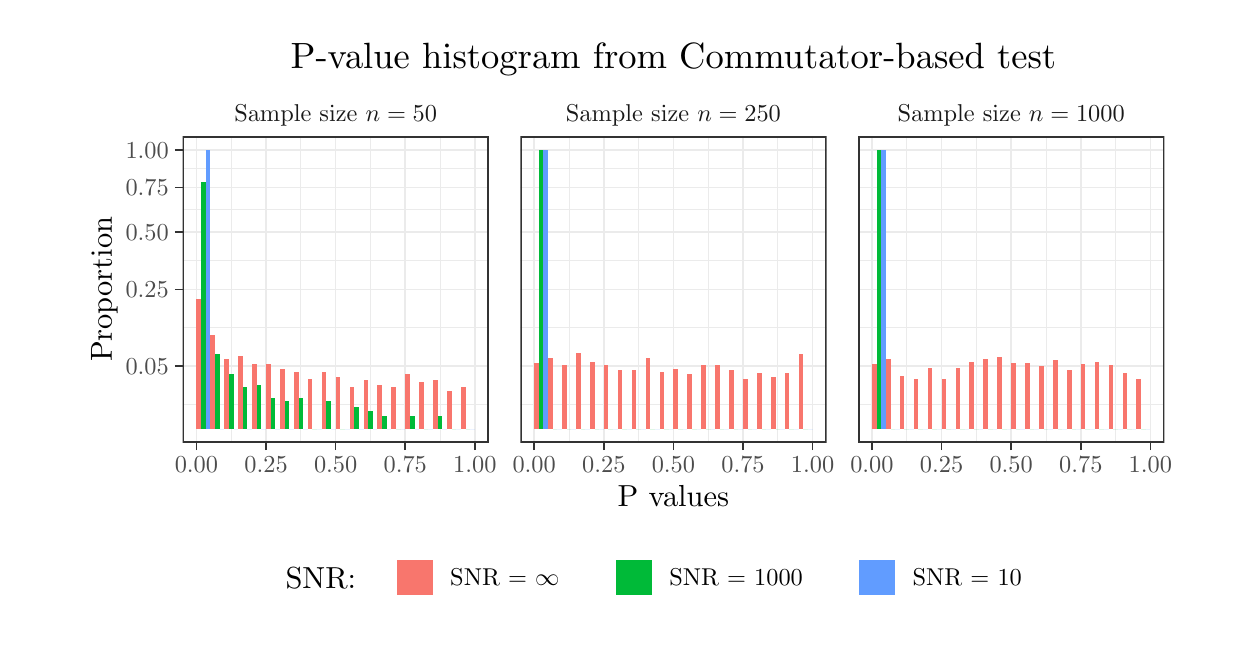
\begin{tikzpicture}[x=1pt,y=1pt]
\definecolor{fillColor}{RGB}{255,255,255}
\path[use as bounding box,fill=fillColor,fill opacity=0.00] (0,0) rectangle (433.62,216.81);
\begin{scope}
\path[clip] ( 17.40,  0.00) rectangle (416.22,216.81);
\definecolor{drawColor}{RGB}{255,255,255}
\definecolor{fillColor}{RGB}{255,255,255}

\path[draw=drawColor,line width= 0.6pt,line join=round,line cap=round,fill=fillColor] ( 17.40,  0.00) rectangle (416.22,216.81);
\end{scope}
\begin{scope}
\path[clip] ( 55.95, 66.91) rectangle (166.62,177.58);
\definecolor{fillColor}{RGB}{255,255,255}

\path[fill=fillColor] ( 55.95, 66.91) rectangle (166.62,177.58);
\definecolor{drawColor}{gray}{0.92}

\path[draw=drawColor,line width= 0.3pt,line join=round] ( 55.95, 80.54) --
	(166.62, 80.54);

\path[draw=drawColor,line width= 0.3pt,line join=round] ( 55.95,108.34) --
	(166.62,108.34);

\path[draw=drawColor,line width= 0.3pt,line join=round] ( 55.95,132.67) --
	(166.62,132.67);

\path[draw=drawColor,line width= 0.3pt,line join=round] ( 55.95,151.08) --
	(166.62,151.08);

\path[draw=drawColor,line width= 0.3pt,line join=round] ( 55.95,165.81) --
	(166.62,165.81);

\path[draw=drawColor,line width= 0.3pt,line join=round] ( 73.56, 66.91) --
	( 73.56,177.58);

\path[draw=drawColor,line width= 0.3pt,line join=round] ( 98.71, 66.91) --
	( 98.71,177.58);

\path[draw=drawColor,line width= 0.3pt,line join=round] (123.86, 66.91) --
	(123.86,177.58);

\path[draw=drawColor,line width= 0.3pt,line join=round] (149.02, 66.91) --
	(149.02,177.58);

\path[draw=drawColor,line width= 0.6pt,line join=round] ( 55.95, 94.44) --
	(166.62, 94.44);

\path[draw=drawColor,line width= 0.6pt,line join=round] ( 55.95,122.25) --
	(166.62,122.25);

\path[draw=drawColor,line width= 0.6pt,line join=round] ( 55.95,143.08) --
	(166.62,143.08);

\path[draw=drawColor,line width= 0.6pt,line join=round] ( 55.95,159.07) --
	(166.62,159.07);

\path[draw=drawColor,line width= 0.6pt,line join=round] ( 55.95,172.55) --
	(166.62,172.55);

\path[draw=drawColor,line width= 0.6pt,line join=round] ( 60.98, 66.91) --
	( 60.98,177.58);

\path[draw=drawColor,line width= 0.6pt,line join=round] ( 86.14, 66.91) --
	( 86.14,177.58);

\path[draw=drawColor,line width= 0.6pt,line join=round] (111.29, 66.91) --
	(111.29,177.58);

\path[draw=drawColor,line width= 0.6pt,line join=round] (136.44, 66.91) --
	(136.44,177.58);

\path[draw=drawColor,line width= 0.6pt,line join=round] (161.59, 66.91) --
	(161.59,177.58);
\definecolor{fillColor}{RGB}{248,118,109}

\path[fill=fillColor] ( 60.98, 71.94) rectangle ( 62.66,118.92);

\path[fill=fillColor] ( 66.01, 71.94) rectangle ( 67.69,105.91);

\path[fill=fillColor] ( 71.04, 71.94) rectangle ( 72.72, 96.99);

\path[fill=fillColor] ( 76.07, 71.94) rectangle ( 77.75, 98.18);

\path[fill=fillColor] ( 81.10, 71.94) rectangle ( 82.78, 95.32);

\path[fill=fillColor] ( 86.14, 71.94) rectangle ( 87.81, 95.32);

\path[fill=fillColor] ( 91.17, 71.94) rectangle ( 92.84, 93.52);

\path[fill=fillColor] ( 96.20, 71.94) rectangle ( 97.87, 92.56);

\path[fill=fillColor] (101.23, 71.94) rectangle (102.90, 89.94);

\path[fill=fillColor] (106.26, 71.94) rectangle (107.93, 92.56);

\path[fill=fillColor] (111.29, 71.94) rectangle (112.96, 90.49);

\path[fill=fillColor] (116.32, 71.94) rectangle (117.99, 86.87);

\path[fill=fillColor] (121.35, 71.94) rectangle (123.02, 89.37);

\path[fill=fillColor] (126.38, 71.94) rectangle (128.06, 87.53);

\path[fill=fillColor] (131.41, 71.94) rectangle (133.09, 86.87);

\path[fill=fillColor] (136.44, 71.94) rectangle (138.12, 91.55);

\path[fill=fillColor] (141.47, 71.94) rectangle (143.15, 88.78);

\path[fill=fillColor] (146.50, 71.94) rectangle (148.18, 89.37);

\path[fill=fillColor] (151.53, 71.94) rectangle (153.21, 85.44);

\path[fill=fillColor] (156.56, 71.94) rectangle (158.24, 86.87);
\definecolor{fillColor}{RGB}{0,186,56}

\path[fill=fillColor] ( 62.66, 71.94) rectangle ( 64.34,161.02);

\path[fill=fillColor] ( 67.69, 71.94) rectangle ( 69.37, 98.94);

\path[fill=fillColor] ( 72.72, 71.94) rectangle ( 74.40, 91.55);

\path[fill=fillColor] ( 77.75, 71.94) rectangle ( 79.43, 86.87);

\path[fill=fillColor] ( 82.78, 71.94) rectangle ( 84.46, 87.53);

\path[fill=fillColor] ( 87.81, 71.94) rectangle ( 89.49, 82.96);

\path[fill=fillColor] ( 92.84, 71.94) rectangle ( 94.52, 82.00);

\path[fill=fillColor] ( 97.87, 71.94) rectangle ( 99.55, 82.96);

\path[fill=fillColor] (102.90, 71.94) rectangle (104.58, 71.94);

\path[fill=fillColor] (107.93, 71.94) rectangle (109.61, 82.00);

\path[fill=fillColor] (112.96, 71.94) rectangle (114.64, 71.94);

\path[fill=fillColor] (117.99, 71.94) rectangle (119.67, 79.74);

\path[fill=fillColor] (123.02, 71.94) rectangle (124.70, 78.31);

\path[fill=fillColor] (128.06, 71.94) rectangle (129.73, 76.44);

\path[fill=fillColor] (133.09, 71.94) rectangle (134.76, 71.94);

\path[fill=fillColor] (138.12, 71.94) rectangle (139.79, 76.44);

\path[fill=fillColor] (143.15, 71.94) rectangle (144.82, 71.94);

\path[fill=fillColor] (148.18, 71.94) rectangle (149.85, 76.44);

\path[fill=fillColor] (153.21, 71.94) rectangle (154.88, 71.94);

\path[fill=fillColor] (158.24, 71.94) rectangle (159.91, 71.94);
\definecolor{fillColor}{RGB}{97,156,255}

\path[fill=fillColor] ( 64.34, 71.94) rectangle ( 66.01,172.55);

\path[fill=fillColor] ( 69.37, 71.94) rectangle ( 71.04, 71.94);

\path[fill=fillColor] ( 74.40, 71.94) rectangle ( 76.07, 71.94);

\path[fill=fillColor] ( 79.43, 71.94) rectangle ( 81.10, 71.94);

\path[fill=fillColor] ( 84.46, 71.94) rectangle ( 86.14, 71.94);

\path[fill=fillColor] ( 89.49, 71.94) rectangle ( 91.17, 71.94);

\path[fill=fillColor] ( 94.52, 71.94) rectangle ( 96.20, 71.94);

\path[fill=fillColor] ( 99.55, 71.94) rectangle (101.23, 71.94);

\path[fill=fillColor] (104.58, 71.94) rectangle (106.26, 71.94);

\path[fill=fillColor] (109.61, 71.94) rectangle (111.29, 71.94);

\path[fill=fillColor] (114.64, 71.94) rectangle (116.32, 71.94);

\path[fill=fillColor] (119.67, 71.94) rectangle (121.35, 71.94);

\path[fill=fillColor] (124.70, 71.94) rectangle (126.38, 71.94);

\path[fill=fillColor] (129.73, 71.94) rectangle (131.41, 71.94);

\path[fill=fillColor] (134.76, 71.94) rectangle (136.44, 71.94);

\path[fill=fillColor] (139.79, 71.94) rectangle (141.47, 71.94);

\path[fill=fillColor] (144.82, 71.94) rectangle (146.50, 71.94);

\path[fill=fillColor] (149.85, 71.94) rectangle (151.53, 71.94);

\path[fill=fillColor] (154.88, 71.94) rectangle (156.56, 71.94);

\path[fill=fillColor] (159.91, 71.94) rectangle (161.59, 71.94);
\definecolor{drawColor}{gray}{0.20}

\path[draw=drawColor,line width= 1.1pt,line join=round,line cap=round] ( 55.95, 66.91) rectangle (166.62,177.58);
\end{scope}
\begin{scope}
\path[clip] (178.00, 66.91) rectangle (288.67,177.58);
\definecolor{fillColor}{RGB}{255,255,255}

\path[fill=fillColor] (178.00, 66.91) rectangle (288.67,177.58);
\definecolor{drawColor}{gray}{0.92}

\path[draw=drawColor,line width= 0.3pt,line join=round] (178.00, 80.54) --
	(288.67, 80.54);

\path[draw=drawColor,line width= 0.3pt,line join=round] (178.00,108.34) --
	(288.67,108.34);

\path[draw=drawColor,line width= 0.3pt,line join=round] (178.00,132.67) --
	(288.67,132.67);

\path[draw=drawColor,line width= 0.3pt,line join=round] (178.00,151.08) --
	(288.67,151.08);

\path[draw=drawColor,line width= 0.3pt,line join=round] (178.00,165.81) --
	(288.67,165.81);

\path[draw=drawColor,line width= 0.3pt,line join=round] (195.61, 66.91) --
	(195.61,177.58);

\path[draw=drawColor,line width= 0.3pt,line join=round] (220.76, 66.91) --
	(220.76,177.58);

\path[draw=drawColor,line width= 0.3pt,line join=round] (245.91, 66.91) --
	(245.91,177.58);

\path[draw=drawColor,line width= 0.3pt,line join=round] (271.07, 66.91) --
	(271.07,177.58);

\path[draw=drawColor,line width= 0.6pt,line join=round] (178.00, 94.44) --
	(288.67, 94.44);

\path[draw=drawColor,line width= 0.6pt,line join=round] (178.00,122.25) --
	(288.67,122.25);

\path[draw=drawColor,line width= 0.6pt,line join=round] (178.00,143.08) --
	(288.67,143.08);

\path[draw=drawColor,line width= 0.6pt,line join=round] (178.00,159.07) --
	(288.67,159.07);

\path[draw=drawColor,line width= 0.6pt,line join=round] (178.00,172.55) --
	(288.67,172.55);

\path[draw=drawColor,line width= 0.6pt,line join=round] (183.03, 66.91) --
	(183.03,177.58);

\path[draw=drawColor,line width= 0.6pt,line join=round] (208.19, 66.91) --
	(208.19,177.58);

\path[draw=drawColor,line width= 0.6pt,line join=round] (233.34, 66.91) --
	(233.34,177.58);

\path[draw=drawColor,line width= 0.6pt,line join=round] (258.49, 66.91) --
	(258.49,177.58);

\path[draw=drawColor,line width= 0.6pt,line join=round] (283.64, 66.91) --
	(283.64,177.58);
\definecolor{fillColor}{RGB}{248,118,109}

\path[fill=fillColor] (183.03, 71.94) rectangle (184.71, 95.75);

\path[fill=fillColor] (188.06, 71.94) rectangle (189.74, 97.39);

\path[fill=fillColor] (193.09, 71.94) rectangle (194.77, 94.88);

\path[fill=fillColor] (198.12, 71.94) rectangle (199.80, 99.31);

\path[fill=fillColor] (203.16, 71.94) rectangle (204.83, 96.17);

\path[fill=fillColor] (208.19, 71.94) rectangle (209.86, 94.88);

\path[fill=fillColor] (213.22, 71.94) rectangle (214.89, 93.05);

\path[fill=fillColor] (218.25, 71.94) rectangle (219.92, 93.05);

\path[fill=fillColor] (223.28, 71.94) rectangle (224.95, 97.39);

\path[fill=fillColor] (228.31, 71.94) rectangle (229.98, 92.56);

\path[fill=fillColor] (233.34, 71.94) rectangle (235.01, 93.52);

\path[fill=fillColor] (238.37, 71.94) rectangle (240.04, 91.55);

\path[fill=fillColor] (243.40, 71.94) rectangle (245.08, 94.88);

\path[fill=fillColor] (248.43, 71.94) rectangle (250.11, 94.88);

\path[fill=fillColor] (253.46, 71.94) rectangle (255.14, 93.05);

\path[fill=fillColor] (258.49, 71.94) rectangle (260.17, 89.94);

\path[fill=fillColor] (263.52, 71.94) rectangle (265.20, 92.06);

\path[fill=fillColor] (268.55, 71.94) rectangle (270.23, 90.49);

\path[fill=fillColor] (273.58, 71.94) rectangle (275.26, 92.06);

\path[fill=fillColor] (278.61, 71.94) rectangle (280.29, 98.94);
\definecolor{fillColor}{RGB}{0,186,56}

\path[fill=fillColor] (184.71, 71.94) rectangle (186.39,172.55);

\path[fill=fillColor] (189.74, 71.94) rectangle (191.42, 71.94);

\path[fill=fillColor] (194.77, 71.94) rectangle (196.45, 71.94);

\path[fill=fillColor] (199.80, 71.94) rectangle (201.48, 71.94);

\path[fill=fillColor] (204.83, 71.94) rectangle (206.51, 71.94);

\path[fill=fillColor] (209.86, 71.94) rectangle (211.54, 71.94);

\path[fill=fillColor] (214.89, 71.94) rectangle (216.57, 71.94);

\path[fill=fillColor] (219.92, 71.94) rectangle (221.60, 71.94);

\path[fill=fillColor] (224.95, 71.94) rectangle (226.63, 71.94);

\path[fill=fillColor] (229.98, 71.94) rectangle (231.66, 71.94);

\path[fill=fillColor] (235.01, 71.94) rectangle (236.69, 71.94);

\path[fill=fillColor] (240.04, 71.94) rectangle (241.72, 71.94);

\path[fill=fillColor] (245.08, 71.94) rectangle (246.75, 71.94);

\path[fill=fillColor] (250.11, 71.94) rectangle (251.78, 71.94);

\path[fill=fillColor] (255.14, 71.94) rectangle (256.81, 71.94);

\path[fill=fillColor] (260.17, 71.94) rectangle (261.84, 71.94);

\path[fill=fillColor] (265.20, 71.94) rectangle (266.87, 71.94);

\path[fill=fillColor] (270.23, 71.94) rectangle (271.90, 71.94);

\path[fill=fillColor] (275.26, 71.94) rectangle (276.93, 71.94);

\path[fill=fillColor] (280.29, 71.94) rectangle (281.96, 71.94);
\definecolor{fillColor}{RGB}{97,156,255}

\path[fill=fillColor] (186.39, 71.94) rectangle (188.06,172.55);

\path[fill=fillColor] (191.42, 71.94) rectangle (193.09, 71.94);

\path[fill=fillColor] (196.45, 71.94) rectangle (198.12, 71.94);

\path[fill=fillColor] (201.48, 71.94) rectangle (203.16, 71.94);

\path[fill=fillColor] (206.51, 71.94) rectangle (208.19, 71.94);

\path[fill=fillColor] (211.54, 71.94) rectangle (213.22, 71.94);

\path[fill=fillColor] (216.57, 71.94) rectangle (218.25, 71.94);

\path[fill=fillColor] (221.60, 71.94) rectangle (223.28, 71.94);

\path[fill=fillColor] (226.63, 71.94) rectangle (228.31, 71.94);

\path[fill=fillColor] (231.66, 71.94) rectangle (233.34, 71.94);

\path[fill=fillColor] (236.69, 71.94) rectangle (238.37, 71.94);

\path[fill=fillColor] (241.72, 71.94) rectangle (243.40, 71.94);

\path[fill=fillColor] (246.75, 71.94) rectangle (248.43, 71.94);

\path[fill=fillColor] (251.78, 71.94) rectangle (253.46, 71.94);

\path[fill=fillColor] (256.81, 71.94) rectangle (258.49, 71.94);

\path[fill=fillColor] (261.84, 71.94) rectangle (263.52, 71.94);

\path[fill=fillColor] (266.87, 71.94) rectangle (268.55, 71.94);

\path[fill=fillColor] (271.90, 71.94) rectangle (273.58, 71.94);

\path[fill=fillColor] (276.93, 71.94) rectangle (278.61, 71.94);

\path[fill=fillColor] (281.96, 71.94) rectangle (283.64, 71.94);
\definecolor{drawColor}{gray}{0.20}

\path[draw=drawColor,line width= 1.1pt,line join=round,line cap=round] (178.00, 66.91) rectangle (288.67,177.58);
\end{scope}
\begin{scope}
\path[clip] (300.05, 66.91) rectangle (410.72,177.58);
\definecolor{fillColor}{RGB}{255,255,255}

\path[fill=fillColor] (300.05, 66.91) rectangle (410.72,177.58);
\definecolor{drawColor}{gray}{0.92}

\path[draw=drawColor,line width= 0.3pt,line join=round] (300.05, 80.54) --
	(410.72, 80.54);

\path[draw=drawColor,line width= 0.3pt,line join=round] (300.05,108.34) --
	(410.72,108.34);

\path[draw=drawColor,line width= 0.3pt,line join=round] (300.05,132.67) --
	(410.72,132.67);

\path[draw=drawColor,line width= 0.3pt,line join=round] (300.05,151.08) --
	(410.72,151.08);

\path[draw=drawColor,line width= 0.3pt,line join=round] (300.05,165.81) --
	(410.72,165.81);

\path[draw=drawColor,line width= 0.3pt,line join=round] (317.66, 66.91) --
	(317.66,177.58);

\path[draw=drawColor,line width= 0.3pt,line join=round] (342.81, 66.91) --
	(342.81,177.58);

\path[draw=drawColor,line width= 0.3pt,line join=round] (367.96, 66.91) --
	(367.96,177.58);

\path[draw=drawColor,line width= 0.3pt,line join=round] (393.12, 66.91) --
	(393.12,177.58);

\path[draw=drawColor,line width= 0.6pt,line join=round] (300.05, 94.44) --
	(410.72, 94.44);

\path[draw=drawColor,line width= 0.6pt,line join=round] (300.05,122.25) --
	(410.72,122.25);

\path[draw=drawColor,line width= 0.6pt,line join=round] (300.05,143.08) --
	(410.72,143.08);

\path[draw=drawColor,line width= 0.6pt,line join=round] (300.05,159.07) --
	(410.72,159.07);

\path[draw=drawColor,line width= 0.6pt,line join=round] (300.05,172.55) --
	(410.72,172.55);

\path[draw=drawColor,line width= 0.6pt,line join=round] (305.08, 66.91) --
	(305.08,177.58);

\path[draw=drawColor,line width= 0.6pt,line join=round] (330.24, 66.91) --
	(330.24,177.58);

\path[draw=drawColor,line width= 0.6pt,line join=round] (355.39, 66.91) --
	(355.39,177.58);

\path[draw=drawColor,line width= 0.6pt,line join=round] (380.54, 66.91) --
	(380.54,177.58);

\path[draw=drawColor,line width= 0.6pt,line join=round] (405.69, 66.91) --
	(405.69,177.58);
\definecolor{fillColor}{RGB}{248,118,109}

\path[fill=fillColor] (305.08, 71.94) rectangle (306.76, 95.32);

\path[fill=fillColor] (310.11, 71.94) rectangle (311.79, 96.99);

\path[fill=fillColor] (315.14, 71.94) rectangle (316.82, 91.03);

\path[fill=fillColor] (320.17, 71.94) rectangle (321.85, 89.94);

\path[fill=fillColor] (325.21, 71.94) rectangle (326.88, 93.98);

\path[fill=fillColor] (330.24, 71.94) rectangle (331.91, 89.94);

\path[fill=fillColor] (335.27, 71.94) rectangle (336.94, 93.98);

\path[fill=fillColor] (340.30, 71.94) rectangle (341.97, 96.17);

\path[fill=fillColor] (345.33, 71.94) rectangle (347.00, 96.99);

\path[fill=fillColor] (350.36, 71.94) rectangle (352.03, 97.79);

\path[fill=fillColor] (355.39, 71.94) rectangle (357.06, 95.75);

\path[fill=fillColor] (360.42, 71.94) rectangle (362.09, 95.75);

\path[fill=fillColor] (365.45, 71.94) rectangle (367.13, 94.44);

\path[fill=fillColor] (370.48, 71.94) rectangle (372.16, 96.59);

\path[fill=fillColor] (375.51, 71.94) rectangle (377.19, 93.05);

\path[fill=fillColor] (380.54, 71.94) rectangle (382.22, 95.32);

\path[fill=fillColor] (385.57, 71.94) rectangle (387.25, 96.17);

\path[fill=fillColor] (390.60, 71.94) rectangle (392.28, 94.88);

\path[fill=fillColor] (395.63, 71.94) rectangle (397.31, 92.06);

\path[fill=fillColor] (400.66, 71.94) rectangle (402.34, 89.94);
\definecolor{fillColor}{RGB}{0,186,56}

\path[fill=fillColor] (306.76, 71.94) rectangle (308.44,172.55);

\path[fill=fillColor] (311.79, 71.94) rectangle (313.47, 71.94);

\path[fill=fillColor] (316.82, 71.94) rectangle (318.50, 71.94);

\path[fill=fillColor] (321.85, 71.94) rectangle (323.53, 71.94);

\path[fill=fillColor] (326.88, 71.94) rectangle (328.56, 71.94);

\path[fill=fillColor] (331.91, 71.94) rectangle (333.59, 71.94);

\path[fill=fillColor] (336.94, 71.94) rectangle (338.62, 71.94);

\path[fill=fillColor] (341.97, 71.94) rectangle (343.65, 71.94);

\path[fill=fillColor] (347.00, 71.94) rectangle (348.68, 71.94);

\path[fill=fillColor] (352.03, 71.94) rectangle (353.71, 71.94);

\path[fill=fillColor] (357.06, 71.94) rectangle (358.74, 71.94);

\path[fill=fillColor] (362.09, 71.94) rectangle (363.77, 71.94);

\path[fill=fillColor] (367.13, 71.94) rectangle (368.80, 71.94);

\path[fill=fillColor] (372.16, 71.94) rectangle (373.83, 71.94);

\path[fill=fillColor] (377.19, 71.94) rectangle (378.86, 71.94);

\path[fill=fillColor] (382.22, 71.94) rectangle (383.89, 71.94);

\path[fill=fillColor] (387.25, 71.94) rectangle (388.92, 71.94);

\path[fill=fillColor] (392.28, 71.94) rectangle (393.95, 71.94);

\path[fill=fillColor] (397.31, 71.94) rectangle (398.98, 71.94);

\path[fill=fillColor] (402.34, 71.94) rectangle (404.02, 71.94);
\definecolor{fillColor}{RGB}{97,156,255}

\path[fill=fillColor] (308.44, 71.94) rectangle (310.11,172.55);

\path[fill=fillColor] (313.47, 71.94) rectangle (315.14, 71.94);

\path[fill=fillColor] (318.50, 71.94) rectangle (320.17, 71.94);

\path[fill=fillColor] (323.53, 71.94) rectangle (325.21, 71.94);

\path[fill=fillColor] (328.56, 71.94) rectangle (330.24, 71.94);

\path[fill=fillColor] (333.59, 71.94) rectangle (335.27, 71.94);

\path[fill=fillColor] (338.62, 71.94) rectangle (340.30, 71.94);

\path[fill=fillColor] (343.65, 71.94) rectangle (345.33, 71.94);

\path[fill=fillColor] (348.68, 71.94) rectangle (350.36, 71.94);

\path[fill=fillColor] (353.71, 71.94) rectangle (355.39, 71.94);

\path[fill=fillColor] (358.74, 71.94) rectangle (360.42, 71.94);

\path[fill=fillColor] (363.77, 71.94) rectangle (365.45, 71.94);

\path[fill=fillColor] (368.80, 71.94) rectangle (370.48, 71.94);

\path[fill=fillColor] (373.83, 71.94) rectangle (375.51, 71.94);

\path[fill=fillColor] (378.86, 71.94) rectangle (380.54, 71.94);

\path[fill=fillColor] (383.89, 71.94) rectangle (385.57, 71.94);

\path[fill=fillColor] (388.92, 71.94) rectangle (390.60, 71.94);

\path[fill=fillColor] (393.95, 71.94) rectangle (395.63, 71.94);

\path[fill=fillColor] (398.98, 71.94) rectangle (400.66, 71.94);

\path[fill=fillColor] (404.02, 71.94) rectangle (405.69, 71.94);
\definecolor{drawColor}{gray}{0.20}

\path[draw=drawColor,line width= 1.1pt,line join=round,line cap=round] (300.05, 66.91) rectangle (410.72,177.58);
\end{scope}
\begin{scope}
\path[clip] ( 55.95,177.58) rectangle (166.62,194.15);
\definecolor{fillColor}{RGB}{255,255,255}

\path[fill=fillColor] ( 55.95,177.58) rectangle (166.62,194.15);
\definecolor{drawColor}{gray}{0.10}

\node[text=drawColor,anchor=base,inner sep=0pt, outer sep=0pt, scale=  0.88] at (111.29,182.84) {Sample size $n = 50$};
\end{scope}
\begin{scope}
\path[clip] (178.00,177.58) rectangle (288.67,194.15);
\definecolor{fillColor}{RGB}{255,255,255}

\path[fill=fillColor] (178.00,177.58) rectangle (288.67,194.15);
\definecolor{drawColor}{gray}{0.10}

\node[text=drawColor,anchor=base,inner sep=0pt, outer sep=0pt, scale=  0.88] at (233.34,182.84) {Sample size $n = 250$};
\end{scope}
\begin{scope}
\path[clip] (300.05,177.58) rectangle (410.72,194.15);
\definecolor{fillColor}{RGB}{255,255,255}

\path[fill=fillColor] (300.05,177.58) rectangle (410.72,194.15);
\definecolor{drawColor}{gray}{0.10}

\node[text=drawColor,anchor=base,inner sep=0pt, outer sep=0pt, scale=  0.88] at (355.39,182.84) {Sample size $n = 1000$};
\end{scope}
\begin{scope}
\path[clip] (  0.00,  0.00) rectangle (433.62,216.81);
\definecolor{drawColor}{gray}{0.20}

\path[draw=drawColor,line width= 0.6pt,line join=round] ( 60.98, 64.16) --
	( 60.98, 66.91);

\path[draw=drawColor,line width= 0.6pt,line join=round] ( 86.14, 64.16) --
	( 86.14, 66.91);

\path[draw=drawColor,line width= 0.6pt,line join=round] (111.29, 64.16) --
	(111.29, 66.91);

\path[draw=drawColor,line width= 0.6pt,line join=round] (136.44, 64.16) --
	(136.44, 66.91);

\path[draw=drawColor,line width= 0.6pt,line join=round] (161.59, 64.16) --
	(161.59, 66.91);
\end{scope}
\begin{scope}
\path[clip] (  0.00,  0.00) rectangle (433.62,216.81);
\definecolor{drawColor}{gray}{0.30}

\node[text=drawColor,anchor=base,inner sep=0pt, outer sep=0pt, scale=  0.88] at ( 60.98, 55.90) {0.00};

\node[text=drawColor,anchor=base,inner sep=0pt, outer sep=0pt, scale=  0.88] at ( 86.14, 55.90) {0.25};

\node[text=drawColor,anchor=base,inner sep=0pt, outer sep=0pt, scale=  0.88] at (111.29, 55.90) {0.50};

\node[text=drawColor,anchor=base,inner sep=0pt, outer sep=0pt, scale=  0.88] at (136.44, 55.90) {0.75};

\node[text=drawColor,anchor=base,inner sep=0pt, outer sep=0pt, scale=  0.88] at (161.59, 55.90) {1.00};
\end{scope}
\begin{scope}
\path[clip] (  0.00,  0.00) rectangle (433.62,216.81);
\definecolor{drawColor}{gray}{0.20}

\path[draw=drawColor,line width= 0.6pt,line join=round] (183.03, 64.16) --
	(183.03, 66.91);

\path[draw=drawColor,line width= 0.6pt,line join=round] (208.19, 64.16) --
	(208.19, 66.91);

\path[draw=drawColor,line width= 0.6pt,line join=round] (233.34, 64.16) --
	(233.34, 66.91);

\path[draw=drawColor,line width= 0.6pt,line join=round] (258.49, 64.16) --
	(258.49, 66.91);

\path[draw=drawColor,line width= 0.6pt,line join=round] (283.64, 64.16) --
	(283.64, 66.91);
\end{scope}
\begin{scope}
\path[clip] (  0.00,  0.00) rectangle (433.62,216.81);
\definecolor{drawColor}{gray}{0.30}

\node[text=drawColor,anchor=base,inner sep=0pt, outer sep=0pt, scale=  0.88] at (183.03, 55.90) {0.00};

\node[text=drawColor,anchor=base,inner sep=0pt, outer sep=0pt, scale=  0.88] at (208.19, 55.90) {0.25};

\node[text=drawColor,anchor=base,inner sep=0pt, outer sep=0pt, scale=  0.88] at (233.34, 55.90) {0.50};

\node[text=drawColor,anchor=base,inner sep=0pt, outer sep=0pt, scale=  0.88] at (258.49, 55.90) {0.75};

\node[text=drawColor,anchor=base,inner sep=0pt, outer sep=0pt, scale=  0.88] at (283.64, 55.90) {1.00};
\end{scope}
\begin{scope}
\path[clip] (  0.00,  0.00) rectangle (433.62,216.81);
\definecolor{drawColor}{gray}{0.20}

\path[draw=drawColor,line width= 0.6pt,line join=round] (305.08, 64.16) --
	(305.08, 66.91);

\path[draw=drawColor,line width= 0.6pt,line join=round] (330.24, 64.16) --
	(330.24, 66.91);

\path[draw=drawColor,line width= 0.6pt,line join=round] (355.39, 64.16) --
	(355.39, 66.91);

\path[draw=drawColor,line width= 0.6pt,line join=round] (380.54, 64.16) --
	(380.54, 66.91);

\path[draw=drawColor,line width= 0.6pt,line join=round] (405.69, 64.16) --
	(405.69, 66.91);
\end{scope}
\begin{scope}
\path[clip] (  0.00,  0.00) rectangle (433.62,216.81);
\definecolor{drawColor}{gray}{0.30}

\node[text=drawColor,anchor=base,inner sep=0pt, outer sep=0pt, scale=  0.88] at (305.08, 55.90) {0.00};

\node[text=drawColor,anchor=base,inner sep=0pt, outer sep=0pt, scale=  0.88] at (330.24, 55.90) {0.25};

\node[text=drawColor,anchor=base,inner sep=0pt, outer sep=0pt, scale=  0.88] at (355.39, 55.90) {0.50};

\node[text=drawColor,anchor=base,inner sep=0pt, outer sep=0pt, scale=  0.88] at (380.54, 55.90) {0.75};

\node[text=drawColor,anchor=base,inner sep=0pt, outer sep=0pt, scale=  0.88] at (405.69, 55.90) {1.00};
\end{scope}
\begin{scope}
\path[clip] (  0.00,  0.00) rectangle (433.62,216.81);
\definecolor{drawColor}{gray}{0.30}

\node[text=drawColor,anchor=base east,inner sep=0pt, outer sep=0pt, scale=  0.88] at ( 51.00, 91.41) {0.05};

\node[text=drawColor,anchor=base east,inner sep=0pt, outer sep=0pt, scale=  0.88] at ( 51.00,119.22) {0.25};

\node[text=drawColor,anchor=base east,inner sep=0pt, outer sep=0pt, scale=  0.88] at ( 51.00,140.05) {0.50};

\node[text=drawColor,anchor=base east,inner sep=0pt, outer sep=0pt, scale=  0.88] at ( 51.00,156.04) {0.75};

\node[text=drawColor,anchor=base east,inner sep=0pt, outer sep=0pt, scale=  0.88] at ( 51.00,169.52) {1.00};
\end{scope}
\begin{scope}
\path[clip] (  0.00,  0.00) rectangle (433.62,216.81);
\definecolor{drawColor}{gray}{0.20}

\path[draw=drawColor,line width= 0.6pt,line join=round] ( 53.20, 94.44) --
	( 55.95, 94.44);

\path[draw=drawColor,line width= 0.6pt,line join=round] ( 53.20,122.25) --
	( 55.95,122.25);

\path[draw=drawColor,line width= 0.6pt,line join=round] ( 53.20,143.08) --
	( 55.95,143.08);

\path[draw=drawColor,line width= 0.6pt,line join=round] ( 53.20,159.07) --
	( 55.95,159.07);

\path[draw=drawColor,line width= 0.6pt,line join=round] ( 53.20,172.55) --
	( 55.95,172.55);
\end{scope}
\begin{scope}
\path[clip] (  0.00,  0.00) rectangle (433.62,216.81);
\definecolor{drawColor}{RGB}{0,0,0}

\node[text=drawColor,anchor=base,inner sep=0pt, outer sep=0pt, scale=  1.10] at (233.34, 43.86) {P values};
\end{scope}
\begin{scope}
\path[clip] (  0.00,  0.00) rectangle (433.62,216.81);
\definecolor{drawColor}{RGB}{0,0,0}

\node[text=drawColor,rotate= 90.00,anchor=base,inner sep=0pt, outer sep=0pt, scale=  1.10] at ( 30.47,122.25) {Proportion};
\end{scope}
\begin{scope}
\path[clip] (  0.00,  0.00) rectangle (433.62,216.81);
\definecolor{fillColor}{RGB}{255,255,255}

\path[fill=fillColor] ( 87.69,  5.50) rectangle (378.98, 30.73);
\end{scope}
\begin{scope}
\path[clip] (  0.00,  0.00) rectangle (433.62,216.81);
\definecolor{drawColor}{RGB}{0,0,0}

\node[text=drawColor,anchor=base west,inner sep=0pt, outer sep=0pt, scale=  1.10] at ( 93.19, 14.33) {SNR:};
\end{scope}
\begin{scope}
\path[clip] (  0.00,  0.00) rectangle (433.62,216.81);
\definecolor{fillColor}{RGB}{255,255,255}

\path[fill=fillColor] (132.74, 11.00) rectangle (147.19, 25.23);
\end{scope}
\begin{scope}
\path[clip] (  0.00,  0.00) rectangle (433.62,216.81);
\definecolor{fillColor}{RGB}{248,118,109}

\path[fill=fillColor] (133.45, 11.71) rectangle (146.48, 24.52);
\end{scope}
\begin{scope}
\path[clip] (  0.00,  0.00) rectangle (433.62,216.81);
\definecolor{fillColor}{RGB}{255,255,255}

\path[fill=fillColor] (211.89, 11.00) rectangle (226.34, 25.23);
\end{scope}
\begin{scope}
\path[clip] (  0.00,  0.00) rectangle (433.62,216.81);
\definecolor{fillColor}{RGB}{0,186,56}

\path[fill=fillColor] (212.60, 11.71) rectangle (225.63, 24.52);
\end{scope}
\begin{scope}
\path[clip] (  0.00,  0.00) rectangle (433.62,216.81);
\definecolor{fillColor}{RGB}{255,255,255}

\path[fill=fillColor] (299.83, 11.00) rectangle (314.29, 25.23);
\end{scope}
\begin{scope}
\path[clip] (  0.00,  0.00) rectangle (433.62,216.81);
\definecolor{fillColor}{RGB}{97,156,255}

\path[fill=fillColor] (300.55, 11.71) rectangle (313.58, 24.52);
\end{scope}
\begin{scope}
\path[clip] (  0.00,  0.00) rectangle (433.62,216.81);
\definecolor{drawColor}{RGB}{0,0,0}

\node[text=drawColor,anchor=base west,inner sep=0pt, outer sep=0pt, scale=  0.88] at (152.69, 15.08) {SNR = $\infty$};
\end{scope}
\begin{scope}
\path[clip] (  0.00,  0.00) rectangle (433.62,216.81);
\definecolor{drawColor}{RGB}{0,0,0}

\node[text=drawColor,anchor=base west,inner sep=0pt, outer sep=0pt, scale=  0.88] at (231.84, 15.08) {SNR = 1000};
\end{scope}
\begin{scope}
\path[clip] (  0.00,  0.00) rectangle (433.62,216.81);
\definecolor{drawColor}{RGB}{0,0,0}

\node[text=drawColor,anchor=base west,inner sep=0pt, outer sep=0pt, scale=  0.88] at (319.79, 15.08) {SNR = 10};
\end{scope}
\begin{scope}
\path[clip] (  0.00,  0.00) rectangle (433.62,216.81);
\definecolor{drawColor}{RGB}{0,0,0}

\node[text=drawColor,anchor=base,inner sep=0pt, outer sep=0pt, scale=  1.32] at (233.34,202.22) {P-value histogram from Commutator-based test};
\end{scope}
\end{tikzpicture}
}
    \caption{The histograms of p-values for the commutator-based test in \autoref{thm:comm.Est} with simulated data.}
   \label{fig:comm}
\end{figure}

For the commutator-based test \autoref{thm:comm.Est}, we see from \autoref{fig:comm} that with sample size increasing, the p-values of samples from null space ($\SNR = \infty$) tend to be uniformly distributed on the interval $[0,1]$, and the p-values of samples from alternative spaces start to concentrate in the interval $[0, 0.05)$. When the sample size $n$ exceeds a certain level, $200$ for instance, the test performs well with acceptable type I error and excellent type II error.


\vspace{-0.5cm}
\subsection{Multi-sample test} \label{se:sim-multi}
\vspace{-0.3cm}
For the simulation study of the multi-sample test introduced in \autoref{sec:multi}, we follow \autoref{algo:DGP} to set the mean matrices of normally distributed observations as $\mathcal{M}_p(\rho, d; d)$. We consider here the setting that dimension $d = 4$, $p = 8$, $\SNR = \frac{1}{\rho^2} \in \{10, 100, 1000, \infty\}$, and sample size $n \in \{10^2, 10^3, 10^4, 10^5\}$. Each consistent estimate in $\mathcal{A}(\rho)$ is the empirical average from the $n$ observations, hence $c(n) = \sqrt{n}$ by the CLT. Note that when $\rho = 0$, equivalently $\SNR = \infty$, the matrices in $\mathcal{A}_p(\rho)$ satisfy $H_0$, i.e., share common eigenvectors.

To verify the testing efficiency, we (i) use the exact $V = V(d; d)$ (see \cref{step:commonV} of \autoref{algo:DGP}) to test on $\mathcal{A}_p(0)$ according to \autoref{thm:multi_eig.Est}, and (ii) use the optimized $\widehat{V}$ from algorithm '\textit{(W)JDTE}' and implement both \autoref{thm:multi_eig.Est} and \autoref{cor:multi}. We present the test power versus $\SNR$ and sample size $n$ through histogram plots; see \autoref{fig:multi}.

\begin{figure}[htbp] %  figure placement: here, top, bottom, or page
    \centering
    \centerline{% Created by tikzDevice version 0.12.3.1 on 2022-11-01 18:25:30
% !TEX encoding = UTF-8 Unicode
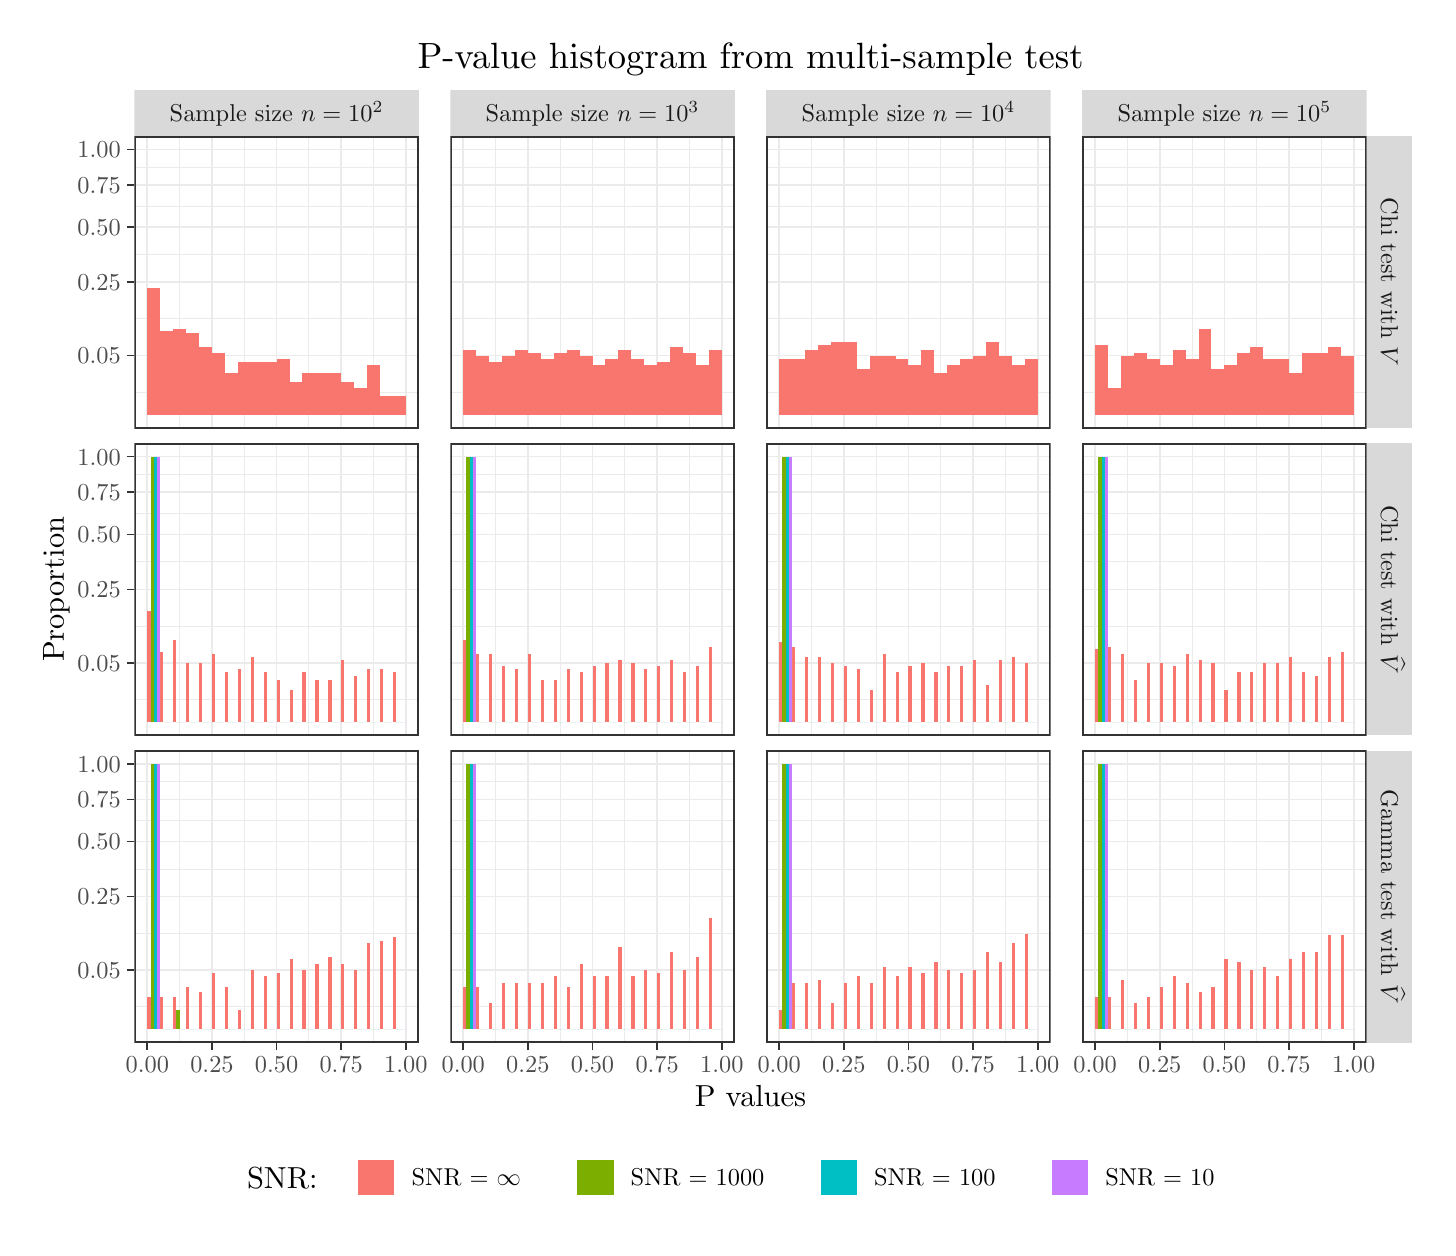
\begin{tikzpicture}[x=1pt,y=1pt]
\definecolor{fillColor}{RGB}{255,255,255}
\path[use as bounding box,fill=fillColor,fill opacity=0.00] (0,0) rectangle (505.89,433.62);
\begin{scope}
\path[clip] (  0.00,  0.00) rectangle (505.89,433.62);
\definecolor{drawColor}{RGB}{255,255,255}
\definecolor{fillColor}{RGB}{255,255,255}

\path[draw=drawColor,line width= 0.6pt,line join=round,line cap=round,fill=fillColor] ( -0.00,  0.00) rectangle (505.89,433.62);
\end{scope}
\begin{scope}
\path[clip] ( 38.56,288.90) rectangle (141.34,394.39);
\definecolor{fillColor}{RGB}{255,255,255}

\path[fill=fillColor] ( 38.56,288.90) rectangle (141.34,394.39);
\definecolor{drawColor}{gray}{0.92}

\path[draw=drawColor,line width= 0.3pt,line join=round] ( 38.56,301.88) --
	(141.34,301.88);

\path[draw=drawColor,line width= 0.3pt,line join=round] ( 38.56,328.39) --
	(141.34,328.39);

\path[draw=drawColor,line width= 0.3pt,line join=round] ( 38.56,351.58) --
	(141.34,351.58);

\path[draw=drawColor,line width= 0.3pt,line join=round] ( 38.56,369.13) --
	(141.34,369.13);

\path[draw=drawColor,line width= 0.3pt,line join=round] ( 38.56,383.17) --
	(141.34,383.17);

\path[draw=drawColor,line width= 0.3pt,line join=round] ( 54.91,288.90) --
	( 54.91,394.39);

\path[draw=drawColor,line width= 0.3pt,line join=round] ( 78.27,288.90) --
	( 78.27,394.39);

\path[draw=drawColor,line width= 0.3pt,line join=round] (101.62,288.90) --
	(101.62,394.39);

\path[draw=drawColor,line width= 0.3pt,line join=round] (124.98,288.90) --
	(124.98,394.39);

\path[draw=drawColor,line width= 0.6pt,line join=round] ( 38.56,315.14) --
	(141.34,315.14);

\path[draw=drawColor,line width= 0.6pt,line join=round] ( 38.56,341.64) --
	(141.34,341.64);

\path[draw=drawColor,line width= 0.6pt,line join=round] ( 38.56,361.51) --
	(141.34,361.51);

\path[draw=drawColor,line width= 0.6pt,line join=round] ( 38.56,376.75) --
	(141.34,376.75);

\path[draw=drawColor,line width= 0.6pt,line join=round] ( 38.56,389.60) --
	(141.34,389.60);

\path[draw=drawColor,line width= 0.6pt,line join=round] ( 43.23,288.90) --
	( 43.23,394.39);

\path[draw=drawColor,line width= 0.6pt,line join=round] ( 66.59,288.90) --
	( 66.59,394.39);

\path[draw=drawColor,line width= 0.6pt,line join=round] ( 89.95,288.90) --
	( 89.95,394.39);

\path[draw=drawColor,line width= 0.6pt,line join=round] (113.30,288.90) --
	(113.30,394.39);

\path[draw=drawColor,line width= 0.6pt,line join=round] (136.66,288.90) --
	(136.66,394.39);
\definecolor{fillColor}{RGB}{248,118,109}

\path[fill=fillColor] ( 43.23,293.69) rectangle ( 47.90,339.69);

\path[fill=fillColor] ( 47.90,293.69) rectangle ( 52.57,324.02);

\path[fill=fillColor] ( 52.57,293.69) rectangle ( 57.24,324.77);

\path[fill=fillColor] ( 57.24,293.69) rectangle ( 61.91,323.25);

\path[fill=fillColor] ( 61.91,293.69) rectangle ( 66.59,318.14);

\path[fill=fillColor] ( 66.59,293.69) rectangle ( 71.26,316.18);

\path[fill=fillColor] ( 71.26,293.69) rectangle ( 75.93,308.86);

\path[fill=fillColor] ( 75.93,293.69) rectangle ( 80.60,312.87);

\path[fill=fillColor] ( 80.60,293.69) rectangle ( 85.27,312.87);

\path[fill=fillColor] ( 85.27,293.69) rectangle ( 89.95,312.87);

\path[fill=fillColor] ( 89.95,293.69) rectangle ( 94.62,314.04);

\path[fill=fillColor] ( 94.62,293.69) rectangle ( 99.29,305.44);

\path[fill=fillColor] ( 99.29,293.69) rectangle (103.96,308.86);

\path[fill=fillColor] (103.96,293.69) rectangle (108.63,308.86);

\path[fill=fillColor] (108.63,293.69) rectangle (113.30,308.86);

\path[fill=fillColor] (113.30,293.69) rectangle (117.98,305.44);

\path[fill=fillColor] (117.98,293.69) rectangle (122.65,303.28);

\path[fill=fillColor] (122.65,293.69) rectangle (127.32,311.64);

\path[fill=fillColor] (127.32,293.69) rectangle (131.99,300.47);

\path[fill=fillColor] (131.99,293.69) rectangle (136.66,300.47);
\definecolor{drawColor}{gray}{0.20}

\path[draw=drawColor,line width= 1.1pt,line join=round,line cap=round] ( 38.56,288.90) rectangle (141.34,394.39);
\end{scope}
\begin{scope}
\path[clip] ( 38.56,177.91) rectangle (141.34,283.40);
\definecolor{fillColor}{RGB}{255,255,255}

\path[fill=fillColor] ( 38.56,177.91) rectangle (141.34,283.40);
\definecolor{drawColor}{gray}{0.92}

\path[draw=drawColor,line width= 0.3pt,line join=round] ( 38.56,190.89) --
	(141.34,190.89);

\path[draw=drawColor,line width= 0.3pt,line join=round] ( 38.56,217.40) --
	(141.34,217.40);

\path[draw=drawColor,line width= 0.3pt,line join=round] ( 38.56,240.58) --
	(141.34,240.58);

\path[draw=drawColor,line width= 0.3pt,line join=round] ( 38.56,258.13) --
	(141.34,258.13);

\path[draw=drawColor,line width= 0.3pt,line join=round] ( 38.56,272.18) --
	(141.34,272.18);

\path[draw=drawColor,line width= 0.3pt,line join=round] ( 54.91,177.91) --
	( 54.91,283.40);

\path[draw=drawColor,line width= 0.3pt,line join=round] ( 78.27,177.91) --
	( 78.27,283.40);

\path[draw=drawColor,line width= 0.3pt,line join=round] (101.62,177.91) --
	(101.62,283.40);

\path[draw=drawColor,line width= 0.3pt,line join=round] (124.98,177.91) --
	(124.98,283.40);

\path[draw=drawColor,line width= 0.6pt,line join=round] ( 38.56,204.14) --
	(141.34,204.14);

\path[draw=drawColor,line width= 0.6pt,line join=round] ( 38.56,230.65) --
	(141.34,230.65);

\path[draw=drawColor,line width= 0.6pt,line join=round] ( 38.56,250.51) --
	(141.34,250.51);

\path[draw=drawColor,line width= 0.6pt,line join=round] ( 38.56,265.75) --
	(141.34,265.75);

\path[draw=drawColor,line width= 0.6pt,line join=round] ( 38.56,278.60) --
	(141.34,278.60);

\path[draw=drawColor,line width= 0.6pt,line join=round] ( 43.23,177.91) --
	( 43.23,283.40);

\path[draw=drawColor,line width= 0.6pt,line join=round] ( 66.59,177.91) --
	( 66.59,283.40);

\path[draw=drawColor,line width= 0.6pt,line join=round] ( 89.95,177.91) --
	( 89.95,283.40);

\path[draw=drawColor,line width= 0.6pt,line join=round] (113.30,177.91) --
	(113.30,283.40);

\path[draw=drawColor,line width= 0.6pt,line join=round] (136.66,177.91) --
	(136.66,283.40);
\definecolor{fillColor}{RGB}{248,118,109}

\path[fill=fillColor] ( 43.23,182.70) rectangle ( 44.39,222.82);

\path[fill=fillColor] ( 47.90,182.70) rectangle ( 49.07,208.07);

\path[fill=fillColor] ( 52.57,182.70) rectangle ( 53.74,212.26);

\path[fill=fillColor] ( 57.24,182.70) rectangle ( 58.41,204.14);

\path[fill=fillColor] ( 61.91,182.70) rectangle ( 63.08,204.14);

\path[fill=fillColor] ( 66.59,182.70) rectangle ( 67.75,207.15);

\path[fill=fillColor] ( 71.26,182.70) rectangle ( 72.43,200.64);

\path[fill=fillColor] ( 75.93,182.70) rectangle ( 77.10,201.88);

\path[fill=fillColor] ( 80.60,182.70) rectangle ( 81.77,206.19);

\path[fill=fillColor] ( 85.27,182.70) rectangle ( 86.44,200.64);

\path[fill=fillColor] ( 89.95,182.70) rectangle ( 91.11,197.86);

\path[fill=fillColor] ( 94.62,182.70) rectangle ( 95.78,194.45);

\path[fill=fillColor] ( 99.29,182.70) rectangle (100.46,200.64);

\path[fill=fillColor] (103.96,182.70) rectangle (105.13,197.86);

\path[fill=fillColor] (108.63,182.70) rectangle (109.80,197.86);

\path[fill=fillColor] (113.30,182.70) rectangle (114.47,205.19);

\path[fill=fillColor] (117.98,182.70) rectangle (119.14,199.31);

\path[fill=fillColor] (122.65,182.70) rectangle (123.82,201.88);

\path[fill=fillColor] (127.32,182.70) rectangle (128.49,201.88);

\path[fill=fillColor] (131.99,182.70) rectangle (133.16,200.64);
\definecolor{fillColor}{RGB}{124,174,0}

\path[fill=fillColor] ( 44.39,182.70) rectangle ( 45.56,278.60);

\path[fill=fillColor] ( 49.07,182.70) rectangle ( 50.23,182.70);

\path[fill=fillColor] ( 53.74,182.70) rectangle ( 54.91,182.70);

\path[fill=fillColor] ( 58.41,182.70) rectangle ( 59.58,182.70);

\path[fill=fillColor] ( 63.08,182.70) rectangle ( 64.25,182.70);

\path[fill=fillColor] ( 67.75,182.70) rectangle ( 68.92,182.70);

\path[fill=fillColor] ( 72.43,182.70) rectangle ( 73.59,182.70);

\path[fill=fillColor] ( 77.10,182.70) rectangle ( 78.27,182.70);

\path[fill=fillColor] ( 81.77,182.70) rectangle ( 82.94,182.70);

\path[fill=fillColor] ( 86.44,182.70) rectangle ( 87.61,182.70);

\path[fill=fillColor] ( 91.11,182.70) rectangle ( 92.28,182.70);

\path[fill=fillColor] ( 95.78,182.70) rectangle ( 96.95,182.70);

\path[fill=fillColor] (100.46,182.70) rectangle (101.62,182.70);

\path[fill=fillColor] (105.13,182.70) rectangle (106.30,182.70);

\path[fill=fillColor] (109.80,182.70) rectangle (110.97,182.70);

\path[fill=fillColor] (114.47,182.70) rectangle (115.64,182.70);

\path[fill=fillColor] (119.14,182.70) rectangle (120.31,182.70);

\path[fill=fillColor] (123.82,182.70) rectangle (124.98,182.70);

\path[fill=fillColor] (128.49,182.70) rectangle (129.66,182.70);

\path[fill=fillColor] (133.16,182.70) rectangle (134.33,182.70);
\definecolor{fillColor}{RGB}{0,191,196}

\path[fill=fillColor] ( 45.56,182.70) rectangle ( 46.73,278.60);

\path[fill=fillColor] ( 50.23,182.70) rectangle ( 51.40,182.70);

\path[fill=fillColor] ( 54.91,182.70) rectangle ( 56.07,182.70);

\path[fill=fillColor] ( 59.58,182.70) rectangle ( 60.75,182.70);

\path[fill=fillColor] ( 64.25,182.70) rectangle ( 65.42,182.70);

\path[fill=fillColor] ( 68.92,182.70) rectangle ( 70.09,182.70);

\path[fill=fillColor] ( 73.59,182.70) rectangle ( 74.76,182.70);

\path[fill=fillColor] ( 78.27,182.70) rectangle ( 79.43,182.70);

\path[fill=fillColor] ( 82.94,182.70) rectangle ( 84.11,182.70);

\path[fill=fillColor] ( 87.61,182.70) rectangle ( 88.78,182.70);

\path[fill=fillColor] ( 92.28,182.70) rectangle ( 93.45,182.70);

\path[fill=fillColor] ( 96.95,182.70) rectangle ( 98.12,182.70);

\path[fill=fillColor] (101.62,182.70) rectangle (102.79,182.70);

\path[fill=fillColor] (106.30,182.70) rectangle (107.46,182.70);

\path[fill=fillColor] (110.97,182.70) rectangle (112.14,182.70);

\path[fill=fillColor] (115.64,182.70) rectangle (116.81,182.70);

\path[fill=fillColor] (120.31,182.70) rectangle (121.48,182.70);

\path[fill=fillColor] (124.98,182.70) rectangle (126.15,182.70);

\path[fill=fillColor] (129.66,182.70) rectangle (130.82,182.70);

\path[fill=fillColor] (134.33,182.70) rectangle (135.50,182.70);
\definecolor{fillColor}{RGB}{199,124,255}

\path[fill=fillColor] ( 46.73,182.70) rectangle ( 47.90,278.60);

\path[fill=fillColor] ( 51.40,182.70) rectangle ( 52.57,182.70);

\path[fill=fillColor] ( 56.07,182.70) rectangle ( 57.24,182.70);

\path[fill=fillColor] ( 60.75,182.70) rectangle ( 61.91,182.70);

\path[fill=fillColor] ( 65.42,182.70) rectangle ( 66.59,182.70);

\path[fill=fillColor] ( 70.09,182.70) rectangle ( 71.26,182.70);

\path[fill=fillColor] ( 74.76,182.70) rectangle ( 75.93,182.70);

\path[fill=fillColor] ( 79.43,182.70) rectangle ( 80.60,182.70);

\path[fill=fillColor] ( 84.11,182.70) rectangle ( 85.27,182.70);

\path[fill=fillColor] ( 88.78,182.70) rectangle ( 89.95,182.70);

\path[fill=fillColor] ( 93.45,182.70) rectangle ( 94.62,182.70);

\path[fill=fillColor] ( 98.12,182.70) rectangle ( 99.29,182.70);

\path[fill=fillColor] (102.79,182.70) rectangle (103.96,182.70);

\path[fill=fillColor] (107.46,182.70) rectangle (108.63,182.70);

\path[fill=fillColor] (112.14,182.70) rectangle (113.30,182.70);

\path[fill=fillColor] (116.81,182.70) rectangle (117.98,182.70);

\path[fill=fillColor] (121.48,182.70) rectangle (122.65,182.70);

\path[fill=fillColor] (126.15,182.70) rectangle (127.32,182.70);

\path[fill=fillColor] (130.82,182.70) rectangle (131.99,182.70);

\path[fill=fillColor] (135.50,182.70) rectangle (136.66,182.70);
\definecolor{drawColor}{gray}{0.20}

\path[draw=drawColor,line width= 1.1pt,line join=round,line cap=round] ( 38.56,177.91) rectangle (141.34,283.40);
\end{scope}
\begin{scope}
\path[clip] ( 38.56, 66.91) rectangle (141.34,172.41);
\definecolor{fillColor}{RGB}{255,255,255}

\path[fill=fillColor] ( 38.56, 66.91) rectangle (141.34,172.41);
\definecolor{drawColor}{gray}{0.92}

\path[draw=drawColor,line width= 0.3pt,line join=round] ( 38.56, 79.90) --
	(141.34, 79.90);

\path[draw=drawColor,line width= 0.3pt,line join=round] ( 38.56,106.41) --
	(141.34,106.41);

\path[draw=drawColor,line width= 0.3pt,line join=round] ( 38.56,129.59) --
	(141.34,129.59);

\path[draw=drawColor,line width= 0.3pt,line join=round] ( 38.56,147.14) --
	(141.34,147.14);

\path[draw=drawColor,line width= 0.3pt,line join=round] ( 38.56,161.19) --
	(141.34,161.19);

\path[draw=drawColor,line width= 0.3pt,line join=round] ( 54.91, 66.91) --
	( 54.91,172.41);

\path[draw=drawColor,line width= 0.3pt,line join=round] ( 78.27, 66.91) --
	( 78.27,172.41);

\path[draw=drawColor,line width= 0.3pt,line join=round] (101.62, 66.91) --
	(101.62,172.41);

\path[draw=drawColor,line width= 0.3pt,line join=round] (124.98, 66.91) --
	(124.98,172.41);

\path[draw=drawColor,line width= 0.6pt,line join=round] ( 38.56, 93.15) --
	(141.34, 93.15);

\path[draw=drawColor,line width= 0.6pt,line join=round] ( 38.56,119.66) --
	(141.34,119.66);

\path[draw=drawColor,line width= 0.6pt,line join=round] ( 38.56,139.52) --
	(141.34,139.52);

\path[draw=drawColor,line width= 0.6pt,line join=round] ( 38.56,154.76) --
	(141.34,154.76);

\path[draw=drawColor,line width= 0.6pt,line join=round] ( 38.56,167.61) --
	(141.34,167.61);

\path[draw=drawColor,line width= 0.6pt,line join=round] ( 43.23, 66.91) --
	( 43.23,172.41);

\path[draw=drawColor,line width= 0.6pt,line join=round] ( 66.59, 66.91) --
	( 66.59,172.41);

\path[draw=drawColor,line width= 0.6pt,line join=round] ( 89.95, 66.91) --
	( 89.95,172.41);

\path[draw=drawColor,line width= 0.6pt,line join=round] (113.30, 66.91) --
	(113.30,172.41);

\path[draw=drawColor,line width= 0.6pt,line join=round] (136.66, 66.91) --
	(136.66,172.41);
\definecolor{fillColor}{RGB}{248,118,109}

\path[fill=fillColor] ( 43.23, 71.71) rectangle ( 44.39, 83.45);

\path[fill=fillColor] ( 47.90, 71.71) rectangle ( 49.07, 83.45);

\path[fill=fillColor] ( 52.57, 71.71) rectangle ( 53.74, 83.45);

\path[fill=fillColor] ( 57.24, 71.71) rectangle ( 58.41, 86.87);

\path[fill=fillColor] ( 61.91, 71.71) rectangle ( 63.08, 85.27);

\path[fill=fillColor] ( 66.59, 71.71) rectangle ( 67.75, 92.05);

\path[fill=fillColor] ( 71.26, 71.71) rectangle ( 72.43, 86.87);

\path[fill=fillColor] ( 75.93, 71.71) rectangle ( 77.10, 78.49);

\path[fill=fillColor] ( 80.60, 71.71) rectangle ( 81.77, 93.15);

\path[fill=fillColor] ( 85.27, 71.71) rectangle ( 86.44, 90.89);

\path[fill=fillColor] ( 89.95, 71.71) rectangle ( 91.11, 92.05);

\path[fill=fillColor] ( 94.62, 71.71) rectangle ( 95.78, 97.08);

\path[fill=fillColor] ( 99.29, 71.71) rectangle (100.46, 93.15);

\path[fill=fillColor] (103.96, 71.71) rectangle (105.13, 95.20);

\path[fill=fillColor] (108.63, 71.71) rectangle (109.80, 97.97);

\path[fill=fillColor] (113.30, 71.71) rectangle (114.47, 95.20);

\path[fill=fillColor] (117.98, 71.71) rectangle (119.14, 93.15);

\path[fill=fillColor] (122.65, 71.71) rectangle (123.82,102.78);

\path[fill=fillColor] (127.32, 71.71) rectangle (128.49,103.51);

\path[fill=fillColor] (131.99, 71.71) rectangle (133.16,104.93);
\definecolor{fillColor}{RGB}{124,174,0}

\path[fill=fillColor] ( 44.39, 71.71) rectangle ( 45.56,167.37);

\path[fill=fillColor] ( 49.07, 71.71) rectangle ( 50.23, 71.71);

\path[fill=fillColor] ( 53.74, 71.71) rectangle ( 54.91, 78.49);

\path[fill=fillColor] ( 58.41, 71.71) rectangle ( 59.58, 71.71);

\path[fill=fillColor] ( 63.08, 71.71) rectangle ( 64.25, 71.71);

\path[fill=fillColor] ( 67.75, 71.71) rectangle ( 68.92, 71.71);

\path[fill=fillColor] ( 72.43, 71.71) rectangle ( 73.59, 71.71);

\path[fill=fillColor] ( 77.10, 71.71) rectangle ( 78.27, 71.71);

\path[fill=fillColor] ( 81.77, 71.71) rectangle ( 82.94, 71.71);

\path[fill=fillColor] ( 86.44, 71.71) rectangle ( 87.61, 71.71);

\path[fill=fillColor] ( 91.11, 71.71) rectangle ( 92.28, 71.71);

\path[fill=fillColor] ( 95.78, 71.71) rectangle ( 96.95, 71.71);

\path[fill=fillColor] (100.46, 71.71) rectangle (101.62, 71.71);

\path[fill=fillColor] (105.13, 71.71) rectangle (106.30, 71.71);

\path[fill=fillColor] (109.80, 71.71) rectangle (110.97, 71.71);

\path[fill=fillColor] (114.47, 71.71) rectangle (115.64, 71.71);

\path[fill=fillColor] (119.14, 71.71) rectangle (120.31, 71.71);

\path[fill=fillColor] (123.82, 71.71) rectangle (124.98, 71.71);

\path[fill=fillColor] (128.49, 71.71) rectangle (129.66, 71.71);

\path[fill=fillColor] (133.16, 71.71) rectangle (134.33, 71.71);
\definecolor{fillColor}{RGB}{0,191,196}

\path[fill=fillColor] ( 45.56, 71.71) rectangle ( 46.73,167.61);

\path[fill=fillColor] ( 50.23, 71.71) rectangle ( 51.40, 71.71);

\path[fill=fillColor] ( 54.91, 71.71) rectangle ( 56.07, 71.71);

\path[fill=fillColor] ( 59.58, 71.71) rectangle ( 60.75, 71.71);

\path[fill=fillColor] ( 64.25, 71.71) rectangle ( 65.42, 71.71);

\path[fill=fillColor] ( 68.92, 71.71) rectangle ( 70.09, 71.71);

\path[fill=fillColor] ( 73.59, 71.71) rectangle ( 74.76, 71.71);

\path[fill=fillColor] ( 78.27, 71.71) rectangle ( 79.43, 71.71);

\path[fill=fillColor] ( 82.94, 71.71) rectangle ( 84.11, 71.71);

\path[fill=fillColor] ( 87.61, 71.71) rectangle ( 88.78, 71.71);

\path[fill=fillColor] ( 92.28, 71.71) rectangle ( 93.45, 71.71);

\path[fill=fillColor] ( 96.95, 71.71) rectangle ( 98.12, 71.71);

\path[fill=fillColor] (101.62, 71.71) rectangle (102.79, 71.71);

\path[fill=fillColor] (106.30, 71.71) rectangle (107.46, 71.71);

\path[fill=fillColor] (110.97, 71.71) rectangle (112.14, 71.71);

\path[fill=fillColor] (115.64, 71.71) rectangle (116.81, 71.71);

\path[fill=fillColor] (120.31, 71.71) rectangle (121.48, 71.71);

\path[fill=fillColor] (124.98, 71.71) rectangle (126.15, 71.71);

\path[fill=fillColor] (129.66, 71.71) rectangle (130.82, 71.71);

\path[fill=fillColor] (134.33, 71.71) rectangle (135.50, 71.71);
\definecolor{fillColor}{RGB}{199,124,255}

\path[fill=fillColor] ( 46.73, 71.71) rectangle ( 47.90,167.61);

\path[fill=fillColor] ( 51.40, 71.71) rectangle ( 52.57, 71.71);

\path[fill=fillColor] ( 56.07, 71.71) rectangle ( 57.24, 71.71);

\path[fill=fillColor] ( 60.75, 71.71) rectangle ( 61.91, 71.71);

\path[fill=fillColor] ( 65.42, 71.71) rectangle ( 66.59, 71.71);

\path[fill=fillColor] ( 70.09, 71.71) rectangle ( 71.26, 71.71);

\path[fill=fillColor] ( 74.76, 71.71) rectangle ( 75.93, 71.71);

\path[fill=fillColor] ( 79.43, 71.71) rectangle ( 80.60, 71.71);

\path[fill=fillColor] ( 84.11, 71.71) rectangle ( 85.27, 71.71);

\path[fill=fillColor] ( 88.78, 71.71) rectangle ( 89.95, 71.71);

\path[fill=fillColor] ( 93.45, 71.71) rectangle ( 94.62, 71.71);

\path[fill=fillColor] ( 98.12, 71.71) rectangle ( 99.29, 71.71);

\path[fill=fillColor] (102.79, 71.71) rectangle (103.96, 71.71);

\path[fill=fillColor] (107.46, 71.71) rectangle (108.63, 71.71);

\path[fill=fillColor] (112.14, 71.71) rectangle (113.30, 71.71);

\path[fill=fillColor] (116.81, 71.71) rectangle (117.98, 71.71);

\path[fill=fillColor] (121.48, 71.71) rectangle (122.65, 71.71);

\path[fill=fillColor] (126.15, 71.71) rectangle (127.32, 71.71);

\path[fill=fillColor] (130.82, 71.71) rectangle (131.99, 71.71);

\path[fill=fillColor] (135.50, 71.71) rectangle (136.66, 71.71);
\definecolor{drawColor}{gray}{0.20}

\path[draw=drawColor,line width= 1.1pt,line join=round,line cap=round] ( 38.56, 66.91) rectangle (141.34,172.41);
\end{scope}
\begin{scope}
\path[clip] (152.72,288.90) rectangle (255.50,394.39);
\definecolor{fillColor}{RGB}{255,255,255}

\path[fill=fillColor] (152.72,288.90) rectangle (255.50,394.39);
\definecolor{drawColor}{gray}{0.92}

\path[draw=drawColor,line width= 0.3pt,line join=round] (152.72,301.88) --
	(255.50,301.88);

\path[draw=drawColor,line width= 0.3pt,line join=round] (152.72,328.39) --
	(255.50,328.39);

\path[draw=drawColor,line width= 0.3pt,line join=round] (152.72,351.58) --
	(255.50,351.58);

\path[draw=drawColor,line width= 0.3pt,line join=round] (152.72,369.13) --
	(255.50,369.13);

\path[draw=drawColor,line width= 0.3pt,line join=round] (152.72,383.17) --
	(255.50,383.17);

\path[draw=drawColor,line width= 0.3pt,line join=round] (169.07,288.90) --
	(169.07,394.39);

\path[draw=drawColor,line width= 0.3pt,line join=round] (192.43,288.90) --
	(192.43,394.39);

\path[draw=drawColor,line width= 0.3pt,line join=round] (215.79,288.90) --
	(215.79,394.39);

\path[draw=drawColor,line width= 0.3pt,line join=round] (239.14,288.90) --
	(239.14,394.39);

\path[draw=drawColor,line width= 0.6pt,line join=round] (152.72,315.14) --
	(255.50,315.14);

\path[draw=drawColor,line width= 0.6pt,line join=round] (152.72,341.64) --
	(255.50,341.64);

\path[draw=drawColor,line width= 0.6pt,line join=round] (152.72,361.51) --
	(255.50,361.51);

\path[draw=drawColor,line width= 0.6pt,line join=round] (152.72,376.75) --
	(255.50,376.75);

\path[draw=drawColor,line width= 0.6pt,line join=round] (152.72,389.60) --
	(255.50,389.60);

\path[draw=drawColor,line width= 0.6pt,line join=round] (157.39,288.90) --
	(157.39,394.39);

\path[draw=drawColor,line width= 0.6pt,line join=round] (180.75,288.90) --
	(180.75,394.39);

\path[draw=drawColor,line width= 0.6pt,line join=round] (204.11,288.90) --
	(204.11,394.39);

\path[draw=drawColor,line width= 0.6pt,line join=round] (227.47,288.90) --
	(227.47,394.39);

\path[draw=drawColor,line width= 0.6pt,line join=round] (250.82,288.90) --
	(250.82,394.39);
\definecolor{fillColor}{RGB}{248,118,109}

\path[fill=fillColor] (157.39,293.69) rectangle (162.06,317.18);

\path[fill=fillColor] (162.06,293.69) rectangle (166.73,315.14);

\path[fill=fillColor] (166.73,293.69) rectangle (171.40,312.87);

\path[fill=fillColor] (171.40,293.69) rectangle (176.08,315.14);

\path[fill=fillColor] (176.08,293.69) rectangle (180.75,317.18);

\path[fill=fillColor] (180.75,293.69) rectangle (185.42,316.18);

\path[fill=fillColor] (185.42,293.69) rectangle (190.09,314.04);

\path[fill=fillColor] (190.09,293.69) rectangle (194.76,316.18);

\path[fill=fillColor] (194.76,293.69) rectangle (199.43,317.18);

\path[fill=fillColor] (199.43,293.69) rectangle (204.11,315.14);

\path[fill=fillColor] (204.11,293.69) rectangle (208.78,311.64);

\path[fill=fillColor] (208.78,293.69) rectangle (213.45,314.04);

\path[fill=fillColor] (213.45,293.69) rectangle (218.12,317.18);

\path[fill=fillColor] (218.12,293.69) rectangle (222.79,314.04);

\path[fill=fillColor] (222.79,293.69) rectangle (227.47,311.64);

\path[fill=fillColor] (227.47,293.69) rectangle (232.14,312.87);

\path[fill=fillColor] (232.14,293.69) rectangle (236.81,318.14);

\path[fill=fillColor] (236.81,293.69) rectangle (241.48,316.18);

\path[fill=fillColor] (241.48,293.69) rectangle (246.15,311.64);

\path[fill=fillColor] (246.15,293.69) rectangle (250.82,317.18);
\definecolor{drawColor}{gray}{0.20}

\path[draw=drawColor,line width= 1.1pt,line join=round,line cap=round] (152.72,288.90) rectangle (255.50,394.39);
\end{scope}
\begin{scope}
\path[clip] (152.72,177.91) rectangle (255.50,283.40);
\definecolor{fillColor}{RGB}{255,255,255}

\path[fill=fillColor] (152.72,177.91) rectangle (255.50,283.40);
\definecolor{drawColor}{gray}{0.92}

\path[draw=drawColor,line width= 0.3pt,line join=round] (152.72,190.89) --
	(255.50,190.89);

\path[draw=drawColor,line width= 0.3pt,line join=round] (152.72,217.40) --
	(255.50,217.40);

\path[draw=drawColor,line width= 0.3pt,line join=round] (152.72,240.58) --
	(255.50,240.58);

\path[draw=drawColor,line width= 0.3pt,line join=round] (152.72,258.13) --
	(255.50,258.13);

\path[draw=drawColor,line width= 0.3pt,line join=round] (152.72,272.18) --
	(255.50,272.18);

\path[draw=drawColor,line width= 0.3pt,line join=round] (169.07,177.91) --
	(169.07,283.40);

\path[draw=drawColor,line width= 0.3pt,line join=round] (192.43,177.91) --
	(192.43,283.40);

\path[draw=drawColor,line width= 0.3pt,line join=round] (215.79,177.91) --
	(215.79,283.40);

\path[draw=drawColor,line width= 0.3pt,line join=round] (239.14,177.91) --
	(239.14,283.40);

\path[draw=drawColor,line width= 0.6pt,line join=round] (152.72,204.14) --
	(255.50,204.14);

\path[draw=drawColor,line width= 0.6pt,line join=round] (152.72,230.65) --
	(255.50,230.65);

\path[draw=drawColor,line width= 0.6pt,line join=round] (152.72,250.51) --
	(255.50,250.51);

\path[draw=drawColor,line width= 0.6pt,line join=round] (152.72,265.75) --
	(255.50,265.75);

\path[draw=drawColor,line width= 0.6pt,line join=round] (152.72,278.60) --
	(255.50,278.60);

\path[draw=drawColor,line width= 0.6pt,line join=round] (157.39,177.91) --
	(157.39,283.40);

\path[draw=drawColor,line width= 0.6pt,line join=round] (180.75,177.91) --
	(180.75,283.40);

\path[draw=drawColor,line width= 0.6pt,line join=round] (204.11,177.91) --
	(204.11,283.40);

\path[draw=drawColor,line width= 0.6pt,line join=round] (227.47,177.91) --
	(227.47,283.40);

\path[draw=drawColor,line width= 0.6pt,line join=round] (250.82,177.91) --
	(250.82,283.40);
\definecolor{fillColor}{RGB}{248,118,109}

\path[fill=fillColor] (157.39,182.70) rectangle (158.56,212.26);

\path[fill=fillColor] (162.06,182.70) rectangle (163.23,207.15);

\path[fill=fillColor] (166.73,182.70) rectangle (167.90,207.15);

\path[fill=fillColor] (171.40,182.70) rectangle (172.57,203.04);

\path[fill=fillColor] (176.08,182.70) rectangle (177.24,201.88);

\path[fill=fillColor] (180.75,182.70) rectangle (181.92,207.15);

\path[fill=fillColor] (185.42,182.70) rectangle (186.59,197.86);

\path[fill=fillColor] (190.09,182.70) rectangle (191.26,197.86);

\path[fill=fillColor] (194.76,182.70) rectangle (195.93,201.88);

\path[fill=fillColor] (199.43,182.70) rectangle (200.60,200.64);

\path[fill=fillColor] (204.11,182.70) rectangle (205.27,203.04);

\path[fill=fillColor] (208.78,182.70) rectangle (209.95,204.14);

\path[fill=fillColor] (213.45,182.70) rectangle (214.62,205.19);

\path[fill=fillColor] (218.12,182.70) rectangle (219.29,204.14);

\path[fill=fillColor] (222.79,182.70) rectangle (223.96,201.88);

\path[fill=fillColor] (227.47,182.70) rectangle (228.63,203.04);

\path[fill=fillColor] (232.14,182.70) rectangle (233.31,205.19);

\path[fill=fillColor] (236.81,182.70) rectangle (237.98,200.64);

\path[fill=fillColor] (241.48,182.70) rectangle (242.65,203.04);

\path[fill=fillColor] (246.15,182.70) rectangle (247.32,209.83);
\definecolor{fillColor}{RGB}{124,174,0}

\path[fill=fillColor] (158.56,182.70) rectangle (159.72,278.60);

\path[fill=fillColor] (163.23,182.70) rectangle (164.40,182.70);

\path[fill=fillColor] (167.90,182.70) rectangle (169.07,182.70);

\path[fill=fillColor] (172.57,182.70) rectangle (173.74,182.70);

\path[fill=fillColor] (177.24,182.70) rectangle (178.41,182.70);

\path[fill=fillColor] (181.92,182.70) rectangle (183.08,182.70);

\path[fill=fillColor] (186.59,182.70) rectangle (187.75,182.70);

\path[fill=fillColor] (191.26,182.70) rectangle (192.43,182.70);

\path[fill=fillColor] (195.93,182.70) rectangle (197.10,182.70);

\path[fill=fillColor] (200.60,182.70) rectangle (201.77,182.70);

\path[fill=fillColor] (205.27,182.70) rectangle (206.44,182.70);

\path[fill=fillColor] (209.95,182.70) rectangle (211.11,182.70);

\path[fill=fillColor] (214.62,182.70) rectangle (215.79,182.70);

\path[fill=fillColor] (219.29,182.70) rectangle (220.46,182.70);

\path[fill=fillColor] (223.96,182.70) rectangle (225.13,182.70);

\path[fill=fillColor] (228.63,182.70) rectangle (229.80,182.70);

\path[fill=fillColor] (233.31,182.70) rectangle (234.47,182.70);

\path[fill=fillColor] (237.98,182.70) rectangle (239.14,182.70);

\path[fill=fillColor] (242.65,182.70) rectangle (243.82,182.70);

\path[fill=fillColor] (247.32,182.70) rectangle (248.49,182.70);
\definecolor{fillColor}{RGB}{0,191,196}

\path[fill=fillColor] (159.72,182.70) rectangle (160.89,278.60);

\path[fill=fillColor] (164.40,182.70) rectangle (165.56,182.70);

\path[fill=fillColor] (169.07,182.70) rectangle (170.24,182.70);

\path[fill=fillColor] (173.74,182.70) rectangle (174.91,182.70);

\path[fill=fillColor] (178.41,182.70) rectangle (179.58,182.70);

\path[fill=fillColor] (183.08,182.70) rectangle (184.25,182.70);

\path[fill=fillColor] (187.75,182.70) rectangle (188.92,182.70);

\path[fill=fillColor] (192.43,182.70) rectangle (193.59,182.70);

\path[fill=fillColor] (197.10,182.70) rectangle (198.27,182.70);

\path[fill=fillColor] (201.77,182.70) rectangle (202.94,182.70);

\path[fill=fillColor] (206.44,182.70) rectangle (207.61,182.70);

\path[fill=fillColor] (211.11,182.70) rectangle (212.28,182.70);

\path[fill=fillColor] (215.79,182.70) rectangle (216.95,182.70);

\path[fill=fillColor] (220.46,182.70) rectangle (221.63,182.70);

\path[fill=fillColor] (225.13,182.70) rectangle (226.30,182.70);

\path[fill=fillColor] (229.80,182.70) rectangle (230.97,182.70);

\path[fill=fillColor] (234.47,182.70) rectangle (235.64,182.70);

\path[fill=fillColor] (239.14,182.70) rectangle (240.31,182.70);

\path[fill=fillColor] (243.82,182.70) rectangle (244.98,182.70);

\path[fill=fillColor] (248.49,182.70) rectangle (249.66,182.70);
\definecolor{fillColor}{RGB}{199,124,255}

\path[fill=fillColor] (160.89,182.70) rectangle (162.06,278.60);

\path[fill=fillColor] (165.56,182.70) rectangle (166.73,182.70);

\path[fill=fillColor] (170.24,182.70) rectangle (171.40,182.70);

\path[fill=fillColor] (174.91,182.70) rectangle (176.08,182.70);

\path[fill=fillColor] (179.58,182.70) rectangle (180.75,182.70);

\path[fill=fillColor] (184.25,182.70) rectangle (185.42,182.70);

\path[fill=fillColor] (188.92,182.70) rectangle (190.09,182.70);

\path[fill=fillColor] (193.59,182.70) rectangle (194.76,182.70);

\path[fill=fillColor] (198.27,182.70) rectangle (199.43,182.70);

\path[fill=fillColor] (202.94,182.70) rectangle (204.11,182.70);

\path[fill=fillColor] (207.61,182.70) rectangle (208.78,182.70);

\path[fill=fillColor] (212.28,182.70) rectangle (213.45,182.70);

\path[fill=fillColor] (216.95,182.70) rectangle (218.12,182.70);

\path[fill=fillColor] (221.63,182.70) rectangle (222.79,182.70);

\path[fill=fillColor] (226.30,182.70) rectangle (227.47,182.70);

\path[fill=fillColor] (230.97,182.70) rectangle (232.14,182.70);

\path[fill=fillColor] (235.64,182.70) rectangle (236.81,182.70);

\path[fill=fillColor] (240.31,182.70) rectangle (241.48,182.70);

\path[fill=fillColor] (244.98,182.70) rectangle (246.15,182.70);

\path[fill=fillColor] (249.66,182.70) rectangle (250.82,182.70);
\definecolor{drawColor}{gray}{0.20}

\path[draw=drawColor,line width= 1.1pt,line join=round,line cap=round] (152.72,177.91) rectangle (255.50,283.40);
\end{scope}
\begin{scope}
\path[clip] (152.72, 66.91) rectangle (255.50,172.41);
\definecolor{fillColor}{RGB}{255,255,255}

\path[fill=fillColor] (152.72, 66.91) rectangle (255.50,172.41);
\definecolor{drawColor}{gray}{0.92}

\path[draw=drawColor,line width= 0.3pt,line join=round] (152.72, 79.90) --
	(255.50, 79.90);

\path[draw=drawColor,line width= 0.3pt,line join=round] (152.72,106.41) --
	(255.50,106.41);

\path[draw=drawColor,line width= 0.3pt,line join=round] (152.72,129.59) --
	(255.50,129.59);

\path[draw=drawColor,line width= 0.3pt,line join=round] (152.72,147.14) --
	(255.50,147.14);

\path[draw=drawColor,line width= 0.3pt,line join=round] (152.72,161.19) --
	(255.50,161.19);

\path[draw=drawColor,line width= 0.3pt,line join=round] (169.07, 66.91) --
	(169.07,172.41);

\path[draw=drawColor,line width= 0.3pt,line join=round] (192.43, 66.91) --
	(192.43,172.41);

\path[draw=drawColor,line width= 0.3pt,line join=round] (215.79, 66.91) --
	(215.79,172.41);

\path[draw=drawColor,line width= 0.3pt,line join=round] (239.14, 66.91) --
	(239.14,172.41);

\path[draw=drawColor,line width= 0.6pt,line join=round] (152.72, 93.15) --
	(255.50, 93.15);

\path[draw=drawColor,line width= 0.6pt,line join=round] (152.72,119.66) --
	(255.50,119.66);

\path[draw=drawColor,line width= 0.6pt,line join=round] (152.72,139.52) --
	(255.50,139.52);

\path[draw=drawColor,line width= 0.6pt,line join=round] (152.72,154.76) --
	(255.50,154.76);

\path[draw=drawColor,line width= 0.6pt,line join=round] (152.72,167.61) --
	(255.50,167.61);

\path[draw=drawColor,line width= 0.6pt,line join=round] (157.39, 66.91) --
	(157.39,172.41);

\path[draw=drawColor,line width= 0.6pt,line join=round] (180.75, 66.91) --
	(180.75,172.41);

\path[draw=drawColor,line width= 0.6pt,line join=round] (204.11, 66.91) --
	(204.11,172.41);

\path[draw=drawColor,line width= 0.6pt,line join=round] (227.47, 66.91) --
	(227.47,172.41);

\path[draw=drawColor,line width= 0.6pt,line join=round] (250.82, 66.91) --
	(250.82,172.41);
\definecolor{fillColor}{RGB}{248,118,109}

\path[fill=fillColor] (157.39, 71.71) rectangle (158.56, 86.87);

\path[fill=fillColor] (162.06, 71.71) rectangle (163.23, 86.87);

\path[fill=fillColor] (166.73, 71.71) rectangle (167.90, 81.30);

\path[fill=fillColor] (171.40, 71.71) rectangle (172.57, 88.32);

\path[fill=fillColor] (176.08, 71.71) rectangle (177.24, 88.32);

\path[fill=fillColor] (180.75, 71.71) rectangle (181.92, 88.32);

\path[fill=fillColor] (185.42, 71.71) rectangle (186.59, 88.32);

\path[fill=fillColor] (190.09, 71.71) rectangle (191.26, 90.89);

\path[fill=fillColor] (194.76, 71.71) rectangle (195.93, 86.87);

\path[fill=fillColor] (199.43, 71.71) rectangle (200.60, 95.20);

\path[fill=fillColor] (204.11, 71.71) rectangle (205.27, 90.89);

\path[fill=fillColor] (208.78, 71.71) rectangle (209.95, 90.89);

\path[fill=fillColor] (213.45, 71.71) rectangle (214.62,101.27);

\path[fill=fillColor] (218.12, 71.71) rectangle (219.29, 90.89);

\path[fill=fillColor] (222.79, 71.71) rectangle (223.96, 93.15);

\path[fill=fillColor] (227.47, 71.71) rectangle (228.63, 92.05);

\path[fill=fillColor] (232.14, 71.71) rectangle (233.31, 99.67);

\path[fill=fillColor] (236.81, 71.71) rectangle (237.98, 93.15);

\path[fill=fillColor] (241.48, 71.71) rectangle (242.65, 97.97);

\path[fill=fillColor] (246.15, 71.71) rectangle (247.32,111.83);
\definecolor{fillColor}{RGB}{124,174,0}

\path[fill=fillColor] (158.56, 71.71) rectangle (159.72,167.61);

\path[fill=fillColor] (163.23, 71.71) rectangle (164.40, 71.71);

\path[fill=fillColor] (167.90, 71.71) rectangle (169.07, 71.71);

\path[fill=fillColor] (172.57, 71.71) rectangle (173.74, 71.71);

\path[fill=fillColor] (177.24, 71.71) rectangle (178.41, 71.71);

\path[fill=fillColor] (181.92, 71.71) rectangle (183.08, 71.71);

\path[fill=fillColor] (186.59, 71.71) rectangle (187.75, 71.71);

\path[fill=fillColor] (191.26, 71.71) rectangle (192.43, 71.71);

\path[fill=fillColor] (195.93, 71.71) rectangle (197.10, 71.71);

\path[fill=fillColor] (200.60, 71.71) rectangle (201.77, 71.71);

\path[fill=fillColor] (205.27, 71.71) rectangle (206.44, 71.71);

\path[fill=fillColor] (209.95, 71.71) rectangle (211.11, 71.71);

\path[fill=fillColor] (214.62, 71.71) rectangle (215.79, 71.71);

\path[fill=fillColor] (219.29, 71.71) rectangle (220.46, 71.71);

\path[fill=fillColor] (223.96, 71.71) rectangle (225.13, 71.71);

\path[fill=fillColor] (228.63, 71.71) rectangle (229.80, 71.71);

\path[fill=fillColor] (233.31, 71.71) rectangle (234.47, 71.71);

\path[fill=fillColor] (237.98, 71.71) rectangle (239.14, 71.71);

\path[fill=fillColor] (242.65, 71.71) rectangle (243.82, 71.71);

\path[fill=fillColor] (247.32, 71.71) rectangle (248.49, 71.71);
\definecolor{fillColor}{RGB}{0,191,196}

\path[fill=fillColor] (159.72, 71.71) rectangle (160.89,167.61);

\path[fill=fillColor] (164.40, 71.71) rectangle (165.56, 71.71);

\path[fill=fillColor] (169.07, 71.71) rectangle (170.24, 71.71);

\path[fill=fillColor] (173.74, 71.71) rectangle (174.91, 71.71);

\path[fill=fillColor] (178.41, 71.71) rectangle (179.58, 71.71);

\path[fill=fillColor] (183.08, 71.71) rectangle (184.25, 71.71);

\path[fill=fillColor] (187.75, 71.71) rectangle (188.92, 71.71);

\path[fill=fillColor] (192.43, 71.71) rectangle (193.59, 71.71);

\path[fill=fillColor] (197.10, 71.71) rectangle (198.27, 71.71);

\path[fill=fillColor] (201.77, 71.71) rectangle (202.94, 71.71);

\path[fill=fillColor] (206.44, 71.71) rectangle (207.61, 71.71);

\path[fill=fillColor] (211.11, 71.71) rectangle (212.28, 71.71);

\path[fill=fillColor] (215.79, 71.71) rectangle (216.95, 71.71);

\path[fill=fillColor] (220.46, 71.71) rectangle (221.63, 71.71);

\path[fill=fillColor] (225.13, 71.71) rectangle (226.30, 71.71);

\path[fill=fillColor] (229.80, 71.71) rectangle (230.97, 71.71);

\path[fill=fillColor] (234.47, 71.71) rectangle (235.64, 71.71);

\path[fill=fillColor] (239.14, 71.71) rectangle (240.31, 71.71);

\path[fill=fillColor] (243.82, 71.71) rectangle (244.98, 71.71);

\path[fill=fillColor] (248.49, 71.71) rectangle (249.66, 71.71);
\definecolor{fillColor}{RGB}{199,124,255}

\path[fill=fillColor] (160.89, 71.71) rectangle (162.06,167.61);

\path[fill=fillColor] (165.56, 71.71) rectangle (166.73, 71.71);

\path[fill=fillColor] (170.24, 71.71) rectangle (171.40, 71.71);

\path[fill=fillColor] (174.91, 71.71) rectangle (176.08, 71.71);

\path[fill=fillColor] (179.58, 71.71) rectangle (180.75, 71.71);

\path[fill=fillColor] (184.25, 71.71) rectangle (185.42, 71.71);

\path[fill=fillColor] (188.92, 71.71) rectangle (190.09, 71.71);

\path[fill=fillColor] (193.59, 71.71) rectangle (194.76, 71.71);

\path[fill=fillColor] (198.27, 71.71) rectangle (199.43, 71.71);

\path[fill=fillColor] (202.94, 71.71) rectangle (204.11, 71.71);

\path[fill=fillColor] (207.61, 71.71) rectangle (208.78, 71.71);

\path[fill=fillColor] (212.28, 71.71) rectangle (213.45, 71.71);

\path[fill=fillColor] (216.95, 71.71) rectangle (218.12, 71.71);

\path[fill=fillColor] (221.63, 71.71) rectangle (222.79, 71.71);

\path[fill=fillColor] (226.30, 71.71) rectangle (227.47, 71.71);

\path[fill=fillColor] (230.97, 71.71) rectangle (232.14, 71.71);

\path[fill=fillColor] (235.64, 71.71) rectangle (236.81, 71.71);

\path[fill=fillColor] (240.31, 71.71) rectangle (241.48, 71.71);

\path[fill=fillColor] (244.98, 71.71) rectangle (246.15, 71.71);

\path[fill=fillColor] (249.66, 71.71) rectangle (250.82, 71.71);
\definecolor{drawColor}{gray}{0.20}

\path[draw=drawColor,line width= 1.1pt,line join=round,line cap=round] (152.72, 66.91) rectangle (255.50,172.41);
\end{scope}
\begin{scope}
\path[clip] (266.88,288.90) rectangle (369.66,394.39);
\definecolor{fillColor}{RGB}{255,255,255}

\path[fill=fillColor] (266.88,288.90) rectangle (369.66,394.39);
\definecolor{drawColor}{gray}{0.92}

\path[draw=drawColor,line width= 0.3pt,line join=round] (266.88,301.88) --
	(369.66,301.88);

\path[draw=drawColor,line width= 0.3pt,line join=round] (266.88,328.39) --
	(369.66,328.39);

\path[draw=drawColor,line width= 0.3pt,line join=round] (266.88,351.58) --
	(369.66,351.58);

\path[draw=drawColor,line width= 0.3pt,line join=round] (266.88,369.13) --
	(369.66,369.13);

\path[draw=drawColor,line width= 0.3pt,line join=round] (266.88,383.17) --
	(369.66,383.17);

\path[draw=drawColor,line width= 0.3pt,line join=round] (283.23,288.90) --
	(283.23,394.39);

\path[draw=drawColor,line width= 0.3pt,line join=round] (306.59,288.90) --
	(306.59,394.39);

\path[draw=drawColor,line width= 0.3pt,line join=round] (329.95,288.90) --
	(329.95,394.39);

\path[draw=drawColor,line width= 0.3pt,line join=round] (353.31,288.90) --
	(353.31,394.39);

\path[draw=drawColor,line width= 0.6pt,line join=round] (266.88,315.14) --
	(369.66,315.14);

\path[draw=drawColor,line width= 0.6pt,line join=round] (266.88,341.64) --
	(369.66,341.64);

\path[draw=drawColor,line width= 0.6pt,line join=round] (266.88,361.51) --
	(369.66,361.51);

\path[draw=drawColor,line width= 0.6pt,line join=round] (266.88,376.75) --
	(369.66,376.75);

\path[draw=drawColor,line width= 0.6pt,line join=round] (266.88,389.60) --
	(369.66,389.60);

\path[draw=drawColor,line width= 0.6pt,line join=round] (271.55,288.90) --
	(271.55,394.39);

\path[draw=drawColor,line width= 0.6pt,line join=round] (294.91,288.90) --
	(294.91,394.39);

\path[draw=drawColor,line width= 0.6pt,line join=round] (318.27,288.90) --
	(318.27,394.39);

\path[draw=drawColor,line width= 0.6pt,line join=round] (341.63,288.90) --
	(341.63,394.39);

\path[draw=drawColor,line width= 0.6pt,line join=round] (364.99,288.90) --
	(364.99,394.39);
\definecolor{fillColor}{RGB}{248,118,109}

\path[fill=fillColor] (271.55,293.69) rectangle (276.22,314.04);

\path[fill=fillColor] (276.22,293.69) rectangle (280.89,314.04);

\path[fill=fillColor] (280.89,293.69) rectangle (285.56,317.18);

\path[fill=fillColor] (285.56,293.69) rectangle (290.24,319.07);

\path[fill=fillColor] (290.24,293.69) rectangle (294.91,319.96);

\path[fill=fillColor] (294.91,293.69) rectangle (299.58,319.96);

\path[fill=fillColor] (299.58,293.69) rectangle (304.25,310.30);

\path[fill=fillColor] (304.25,293.69) rectangle (308.92,315.14);

\path[fill=fillColor] (308.92,293.69) rectangle (313.60,315.14);

\path[fill=fillColor] (313.60,293.69) rectangle (318.27,314.04);

\path[fill=fillColor] (318.27,293.69) rectangle (322.94,311.64);

\path[fill=fillColor] (322.94,293.69) rectangle (327.61,317.18);

\path[fill=fillColor] (327.61,293.69) rectangle (332.28,308.86);

\path[fill=fillColor] (332.28,293.69) rectangle (336.95,311.64);

\path[fill=fillColor] (336.95,293.69) rectangle (341.63,314.04);

\path[fill=fillColor] (341.63,293.69) rectangle (346.30,315.14);

\path[fill=fillColor] (346.30,293.69) rectangle (350.97,319.96);

\path[fill=fillColor] (350.97,293.69) rectangle (355.64,315.14);

\path[fill=fillColor] (355.64,293.69) rectangle (360.31,311.64);

\path[fill=fillColor] (360.31,293.69) rectangle (364.99,314.04);
\definecolor{drawColor}{gray}{0.20}

\path[draw=drawColor,line width= 1.1pt,line join=round,line cap=round] (266.88,288.90) rectangle (369.66,394.39);
\end{scope}
\begin{scope}
\path[clip] (266.88,177.91) rectangle (369.66,283.40);
\definecolor{fillColor}{RGB}{255,255,255}

\path[fill=fillColor] (266.88,177.91) rectangle (369.66,283.40);
\definecolor{drawColor}{gray}{0.92}

\path[draw=drawColor,line width= 0.3pt,line join=round] (266.88,190.89) --
	(369.66,190.89);

\path[draw=drawColor,line width= 0.3pt,line join=round] (266.88,217.40) --
	(369.66,217.40);

\path[draw=drawColor,line width= 0.3pt,line join=round] (266.88,240.58) --
	(369.66,240.58);

\path[draw=drawColor,line width= 0.3pt,line join=round] (266.88,258.13) --
	(369.66,258.13);

\path[draw=drawColor,line width= 0.3pt,line join=round] (266.88,272.18) --
	(369.66,272.18);

\path[draw=drawColor,line width= 0.3pt,line join=round] (283.23,177.91) --
	(283.23,283.40);

\path[draw=drawColor,line width= 0.3pt,line join=round] (306.59,177.91) --
	(306.59,283.40);

\path[draw=drawColor,line width= 0.3pt,line join=round] (329.95,177.91) --
	(329.95,283.40);

\path[draw=drawColor,line width= 0.3pt,line join=round] (353.31,177.91) --
	(353.31,283.40);

\path[draw=drawColor,line width= 0.6pt,line join=round] (266.88,204.14) --
	(369.66,204.14);

\path[draw=drawColor,line width= 0.6pt,line join=round] (266.88,230.65) --
	(369.66,230.65);

\path[draw=drawColor,line width= 0.6pt,line join=round] (266.88,250.51) --
	(369.66,250.51);

\path[draw=drawColor,line width= 0.6pt,line join=round] (266.88,265.75) --
	(369.66,265.75);

\path[draw=drawColor,line width= 0.6pt,line join=round] (266.88,278.60) --
	(369.66,278.60);

\path[draw=drawColor,line width= 0.6pt,line join=round] (271.55,177.91) --
	(271.55,283.40);

\path[draw=drawColor,line width= 0.6pt,line join=round] (294.91,177.91) --
	(294.91,283.40);

\path[draw=drawColor,line width= 0.6pt,line join=round] (318.27,177.91) --
	(318.27,283.40);

\path[draw=drawColor,line width= 0.6pt,line join=round] (341.63,177.91) --
	(341.63,283.40);

\path[draw=drawColor,line width= 0.6pt,line join=round] (364.99,177.91) --
	(364.99,283.40);
\definecolor{fillColor}{RGB}{248,118,109}

\path[fill=fillColor] (271.55,182.70) rectangle (272.72,211.47);

\path[fill=fillColor] (276.22,182.70) rectangle (277.39,209.83);

\path[fill=fillColor] (280.89,182.70) rectangle (282.06,206.19);

\path[fill=fillColor] (285.56,182.70) rectangle (286.73,206.19);

\path[fill=fillColor] (290.24,182.70) rectangle (291.40,204.14);

\path[fill=fillColor] (294.91,182.70) rectangle (296.08,203.04);

\path[fill=fillColor] (299.58,182.70) rectangle (300.75,201.88);

\path[fill=fillColor] (304.25,182.70) rectangle (305.42,194.45);

\path[fill=fillColor] (308.92,182.70) rectangle (310.09,207.15);

\path[fill=fillColor] (313.60,182.70) rectangle (314.76,200.64);

\path[fill=fillColor] (318.27,182.70) rectangle (319.44,203.04);

\path[fill=fillColor] (322.94,182.70) rectangle (324.11,204.14);

\path[fill=fillColor] (327.61,182.70) rectangle (328.78,200.64);

\path[fill=fillColor] (332.28,182.70) rectangle (333.45,203.04);

\path[fill=fillColor] (336.95,182.70) rectangle (338.12,203.04);

\path[fill=fillColor] (341.63,182.70) rectangle (342.79,205.19);

\path[fill=fillColor] (346.30,182.70) rectangle (347.47,196.26);

\path[fill=fillColor] (350.97,182.70) rectangle (352.14,205.19);

\path[fill=fillColor] (355.64,182.70) rectangle (356.81,206.19);

\path[fill=fillColor] (360.31,182.70) rectangle (361.48,204.14);
\definecolor{fillColor}{RGB}{124,174,0}

\path[fill=fillColor] (272.72,182.70) rectangle (273.89,278.60);

\path[fill=fillColor] (277.39,182.70) rectangle (278.56,182.70);

\path[fill=fillColor] (282.06,182.70) rectangle (283.23,182.70);

\path[fill=fillColor] (286.73,182.70) rectangle (287.90,182.70);

\path[fill=fillColor] (291.40,182.70) rectangle (292.57,182.70);

\path[fill=fillColor] (296.08,182.70) rectangle (297.24,182.70);

\path[fill=fillColor] (300.75,182.70) rectangle (301.92,182.70);

\path[fill=fillColor] (305.42,182.70) rectangle (306.59,182.70);

\path[fill=fillColor] (310.09,182.70) rectangle (311.26,182.70);

\path[fill=fillColor] (314.76,182.70) rectangle (315.93,182.70);

\path[fill=fillColor] (319.44,182.70) rectangle (320.60,182.70);

\path[fill=fillColor] (324.11,182.70) rectangle (325.28,182.70);

\path[fill=fillColor] (328.78,182.70) rectangle (329.95,182.70);

\path[fill=fillColor] (333.45,182.70) rectangle (334.62,182.70);

\path[fill=fillColor] (338.12,182.70) rectangle (339.29,182.70);

\path[fill=fillColor] (342.79,182.70) rectangle (343.96,182.70);

\path[fill=fillColor] (347.47,182.70) rectangle (348.63,182.70);

\path[fill=fillColor] (352.14,182.70) rectangle (353.31,182.70);

\path[fill=fillColor] (356.81,182.70) rectangle (357.98,182.70);

\path[fill=fillColor] (361.48,182.70) rectangle (362.65,182.70);
\definecolor{fillColor}{RGB}{0,191,196}

\path[fill=fillColor] (273.89,182.70) rectangle (275.05,278.60);

\path[fill=fillColor] (278.56,182.70) rectangle (279.72,182.70);

\path[fill=fillColor] (283.23,182.70) rectangle (284.40,182.70);

\path[fill=fillColor] (287.90,182.70) rectangle (289.07,182.70);

\path[fill=fillColor] (292.57,182.70) rectangle (293.74,182.70);

\path[fill=fillColor] (297.24,182.70) rectangle (298.41,182.70);

\path[fill=fillColor] (301.92,182.70) rectangle (303.08,182.70);

\path[fill=fillColor] (306.59,182.70) rectangle (307.76,182.70);

\path[fill=fillColor] (311.26,182.70) rectangle (312.43,182.70);

\path[fill=fillColor] (315.93,182.70) rectangle (317.10,182.70);

\path[fill=fillColor] (320.60,182.70) rectangle (321.77,182.70);

\path[fill=fillColor] (325.28,182.70) rectangle (326.44,182.70);

\path[fill=fillColor] (329.95,182.70) rectangle (331.11,182.70);

\path[fill=fillColor] (334.62,182.70) rectangle (335.79,182.70);

\path[fill=fillColor] (339.29,182.70) rectangle (340.46,182.70);

\path[fill=fillColor] (343.96,182.70) rectangle (345.13,182.70);

\path[fill=fillColor] (348.63,182.70) rectangle (349.80,182.70);

\path[fill=fillColor] (353.31,182.70) rectangle (354.47,182.70);

\path[fill=fillColor] (357.98,182.70) rectangle (359.15,182.70);

\path[fill=fillColor] (362.65,182.70) rectangle (363.82,182.70);
\definecolor{fillColor}{RGB}{199,124,255}

\path[fill=fillColor] (275.05,182.70) rectangle (276.22,278.60);

\path[fill=fillColor] (279.72,182.70) rectangle (280.89,182.70);

\path[fill=fillColor] (284.40,182.70) rectangle (285.56,182.70);

\path[fill=fillColor] (289.07,182.70) rectangle (290.24,182.70);

\path[fill=fillColor] (293.74,182.70) rectangle (294.91,182.70);

\path[fill=fillColor] (298.41,182.70) rectangle (299.58,182.70);

\path[fill=fillColor] (303.08,182.70) rectangle (304.25,182.70);

\path[fill=fillColor] (307.76,182.70) rectangle (308.92,182.70);

\path[fill=fillColor] (312.43,182.70) rectangle (313.60,182.70);

\path[fill=fillColor] (317.10,182.70) rectangle (318.27,182.70);

\path[fill=fillColor] (321.77,182.70) rectangle (322.94,182.70);

\path[fill=fillColor] (326.44,182.70) rectangle (327.61,182.70);

\path[fill=fillColor] (331.11,182.70) rectangle (332.28,182.70);

\path[fill=fillColor] (335.79,182.70) rectangle (336.95,182.70);

\path[fill=fillColor] (340.46,182.70) rectangle (341.63,182.70);

\path[fill=fillColor] (345.13,182.70) rectangle (346.30,182.70);

\path[fill=fillColor] (349.80,182.70) rectangle (350.97,182.70);

\path[fill=fillColor] (354.47,182.70) rectangle (355.64,182.70);

\path[fill=fillColor] (359.15,182.70) rectangle (360.31,182.70);

\path[fill=fillColor] (363.82,182.70) rectangle (364.99,182.70);
\definecolor{drawColor}{gray}{0.20}

\path[draw=drawColor,line width= 1.1pt,line join=round,line cap=round] (266.88,177.91) rectangle (369.66,283.40);
\end{scope}
\begin{scope}
\path[clip] (266.88, 66.91) rectangle (369.66,172.41);
\definecolor{fillColor}{RGB}{255,255,255}

\path[fill=fillColor] (266.88, 66.91) rectangle (369.66,172.41);
\definecolor{drawColor}{gray}{0.92}

\path[draw=drawColor,line width= 0.3pt,line join=round] (266.88, 79.90) --
	(369.66, 79.90);

\path[draw=drawColor,line width= 0.3pt,line join=round] (266.88,106.41) --
	(369.66,106.41);

\path[draw=drawColor,line width= 0.3pt,line join=round] (266.88,129.59) --
	(369.66,129.59);

\path[draw=drawColor,line width= 0.3pt,line join=round] (266.88,147.14) --
	(369.66,147.14);

\path[draw=drawColor,line width= 0.3pt,line join=round] (266.88,161.19) --
	(369.66,161.19);

\path[draw=drawColor,line width= 0.3pt,line join=round] (283.23, 66.91) --
	(283.23,172.41);

\path[draw=drawColor,line width= 0.3pt,line join=round] (306.59, 66.91) --
	(306.59,172.41);

\path[draw=drawColor,line width= 0.3pt,line join=round] (329.95, 66.91) --
	(329.95,172.41);

\path[draw=drawColor,line width= 0.3pt,line join=round] (353.31, 66.91) --
	(353.31,172.41);

\path[draw=drawColor,line width= 0.6pt,line join=round] (266.88, 93.15) --
	(369.66, 93.15);

\path[draw=drawColor,line width= 0.6pt,line join=round] (266.88,119.66) --
	(369.66,119.66);

\path[draw=drawColor,line width= 0.6pt,line join=round] (266.88,139.52) --
	(369.66,139.52);

\path[draw=drawColor,line width= 0.6pt,line join=round] (266.88,154.76) --
	(369.66,154.76);

\path[draw=drawColor,line width= 0.6pt,line join=round] (266.88,167.61) --
	(369.66,167.61);

\path[draw=drawColor,line width= 0.6pt,line join=round] (271.55, 66.91) --
	(271.55,172.41);

\path[draw=drawColor,line width= 0.6pt,line join=round] (294.91, 66.91) --
	(294.91,172.41);

\path[draw=drawColor,line width= 0.6pt,line join=round] (318.27, 66.91) --
	(318.27,172.41);

\path[draw=drawColor,line width= 0.6pt,line join=round] (341.63, 66.91) --
	(341.63,172.41);

\path[draw=drawColor,line width= 0.6pt,line join=round] (364.99, 66.91) --
	(364.99,172.41);
\definecolor{fillColor}{RGB}{248,118,109}

\path[fill=fillColor] (271.55, 71.71) rectangle (272.72, 78.49);

\path[fill=fillColor] (276.22, 71.71) rectangle (277.39, 88.32);

\path[fill=fillColor] (280.89, 71.71) rectangle (282.06, 88.32);

\path[fill=fillColor] (285.56, 71.71) rectangle (286.73, 89.65);

\path[fill=fillColor] (290.24, 71.71) rectangle (291.40, 81.30);

\path[fill=fillColor] (294.91, 71.71) rectangle (296.08, 88.32);

\path[fill=fillColor] (299.58, 71.71) rectangle (300.75, 90.89);

\path[fill=fillColor] (304.25, 71.71) rectangle (305.42, 88.32);

\path[fill=fillColor] (308.92, 71.71) rectangle (310.09, 94.20);

\path[fill=fillColor] (313.60, 71.71) rectangle (314.76, 90.89);

\path[fill=fillColor] (318.27, 71.71) rectangle (319.44, 94.20);

\path[fill=fillColor] (322.94, 71.71) rectangle (324.11, 92.05);

\path[fill=fillColor] (327.61, 71.71) rectangle (328.78, 96.16);

\path[fill=fillColor] (332.28, 71.71) rectangle (333.45, 93.15);

\path[fill=fillColor] (336.95, 71.71) rectangle (338.12, 92.05);

\path[fill=fillColor] (341.63, 71.71) rectangle (342.79, 93.15);

\path[fill=fillColor] (346.30, 71.71) rectangle (347.47, 99.67);

\path[fill=fillColor] (350.97, 71.71) rectangle (352.14, 96.16);

\path[fill=fillColor] (355.64, 71.71) rectangle (356.81,102.78);

\path[fill=fillColor] (360.31, 71.71) rectangle (361.48,106.29);
\definecolor{fillColor}{RGB}{124,174,0}

\path[fill=fillColor] (272.72, 71.71) rectangle (273.89,167.61);

\path[fill=fillColor] (277.39, 71.71) rectangle (278.56, 71.71);

\path[fill=fillColor] (282.06, 71.71) rectangle (283.23, 71.71);

\path[fill=fillColor] (286.73, 71.71) rectangle (287.90, 71.71);

\path[fill=fillColor] (291.40, 71.71) rectangle (292.57, 71.71);

\path[fill=fillColor] (296.08, 71.71) rectangle (297.24, 71.71);

\path[fill=fillColor] (300.75, 71.71) rectangle (301.92, 71.71);

\path[fill=fillColor] (305.42, 71.71) rectangle (306.59, 71.71);

\path[fill=fillColor] (310.09, 71.71) rectangle (311.26, 71.71);

\path[fill=fillColor] (314.76, 71.71) rectangle (315.93, 71.71);

\path[fill=fillColor] (319.44, 71.71) rectangle (320.60, 71.71);

\path[fill=fillColor] (324.11, 71.71) rectangle (325.28, 71.71);

\path[fill=fillColor] (328.78, 71.71) rectangle (329.95, 71.71);

\path[fill=fillColor] (333.45, 71.71) rectangle (334.62, 71.71);

\path[fill=fillColor] (338.12, 71.71) rectangle (339.29, 71.71);

\path[fill=fillColor] (342.79, 71.71) rectangle (343.96, 71.71);

\path[fill=fillColor] (347.47, 71.71) rectangle (348.63, 71.71);

\path[fill=fillColor] (352.14, 71.71) rectangle (353.31, 71.71);

\path[fill=fillColor] (356.81, 71.71) rectangle (357.98, 71.71);

\path[fill=fillColor] (361.48, 71.71) rectangle (362.65, 71.71);
\definecolor{fillColor}{RGB}{0,191,196}

\path[fill=fillColor] (273.89, 71.71) rectangle (275.05,167.61);

\path[fill=fillColor] (278.56, 71.71) rectangle (279.72, 71.71);

\path[fill=fillColor] (283.23, 71.71) rectangle (284.40, 71.71);

\path[fill=fillColor] (287.90, 71.71) rectangle (289.07, 71.71);

\path[fill=fillColor] (292.57, 71.71) rectangle (293.74, 71.71);

\path[fill=fillColor] (297.24, 71.71) rectangle (298.41, 71.71);

\path[fill=fillColor] (301.92, 71.71) rectangle (303.08, 71.71);

\path[fill=fillColor] (306.59, 71.71) rectangle (307.76, 71.71);

\path[fill=fillColor] (311.26, 71.71) rectangle (312.43, 71.71);

\path[fill=fillColor] (315.93, 71.71) rectangle (317.10, 71.71);

\path[fill=fillColor] (320.60, 71.71) rectangle (321.77, 71.71);

\path[fill=fillColor] (325.28, 71.71) rectangle (326.44, 71.71);

\path[fill=fillColor] (329.95, 71.71) rectangle (331.11, 71.71);

\path[fill=fillColor] (334.62, 71.71) rectangle (335.79, 71.71);

\path[fill=fillColor] (339.29, 71.71) rectangle (340.46, 71.71);

\path[fill=fillColor] (343.96, 71.71) rectangle (345.13, 71.71);

\path[fill=fillColor] (348.63, 71.71) rectangle (349.80, 71.71);

\path[fill=fillColor] (353.31, 71.71) rectangle (354.47, 71.71);

\path[fill=fillColor] (357.98, 71.71) rectangle (359.15, 71.71);

\path[fill=fillColor] (362.65, 71.71) rectangle (363.82, 71.71);
\definecolor{fillColor}{RGB}{199,124,255}

\path[fill=fillColor] (275.05, 71.71) rectangle (276.22,167.61);

\path[fill=fillColor] (279.72, 71.71) rectangle (280.89, 71.71);

\path[fill=fillColor] (284.40, 71.71) rectangle (285.56, 71.71);

\path[fill=fillColor] (289.07, 71.71) rectangle (290.24, 71.71);

\path[fill=fillColor] (293.74, 71.71) rectangle (294.91, 71.71);

\path[fill=fillColor] (298.41, 71.71) rectangle (299.58, 71.71);

\path[fill=fillColor] (303.08, 71.71) rectangle (304.25, 71.71);

\path[fill=fillColor] (307.76, 71.71) rectangle (308.92, 71.71);

\path[fill=fillColor] (312.43, 71.71) rectangle (313.60, 71.71);

\path[fill=fillColor] (317.10, 71.71) rectangle (318.27, 71.71);

\path[fill=fillColor] (321.77, 71.71) rectangle (322.94, 71.71);

\path[fill=fillColor] (326.44, 71.71) rectangle (327.61, 71.71);

\path[fill=fillColor] (331.11, 71.71) rectangle (332.28, 71.71);

\path[fill=fillColor] (335.79, 71.71) rectangle (336.95, 71.71);

\path[fill=fillColor] (340.46, 71.71) rectangle (341.63, 71.71);

\path[fill=fillColor] (345.13, 71.71) rectangle (346.30, 71.71);

\path[fill=fillColor] (349.80, 71.71) rectangle (350.97, 71.71);

\path[fill=fillColor] (354.47, 71.71) rectangle (355.64, 71.71);

\path[fill=fillColor] (359.15, 71.71) rectangle (360.31, 71.71);

\path[fill=fillColor] (363.82, 71.71) rectangle (364.99, 71.71);
\definecolor{drawColor}{gray}{0.20}

\path[draw=drawColor,line width= 1.1pt,line join=round,line cap=round] (266.88, 66.91) rectangle (369.66,172.41);
\end{scope}
\begin{scope}
\path[clip] (381.04,288.90) rectangle (483.82,394.39);
\definecolor{fillColor}{RGB}{255,255,255}

\path[fill=fillColor] (381.04,288.90) rectangle (483.82,394.39);
\definecolor{drawColor}{gray}{0.92}

\path[draw=drawColor,line width= 0.3pt,line join=round] (381.04,301.88) --
	(483.82,301.88);

\path[draw=drawColor,line width= 0.3pt,line join=round] (381.04,328.39) --
	(483.82,328.39);

\path[draw=drawColor,line width= 0.3pt,line join=round] (381.04,351.58) --
	(483.82,351.58);

\path[draw=drawColor,line width= 0.3pt,line join=round] (381.04,369.13) --
	(483.82,369.13);

\path[draw=drawColor,line width= 0.3pt,line join=round] (381.04,383.17) --
	(483.82,383.17);

\path[draw=drawColor,line width= 0.3pt,line join=round] (397.39,288.90) --
	(397.39,394.39);

\path[draw=drawColor,line width= 0.3pt,line join=round] (420.75,288.90) --
	(420.75,394.39);

\path[draw=drawColor,line width= 0.3pt,line join=round] (444.11,288.90) --
	(444.11,394.39);

\path[draw=drawColor,line width= 0.3pt,line join=round] (467.47,288.90) --
	(467.47,394.39);

\path[draw=drawColor,line width= 0.6pt,line join=round] (381.04,315.14) --
	(483.82,315.14);

\path[draw=drawColor,line width= 0.6pt,line join=round] (381.04,341.64) --
	(483.82,341.64);

\path[draw=drawColor,line width= 0.6pt,line join=round] (381.04,361.51) --
	(483.82,361.51);

\path[draw=drawColor,line width= 0.6pt,line join=round] (381.04,376.75) --
	(483.82,376.75);

\path[draw=drawColor,line width= 0.6pt,line join=round] (381.04,389.60) --
	(483.82,389.60);

\path[draw=drawColor,line width= 0.6pt,line join=round] (385.71,288.90) --
	(385.71,394.39);

\path[draw=drawColor,line width= 0.6pt,line join=round] (409.07,288.90) --
	(409.07,394.39);

\path[draw=drawColor,line width= 0.6pt,line join=round] (432.43,288.90) --
	(432.43,394.39);

\path[draw=drawColor,line width= 0.6pt,line join=round] (455.79,288.90) --
	(455.79,394.39);

\path[draw=drawColor,line width= 0.6pt,line join=round] (479.15,288.90) --
	(479.15,394.39);
\definecolor{fillColor}{RGB}{248,118,109}

\path[fill=fillColor] (385.71,293.69) rectangle (390.38,319.07);

\path[fill=fillColor] (390.38,293.69) rectangle (395.05,303.28);

\path[fill=fillColor] (395.05,293.69) rectangle (399.73,315.14);

\path[fill=fillColor] (399.73,293.69) rectangle (404.40,316.18);

\path[fill=fillColor] (404.40,293.69) rectangle (409.07,314.04);

\path[fill=fillColor] (409.07,293.69) rectangle (413.74,311.64);

\path[fill=fillColor] (413.74,293.69) rectangle (418.41,317.18);

\path[fill=fillColor] (418.41,293.69) rectangle (423.08,314.04);

\path[fill=fillColor] (423.08,293.69) rectangle (427.76,324.77);

\path[fill=fillColor] (427.76,293.69) rectangle (432.43,310.30);

\path[fill=fillColor] (432.43,293.69) rectangle (437.10,311.64);

\path[fill=fillColor] (437.10,293.69) rectangle (441.77,316.18);

\path[fill=fillColor] (441.77,293.69) rectangle (446.44,318.14);

\path[fill=fillColor] (446.44,293.69) rectangle (451.12,314.04);

\path[fill=fillColor] (451.12,293.69) rectangle (455.79,314.04);

\path[fill=fillColor] (455.79,293.69) rectangle (460.46,308.86);

\path[fill=fillColor] (460.46,293.69) rectangle (465.13,316.18);

\path[fill=fillColor] (465.13,293.69) rectangle (469.80,316.18);

\path[fill=fillColor] (469.80,293.69) rectangle (474.47,318.14);

\path[fill=fillColor] (474.47,293.69) rectangle (479.15,315.14);
\definecolor{drawColor}{gray}{0.20}

\path[draw=drawColor,line width= 1.1pt,line join=round,line cap=round] (381.04,288.90) rectangle (483.82,394.39);
\end{scope}
\begin{scope}
\path[clip] (381.04,177.91) rectangle (483.82,283.40);
\definecolor{fillColor}{RGB}{255,255,255}

\path[fill=fillColor] (381.04,177.91) rectangle (483.82,283.40);
\definecolor{drawColor}{gray}{0.92}

\path[draw=drawColor,line width= 0.3pt,line join=round] (381.04,190.89) --
	(483.82,190.89);

\path[draw=drawColor,line width= 0.3pt,line join=round] (381.04,217.40) --
	(483.82,217.40);

\path[draw=drawColor,line width= 0.3pt,line join=round] (381.04,240.58) --
	(483.82,240.58);

\path[draw=drawColor,line width= 0.3pt,line join=round] (381.04,258.13) --
	(483.82,258.13);

\path[draw=drawColor,line width= 0.3pt,line join=round] (381.04,272.18) --
	(483.82,272.18);

\path[draw=drawColor,line width= 0.3pt,line join=round] (397.39,177.91) --
	(397.39,283.40);

\path[draw=drawColor,line width= 0.3pt,line join=round] (420.75,177.91) --
	(420.75,283.40);

\path[draw=drawColor,line width= 0.3pt,line join=round] (444.11,177.91) --
	(444.11,283.40);

\path[draw=drawColor,line width= 0.3pt,line join=round] (467.47,177.91) --
	(467.47,283.40);

\path[draw=drawColor,line width= 0.6pt,line join=round] (381.04,204.14) --
	(483.82,204.14);

\path[draw=drawColor,line width= 0.6pt,line join=round] (381.04,230.65) --
	(483.82,230.65);

\path[draw=drawColor,line width= 0.6pt,line join=round] (381.04,250.51) --
	(483.82,250.51);

\path[draw=drawColor,line width= 0.6pt,line join=round] (381.04,265.75) --
	(483.82,265.75);

\path[draw=drawColor,line width= 0.6pt,line join=round] (381.04,278.60) --
	(483.82,278.60);

\path[draw=drawColor,line width= 0.6pt,line join=round] (385.71,177.91) --
	(385.71,283.40);

\path[draw=drawColor,line width= 0.6pt,line join=round] (409.07,177.91) --
	(409.07,283.40);

\path[draw=drawColor,line width= 0.6pt,line join=round] (432.43,177.91) --
	(432.43,283.40);

\path[draw=drawColor,line width= 0.6pt,line join=round] (455.79,177.91) --
	(455.79,283.40);

\path[draw=drawColor,line width= 0.6pt,line join=round] (479.15,177.91) --
	(479.15,283.40);
\definecolor{fillColor}{RGB}{248,118,109}

\path[fill=fillColor] (385.71,182.70) rectangle (386.88,208.96);

\path[fill=fillColor] (390.38,182.70) rectangle (391.55,209.83);

\path[fill=fillColor] (395.05,182.70) rectangle (396.22,207.15);

\path[fill=fillColor] (399.73,182.70) rectangle (400.89,197.86);

\path[fill=fillColor] (404.40,182.70) rectangle (405.57,204.14);

\path[fill=fillColor] (409.07,182.70) rectangle (410.24,204.14);

\path[fill=fillColor] (413.74,182.70) rectangle (414.91,203.04);

\path[fill=fillColor] (418.41,182.70) rectangle (419.58,207.15);

\path[fill=fillColor] (423.08,182.70) rectangle (424.25,205.19);

\path[fill=fillColor] (427.76,182.70) rectangle (428.92,204.14);

\path[fill=fillColor] (432.43,182.70) rectangle (433.60,194.45);

\path[fill=fillColor] (437.10,182.70) rectangle (438.27,200.64);

\path[fill=fillColor] (441.77,182.70) rectangle (442.94,200.64);

\path[fill=fillColor] (446.44,182.70) rectangle (447.61,204.14);

\path[fill=fillColor] (451.12,182.70) rectangle (452.28,204.14);

\path[fill=fillColor] (455.79,182.70) rectangle (456.96,206.19);

\path[fill=fillColor] (460.46,182.70) rectangle (461.63,200.64);

\path[fill=fillColor] (465.13,182.70) rectangle (466.30,199.31);

\path[fill=fillColor] (469.80,182.70) rectangle (470.97,206.19);

\path[fill=fillColor] (474.47,182.70) rectangle (475.64,208.07);
\definecolor{fillColor}{RGB}{124,174,0}

\path[fill=fillColor] (386.88,182.70) rectangle (388.05,278.60);

\path[fill=fillColor] (391.55,182.70) rectangle (392.72,182.70);

\path[fill=fillColor] (396.22,182.70) rectangle (397.39,182.70);

\path[fill=fillColor] (400.89,182.70) rectangle (402.06,182.70);

\path[fill=fillColor] (405.57,182.70) rectangle (406.73,182.70);

\path[fill=fillColor] (410.24,182.70) rectangle (411.41,182.70);

\path[fill=fillColor] (414.91,182.70) rectangle (416.08,182.70);

\path[fill=fillColor] (419.58,182.70) rectangle (420.75,182.70);

\path[fill=fillColor] (424.25,182.70) rectangle (425.42,182.70);

\path[fill=fillColor] (428.92,182.70) rectangle (430.09,182.70);

\path[fill=fillColor] (433.60,182.70) rectangle (434.76,182.70);

\path[fill=fillColor] (438.27,182.70) rectangle (439.44,182.70);

\path[fill=fillColor] (442.94,182.70) rectangle (444.11,182.70);

\path[fill=fillColor] (447.61,182.70) rectangle (448.78,182.70);

\path[fill=fillColor] (452.28,182.70) rectangle (453.45,182.70);

\path[fill=fillColor] (456.96,182.70) rectangle (458.12,182.70);

\path[fill=fillColor] (461.63,182.70) rectangle (462.80,182.70);

\path[fill=fillColor] (466.30,182.70) rectangle (467.47,182.70);

\path[fill=fillColor] (470.97,182.70) rectangle (472.14,182.70);

\path[fill=fillColor] (475.64,182.70) rectangle (476.81,182.70);
\definecolor{fillColor}{RGB}{0,191,196}

\path[fill=fillColor] (388.05,182.70) rectangle (389.21,278.60);

\path[fill=fillColor] (392.72,182.70) rectangle (393.89,182.70);

\path[fill=fillColor] (397.39,182.70) rectangle (398.56,182.70);

\path[fill=fillColor] (402.06,182.70) rectangle (403.23,182.70);

\path[fill=fillColor] (406.73,182.70) rectangle (407.90,182.70);

\path[fill=fillColor] (411.41,182.70) rectangle (412.57,182.70);

\path[fill=fillColor] (416.08,182.70) rectangle (417.25,182.70);

\path[fill=fillColor] (420.75,182.70) rectangle (421.92,182.70);

\path[fill=fillColor] (425.42,182.70) rectangle (426.59,182.70);

\path[fill=fillColor] (430.09,182.70) rectangle (431.26,182.70);

\path[fill=fillColor] (434.76,182.70) rectangle (435.93,182.70);

\path[fill=fillColor] (439.44,182.70) rectangle (440.60,182.70);

\path[fill=fillColor] (444.11,182.70) rectangle (445.28,182.70);

\path[fill=fillColor] (448.78,182.70) rectangle (449.95,182.70);

\path[fill=fillColor] (453.45,182.70) rectangle (454.62,182.70);

\path[fill=fillColor] (458.12,182.70) rectangle (459.29,182.70);

\path[fill=fillColor] (462.80,182.70) rectangle (463.96,182.70);

\path[fill=fillColor] (467.47,182.70) rectangle (468.64,182.70);

\path[fill=fillColor] (472.14,182.70) rectangle (473.31,182.70);

\path[fill=fillColor] (476.81,182.70) rectangle (477.98,182.70);
\definecolor{fillColor}{RGB}{199,124,255}

\path[fill=fillColor] (389.21,182.70) rectangle (390.38,278.60);

\path[fill=fillColor] (393.89,182.70) rectangle (395.05,182.70);

\path[fill=fillColor] (398.56,182.70) rectangle (399.73,182.70);

\path[fill=fillColor] (403.23,182.70) rectangle (404.40,182.70);

\path[fill=fillColor] (407.90,182.70) rectangle (409.07,182.70);

\path[fill=fillColor] (412.57,182.70) rectangle (413.74,182.70);

\path[fill=fillColor] (417.25,182.70) rectangle (418.41,182.70);

\path[fill=fillColor] (421.92,182.70) rectangle (423.08,182.70);

\path[fill=fillColor] (426.59,182.70) rectangle (427.76,182.70);

\path[fill=fillColor] (431.26,182.70) rectangle (432.43,182.70);

\path[fill=fillColor] (435.93,182.70) rectangle (437.10,182.70);

\path[fill=fillColor] (440.60,182.70) rectangle (441.77,182.70);

\path[fill=fillColor] (445.28,182.70) rectangle (446.44,182.70);

\path[fill=fillColor] (449.95,182.70) rectangle (451.12,182.70);

\path[fill=fillColor] (454.62,182.70) rectangle (455.79,182.70);

\path[fill=fillColor] (459.29,182.70) rectangle (460.46,182.70);

\path[fill=fillColor] (463.96,182.70) rectangle (465.13,182.70);

\path[fill=fillColor] (468.64,182.70) rectangle (469.80,182.70);

\path[fill=fillColor] (473.31,182.70) rectangle (474.47,182.70);

\path[fill=fillColor] (477.98,182.70) rectangle (479.15,182.70);
\definecolor{drawColor}{gray}{0.20}

\path[draw=drawColor,line width= 1.1pt,line join=round,line cap=round] (381.04,177.91) rectangle (483.82,283.40);
\end{scope}
\begin{scope}
\path[clip] (381.04, 66.91) rectangle (483.82,172.41);
\definecolor{fillColor}{RGB}{255,255,255}

\path[fill=fillColor] (381.04, 66.91) rectangle (483.82,172.41);
\definecolor{drawColor}{gray}{0.92}

\path[draw=drawColor,line width= 0.3pt,line join=round] (381.04, 79.90) --
	(483.82, 79.90);

\path[draw=drawColor,line width= 0.3pt,line join=round] (381.04,106.41) --
	(483.82,106.41);

\path[draw=drawColor,line width= 0.3pt,line join=round] (381.04,129.59) --
	(483.82,129.59);

\path[draw=drawColor,line width= 0.3pt,line join=round] (381.04,147.14) --
	(483.82,147.14);

\path[draw=drawColor,line width= 0.3pt,line join=round] (381.04,161.19) --
	(483.82,161.19);

\path[draw=drawColor,line width= 0.3pt,line join=round] (397.39, 66.91) --
	(397.39,172.41);

\path[draw=drawColor,line width= 0.3pt,line join=round] (420.75, 66.91) --
	(420.75,172.41);

\path[draw=drawColor,line width= 0.3pt,line join=round] (444.11, 66.91) --
	(444.11,172.41);

\path[draw=drawColor,line width= 0.3pt,line join=round] (467.47, 66.91) --
	(467.47,172.41);

\path[draw=drawColor,line width= 0.6pt,line join=round] (381.04, 93.15) --
	(483.82, 93.15);

\path[draw=drawColor,line width= 0.6pt,line join=round] (381.04,119.66) --
	(483.82,119.66);

\path[draw=drawColor,line width= 0.6pt,line join=round] (381.04,139.52) --
	(483.82,139.52);

\path[draw=drawColor,line width= 0.6pt,line join=round] (381.04,154.76) --
	(483.82,154.76);

\path[draw=drawColor,line width= 0.6pt,line join=round] (381.04,167.61) --
	(483.82,167.61);

\path[draw=drawColor,line width= 0.6pt,line join=round] (385.71, 66.91) --
	(385.71,172.41);

\path[draw=drawColor,line width= 0.6pt,line join=round] (409.07, 66.91) --
	(409.07,172.41);

\path[draw=drawColor,line width= 0.6pt,line join=round] (432.43, 66.91) --
	(432.43,172.41);

\path[draw=drawColor,line width= 0.6pt,line join=round] (455.79, 66.91) --
	(455.79,172.41);

\path[draw=drawColor,line width= 0.6pt,line join=round] (479.15, 66.91) --
	(479.15,172.41);
\definecolor{fillColor}{RGB}{248,118,109}

\path[fill=fillColor] (385.71, 71.71) rectangle (386.88, 83.45);

\path[fill=fillColor] (390.38, 71.71) rectangle (391.55, 83.45);

\path[fill=fillColor] (395.05, 71.71) rectangle (396.22, 89.65);

\path[fill=fillColor] (399.73, 71.71) rectangle (400.89, 81.30);

\path[fill=fillColor] (404.40, 71.71) rectangle (405.57, 83.45);

\path[fill=fillColor] (409.07, 71.71) rectangle (410.24, 86.87);

\path[fill=fillColor] (413.74, 71.71) rectangle (414.91, 90.89);

\path[fill=fillColor] (418.41, 71.71) rectangle (419.58, 88.32);

\path[fill=fillColor] (423.08, 71.71) rectangle (424.25, 85.27);

\path[fill=fillColor] (427.76, 71.71) rectangle (428.92, 86.87);

\path[fill=fillColor] (432.43, 71.71) rectangle (433.60, 97.08);

\path[fill=fillColor] (437.10, 71.71) rectangle (438.27, 96.16);

\path[fill=fillColor] (441.77, 71.71) rectangle (442.94, 93.15);

\path[fill=fillColor] (446.44, 71.71) rectangle (447.61, 94.20);

\path[fill=fillColor] (451.12, 71.71) rectangle (452.28, 90.89);

\path[fill=fillColor] (455.79, 71.71) rectangle (456.96, 97.08);

\path[fill=fillColor] (460.46, 71.71) rectangle (461.63, 99.67);

\path[fill=fillColor] (465.13, 71.71) rectangle (466.30, 99.67);

\path[fill=fillColor] (469.80, 71.71) rectangle (470.97,105.61);

\path[fill=fillColor] (474.47, 71.71) rectangle (475.64,105.61);
\definecolor{fillColor}{RGB}{124,174,0}

\path[fill=fillColor] (386.88, 71.71) rectangle (388.05,167.61);

\path[fill=fillColor] (391.55, 71.71) rectangle (392.72, 71.71);

\path[fill=fillColor] (396.22, 71.71) rectangle (397.39, 71.71);

\path[fill=fillColor] (400.89, 71.71) rectangle (402.06, 71.71);

\path[fill=fillColor] (405.57, 71.71) rectangle (406.73, 71.71);

\path[fill=fillColor] (410.24, 71.71) rectangle (411.41, 71.71);

\path[fill=fillColor] (414.91, 71.71) rectangle (416.08, 71.71);

\path[fill=fillColor] (419.58, 71.71) rectangle (420.75, 71.71);

\path[fill=fillColor] (424.25, 71.71) rectangle (425.42, 71.71);

\path[fill=fillColor] (428.92, 71.71) rectangle (430.09, 71.71);

\path[fill=fillColor] (433.60, 71.71) rectangle (434.76, 71.71);

\path[fill=fillColor] (438.27, 71.71) rectangle (439.44, 71.71);

\path[fill=fillColor] (442.94, 71.71) rectangle (444.11, 71.71);

\path[fill=fillColor] (447.61, 71.71) rectangle (448.78, 71.71);

\path[fill=fillColor] (452.28, 71.71) rectangle (453.45, 71.71);

\path[fill=fillColor] (456.96, 71.71) rectangle (458.12, 71.71);

\path[fill=fillColor] (461.63, 71.71) rectangle (462.80, 71.71);

\path[fill=fillColor] (466.30, 71.71) rectangle (467.47, 71.71);

\path[fill=fillColor] (470.97, 71.71) rectangle (472.14, 71.71);

\path[fill=fillColor] (475.64, 71.71) rectangle (476.81, 71.71);
\definecolor{fillColor}{RGB}{0,191,196}

\path[fill=fillColor] (388.05, 71.71) rectangle (389.21,167.61);

\path[fill=fillColor] (392.72, 71.71) rectangle (393.89, 71.71);

\path[fill=fillColor] (397.39, 71.71) rectangle (398.56, 71.71);

\path[fill=fillColor] (402.06, 71.71) rectangle (403.23, 71.71);

\path[fill=fillColor] (406.73, 71.71) rectangle (407.90, 71.71);

\path[fill=fillColor] (411.41, 71.71) rectangle (412.57, 71.71);

\path[fill=fillColor] (416.08, 71.71) rectangle (417.25, 71.71);

\path[fill=fillColor] (420.75, 71.71) rectangle (421.92, 71.71);

\path[fill=fillColor] (425.42, 71.71) rectangle (426.59, 71.71);

\path[fill=fillColor] (430.09, 71.71) rectangle (431.26, 71.71);

\path[fill=fillColor] (434.76, 71.71) rectangle (435.93, 71.71);

\path[fill=fillColor] (439.44, 71.71) rectangle (440.60, 71.71);

\path[fill=fillColor] (444.11, 71.71) rectangle (445.28, 71.71);

\path[fill=fillColor] (448.78, 71.71) rectangle (449.95, 71.71);

\path[fill=fillColor] (453.45, 71.71) rectangle (454.62, 71.71);

\path[fill=fillColor] (458.12, 71.71) rectangle (459.29, 71.71);

\path[fill=fillColor] (462.80, 71.71) rectangle (463.96, 71.71);

\path[fill=fillColor] (467.47, 71.71) rectangle (468.64, 71.71);

\path[fill=fillColor] (472.14, 71.71) rectangle (473.31, 71.71);

\path[fill=fillColor] (476.81, 71.71) rectangle (477.98, 71.71);
\definecolor{fillColor}{RGB}{199,124,255}

\path[fill=fillColor] (389.21, 71.71) rectangle (390.38,167.61);

\path[fill=fillColor] (393.89, 71.71) rectangle (395.05, 71.71);

\path[fill=fillColor] (398.56, 71.71) rectangle (399.73, 71.71);

\path[fill=fillColor] (403.23, 71.71) rectangle (404.40, 71.71);

\path[fill=fillColor] (407.90, 71.71) rectangle (409.07, 71.71);

\path[fill=fillColor] (412.57, 71.71) rectangle (413.74, 71.71);

\path[fill=fillColor] (417.25, 71.71) rectangle (418.41, 71.71);

\path[fill=fillColor] (421.92, 71.71) rectangle (423.08, 71.71);

\path[fill=fillColor] (426.59, 71.71) rectangle (427.76, 71.71);

\path[fill=fillColor] (431.26, 71.71) rectangle (432.43, 71.71);

\path[fill=fillColor] (435.93, 71.71) rectangle (437.10, 71.71);

\path[fill=fillColor] (440.60, 71.71) rectangle (441.77, 71.71);

\path[fill=fillColor] (445.28, 71.71) rectangle (446.44, 71.71);

\path[fill=fillColor] (449.95, 71.71) rectangle (451.12, 71.71);

\path[fill=fillColor] (454.62, 71.71) rectangle (455.79, 71.71);

\path[fill=fillColor] (459.29, 71.71) rectangle (460.46, 71.71);

\path[fill=fillColor] (463.96, 71.71) rectangle (465.13, 71.71);

\path[fill=fillColor] (468.64, 71.71) rectangle (469.80, 71.71);

\path[fill=fillColor] (473.31, 71.71) rectangle (474.47, 71.71);

\path[fill=fillColor] (477.98, 71.71) rectangle (479.15, 71.71);
\definecolor{drawColor}{gray}{0.20}

\path[draw=drawColor,line width= 1.1pt,line join=round,line cap=round] (381.04, 66.91) rectangle (483.82,172.41);
\end{scope}
\begin{scope}
\path[clip] ( 38.56,394.39) rectangle (141.34,410.96);
\definecolor{fillColor}{gray}{0.85}

\path[fill=fillColor] ( 38.56,394.39) rectangle (141.34,410.96);
\definecolor{drawColor}{gray}{0.10}

\node[text=drawColor,anchor=base,inner sep=0pt, outer sep=0pt, scale=  0.88] at ( 89.95,399.65) {Sample size $n = 10^2$};
\end{scope}
\begin{scope}
\path[clip] (152.72,394.39) rectangle (255.50,410.96);
\definecolor{fillColor}{gray}{0.85}

\path[fill=fillColor] (152.72,394.39) rectangle (255.50,410.96);
\definecolor{drawColor}{gray}{0.10}

\node[text=drawColor,anchor=base,inner sep=0pt, outer sep=0pt, scale=  0.88] at (204.11,399.65) {Sample size $n = 10^3$};
\end{scope}
\begin{scope}
\path[clip] (266.88,394.39) rectangle (369.66,410.96);
\definecolor{fillColor}{gray}{0.85}

\path[fill=fillColor] (266.88,394.39) rectangle (369.66,410.96);
\definecolor{drawColor}{gray}{0.10}

\node[text=drawColor,anchor=base,inner sep=0pt, outer sep=0pt, scale=  0.88] at (318.27,399.65) {Sample size $n = 10^4$};
\end{scope}
\begin{scope}
\path[clip] (381.04,394.39) rectangle (483.82,410.96);
\definecolor{fillColor}{gray}{0.85}

\path[fill=fillColor] (381.04,394.39) rectangle (483.82,410.96);
\definecolor{drawColor}{gray}{0.10}

\node[text=drawColor,anchor=base,inner sep=0pt, outer sep=0pt, scale=  0.88] at (432.43,399.65) {Sample size $n = 10^5$};
\end{scope}
\begin{scope}
\path[clip] (483.82,288.90) rectangle (500.39,394.39);
\definecolor{fillColor}{gray}{0.85}

\path[fill=fillColor] (483.82,288.90) rectangle (500.39,394.39);
\definecolor{drawColor}{gray}{0.10}

\node[text=drawColor,rotate=-90.00,anchor=base,inner sep=0pt, outer sep=0pt, scale=  0.88] at (489.07,341.64) {Chi test with $V$};
\end{scope}
\begin{scope}
\path[clip] (483.82,177.91) rectangle (500.39,283.40);
\definecolor{fillColor}{gray}{0.85}

\path[fill=fillColor] (483.82,177.91) rectangle (500.39,283.40);
\definecolor{drawColor}{gray}{0.10}

\node[text=drawColor,rotate=-90.00,anchor=base,inner sep=0pt, outer sep=0pt, scale=  0.88] at (489.07,230.65) {Chi test with $\widehat{V}$};
\end{scope}
\begin{scope}
\path[clip] (483.82, 66.91) rectangle (500.39,172.41);
\definecolor{fillColor}{gray}{0.85}

\path[fill=fillColor] (483.82, 66.91) rectangle (500.39,172.41);
\definecolor{drawColor}{gray}{0.10}

\node[text=drawColor,rotate=-90.00,anchor=base,inner sep=0pt, outer sep=0pt, scale=  0.88] at (489.07,119.66) {Gamma test with $\widehat{V}$};
\end{scope}
\begin{scope}
\path[clip] (  0.00,  0.00) rectangle (505.89,433.62);
\definecolor{drawColor}{gray}{0.20}

\path[draw=drawColor,line width= 0.6pt,line join=round] ( 43.23, 64.16) --
	( 43.23, 66.91);

\path[draw=drawColor,line width= 0.6pt,line join=round] ( 66.59, 64.16) --
	( 66.59, 66.91);

\path[draw=drawColor,line width= 0.6pt,line join=round] ( 89.95, 64.16) --
	( 89.95, 66.91);

\path[draw=drawColor,line width= 0.6pt,line join=round] (113.30, 64.16) --
	(113.30, 66.91);

\path[draw=drawColor,line width= 0.6pt,line join=round] (136.66, 64.16) --
	(136.66, 66.91);
\end{scope}
\begin{scope}
\path[clip] (  0.00,  0.00) rectangle (505.89,433.62);
\definecolor{drawColor}{gray}{0.30}

\node[text=drawColor,anchor=base,inner sep=0pt, outer sep=0pt, scale=  0.88] at ( 43.23, 55.90) {0.00};

\node[text=drawColor,anchor=base,inner sep=0pt, outer sep=0pt, scale=  0.88] at ( 66.59, 55.90) {0.25};

\node[text=drawColor,anchor=base,inner sep=0pt, outer sep=0pt, scale=  0.88] at ( 89.95, 55.90) {0.50};

\node[text=drawColor,anchor=base,inner sep=0pt, outer sep=0pt, scale=  0.88] at (113.30, 55.90) {0.75};

\node[text=drawColor,anchor=base,inner sep=0pt, outer sep=0pt, scale=  0.88] at (136.66, 55.90) {1.00};
\end{scope}
\begin{scope}
\path[clip] (  0.00,  0.00) rectangle (505.89,433.62);
\definecolor{drawColor}{gray}{0.20}

\path[draw=drawColor,line width= 0.6pt,line join=round] (157.39, 64.16) --
	(157.39, 66.91);

\path[draw=drawColor,line width= 0.6pt,line join=round] (180.75, 64.16) --
	(180.75, 66.91);

\path[draw=drawColor,line width= 0.6pt,line join=round] (204.11, 64.16) --
	(204.11, 66.91);

\path[draw=drawColor,line width= 0.6pt,line join=round] (227.47, 64.16) --
	(227.47, 66.91);

\path[draw=drawColor,line width= 0.6pt,line join=round] (250.82, 64.16) --
	(250.82, 66.91);
\end{scope}
\begin{scope}
\path[clip] (  0.00,  0.00) rectangle (505.89,433.62);
\definecolor{drawColor}{gray}{0.30}

\node[text=drawColor,anchor=base,inner sep=0pt, outer sep=0pt, scale=  0.88] at (157.39, 55.90) {0.00};

\node[text=drawColor,anchor=base,inner sep=0pt, outer sep=0pt, scale=  0.88] at (180.75, 55.90) {0.25};

\node[text=drawColor,anchor=base,inner sep=0pt, outer sep=0pt, scale=  0.88] at (204.11, 55.90) {0.50};

\node[text=drawColor,anchor=base,inner sep=0pt, outer sep=0pt, scale=  0.88] at (227.47, 55.90) {0.75};

\node[text=drawColor,anchor=base,inner sep=0pt, outer sep=0pt, scale=  0.88] at (250.82, 55.90) {1.00};
\end{scope}
\begin{scope}
\path[clip] (  0.00,  0.00) rectangle (505.89,433.62);
\definecolor{drawColor}{gray}{0.20}

\path[draw=drawColor,line width= 0.6pt,line join=round] (271.55, 64.16) --
	(271.55, 66.91);

\path[draw=drawColor,line width= 0.6pt,line join=round] (294.91, 64.16) --
	(294.91, 66.91);

\path[draw=drawColor,line width= 0.6pt,line join=round] (318.27, 64.16) --
	(318.27, 66.91);

\path[draw=drawColor,line width= 0.6pt,line join=round] (341.63, 64.16) --
	(341.63, 66.91);

\path[draw=drawColor,line width= 0.6pt,line join=round] (364.99, 64.16) --
	(364.99, 66.91);
\end{scope}
\begin{scope}
\path[clip] (  0.00,  0.00) rectangle (505.89,433.62);
\definecolor{drawColor}{gray}{0.30}

\node[text=drawColor,anchor=base,inner sep=0pt, outer sep=0pt, scale=  0.88] at (271.55, 55.90) {0.00};

\node[text=drawColor,anchor=base,inner sep=0pt, outer sep=0pt, scale=  0.88] at (294.91, 55.90) {0.25};

\node[text=drawColor,anchor=base,inner sep=0pt, outer sep=0pt, scale=  0.88] at (318.27, 55.90) {0.50};

\node[text=drawColor,anchor=base,inner sep=0pt, outer sep=0pt, scale=  0.88] at (341.63, 55.90) {0.75};

\node[text=drawColor,anchor=base,inner sep=0pt, outer sep=0pt, scale=  0.88] at (364.99, 55.90) {1.00};
\end{scope}
\begin{scope}
\path[clip] (  0.00,  0.00) rectangle (505.89,433.62);
\definecolor{drawColor}{gray}{0.20}

\path[draw=drawColor,line width= 0.6pt,line join=round] (385.71, 64.16) --
	(385.71, 66.91);

\path[draw=drawColor,line width= 0.6pt,line join=round] (409.07, 64.16) --
	(409.07, 66.91);

\path[draw=drawColor,line width= 0.6pt,line join=round] (432.43, 64.16) --
	(432.43, 66.91);

\path[draw=drawColor,line width= 0.6pt,line join=round] (455.79, 64.16) --
	(455.79, 66.91);

\path[draw=drawColor,line width= 0.6pt,line join=round] (479.15, 64.16) --
	(479.15, 66.91);
\end{scope}
\begin{scope}
\path[clip] (  0.00,  0.00) rectangle (505.89,433.62);
\definecolor{drawColor}{gray}{0.30}

\node[text=drawColor,anchor=base,inner sep=0pt, outer sep=0pt, scale=  0.88] at (385.71, 55.90) {0.00};

\node[text=drawColor,anchor=base,inner sep=0pt, outer sep=0pt, scale=  0.88] at (409.07, 55.90) {0.25};

\node[text=drawColor,anchor=base,inner sep=0pt, outer sep=0pt, scale=  0.88] at (432.43, 55.90) {0.50};

\node[text=drawColor,anchor=base,inner sep=0pt, outer sep=0pt, scale=  0.88] at (455.79, 55.90) {0.75};

\node[text=drawColor,anchor=base,inner sep=0pt, outer sep=0pt, scale=  0.88] at (479.15, 55.90) {1.00};
\end{scope}
\begin{scope}
\path[clip] (  0.00,  0.00) rectangle (505.89,433.62);
\definecolor{drawColor}{gray}{0.30}

\node[text=drawColor,anchor=base east,inner sep=0pt, outer sep=0pt, scale=  0.88] at ( 33.61,312.11) {0.05};

\node[text=drawColor,anchor=base east,inner sep=0pt, outer sep=0pt, scale=  0.88] at ( 33.61,338.61) {0.25};

\node[text=drawColor,anchor=base east,inner sep=0pt, outer sep=0pt, scale=  0.88] at ( 33.61,358.48) {0.50};

\node[text=drawColor,anchor=base east,inner sep=0pt, outer sep=0pt, scale=  0.88] at ( 33.61,373.72) {0.75};

\node[text=drawColor,anchor=base east,inner sep=0pt, outer sep=0pt, scale=  0.88] at ( 33.61,386.57) {1.00};
\end{scope}
\begin{scope}
\path[clip] (  0.00,  0.00) rectangle (505.89,433.62);
\definecolor{drawColor}{gray}{0.20}

\path[draw=drawColor,line width= 0.6pt,line join=round] ( 35.81,315.14) --
	( 38.56,315.14);

\path[draw=drawColor,line width= 0.6pt,line join=round] ( 35.81,341.64) --
	( 38.56,341.64);

\path[draw=drawColor,line width= 0.6pt,line join=round] ( 35.81,361.51) --
	( 38.56,361.51);

\path[draw=drawColor,line width= 0.6pt,line join=round] ( 35.81,376.75) --
	( 38.56,376.75);

\path[draw=drawColor,line width= 0.6pt,line join=round] ( 35.81,389.60) --
	( 38.56,389.60);
\end{scope}
\begin{scope}
\path[clip] (  0.00,  0.00) rectangle (505.89,433.62);
\definecolor{drawColor}{gray}{0.30}

\node[text=drawColor,anchor=base east,inner sep=0pt, outer sep=0pt, scale=  0.88] at ( 33.61,201.11) {0.05};

\node[text=drawColor,anchor=base east,inner sep=0pt, outer sep=0pt, scale=  0.88] at ( 33.61,227.62) {0.25};

\node[text=drawColor,anchor=base east,inner sep=0pt, outer sep=0pt, scale=  0.88] at ( 33.61,247.48) {0.50};

\node[text=drawColor,anchor=base east,inner sep=0pt, outer sep=0pt, scale=  0.88] at ( 33.61,262.72) {0.75};

\node[text=drawColor,anchor=base east,inner sep=0pt, outer sep=0pt, scale=  0.88] at ( 33.61,275.57) {1.00};
\end{scope}
\begin{scope}
\path[clip] (  0.00,  0.00) rectangle (505.89,433.62);
\definecolor{drawColor}{gray}{0.20}

\path[draw=drawColor,line width= 0.6pt,line join=round] ( 35.81,204.14) --
	( 38.56,204.14);

\path[draw=drawColor,line width= 0.6pt,line join=round] ( 35.81,230.65) --
	( 38.56,230.65);

\path[draw=drawColor,line width= 0.6pt,line join=round] ( 35.81,250.51) --
	( 38.56,250.51);

\path[draw=drawColor,line width= 0.6pt,line join=round] ( 35.81,265.75) --
	( 38.56,265.75);

\path[draw=drawColor,line width= 0.6pt,line join=round] ( 35.81,278.60) --
	( 38.56,278.60);
\end{scope}
\begin{scope}
\path[clip] (  0.00,  0.00) rectangle (505.89,433.62);
\definecolor{drawColor}{gray}{0.30}

\node[text=drawColor,anchor=base east,inner sep=0pt, outer sep=0pt, scale=  0.88] at ( 33.61, 90.12) {0.05};

\node[text=drawColor,anchor=base east,inner sep=0pt, outer sep=0pt, scale=  0.88] at ( 33.61,116.63) {0.25};

\node[text=drawColor,anchor=base east,inner sep=0pt, outer sep=0pt, scale=  0.88] at ( 33.61,136.49) {0.50};

\node[text=drawColor,anchor=base east,inner sep=0pt, outer sep=0pt, scale=  0.88] at ( 33.61,151.73) {0.75};

\node[text=drawColor,anchor=base east,inner sep=0pt, outer sep=0pt, scale=  0.88] at ( 33.61,164.58) {1.00};
\end{scope}
\begin{scope}
\path[clip] (  0.00,  0.00) rectangle (505.89,433.62);
\definecolor{drawColor}{gray}{0.20}

\path[draw=drawColor,line width= 0.6pt,line join=round] ( 35.81, 93.15) --
	( 38.56, 93.15);

\path[draw=drawColor,line width= 0.6pt,line join=round] ( 35.81,119.66) --
	( 38.56,119.66);

\path[draw=drawColor,line width= 0.6pt,line join=round] ( 35.81,139.52) --
	( 38.56,139.52);

\path[draw=drawColor,line width= 0.6pt,line join=round] ( 35.81,154.76) --
	( 38.56,154.76);

\path[draw=drawColor,line width= 0.6pt,line join=round] ( 35.81,167.61) --
	( 38.56,167.61);
\end{scope}
\begin{scope}
\path[clip] (  0.00,  0.00) rectangle (505.89,433.62);
\definecolor{drawColor}{RGB}{0,0,0}

\node[text=drawColor,anchor=base,inner sep=0pt, outer sep=0pt, scale=  1.10] at (261.19, 43.86) {P values};
\end{scope}
\begin{scope}
\path[clip] (  0.00,  0.00) rectangle (505.89,433.62);
\definecolor{drawColor}{RGB}{0,0,0}

\node[text=drawColor,rotate= 90.00,anchor=base,inner sep=0pt, outer sep=0pt, scale=  1.10] at ( 13.08,230.65) {Proportion};
\end{scope}
\begin{scope}
\path[clip] (  0.00,  0.00) rectangle (505.89,433.62);
\definecolor{fillColor}{RGB}{255,255,255}

\path[fill=fillColor] ( 73.77,  5.50) rectangle (448.61, 30.73);
\end{scope}
\begin{scope}
\path[clip] (  0.00,  0.00) rectangle (505.89,433.62);
\definecolor{drawColor}{RGB}{0,0,0}

\node[text=drawColor,anchor=base west,inner sep=0pt, outer sep=0pt, scale=  1.10] at ( 79.27, 14.33) {SNR:};
\end{scope}
\begin{scope}
\path[clip] (  0.00,  0.00) rectangle (505.89,433.62);
\definecolor{fillColor}{RGB}{255,255,255}

\path[fill=fillColor] (118.81, 11.00) rectangle (133.27, 25.23);
\end{scope}
\begin{scope}
\path[clip] (  0.00,  0.00) rectangle (505.89,433.62);
\definecolor{fillColor}{RGB}{248,118,109}

\path[fill=fillColor] (119.52, 11.71) rectangle (132.55, 24.52);
\end{scope}
\begin{scope}
\path[clip] (  0.00,  0.00) rectangle (505.89,433.62);
\definecolor{fillColor}{RGB}{255,255,255}

\path[fill=fillColor] (197.96, 11.00) rectangle (212.42, 25.23);
\end{scope}
\begin{scope}
\path[clip] (  0.00,  0.00) rectangle (505.89,433.62);
\definecolor{fillColor}{RGB}{124,174,0}

\path[fill=fillColor] (198.67, 11.71) rectangle (211.71, 24.52);
\end{scope}
\begin{scope}
\path[clip] (  0.00,  0.00) rectangle (505.89,433.62);
\definecolor{fillColor}{RGB}{255,255,255}

\path[fill=fillColor] (285.91, 11.00) rectangle (300.36, 25.23);
\end{scope}
\begin{scope}
\path[clip] (  0.00,  0.00) rectangle (505.89,433.62);
\definecolor{fillColor}{RGB}{0,191,196}

\path[fill=fillColor] (286.62, 11.71) rectangle (299.65, 24.52);
\end{scope}
\begin{scope}
\path[clip] (  0.00,  0.00) rectangle (505.89,433.62);
\definecolor{fillColor}{RGB}{255,255,255}

\path[fill=fillColor] (369.46, 11.00) rectangle (383.91, 25.23);
\end{scope}
\begin{scope}
\path[clip] (  0.00,  0.00) rectangle (505.89,433.62);
\definecolor{fillColor}{RGB}{199,124,255}

\path[fill=fillColor] (370.17, 11.71) rectangle (383.20, 24.52);
\end{scope}
\begin{scope}
\path[clip] (  0.00,  0.00) rectangle (505.89,433.62);
\definecolor{drawColor}{RGB}{0,0,0}

\node[text=drawColor,anchor=base west,inner sep=0pt, outer sep=0pt, scale=  0.88] at (138.77, 15.08) {SNR = $\infty$};
\end{scope}
\begin{scope}
\path[clip] (  0.00,  0.00) rectangle (505.89,433.62);
\definecolor{drawColor}{RGB}{0,0,0}

\node[text=drawColor,anchor=base west,inner sep=0pt, outer sep=0pt, scale=  0.88] at (217.92, 15.08) {SNR = 1000};
\end{scope}
\begin{scope}
\path[clip] (  0.00,  0.00) rectangle (505.89,433.62);
\definecolor{drawColor}{RGB}{0,0,0}

\node[text=drawColor,anchor=base west,inner sep=0pt, outer sep=0pt, scale=  0.88] at (305.86, 15.08) {SNR = 100};
\end{scope}
\begin{scope}
\path[clip] (  0.00,  0.00) rectangle (505.89,433.62);
\definecolor{drawColor}{RGB}{0,0,0}

\node[text=drawColor,anchor=base west,inner sep=0pt, outer sep=0pt, scale=  0.88] at (389.41, 15.08) {SNR = 10};
\end{scope}
\begin{scope}
\path[clip] (  0.00,  0.00) rectangle (505.89,433.62);
\definecolor{drawColor}{RGB}{0,0,0}

\node[text=drawColor,anchor=base,inner sep=0pt, outer sep=0pt, scale=  1.32] at (261.19,419.03) {P-value histogram from multi-sample test};
\end{scope}
\end{tikzpicture}
}
    \caption{The histograms of p-values for the multi-sample test. We randomly sampled $200$ independent replicates for each data-generating setting of $(\SNR, n)$. The first row of plots are the test results of \autoref{thm:multi_eig.Est} on $\mathcal{A}_p(0)$ supposing the exact common eigenvectors matrix $V$ is known, hence p-values are only available with $\SNR = \infty$. The simulations of the next two rows use the estimated $\widehat{V}$ from '\textit{(W)JDTE}' as input for \autoref{thm:multi_eig.Est} and \autoref{cor:multi}, respectively.}
   \label{fig:multi}
\end{figure}

With evidence that the p-values are almost uniformly distributed by using exact $V$, the test of \autoref{thm:multi_eig.Est} is shown to be effective when the supplied common eigenvectors are sufficiently accurate. However, for estimated $V$, one can observe that for small p-values the proportion of rejections exceeds the nominal test size of $0.05$ for the chi-squared test in \autoref{thm:multi_eig.Est}. While the gamma test in \autoref{cor:multi} admits almost the opposite behavior subceeding the nominal test level. From a theoretical perspective that might also be due to the singular sensitivities when inverting the estimated covariance matrices to calculate the test statistic in \autoref{thm:multi_eig.Est}.
%a test size higher than the nominal level

%However, without numerical precision guarantees for $\widehat{V}$ from '\textit{(W)JDTE}', there is lack of robustness to rely our test on \autoref{thm:multi_eig.Est} despite the uniform p-values in \autoref{fig:multi}, not to mention the singular sensitivities when inverting the estimated covariance matrices.
As for \autoref{cor:multi}, it is a reasonably efficient test method as the false positive rate (type I error) remains at a relatively low level regardless of the sample size $n$, while the false negative rate (type II error) is following a reasonable pattern that with higher $\SNR$, i.e. less perturbations to the shared eigenvectors, the test is ultimately able to reject the $H_0$ as the sample size $n$ increases to be sufficiently large.

\vspace{-0.5cm}
\subsection{Partial test} \label{subse:partialtest}
\vspace{-0.3cm}
For the simulations regarding the partial test in \autoref{sec:part}, we fix $k<d$, and generate the mean matrices as $\mathcal{M}_p(\rho, k; d)$ following \autoref{algo:DGP}. Consistent estimates $\mathcal{A}_p(\rho)$ are obtained similarly from the average of the random observations to follow ordinary CLT. We set $d = 4$, $p = 8$, $k = 2$, $\SNR = \frac{1}{\rho^2} \in \{10, 100, 1000, \infty\}$, and sample size $n \in \{10^2, 10^3, 10^4\}$.

\begin{figure}[htb] %  figure placement: here, top, bottom, or page
    \centering
    \centerline{% Created by tikzDevice version 0.12.3.1 on 2022-11-01 18:31:09
% !TEX encoding = UTF-8 Unicode
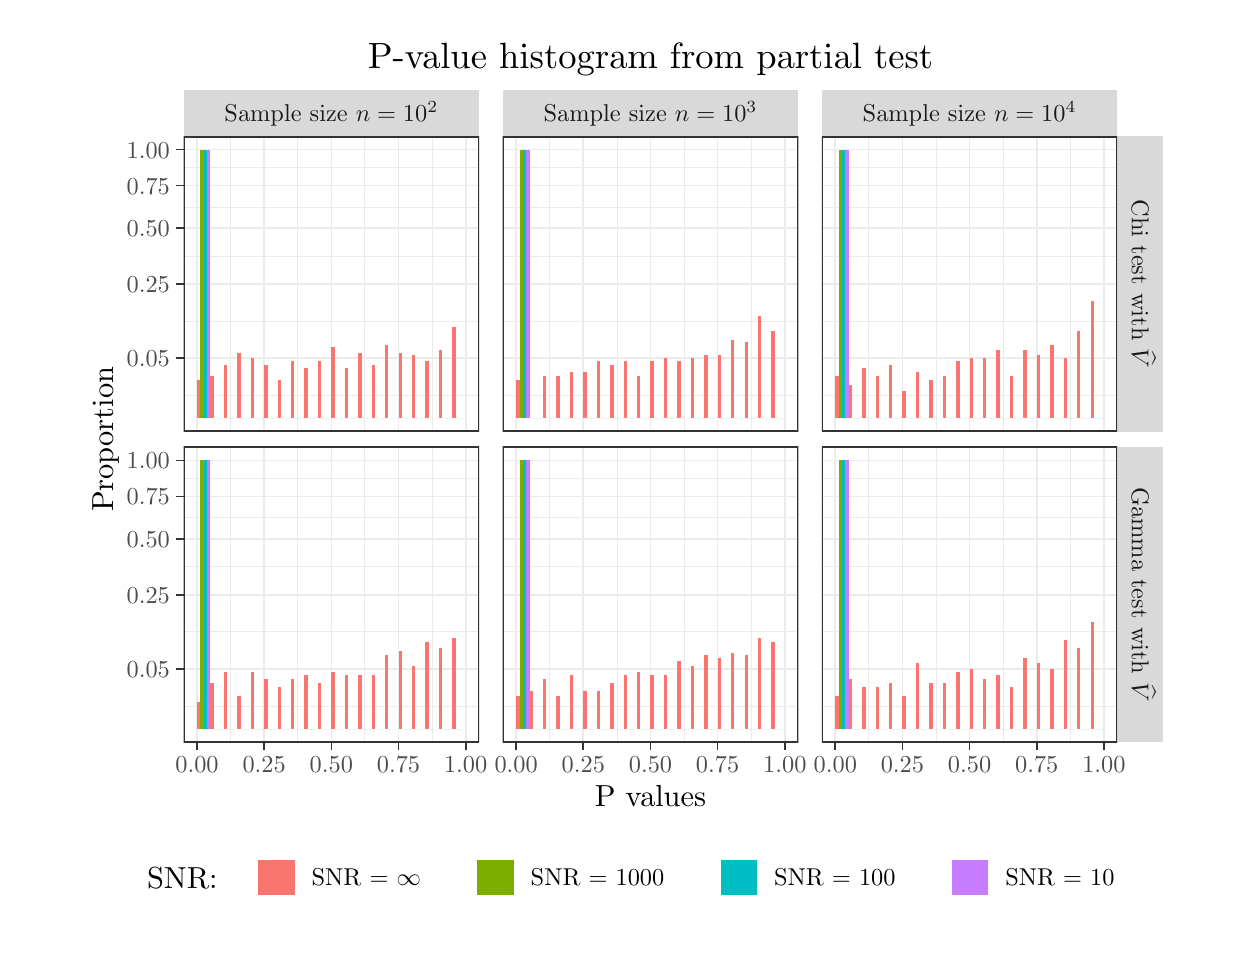
\begin{tikzpicture}[x=1pt,y=1pt]
\definecolor{fillColor}{RGB}{255,255,255}
\path[use as bounding box,fill=fillColor,fill opacity=0.00] (0,0) rectangle (433.62,325.21);
\begin{scope}
\path[clip] ( 17.78,  0.00) rectangle (415.84,325.21);
\definecolor{drawColor}{RGB}{255,255,255}
\definecolor{fillColor}{RGB}{255,255,255}

\path[draw=drawColor,line width= 0.6pt,line join=round,line cap=round,fill=fillColor] ( 17.78,  0.00) rectangle (415.84,325.21);
\end{scope}
\begin{scope}
\path[clip] ( 56.34,179.20) rectangle (163.12,285.99);
\definecolor{fillColor}{RGB}{255,255,255}

\path[fill=fillColor] ( 56.34,179.20) rectangle (163.12,285.99);
\definecolor{drawColor}{gray}{0.92}

\path[draw=drawColor,line width= 0.3pt,line join=round] ( 56.34,192.34) --
	(163.12,192.34);

\path[draw=drawColor,line width= 0.3pt,line join=round] ( 56.34,219.18) --
	(163.12,219.18);

\path[draw=drawColor,line width= 0.3pt,line join=round] ( 56.34,242.65) --
	(163.12,242.65);

\path[draw=drawColor,line width= 0.3pt,line join=round] ( 56.34,260.41) --
	(163.12,260.41);

\path[draw=drawColor,line width= 0.3pt,line join=round] ( 56.34,274.63) --
	(163.12,274.63);

\path[draw=drawColor,line width= 0.3pt,line join=round] ( 73.32,179.20) --
	( 73.32,285.99);

\path[draw=drawColor,line width= 0.3pt,line join=round] ( 97.59,179.20) --
	( 97.59,285.99);

\path[draw=drawColor,line width= 0.3pt,line join=round] (121.86,179.20) --
	(121.86,285.99);

\path[draw=drawColor,line width= 0.3pt,line join=round] (146.13,179.20) --
	(146.13,285.99);

\path[draw=drawColor,line width= 0.6pt,line join=round] ( 56.34,205.76) --
	(163.12,205.76);

\path[draw=drawColor,line width= 0.6pt,line join=round] ( 56.34,232.59) --
	(163.12,232.59);

\path[draw=drawColor,line width= 0.6pt,line join=round] ( 56.34,252.70) --
	(163.12,252.70);

\path[draw=drawColor,line width= 0.6pt,line join=round] ( 56.34,268.13) --
	(163.12,268.13);

\path[draw=drawColor,line width= 0.6pt,line join=round] ( 56.34,281.13) --
	(163.12,281.13);

\path[draw=drawColor,line width= 0.6pt,line join=round] ( 61.19,179.20) --
	( 61.19,285.99);

\path[draw=drawColor,line width= 0.6pt,line join=round] ( 85.46,179.20) --
	( 85.46,285.99);

\path[draw=drawColor,line width= 0.6pt,line join=round] (109.73,179.20) --
	(109.73,285.99);

\path[draw=drawColor,line width= 0.6pt,line join=round] (134.00,179.20) --
	(134.00,285.99);

\path[draw=drawColor,line width= 0.6pt,line join=round] (158.27,179.20) --
	(158.27,285.99);
\definecolor{fillColor}{RGB}{248,118,109}

\path[fill=fillColor] ( 61.19,184.05) rectangle ( 62.40,197.78);

\path[fill=fillColor] ( 66.04,184.05) rectangle ( 67.26,199.40);

\path[fill=fillColor] ( 70.90,184.05) rectangle ( 72.11,203.47);

\path[fill=fillColor] ( 75.75,184.05) rectangle ( 76.96,207.83);

\path[fill=fillColor] ( 80.61,184.05) rectangle ( 81.82,205.76);

\path[fill=fillColor] ( 85.46,184.05) rectangle ( 86.67,203.47);

\path[fill=fillColor] ( 90.31,184.05) rectangle ( 91.53,197.78);

\path[fill=fillColor] ( 95.17,184.05) rectangle ( 96.38,204.65);

\path[fill=fillColor] (100.02,184.05) rectangle (101.23,202.22);

\path[fill=fillColor] (104.87,184.05) rectangle (106.09,204.65);

\path[fill=fillColor] (109.73,184.05) rectangle (110.94,209.74);

\path[fill=fillColor] (114.58,184.05) rectangle (115.80,202.22);

\path[fill=fillColor] (119.44,184.05) rectangle (120.65,207.83);

\path[fill=fillColor] (124.29,184.05) rectangle (125.50,203.47);

\path[fill=fillColor] (129.14,184.05) rectangle (130.36,210.64);

\path[fill=fillColor] (134.00,184.05) rectangle (135.21,207.83);

\path[fill=fillColor] (138.85,184.05) rectangle (140.07,206.82);

\path[fill=fillColor] (143.71,184.05) rectangle (144.92,204.65);

\path[fill=fillColor] (148.56,184.05) rectangle (149.77,208.80);

\path[fill=fillColor] (153.41,184.05) rectangle (154.63,216.97);
\definecolor{fillColor}{RGB}{124,174,0}

\path[fill=fillColor] ( 62.40,184.05) rectangle ( 63.62,281.13);

\path[fill=fillColor] ( 67.26,184.05) rectangle ( 68.47,184.05);

\path[fill=fillColor] ( 72.11,184.05) rectangle ( 73.32,184.05);

\path[fill=fillColor] ( 76.96,184.05) rectangle ( 78.18,184.05);

\path[fill=fillColor] ( 81.82,184.05) rectangle ( 83.03,184.05);

\path[fill=fillColor] ( 86.67,184.05) rectangle ( 87.89,184.05);

\path[fill=fillColor] ( 91.53,184.05) rectangle ( 92.74,184.05);

\path[fill=fillColor] ( 96.38,184.05) rectangle ( 97.59,184.05);

\path[fill=fillColor] (101.23,184.05) rectangle (102.45,184.05);

\path[fill=fillColor] (106.09,184.05) rectangle (107.30,184.05);

\path[fill=fillColor] (110.94,184.05) rectangle (112.16,184.05);

\path[fill=fillColor] (115.80,184.05) rectangle (117.01,184.05);

\path[fill=fillColor] (120.65,184.05) rectangle (121.86,184.05);

\path[fill=fillColor] (125.50,184.05) rectangle (126.72,184.05);

\path[fill=fillColor] (130.36,184.05) rectangle (131.57,184.05);

\path[fill=fillColor] (135.21,184.05) rectangle (136.43,184.05);

\path[fill=fillColor] (140.07,184.05) rectangle (141.28,184.05);

\path[fill=fillColor] (144.92,184.05) rectangle (146.13,184.05);

\path[fill=fillColor] (149.77,184.05) rectangle (150.99,184.05);

\path[fill=fillColor] (154.63,184.05) rectangle (155.84,184.05);
\definecolor{fillColor}{RGB}{0,191,196}

\path[fill=fillColor] ( 63.62,184.05) rectangle ( 64.83,281.13);

\path[fill=fillColor] ( 68.47,184.05) rectangle ( 69.68,184.05);

\path[fill=fillColor] ( 73.32,184.05) rectangle ( 74.54,184.05);

\path[fill=fillColor] ( 78.18,184.05) rectangle ( 79.39,184.05);

\path[fill=fillColor] ( 83.03,184.05) rectangle ( 84.25,184.05);

\path[fill=fillColor] ( 87.89,184.05) rectangle ( 89.10,184.05);

\path[fill=fillColor] ( 92.74,184.05) rectangle ( 93.95,184.05);

\path[fill=fillColor] ( 97.59,184.05) rectangle ( 98.81,184.05);

\path[fill=fillColor] (102.45,184.05) rectangle (103.66,184.05);

\path[fill=fillColor] (107.30,184.05) rectangle (108.52,184.05);

\path[fill=fillColor] (112.16,184.05) rectangle (113.37,184.05);

\path[fill=fillColor] (117.01,184.05) rectangle (118.22,184.05);

\path[fill=fillColor] (121.86,184.05) rectangle (123.08,184.05);

\path[fill=fillColor] (126.72,184.05) rectangle (127.93,184.05);

\path[fill=fillColor] (131.57,184.05) rectangle (132.79,184.05);

\path[fill=fillColor] (136.43,184.05) rectangle (137.64,184.05);

\path[fill=fillColor] (141.28,184.05) rectangle (142.49,184.05);

\path[fill=fillColor] (146.13,184.05) rectangle (147.35,184.05);

\path[fill=fillColor] (150.99,184.05) rectangle (152.20,184.05);

\path[fill=fillColor] (155.84,184.05) rectangle (157.05,184.05);
\definecolor{fillColor}{RGB}{199,124,255}

\path[fill=fillColor] ( 64.83,184.05) rectangle ( 66.04,281.13);

\path[fill=fillColor] ( 69.68,184.05) rectangle ( 70.90,184.05);

\path[fill=fillColor] ( 74.54,184.05) rectangle ( 75.75,184.05);

\path[fill=fillColor] ( 79.39,184.05) rectangle ( 80.61,184.05);

\path[fill=fillColor] ( 84.25,184.05) rectangle ( 85.46,184.05);

\path[fill=fillColor] ( 89.10,184.05) rectangle ( 90.31,184.05);

\path[fill=fillColor] ( 93.95,184.05) rectangle ( 95.17,184.05);

\path[fill=fillColor] ( 98.81,184.05) rectangle (100.02,184.05);

\path[fill=fillColor] (103.66,184.05) rectangle (104.87,184.05);

\path[fill=fillColor] (108.52,184.05) rectangle (109.73,184.05);

\path[fill=fillColor] (113.37,184.05) rectangle (114.58,184.05);

\path[fill=fillColor] (118.22,184.05) rectangle (119.44,184.05);

\path[fill=fillColor] (123.08,184.05) rectangle (124.29,184.05);

\path[fill=fillColor] (127.93,184.05) rectangle (129.14,184.05);

\path[fill=fillColor] (132.79,184.05) rectangle (134.00,184.05);

\path[fill=fillColor] (137.64,184.05) rectangle (138.85,184.05);

\path[fill=fillColor] (142.49,184.05) rectangle (143.71,184.05);

\path[fill=fillColor] (147.35,184.05) rectangle (148.56,184.05);

\path[fill=fillColor] (152.20,184.05) rectangle (153.41,184.05);

\path[fill=fillColor] (157.05,184.05) rectangle (158.27,184.05);
\definecolor{drawColor}{gray}{0.20}

\path[draw=drawColor,line width= 1.1pt,line join=round,line cap=round] ( 56.34,179.20) rectangle (163.12,285.99);
\end{scope}
\begin{scope}
\path[clip] ( 56.34, 66.91) rectangle (163.12,173.70);
\definecolor{fillColor}{RGB}{255,255,255}

\path[fill=fillColor] ( 56.34, 66.91) rectangle (163.12,173.70);
\definecolor{drawColor}{gray}{0.92}

\path[draw=drawColor,line width= 0.3pt,line join=round] ( 56.34, 80.06) --
	(163.12, 80.06);

\path[draw=drawColor,line width= 0.3pt,line join=round] ( 56.34,106.89) --
	(163.12,106.89);

\path[draw=drawColor,line width= 0.3pt,line join=round] ( 56.34,130.36) --
	(163.12,130.36);

\path[draw=drawColor,line width= 0.3pt,line join=round] ( 56.34,148.13) --
	(163.12,148.13);

\path[draw=drawColor,line width= 0.3pt,line join=round] ( 56.34,162.34) --
	(163.12,162.34);

\path[draw=drawColor,line width= 0.3pt,line join=round] ( 73.32, 66.91) --
	( 73.32,173.70);

\path[draw=drawColor,line width= 0.3pt,line join=round] ( 97.59, 66.91) --
	( 97.59,173.70);

\path[draw=drawColor,line width= 0.3pt,line join=round] (121.86, 66.91) --
	(121.86,173.70);

\path[draw=drawColor,line width= 0.3pt,line join=round] (146.13, 66.91) --
	(146.13,173.70);

\path[draw=drawColor,line width= 0.6pt,line join=round] ( 56.34, 93.47) --
	(163.12, 93.47);

\path[draw=drawColor,line width= 0.6pt,line join=round] ( 56.34,120.31) --
	(163.12,120.31);

\path[draw=drawColor,line width= 0.6pt,line join=round] ( 56.34,140.41) --
	(163.12,140.41);

\path[draw=drawColor,line width= 0.6pt,line join=round] ( 56.34,155.84) --
	(163.12,155.84);

\path[draw=drawColor,line width= 0.6pt,line join=round] ( 56.34,168.85) --
	(163.12,168.85);

\path[draw=drawColor,line width= 0.6pt,line join=round] ( 61.19, 66.91) --
	( 61.19,173.70);

\path[draw=drawColor,line width= 0.6pt,line join=round] ( 85.46, 66.91) --
	( 85.46,173.70);

\path[draw=drawColor,line width= 0.6pt,line join=round] (109.73, 66.91) --
	(109.73,173.70);

\path[draw=drawColor,line width= 0.6pt,line join=round] (134.00, 66.91) --
	(134.00,173.70);

\path[draw=drawColor,line width= 0.6pt,line join=round] (158.27, 66.91) --
	(158.27,173.70);
\definecolor{fillColor}{RGB}{248,118,109}

\path[fill=fillColor] ( 61.19, 71.77) rectangle ( 62.40, 81.47);

\path[fill=fillColor] ( 66.04, 71.77) rectangle ( 67.26, 88.58);

\path[fill=fillColor] ( 70.90, 71.77) rectangle ( 72.11, 92.36);

\path[fill=fillColor] ( 75.75, 71.77) rectangle ( 76.96, 83.66);

\path[fill=fillColor] ( 80.61, 71.77) rectangle ( 81.82, 92.36);

\path[fill=fillColor] ( 85.46, 71.77) rectangle ( 86.67, 89.93);

\path[fill=fillColor] ( 90.31, 71.77) rectangle ( 91.53, 87.12);

\path[fill=fillColor] ( 95.17, 71.77) rectangle ( 96.38, 89.93);

\path[fill=fillColor] (100.02, 71.77) rectangle (101.23, 91.18);

\path[fill=fillColor] (104.87, 71.77) rectangle (106.09, 88.58);

\path[fill=fillColor] (109.73, 71.77) rectangle (110.94, 92.36);

\path[fill=fillColor] (114.58, 71.77) rectangle (115.80, 91.18);

\path[fill=fillColor] (119.44, 71.77) rectangle (120.65, 91.18);

\path[fill=fillColor] (124.29, 71.77) rectangle (125.50, 91.18);

\path[fill=fillColor] (129.14, 71.77) rectangle (130.36, 98.35);

\path[fill=fillColor] (134.00, 71.77) rectangle (135.21,100.07);

\path[fill=fillColor] (138.85, 71.77) rectangle (140.07, 94.53);

\path[fill=fillColor] (143.71, 71.77) rectangle (144.92,103.22);

\path[fill=fillColor] (148.56, 71.77) rectangle (149.77,100.89);

\path[fill=fillColor] (153.41, 71.77) rectangle (154.63,104.69);
\definecolor{fillColor}{RGB}{124,174,0}

\path[fill=fillColor] ( 62.40, 71.77) rectangle ( 63.62,168.85);

\path[fill=fillColor] ( 67.26, 71.77) rectangle ( 68.47, 71.77);

\path[fill=fillColor] ( 72.11, 71.77) rectangle ( 73.32, 71.77);

\path[fill=fillColor] ( 76.96, 71.77) rectangle ( 78.18, 71.77);

\path[fill=fillColor] ( 81.82, 71.77) rectangle ( 83.03, 71.77);

\path[fill=fillColor] ( 86.67, 71.77) rectangle ( 87.89, 71.77);

\path[fill=fillColor] ( 91.53, 71.77) rectangle ( 92.74, 71.77);

\path[fill=fillColor] ( 96.38, 71.77) rectangle ( 97.59, 71.77);

\path[fill=fillColor] (101.23, 71.77) rectangle (102.45, 71.77);

\path[fill=fillColor] (106.09, 71.77) rectangle (107.30, 71.77);

\path[fill=fillColor] (110.94, 71.77) rectangle (112.16, 71.77);

\path[fill=fillColor] (115.80, 71.77) rectangle (117.01, 71.77);

\path[fill=fillColor] (120.65, 71.77) rectangle (121.86, 71.77);

\path[fill=fillColor] (125.50, 71.77) rectangle (126.72, 71.77);

\path[fill=fillColor] (130.36, 71.77) rectangle (131.57, 71.77);

\path[fill=fillColor] (135.21, 71.77) rectangle (136.43, 71.77);

\path[fill=fillColor] (140.07, 71.77) rectangle (141.28, 71.77);

\path[fill=fillColor] (144.92, 71.77) rectangle (146.13, 71.77);

\path[fill=fillColor] (149.77, 71.77) rectangle (150.99, 71.77);

\path[fill=fillColor] (154.63, 71.77) rectangle (155.84, 71.77);
\definecolor{fillColor}{RGB}{0,191,196}

\path[fill=fillColor] ( 63.62, 71.77) rectangle ( 64.83,168.85);

\path[fill=fillColor] ( 68.47, 71.77) rectangle ( 69.68, 71.77);

\path[fill=fillColor] ( 73.32, 71.77) rectangle ( 74.54, 71.77);

\path[fill=fillColor] ( 78.18, 71.77) rectangle ( 79.39, 71.77);

\path[fill=fillColor] ( 83.03, 71.77) rectangle ( 84.25, 71.77);

\path[fill=fillColor] ( 87.89, 71.77) rectangle ( 89.10, 71.77);

\path[fill=fillColor] ( 92.74, 71.77) rectangle ( 93.95, 71.77);

\path[fill=fillColor] ( 97.59, 71.77) rectangle ( 98.81, 71.77);

\path[fill=fillColor] (102.45, 71.77) rectangle (103.66, 71.77);

\path[fill=fillColor] (107.30, 71.77) rectangle (108.52, 71.77);

\path[fill=fillColor] (112.16, 71.77) rectangle (113.37, 71.77);

\path[fill=fillColor] (117.01, 71.77) rectangle (118.22, 71.77);

\path[fill=fillColor] (121.86, 71.77) rectangle (123.08, 71.77);

\path[fill=fillColor] (126.72, 71.77) rectangle (127.93, 71.77);

\path[fill=fillColor] (131.57, 71.77) rectangle (132.79, 71.77);

\path[fill=fillColor] (136.43, 71.77) rectangle (137.64, 71.77);

\path[fill=fillColor] (141.28, 71.77) rectangle (142.49, 71.77);

\path[fill=fillColor] (146.13, 71.77) rectangle (147.35, 71.77);

\path[fill=fillColor] (150.99, 71.77) rectangle (152.20, 71.77);

\path[fill=fillColor] (155.84, 71.77) rectangle (157.05, 71.77);
\definecolor{fillColor}{RGB}{199,124,255}

\path[fill=fillColor] ( 64.83, 71.77) rectangle ( 66.04,168.85);

\path[fill=fillColor] ( 69.68, 71.77) rectangle ( 70.90, 71.77);

\path[fill=fillColor] ( 74.54, 71.77) rectangle ( 75.75, 71.77);

\path[fill=fillColor] ( 79.39, 71.77) rectangle ( 80.61, 71.77);

\path[fill=fillColor] ( 84.25, 71.77) rectangle ( 85.46, 71.77);

\path[fill=fillColor] ( 89.10, 71.77) rectangle ( 90.31, 71.77);

\path[fill=fillColor] ( 93.95, 71.77) rectangle ( 95.17, 71.77);

\path[fill=fillColor] ( 98.81, 71.77) rectangle (100.02, 71.77);

\path[fill=fillColor] (103.66, 71.77) rectangle (104.87, 71.77);

\path[fill=fillColor] (108.52, 71.77) rectangle (109.73, 71.77);

\path[fill=fillColor] (113.37, 71.77) rectangle (114.58, 71.77);

\path[fill=fillColor] (118.22, 71.77) rectangle (119.44, 71.77);

\path[fill=fillColor] (123.08, 71.77) rectangle (124.29, 71.77);

\path[fill=fillColor] (127.93, 71.77) rectangle (129.14, 71.77);

\path[fill=fillColor] (132.79, 71.77) rectangle (134.00, 71.77);

\path[fill=fillColor] (137.64, 71.77) rectangle (138.85, 71.77);

\path[fill=fillColor] (142.49, 71.77) rectangle (143.71, 71.77);

\path[fill=fillColor] (147.35, 71.77) rectangle (148.56, 71.77);

\path[fill=fillColor] (152.20, 71.77) rectangle (153.41, 71.77);

\path[fill=fillColor] (157.05, 71.77) rectangle (158.27, 71.77);
\definecolor{drawColor}{gray}{0.20}

\path[draw=drawColor,line width= 1.1pt,line join=round,line cap=round] ( 56.34, 66.91) rectangle (163.12,173.70);
\end{scope}
\begin{scope}
\path[clip] (171.66,179.20) rectangle (278.45,285.99);
\definecolor{fillColor}{RGB}{255,255,255}

\path[fill=fillColor] (171.66,179.20) rectangle (278.45,285.99);
\definecolor{drawColor}{gray}{0.92}

\path[draw=drawColor,line width= 0.3pt,line join=round] (171.66,192.34) --
	(278.45,192.34);

\path[draw=drawColor,line width= 0.3pt,line join=round] (171.66,219.18) --
	(278.45,219.18);

\path[draw=drawColor,line width= 0.3pt,line join=round] (171.66,242.65) --
	(278.45,242.65);

\path[draw=drawColor,line width= 0.3pt,line join=round] (171.66,260.41) --
	(278.45,260.41);

\path[draw=drawColor,line width= 0.3pt,line join=round] (171.66,274.63) --
	(278.45,274.63);

\path[draw=drawColor,line width= 0.3pt,line join=round] (188.65,179.20) --
	(188.65,285.99);

\path[draw=drawColor,line width= 0.3pt,line join=round] (212.92,179.20) --
	(212.92,285.99);

\path[draw=drawColor,line width= 0.3pt,line join=round] (237.19,179.20) --
	(237.19,285.99);

\path[draw=drawColor,line width= 0.3pt,line join=round] (261.46,179.20) --
	(261.46,285.99);

\path[draw=drawColor,line width= 0.6pt,line join=round] (171.66,205.76) --
	(278.45,205.76);

\path[draw=drawColor,line width= 0.6pt,line join=round] (171.66,232.59) --
	(278.45,232.59);

\path[draw=drawColor,line width= 0.6pt,line join=round] (171.66,252.70) --
	(278.45,252.70);

\path[draw=drawColor,line width= 0.6pt,line join=round] (171.66,268.13) --
	(278.45,268.13);

\path[draw=drawColor,line width= 0.6pt,line join=round] (171.66,281.13) --
	(278.45,281.13);

\path[draw=drawColor,line width= 0.6pt,line join=round] (176.51,179.20) --
	(176.51,285.99);

\path[draw=drawColor,line width= 0.6pt,line join=round] (200.78,179.20) --
	(200.78,285.99);

\path[draw=drawColor,line width= 0.6pt,line join=round] (225.05,179.20) --
	(225.05,285.99);

\path[draw=drawColor,line width= 0.6pt,line join=round] (249.32,179.20) --
	(249.32,285.99);

\path[draw=drawColor,line width= 0.6pt,line join=round] (273.59,179.20) --
	(273.59,285.99);
\definecolor{fillColor}{RGB}{248,118,109}

\path[fill=fillColor] (176.51,184.05) rectangle (177.73,197.78);

\path[fill=fillColor] (181.37,184.05) rectangle (182.58,184.05);

\path[fill=fillColor] (186.22,184.05) rectangle (187.43,199.40);

\path[fill=fillColor] (191.07,184.05) rectangle (192.29,199.40);

\path[fill=fillColor] (195.93,184.05) rectangle (197.14,200.87);

\path[fill=fillColor] (200.78,184.05) rectangle (202.00,200.87);

\path[fill=fillColor] (205.64,184.05) rectangle (206.85,204.65);

\path[fill=fillColor] (210.49,184.05) rectangle (211.70,203.47);

\path[fill=fillColor] (215.34,184.05) rectangle (216.56,204.65);

\path[fill=fillColor] (220.20,184.05) rectangle (221.41,199.40);

\path[fill=fillColor] (225.05,184.05) rectangle (226.27,204.65);

\path[fill=fillColor] (229.91,184.05) rectangle (231.12,205.76);

\path[fill=fillColor] (234.76,184.05) rectangle (235.97,204.65);

\path[fill=fillColor] (239.61,184.05) rectangle (240.83,205.76);

\path[fill=fillColor] (244.47,184.05) rectangle (245.68,206.82);

\path[fill=fillColor] (249.32,184.05) rectangle (250.54,206.82);

\path[fill=fillColor] (254.18,184.05) rectangle (255.39,212.36);

\path[fill=fillColor] (259.03,184.05) rectangle (260.24,211.51);

\path[fill=fillColor] (263.88,184.05) rectangle (265.10,221.02);

\path[fill=fillColor] (268.74,184.05) rectangle (269.95,215.51);
\definecolor{fillColor}{RGB}{124,174,0}

\path[fill=fillColor] (177.73,184.05) rectangle (178.94,281.13);

\path[fill=fillColor] (182.58,184.05) rectangle (183.79,184.05);

\path[fill=fillColor] (187.43,184.05) rectangle (188.65,184.05);

\path[fill=fillColor] (192.29,184.05) rectangle (193.50,184.05);

\path[fill=fillColor] (197.14,184.05) rectangle (198.36,184.05);

\path[fill=fillColor] (202.00,184.05) rectangle (203.21,184.05);

\path[fill=fillColor] (206.85,184.05) rectangle (208.06,184.05);

\path[fill=fillColor] (211.70,184.05) rectangle (212.92,184.05);

\path[fill=fillColor] (216.56,184.05) rectangle (217.77,184.05);

\path[fill=fillColor] (221.41,184.05) rectangle (222.62,184.05);

\path[fill=fillColor] (226.27,184.05) rectangle (227.48,184.05);

\path[fill=fillColor] (231.12,184.05) rectangle (232.33,184.05);

\path[fill=fillColor] (235.97,184.05) rectangle (237.19,184.05);

\path[fill=fillColor] (240.83,184.05) rectangle (242.04,184.05);

\path[fill=fillColor] (245.68,184.05) rectangle (246.89,184.05);

\path[fill=fillColor] (250.54,184.05) rectangle (251.75,184.05);

\path[fill=fillColor] (255.39,184.05) rectangle (256.60,184.05);

\path[fill=fillColor] (260.24,184.05) rectangle (261.46,184.05);

\path[fill=fillColor] (265.10,184.05) rectangle (266.31,184.05);

\path[fill=fillColor] (269.95,184.05) rectangle (271.16,184.05);
\definecolor{fillColor}{RGB}{0,191,196}

\path[fill=fillColor] (178.94,184.05) rectangle (180.15,281.13);

\path[fill=fillColor] (183.79,184.05) rectangle (185.01,184.05);

\path[fill=fillColor] (188.65,184.05) rectangle (189.86,184.05);

\path[fill=fillColor] (193.50,184.05) rectangle (194.71,184.05);

\path[fill=fillColor] (198.36,184.05) rectangle (199.57,184.05);

\path[fill=fillColor] (203.21,184.05) rectangle (204.42,184.05);

\path[fill=fillColor] (208.06,184.05) rectangle (209.28,184.05);

\path[fill=fillColor] (212.92,184.05) rectangle (214.13,184.05);

\path[fill=fillColor] (217.77,184.05) rectangle (218.98,184.05);

\path[fill=fillColor] (222.62,184.05) rectangle (223.84,184.05);

\path[fill=fillColor] (227.48,184.05) rectangle (228.69,184.05);

\path[fill=fillColor] (232.33,184.05) rectangle (233.55,184.05);

\path[fill=fillColor] (237.19,184.05) rectangle (238.40,184.05);

\path[fill=fillColor] (242.04,184.05) rectangle (243.25,184.05);

\path[fill=fillColor] (246.89,184.05) rectangle (248.11,184.05);

\path[fill=fillColor] (251.75,184.05) rectangle (252.96,184.05);

\path[fill=fillColor] (256.60,184.05) rectangle (257.82,184.05);

\path[fill=fillColor] (261.46,184.05) rectangle (262.67,184.05);

\path[fill=fillColor] (266.31,184.05) rectangle (267.52,184.05);

\path[fill=fillColor] (271.16,184.05) rectangle (272.38,184.05);
\definecolor{fillColor}{RGB}{199,124,255}

\path[fill=fillColor] (180.15,184.05) rectangle (181.37,281.13);

\path[fill=fillColor] (185.01,184.05) rectangle (186.22,184.05);

\path[fill=fillColor] (189.86,184.05) rectangle (191.07,184.05);

\path[fill=fillColor] (194.71,184.05) rectangle (195.93,184.05);

\path[fill=fillColor] (199.57,184.05) rectangle (200.78,184.05);

\path[fill=fillColor] (204.42,184.05) rectangle (205.64,184.05);

\path[fill=fillColor] (209.28,184.05) rectangle (210.49,184.05);

\path[fill=fillColor] (214.13,184.05) rectangle (215.34,184.05);

\path[fill=fillColor] (218.98,184.05) rectangle (220.20,184.05);

\path[fill=fillColor] (223.84,184.05) rectangle (225.05,184.05);

\path[fill=fillColor] (228.69,184.05) rectangle (229.91,184.05);

\path[fill=fillColor] (233.55,184.05) rectangle (234.76,184.05);

\path[fill=fillColor] (238.40,184.05) rectangle (239.61,184.05);

\path[fill=fillColor] (243.25,184.05) rectangle (244.47,184.05);

\path[fill=fillColor] (248.11,184.05) rectangle (249.32,184.05);

\path[fill=fillColor] (252.96,184.05) rectangle (254.18,184.05);

\path[fill=fillColor] (257.82,184.05) rectangle (259.03,184.05);

\path[fill=fillColor] (262.67,184.05) rectangle (263.88,184.05);

\path[fill=fillColor] (267.52,184.05) rectangle (268.74,184.05);

\path[fill=fillColor] (272.38,184.05) rectangle (273.59,184.05);
\definecolor{drawColor}{gray}{0.20}

\path[draw=drawColor,line width= 1.1pt,line join=round,line cap=round] (171.66,179.20) rectangle (278.45,285.99);
\end{scope}
\begin{scope}
\path[clip] (171.66, 66.91) rectangle (278.45,173.70);
\definecolor{fillColor}{RGB}{255,255,255}

\path[fill=fillColor] (171.66, 66.91) rectangle (278.45,173.70);
\definecolor{drawColor}{gray}{0.92}

\path[draw=drawColor,line width= 0.3pt,line join=round] (171.66, 80.06) --
	(278.45, 80.06);

\path[draw=drawColor,line width= 0.3pt,line join=round] (171.66,106.89) --
	(278.45,106.89);

\path[draw=drawColor,line width= 0.3pt,line join=round] (171.66,130.36) --
	(278.45,130.36);

\path[draw=drawColor,line width= 0.3pt,line join=round] (171.66,148.13) --
	(278.45,148.13);

\path[draw=drawColor,line width= 0.3pt,line join=round] (171.66,162.34) --
	(278.45,162.34);

\path[draw=drawColor,line width= 0.3pt,line join=round] (188.65, 66.91) --
	(188.65,173.70);

\path[draw=drawColor,line width= 0.3pt,line join=round] (212.92, 66.91) --
	(212.92,173.70);

\path[draw=drawColor,line width= 0.3pt,line join=round] (237.19, 66.91) --
	(237.19,173.70);

\path[draw=drawColor,line width= 0.3pt,line join=round] (261.46, 66.91) --
	(261.46,173.70);

\path[draw=drawColor,line width= 0.6pt,line join=round] (171.66, 93.47) --
	(278.45, 93.47);

\path[draw=drawColor,line width= 0.6pt,line join=round] (171.66,120.31) --
	(278.45,120.31);

\path[draw=drawColor,line width= 0.6pt,line join=round] (171.66,140.41) --
	(278.45,140.41);

\path[draw=drawColor,line width= 0.6pt,line join=round] (171.66,155.84) --
	(278.45,155.84);

\path[draw=drawColor,line width= 0.6pt,line join=round] (171.66,168.85) --
	(278.45,168.85);

\path[draw=drawColor,line width= 0.6pt,line join=round] (176.51, 66.91) --
	(176.51,173.70);

\path[draw=drawColor,line width= 0.6pt,line join=round] (200.78, 66.91) --
	(200.78,173.70);

\path[draw=drawColor,line width= 0.6pt,line join=round] (225.05, 66.91) --
	(225.05,173.70);

\path[draw=drawColor,line width= 0.6pt,line join=round] (249.32, 66.91) --
	(249.32,173.70);

\path[draw=drawColor,line width= 0.6pt,line join=round] (273.59, 66.91) --
	(273.59,173.70);
\definecolor{fillColor}{RGB}{248,118,109}

\path[fill=fillColor] (176.51, 71.77) rectangle (177.73, 83.66);

\path[fill=fillColor] (181.37, 71.77) rectangle (182.58, 85.50);

\path[fill=fillColor] (186.22, 71.77) rectangle (187.43, 89.93);

\path[fill=fillColor] (191.07, 71.77) rectangle (192.29, 83.66);

\path[fill=fillColor] (195.93, 71.77) rectangle (197.14, 91.18);

\path[fill=fillColor] (200.78, 71.77) rectangle (202.00, 85.50);

\path[fill=fillColor] (205.64, 71.77) rectangle (206.85, 85.50);

\path[fill=fillColor] (210.49, 71.77) rectangle (211.70, 88.58);

\path[fill=fillColor] (215.34, 71.77) rectangle (216.56, 91.18);

\path[fill=fillColor] (220.20, 71.77) rectangle (221.41, 92.36);

\path[fill=fillColor] (225.05, 71.77) rectangle (226.27, 91.18);

\path[fill=fillColor] (229.91, 71.77) rectangle (231.12, 91.18);

\path[fill=fillColor] (234.76, 71.77) rectangle (235.97, 96.52);

\path[fill=fillColor] (239.61, 71.77) rectangle (240.83, 94.53);

\path[fill=fillColor] (244.47, 71.77) rectangle (245.68, 98.35);

\path[fill=fillColor] (249.32, 71.77) rectangle (250.54, 97.45);

\path[fill=fillColor] (254.18, 71.77) rectangle (255.39, 99.22);

\path[fill=fillColor] (259.03, 71.77) rectangle (260.24, 98.35);

\path[fill=fillColor] (263.88, 71.77) rectangle (265.10,104.69);

\path[fill=fillColor] (268.74, 71.77) rectangle (269.95,103.22);
\definecolor{fillColor}{RGB}{124,174,0}

\path[fill=fillColor] (177.73, 71.77) rectangle (178.94,168.85);

\path[fill=fillColor] (182.58, 71.77) rectangle (183.79, 71.77);

\path[fill=fillColor] (187.43, 71.77) rectangle (188.65, 71.77);

\path[fill=fillColor] (192.29, 71.77) rectangle (193.50, 71.77);

\path[fill=fillColor] (197.14, 71.77) rectangle (198.36, 71.77);

\path[fill=fillColor] (202.00, 71.77) rectangle (203.21, 71.77);

\path[fill=fillColor] (206.85, 71.77) rectangle (208.06, 71.77);

\path[fill=fillColor] (211.70, 71.77) rectangle (212.92, 71.77);

\path[fill=fillColor] (216.56, 71.77) rectangle (217.77, 71.77);

\path[fill=fillColor] (221.41, 71.77) rectangle (222.62, 71.77);

\path[fill=fillColor] (226.27, 71.77) rectangle (227.48, 71.77);

\path[fill=fillColor] (231.12, 71.77) rectangle (232.33, 71.77);

\path[fill=fillColor] (235.97, 71.77) rectangle (237.19, 71.77);

\path[fill=fillColor] (240.83, 71.77) rectangle (242.04, 71.77);

\path[fill=fillColor] (245.68, 71.77) rectangle (246.89, 71.77);

\path[fill=fillColor] (250.54, 71.77) rectangle (251.75, 71.77);

\path[fill=fillColor] (255.39, 71.77) rectangle (256.60, 71.77);

\path[fill=fillColor] (260.24, 71.77) rectangle (261.46, 71.77);

\path[fill=fillColor] (265.10, 71.77) rectangle (266.31, 71.77);

\path[fill=fillColor] (269.95, 71.77) rectangle (271.16, 71.77);
\definecolor{fillColor}{RGB}{0,191,196}

\path[fill=fillColor] (178.94, 71.77) rectangle (180.15,168.85);

\path[fill=fillColor] (183.79, 71.77) rectangle (185.01, 71.77);

\path[fill=fillColor] (188.65, 71.77) rectangle (189.86, 71.77);

\path[fill=fillColor] (193.50, 71.77) rectangle (194.71, 71.77);

\path[fill=fillColor] (198.36, 71.77) rectangle (199.57, 71.77);

\path[fill=fillColor] (203.21, 71.77) rectangle (204.42, 71.77);

\path[fill=fillColor] (208.06, 71.77) rectangle (209.28, 71.77);

\path[fill=fillColor] (212.92, 71.77) rectangle (214.13, 71.77);

\path[fill=fillColor] (217.77, 71.77) rectangle (218.98, 71.77);

\path[fill=fillColor] (222.62, 71.77) rectangle (223.84, 71.77);

\path[fill=fillColor] (227.48, 71.77) rectangle (228.69, 71.77);

\path[fill=fillColor] (232.33, 71.77) rectangle (233.55, 71.77);

\path[fill=fillColor] (237.19, 71.77) rectangle (238.40, 71.77);

\path[fill=fillColor] (242.04, 71.77) rectangle (243.25, 71.77);

\path[fill=fillColor] (246.89, 71.77) rectangle (248.11, 71.77);

\path[fill=fillColor] (251.75, 71.77) rectangle (252.96, 71.77);

\path[fill=fillColor] (256.60, 71.77) rectangle (257.82, 71.77);

\path[fill=fillColor] (261.46, 71.77) rectangle (262.67, 71.77);

\path[fill=fillColor] (266.31, 71.77) rectangle (267.52, 71.77);

\path[fill=fillColor] (271.16, 71.77) rectangle (272.38, 71.77);
\definecolor{fillColor}{RGB}{199,124,255}

\path[fill=fillColor] (180.15, 71.77) rectangle (181.37,168.85);

\path[fill=fillColor] (185.01, 71.77) rectangle (186.22, 71.77);

\path[fill=fillColor] (189.86, 71.77) rectangle (191.07, 71.77);

\path[fill=fillColor] (194.71, 71.77) rectangle (195.93, 71.77);

\path[fill=fillColor] (199.57, 71.77) rectangle (200.78, 71.77);

\path[fill=fillColor] (204.42, 71.77) rectangle (205.64, 71.77);

\path[fill=fillColor] (209.28, 71.77) rectangle (210.49, 71.77);

\path[fill=fillColor] (214.13, 71.77) rectangle (215.34, 71.77);

\path[fill=fillColor] (218.98, 71.77) rectangle (220.20, 71.77);

\path[fill=fillColor] (223.84, 71.77) rectangle (225.05, 71.77);

\path[fill=fillColor] (228.69, 71.77) rectangle (229.91, 71.77);

\path[fill=fillColor] (233.55, 71.77) rectangle (234.76, 71.77);

\path[fill=fillColor] (238.40, 71.77) rectangle (239.61, 71.77);

\path[fill=fillColor] (243.25, 71.77) rectangle (244.47, 71.77);

\path[fill=fillColor] (248.11, 71.77) rectangle (249.32, 71.77);

\path[fill=fillColor] (252.96, 71.77) rectangle (254.18, 71.77);

\path[fill=fillColor] (257.82, 71.77) rectangle (259.03, 71.77);

\path[fill=fillColor] (262.67, 71.77) rectangle (263.88, 71.77);

\path[fill=fillColor] (267.52, 71.77) rectangle (268.74, 71.77);

\path[fill=fillColor] (272.38, 71.77) rectangle (273.59, 71.77);
\definecolor{drawColor}{gray}{0.20}

\path[draw=drawColor,line width= 1.1pt,line join=round,line cap=round] (171.66, 66.91) rectangle (278.45,173.70);
\end{scope}
\begin{scope}
\path[clip] (286.98,179.20) rectangle (393.77,285.99);
\definecolor{fillColor}{RGB}{255,255,255}

\path[fill=fillColor] (286.98,179.20) rectangle (393.77,285.99);
\definecolor{drawColor}{gray}{0.92}

\path[draw=drawColor,line width= 0.3pt,line join=round] (286.98,192.34) --
	(393.77,192.34);

\path[draw=drawColor,line width= 0.3pt,line join=round] (286.98,219.18) --
	(393.77,219.18);

\path[draw=drawColor,line width= 0.3pt,line join=round] (286.98,242.65) --
	(393.77,242.65);

\path[draw=drawColor,line width= 0.3pt,line join=round] (286.98,260.41) --
	(393.77,260.41);

\path[draw=drawColor,line width= 0.3pt,line join=round] (286.98,274.63) --
	(393.77,274.63);

\path[draw=drawColor,line width= 0.3pt,line join=round] (303.97,179.20) --
	(303.97,285.99);

\path[draw=drawColor,line width= 0.3pt,line join=round] (328.24,179.20) --
	(328.24,285.99);

\path[draw=drawColor,line width= 0.3pt,line join=round] (352.51,179.20) --
	(352.51,285.99);

\path[draw=drawColor,line width= 0.3pt,line join=round] (376.78,179.20) --
	(376.78,285.99);

\path[draw=drawColor,line width= 0.6pt,line join=round] (286.98,205.76) --
	(393.77,205.76);

\path[draw=drawColor,line width= 0.6pt,line join=round] (286.98,232.59) --
	(393.77,232.59);

\path[draw=drawColor,line width= 0.6pt,line join=round] (286.98,252.70) --
	(393.77,252.70);

\path[draw=drawColor,line width= 0.6pt,line join=round] (286.98,268.13) --
	(393.77,268.13);

\path[draw=drawColor,line width= 0.6pt,line join=round] (286.98,281.13) --
	(393.77,281.13);

\path[draw=drawColor,line width= 0.6pt,line join=round] (291.84,179.20) --
	(291.84,285.99);

\path[draw=drawColor,line width= 0.6pt,line join=round] (316.10,179.20) --
	(316.10,285.99);

\path[draw=drawColor,line width= 0.6pt,line join=round] (340.37,179.20) --
	(340.37,285.99);

\path[draw=drawColor,line width= 0.6pt,line join=round] (364.64,179.20) --
	(364.64,285.99);

\path[draw=drawColor,line width= 0.6pt,line join=round] (388.91,179.20) --
	(388.91,285.99);
\definecolor{fillColor}{RGB}{248,118,109}

\path[fill=fillColor] (291.84,184.05) rectangle (293.05,199.40);

\path[fill=fillColor] (296.69,184.05) rectangle (297.90,195.94);

\path[fill=fillColor] (301.54,184.05) rectangle (302.76,202.22);

\path[fill=fillColor] (306.40,184.05) rectangle (307.61,199.40);

\path[fill=fillColor] (311.25,184.05) rectangle (312.46,203.47);

\path[fill=fillColor] (316.10,184.05) rectangle (317.32,193.76);

\path[fill=fillColor] (320.96,184.05) rectangle (322.17,200.87);

\path[fill=fillColor] (325.81,184.05) rectangle (327.03,197.78);

\path[fill=fillColor] (330.67,184.05) rectangle (331.88,199.40);

\path[fill=fillColor] (335.52,184.05) rectangle (336.73,204.65);

\path[fill=fillColor] (340.37,184.05) rectangle (341.59,205.76);

\path[fill=fillColor] (345.23,184.05) rectangle (346.44,205.76);

\path[fill=fillColor] (350.08,184.05) rectangle (351.30,208.80);

\path[fill=fillColor] (354.94,184.05) rectangle (356.15,199.40);

\path[fill=fillColor] (359.79,184.05) rectangle (361.00,208.80);

\path[fill=fillColor] (364.64,184.05) rectangle (365.86,206.82);

\path[fill=fillColor] (369.50,184.05) rectangle (370.71,210.64);

\path[fill=fillColor] (374.35,184.05) rectangle (375.57,205.76);

\path[fill=fillColor] (379.21,184.05) rectangle (380.42,215.51);

\path[fill=fillColor] (384.06,184.05) rectangle (385.27,226.37);
\definecolor{fillColor}{RGB}{124,174,0}

\path[fill=fillColor] (293.05,184.05) rectangle (294.26,281.13);

\path[fill=fillColor] (297.90,184.05) rectangle (299.12,184.05);

\path[fill=fillColor] (302.76,184.05) rectangle (303.97,184.05);

\path[fill=fillColor] (307.61,184.05) rectangle (308.82,184.05);

\path[fill=fillColor] (312.46,184.05) rectangle (313.68,184.05);

\path[fill=fillColor] (317.32,184.05) rectangle (318.53,184.05);

\path[fill=fillColor] (322.17,184.05) rectangle (323.39,184.05);

\path[fill=fillColor] (327.03,184.05) rectangle (328.24,184.05);

\path[fill=fillColor] (331.88,184.05) rectangle (333.09,184.05);

\path[fill=fillColor] (336.73,184.05) rectangle (337.95,184.05);

\path[fill=fillColor] (341.59,184.05) rectangle (342.80,184.05);

\path[fill=fillColor] (346.44,184.05) rectangle (347.66,184.05);

\path[fill=fillColor] (351.30,184.05) rectangle (352.51,184.05);

\path[fill=fillColor] (356.15,184.05) rectangle (357.36,184.05);

\path[fill=fillColor] (361.00,184.05) rectangle (362.22,184.05);

\path[fill=fillColor] (365.86,184.05) rectangle (367.07,184.05);

\path[fill=fillColor] (370.71,184.05) rectangle (371.93,184.05);

\path[fill=fillColor] (375.57,184.05) rectangle (376.78,184.05);

\path[fill=fillColor] (380.42,184.05) rectangle (381.63,184.05);

\path[fill=fillColor] (385.27,184.05) rectangle (386.49,184.05);
\definecolor{fillColor}{RGB}{0,191,196}

\path[fill=fillColor] (294.26,184.05) rectangle (295.48,281.13);

\path[fill=fillColor] (299.12,184.05) rectangle (300.33,184.05);

\path[fill=fillColor] (303.97,184.05) rectangle (305.18,184.05);

\path[fill=fillColor] (308.82,184.05) rectangle (310.04,184.05);

\path[fill=fillColor] (313.68,184.05) rectangle (314.89,184.05);

\path[fill=fillColor] (318.53,184.05) rectangle (319.75,184.05);

\path[fill=fillColor] (323.39,184.05) rectangle (324.60,184.05);

\path[fill=fillColor] (328.24,184.05) rectangle (329.45,184.05);

\path[fill=fillColor] (333.09,184.05) rectangle (334.31,184.05);

\path[fill=fillColor] (337.95,184.05) rectangle (339.16,184.05);

\path[fill=fillColor] (342.80,184.05) rectangle (344.02,184.05);

\path[fill=fillColor] (347.66,184.05) rectangle (348.87,184.05);

\path[fill=fillColor] (352.51,184.05) rectangle (353.72,184.05);

\path[fill=fillColor] (357.36,184.05) rectangle (358.58,184.05);

\path[fill=fillColor] (362.22,184.05) rectangle (363.43,184.05);

\path[fill=fillColor] (367.07,184.05) rectangle (368.28,184.05);

\path[fill=fillColor] (371.93,184.05) rectangle (373.14,184.05);

\path[fill=fillColor] (376.78,184.05) rectangle (377.99,184.05);

\path[fill=fillColor] (381.63,184.05) rectangle (382.85,184.05);

\path[fill=fillColor] (386.49,184.05) rectangle (387.70,184.05);
\definecolor{fillColor}{RGB}{199,124,255}

\path[fill=fillColor] (295.48,184.05) rectangle (296.69,281.13);

\path[fill=fillColor] (300.33,184.05) rectangle (301.54,184.05);

\path[fill=fillColor] (305.18,184.05) rectangle (306.40,184.05);

\path[fill=fillColor] (310.04,184.05) rectangle (311.25,184.05);

\path[fill=fillColor] (314.89,184.05) rectangle (316.10,184.05);

\path[fill=fillColor] (319.75,184.05) rectangle (320.96,184.05);

\path[fill=fillColor] (324.60,184.05) rectangle (325.81,184.05);

\path[fill=fillColor] (329.45,184.05) rectangle (330.67,184.05);

\path[fill=fillColor] (334.31,184.05) rectangle (335.52,184.05);

\path[fill=fillColor] (339.16,184.05) rectangle (340.37,184.05);

\path[fill=fillColor] (344.02,184.05) rectangle (345.23,184.05);

\path[fill=fillColor] (348.87,184.05) rectangle (350.08,184.05);

\path[fill=fillColor] (353.72,184.05) rectangle (354.94,184.05);

\path[fill=fillColor] (358.58,184.05) rectangle (359.79,184.05);

\path[fill=fillColor] (363.43,184.05) rectangle (364.64,184.05);

\path[fill=fillColor] (368.28,184.05) rectangle (369.50,184.05);

\path[fill=fillColor] (373.14,184.05) rectangle (374.35,184.05);

\path[fill=fillColor] (377.99,184.05) rectangle (379.21,184.05);

\path[fill=fillColor] (382.85,184.05) rectangle (384.06,184.05);

\path[fill=fillColor] (387.70,184.05) rectangle (388.91,184.05);
\definecolor{drawColor}{gray}{0.20}

\path[draw=drawColor,line width= 1.1pt,line join=round,line cap=round] (286.98,179.20) rectangle (393.77,285.99);
\end{scope}
\begin{scope}
\path[clip] (286.98, 66.91) rectangle (393.77,173.70);
\definecolor{fillColor}{RGB}{255,255,255}

\path[fill=fillColor] (286.98, 66.91) rectangle (393.77,173.70);
\definecolor{drawColor}{gray}{0.92}

\path[draw=drawColor,line width= 0.3pt,line join=round] (286.98, 80.06) --
	(393.77, 80.06);

\path[draw=drawColor,line width= 0.3pt,line join=round] (286.98,106.89) --
	(393.77,106.89);

\path[draw=drawColor,line width= 0.3pt,line join=round] (286.98,130.36) --
	(393.77,130.36);

\path[draw=drawColor,line width= 0.3pt,line join=round] (286.98,148.13) --
	(393.77,148.13);

\path[draw=drawColor,line width= 0.3pt,line join=round] (286.98,162.34) --
	(393.77,162.34);

\path[draw=drawColor,line width= 0.3pt,line join=round] (303.97, 66.91) --
	(303.97,173.70);

\path[draw=drawColor,line width= 0.3pt,line join=round] (328.24, 66.91) --
	(328.24,173.70);

\path[draw=drawColor,line width= 0.3pt,line join=round] (352.51, 66.91) --
	(352.51,173.70);

\path[draw=drawColor,line width= 0.3pt,line join=round] (376.78, 66.91) --
	(376.78,173.70);

\path[draw=drawColor,line width= 0.6pt,line join=round] (286.98, 93.47) --
	(393.77, 93.47);

\path[draw=drawColor,line width= 0.6pt,line join=round] (286.98,120.31) --
	(393.77,120.31);

\path[draw=drawColor,line width= 0.6pt,line join=round] (286.98,140.41) --
	(393.77,140.41);

\path[draw=drawColor,line width= 0.6pt,line join=round] (286.98,155.84) --
	(393.77,155.84);

\path[draw=drawColor,line width= 0.6pt,line join=round] (286.98,168.85) --
	(393.77,168.85);

\path[draw=drawColor,line width= 0.6pt,line join=round] (291.84, 66.91) --
	(291.84,173.70);

\path[draw=drawColor,line width= 0.6pt,line join=round] (316.10, 66.91) --
	(316.10,173.70);

\path[draw=drawColor,line width= 0.6pt,line join=round] (340.37, 66.91) --
	(340.37,173.70);

\path[draw=drawColor,line width= 0.6pt,line join=round] (364.64, 66.91) --
	(364.64,173.70);

\path[draw=drawColor,line width= 0.6pt,line join=round] (388.91, 66.91) --
	(388.91,173.70);
\definecolor{fillColor}{RGB}{248,118,109}

\path[fill=fillColor] (291.84, 71.77) rectangle (293.05, 83.66);

\path[fill=fillColor] (296.69, 71.77) rectangle (297.90, 89.93);

\path[fill=fillColor] (301.54, 71.77) rectangle (302.76, 87.12);

\path[fill=fillColor] (306.40, 71.77) rectangle (307.61, 87.12);

\path[fill=fillColor] (311.25, 71.77) rectangle (312.46, 88.58);

\path[fill=fillColor] (316.10, 71.77) rectangle (317.32, 83.66);

\path[fill=fillColor] (320.96, 71.77) rectangle (322.17, 95.55);

\path[fill=fillColor] (325.81, 71.77) rectangle (327.03, 88.58);

\path[fill=fillColor] (330.67, 71.77) rectangle (331.88, 88.58);

\path[fill=fillColor] (335.52, 71.77) rectangle (336.73, 92.36);

\path[fill=fillColor] (340.37, 71.77) rectangle (341.59, 93.47);

\path[fill=fillColor] (345.23, 71.77) rectangle (346.44, 89.93);

\path[fill=fillColor] (350.08, 71.77) rectangle (351.30, 91.18);

\path[fill=fillColor] (354.94, 71.77) rectangle (356.15, 87.12);

\path[fill=fillColor] (359.79, 71.77) rectangle (361.00, 97.45);

\path[fill=fillColor] (364.64, 71.77) rectangle (365.86, 95.55);

\path[fill=fillColor] (369.50, 71.77) rectangle (370.71, 93.47);

\path[fill=fillColor] (374.35, 71.77) rectangle (375.57,103.96);

\path[fill=fillColor] (379.21, 71.77) rectangle (380.42,100.89);

\path[fill=fillColor] (384.06, 71.77) rectangle (385.27,110.60);
\definecolor{fillColor}{RGB}{124,174,0}

\path[fill=fillColor] (293.05, 71.77) rectangle (294.26,168.85);

\path[fill=fillColor] (297.90, 71.77) rectangle (299.12, 71.77);

\path[fill=fillColor] (302.76, 71.77) rectangle (303.97, 71.77);

\path[fill=fillColor] (307.61, 71.77) rectangle (308.82, 71.77);

\path[fill=fillColor] (312.46, 71.77) rectangle (313.68, 71.77);

\path[fill=fillColor] (317.32, 71.77) rectangle (318.53, 71.77);

\path[fill=fillColor] (322.17, 71.77) rectangle (323.39, 71.77);

\path[fill=fillColor] (327.03, 71.77) rectangle (328.24, 71.77);

\path[fill=fillColor] (331.88, 71.77) rectangle (333.09, 71.77);

\path[fill=fillColor] (336.73, 71.77) rectangle (337.95, 71.77);

\path[fill=fillColor] (341.59, 71.77) rectangle (342.80, 71.77);

\path[fill=fillColor] (346.44, 71.77) rectangle (347.66, 71.77);

\path[fill=fillColor] (351.30, 71.77) rectangle (352.51, 71.77);

\path[fill=fillColor] (356.15, 71.77) rectangle (357.36, 71.77);

\path[fill=fillColor] (361.00, 71.77) rectangle (362.22, 71.77);

\path[fill=fillColor] (365.86, 71.77) rectangle (367.07, 71.77);

\path[fill=fillColor] (370.71, 71.77) rectangle (371.93, 71.77);

\path[fill=fillColor] (375.57, 71.77) rectangle (376.78, 71.77);

\path[fill=fillColor] (380.42, 71.77) rectangle (381.63, 71.77);

\path[fill=fillColor] (385.27, 71.77) rectangle (386.49, 71.77);
\definecolor{fillColor}{RGB}{0,191,196}

\path[fill=fillColor] (294.26, 71.77) rectangle (295.48,168.85);

\path[fill=fillColor] (299.12, 71.77) rectangle (300.33, 71.77);

\path[fill=fillColor] (303.97, 71.77) rectangle (305.18, 71.77);

\path[fill=fillColor] (308.82, 71.77) rectangle (310.04, 71.77);

\path[fill=fillColor] (313.68, 71.77) rectangle (314.89, 71.77);

\path[fill=fillColor] (318.53, 71.77) rectangle (319.75, 71.77);

\path[fill=fillColor] (323.39, 71.77) rectangle (324.60, 71.77);

\path[fill=fillColor] (328.24, 71.77) rectangle (329.45, 71.77);

\path[fill=fillColor] (333.09, 71.77) rectangle (334.31, 71.77);

\path[fill=fillColor] (337.95, 71.77) rectangle (339.16, 71.77);

\path[fill=fillColor] (342.80, 71.77) rectangle (344.02, 71.77);

\path[fill=fillColor] (347.66, 71.77) rectangle (348.87, 71.77);

\path[fill=fillColor] (352.51, 71.77) rectangle (353.72, 71.77);

\path[fill=fillColor] (357.36, 71.77) rectangle (358.58, 71.77);

\path[fill=fillColor] (362.22, 71.77) rectangle (363.43, 71.77);

\path[fill=fillColor] (367.07, 71.77) rectangle (368.28, 71.77);

\path[fill=fillColor] (371.93, 71.77) rectangle (373.14, 71.77);

\path[fill=fillColor] (376.78, 71.77) rectangle (377.99, 71.77);

\path[fill=fillColor] (381.63, 71.77) rectangle (382.85, 71.77);

\path[fill=fillColor] (386.49, 71.77) rectangle (387.70, 71.77);
\definecolor{fillColor}{RGB}{199,124,255}

\path[fill=fillColor] (295.48, 71.77) rectangle (296.69,168.85);

\path[fill=fillColor] (300.33, 71.77) rectangle (301.54, 71.77);

\path[fill=fillColor] (305.18, 71.77) rectangle (306.40, 71.77);

\path[fill=fillColor] (310.04, 71.77) rectangle (311.25, 71.77);

\path[fill=fillColor] (314.89, 71.77) rectangle (316.10, 71.77);

\path[fill=fillColor] (319.75, 71.77) rectangle (320.96, 71.77);

\path[fill=fillColor] (324.60, 71.77) rectangle (325.81, 71.77);

\path[fill=fillColor] (329.45, 71.77) rectangle (330.67, 71.77);

\path[fill=fillColor] (334.31, 71.77) rectangle (335.52, 71.77);

\path[fill=fillColor] (339.16, 71.77) rectangle (340.37, 71.77);

\path[fill=fillColor] (344.02, 71.77) rectangle (345.23, 71.77);

\path[fill=fillColor] (348.87, 71.77) rectangle (350.08, 71.77);

\path[fill=fillColor] (353.72, 71.77) rectangle (354.94, 71.77);

\path[fill=fillColor] (358.58, 71.77) rectangle (359.79, 71.77);

\path[fill=fillColor] (363.43, 71.77) rectangle (364.64, 71.77);

\path[fill=fillColor] (368.28, 71.77) rectangle (369.50, 71.77);

\path[fill=fillColor] (373.14, 71.77) rectangle (374.35, 71.77);

\path[fill=fillColor] (377.99, 71.77) rectangle (379.21, 71.77);

\path[fill=fillColor] (382.85, 71.77) rectangle (384.06, 71.77);

\path[fill=fillColor] (387.70, 71.77) rectangle (388.91, 71.77);
\definecolor{drawColor}{gray}{0.20}

\path[draw=drawColor,line width= 1.1pt,line join=round,line cap=round] (286.98, 66.91) rectangle (393.77,173.70);
\end{scope}
\begin{scope}
\path[clip] ( 56.34,285.99) rectangle (163.12,302.56);
\definecolor{fillColor}{gray}{0.85}

\path[fill=fillColor] ( 56.34,285.99) rectangle (163.12,302.56);
\definecolor{drawColor}{gray}{0.10}

\node[text=drawColor,anchor=base,inner sep=0pt, outer sep=0pt, scale=  0.88] at (109.73,291.24) {Sample size $n = 10^2$};
\end{scope}
\begin{scope}
\path[clip] (171.66,285.99) rectangle (278.45,302.56);
\definecolor{fillColor}{gray}{0.85}

\path[fill=fillColor] (171.66,285.99) rectangle (278.45,302.56);
\definecolor{drawColor}{gray}{0.10}

\node[text=drawColor,anchor=base,inner sep=0pt, outer sep=0pt, scale=  0.88] at (225.05,291.24) {Sample size $n = 10^3$};
\end{scope}
\begin{scope}
\path[clip] (286.98,285.99) rectangle (393.77,302.56);
\definecolor{fillColor}{gray}{0.85}

\path[fill=fillColor] (286.98,285.99) rectangle (393.77,302.56);
\definecolor{drawColor}{gray}{0.10}

\node[text=drawColor,anchor=base,inner sep=0pt, outer sep=0pt, scale=  0.88] at (340.37,291.24) {Sample size $n = 10^4$};
\end{scope}
\begin{scope}
\path[clip] (393.77,179.20) rectangle (410.34,285.99);
\definecolor{fillColor}{gray}{0.85}

\path[fill=fillColor] (393.77,179.20) rectangle (410.34,285.99);
\definecolor{drawColor}{gray}{0.10}

\node[text=drawColor,rotate=-90.00,anchor=base,inner sep=0pt, outer sep=0pt, scale=  0.88] at (399.02,232.59) {Chi test with $\widehat{V}$};
\end{scope}
\begin{scope}
\path[clip] (393.77, 66.91) rectangle (410.34,173.70);
\definecolor{fillColor}{gray}{0.85}

\path[fill=fillColor] (393.77, 66.91) rectangle (410.34,173.70);
\definecolor{drawColor}{gray}{0.10}

\node[text=drawColor,rotate=-90.00,anchor=base,inner sep=0pt, outer sep=0pt, scale=  0.88] at (399.02,120.31) {Gamma test with $\widehat{V}$};
\end{scope}
\begin{scope}
\path[clip] (  0.00,  0.00) rectangle (433.62,325.21);
\definecolor{drawColor}{gray}{0.20}

\path[draw=drawColor,line width= 0.6pt,line join=round] ( 61.19, 64.16) --
	( 61.19, 66.91);

\path[draw=drawColor,line width= 0.6pt,line join=round] ( 85.46, 64.16) --
	( 85.46, 66.91);

\path[draw=drawColor,line width= 0.6pt,line join=round] (109.73, 64.16) --
	(109.73, 66.91);

\path[draw=drawColor,line width= 0.6pt,line join=round] (134.00, 64.16) --
	(134.00, 66.91);

\path[draw=drawColor,line width= 0.6pt,line join=round] (158.27, 64.16) --
	(158.27, 66.91);
\end{scope}
\begin{scope}
\path[clip] (  0.00,  0.00) rectangle (433.62,325.21);
\definecolor{drawColor}{gray}{0.30}

\node[text=drawColor,anchor=base,inner sep=0pt, outer sep=0pt, scale=  0.88] at ( 61.19, 55.90) {0.00};

\node[text=drawColor,anchor=base,inner sep=0pt, outer sep=0pt, scale=  0.88] at ( 85.46, 55.90) {0.25};

\node[text=drawColor,anchor=base,inner sep=0pt, outer sep=0pt, scale=  0.88] at (109.73, 55.90) {0.50};

\node[text=drawColor,anchor=base,inner sep=0pt, outer sep=0pt, scale=  0.88] at (134.00, 55.90) {0.75};

\node[text=drawColor,anchor=base,inner sep=0pt, outer sep=0pt, scale=  0.88] at (158.27, 55.90) {1.00};
\end{scope}
\begin{scope}
\path[clip] (  0.00,  0.00) rectangle (433.62,325.21);
\definecolor{drawColor}{gray}{0.20}

\path[draw=drawColor,line width= 0.6pt,line join=round] (176.51, 64.16) --
	(176.51, 66.91);

\path[draw=drawColor,line width= 0.6pt,line join=round] (200.78, 64.16) --
	(200.78, 66.91);

\path[draw=drawColor,line width= 0.6pt,line join=round] (225.05, 64.16) --
	(225.05, 66.91);

\path[draw=drawColor,line width= 0.6pt,line join=round] (249.32, 64.16) --
	(249.32, 66.91);

\path[draw=drawColor,line width= 0.6pt,line join=round] (273.59, 64.16) --
	(273.59, 66.91);
\end{scope}
\begin{scope}
\path[clip] (  0.00,  0.00) rectangle (433.62,325.21);
\definecolor{drawColor}{gray}{0.30}

\node[text=drawColor,anchor=base,inner sep=0pt, outer sep=0pt, scale=  0.88] at (176.51, 55.90) {0.00};

\node[text=drawColor,anchor=base,inner sep=0pt, outer sep=0pt, scale=  0.88] at (200.78, 55.90) {0.25};

\node[text=drawColor,anchor=base,inner sep=0pt, outer sep=0pt, scale=  0.88] at (225.05, 55.90) {0.50};

\node[text=drawColor,anchor=base,inner sep=0pt, outer sep=0pt, scale=  0.88] at (249.32, 55.90) {0.75};

\node[text=drawColor,anchor=base,inner sep=0pt, outer sep=0pt, scale=  0.88] at (273.59, 55.90) {1.00};
\end{scope}
\begin{scope}
\path[clip] (  0.00,  0.00) rectangle (433.62,325.21);
\definecolor{drawColor}{gray}{0.20}

\path[draw=drawColor,line width= 0.6pt,line join=round] (291.84, 64.16) --
	(291.84, 66.91);

\path[draw=drawColor,line width= 0.6pt,line join=round] (316.10, 64.16) --
	(316.10, 66.91);

\path[draw=drawColor,line width= 0.6pt,line join=round] (340.37, 64.16) --
	(340.37, 66.91);

\path[draw=drawColor,line width= 0.6pt,line join=round] (364.64, 64.16) --
	(364.64, 66.91);

\path[draw=drawColor,line width= 0.6pt,line join=round] (388.91, 64.16) --
	(388.91, 66.91);
\end{scope}
\begin{scope}
\path[clip] (  0.00,  0.00) rectangle (433.62,325.21);
\definecolor{drawColor}{gray}{0.30}

\node[text=drawColor,anchor=base,inner sep=0pt, outer sep=0pt, scale=  0.88] at (291.84, 55.90) {0.00};

\node[text=drawColor,anchor=base,inner sep=0pt, outer sep=0pt, scale=  0.88] at (316.10, 55.90) {0.25};

\node[text=drawColor,anchor=base,inner sep=0pt, outer sep=0pt, scale=  0.88] at (340.37, 55.90) {0.50};

\node[text=drawColor,anchor=base,inner sep=0pt, outer sep=0pt, scale=  0.88] at (364.64, 55.90) {0.75};

\node[text=drawColor,anchor=base,inner sep=0pt, outer sep=0pt, scale=  0.88] at (388.91, 55.90) {1.00};
\end{scope}
\begin{scope}
\path[clip] (  0.00,  0.00) rectangle (433.62,325.21);
\definecolor{drawColor}{gray}{0.30}

\node[text=drawColor,anchor=base east,inner sep=0pt, outer sep=0pt, scale=  0.88] at ( 51.39,202.73) {0.05};

\node[text=drawColor,anchor=base east,inner sep=0pt, outer sep=0pt, scale=  0.88] at ( 51.39,229.56) {0.25};

\node[text=drawColor,anchor=base east,inner sep=0pt, outer sep=0pt, scale=  0.88] at ( 51.39,249.67) {0.50};

\node[text=drawColor,anchor=base east,inner sep=0pt, outer sep=0pt, scale=  0.88] at ( 51.39,265.10) {0.75};

\node[text=drawColor,anchor=base east,inner sep=0pt, outer sep=0pt, scale=  0.88] at ( 51.39,278.10) {1.00};
\end{scope}
\begin{scope}
\path[clip] (  0.00,  0.00) rectangle (433.62,325.21);
\definecolor{drawColor}{gray}{0.20}

\path[draw=drawColor,line width= 0.6pt,line join=round] ( 53.59,205.76) --
	( 56.34,205.76);

\path[draw=drawColor,line width= 0.6pt,line join=round] ( 53.59,232.59) --
	( 56.34,232.59);

\path[draw=drawColor,line width= 0.6pt,line join=round] ( 53.59,252.70) --
	( 56.34,252.70);

\path[draw=drawColor,line width= 0.6pt,line join=round] ( 53.59,268.13) --
	( 56.34,268.13);

\path[draw=drawColor,line width= 0.6pt,line join=round] ( 53.59,281.13) --
	( 56.34,281.13);
\end{scope}
\begin{scope}
\path[clip] (  0.00,  0.00) rectangle (433.62,325.21);
\definecolor{drawColor}{gray}{0.30}

\node[text=drawColor,anchor=base east,inner sep=0pt, outer sep=0pt, scale=  0.88] at ( 51.39, 90.44) {0.05};

\node[text=drawColor,anchor=base east,inner sep=0pt, outer sep=0pt, scale=  0.88] at ( 51.39,117.28) {0.25};

\node[text=drawColor,anchor=base east,inner sep=0pt, outer sep=0pt, scale=  0.88] at ( 51.39,137.38) {0.50};

\node[text=drawColor,anchor=base east,inner sep=0pt, outer sep=0pt, scale=  0.88] at ( 51.39,152.81) {0.75};

\node[text=drawColor,anchor=base east,inner sep=0pt, outer sep=0pt, scale=  0.88] at ( 51.39,165.81) {1.00};
\end{scope}
\begin{scope}
\path[clip] (  0.00,  0.00) rectangle (433.62,325.21);
\definecolor{drawColor}{gray}{0.20}

\path[draw=drawColor,line width= 0.6pt,line join=round] ( 53.59, 93.47) --
	( 56.34, 93.47);

\path[draw=drawColor,line width= 0.6pt,line join=round] ( 53.59,120.31) --
	( 56.34,120.31);

\path[draw=drawColor,line width= 0.6pt,line join=round] ( 53.59,140.41) --
	( 56.34,140.41);

\path[draw=drawColor,line width= 0.6pt,line join=round] ( 53.59,155.84) --
	( 56.34,155.84);

\path[draw=drawColor,line width= 0.6pt,line join=round] ( 53.59,168.85) --
	( 56.34,168.85);
\end{scope}
\begin{scope}
\path[clip] (  0.00,  0.00) rectangle (433.62,325.21);
\definecolor{drawColor}{RGB}{0,0,0}

\node[text=drawColor,anchor=base,inner sep=0pt, outer sep=0pt, scale=  1.10] at (225.05, 43.86) {P values};
\end{scope}
\begin{scope}
\path[clip] (  0.00,  0.00) rectangle (433.62,325.21);
\definecolor{drawColor}{RGB}{0,0,0}

\node[text=drawColor,rotate= 90.00,anchor=base,inner sep=0pt, outer sep=0pt, scale=  1.10] at ( 30.86,176.45) {Proportion};
\end{scope}
\begin{scope}
\path[clip] (  0.00,  0.00) rectangle (433.62,325.21);
\definecolor{fillColor}{RGB}{255,255,255}

\path[fill=fillColor] ( 37.63,  5.50) rectangle (412.47, 30.73);
\end{scope}
\begin{scope}
\path[clip] (  0.00,  0.00) rectangle (433.62,325.21);
\definecolor{drawColor}{RGB}{0,0,0}

\node[text=drawColor,anchor=base west,inner sep=0pt, outer sep=0pt, scale=  1.10] at ( 43.13, 14.33) {SNR:};
\end{scope}
\begin{scope}
\path[clip] (  0.00,  0.00) rectangle (433.62,325.21);
\definecolor{fillColor}{RGB}{255,255,255}

\path[fill=fillColor] ( 82.68, 11.00) rectangle ( 97.13, 25.23);
\end{scope}
\begin{scope}
\path[clip] (  0.00,  0.00) rectangle (433.62,325.21);
\definecolor{fillColor}{RGB}{248,118,109}

\path[fill=fillColor] ( 83.39, 11.71) rectangle ( 96.42, 24.52);
\end{scope}
\begin{scope}
\path[clip] (  0.00,  0.00) rectangle (433.62,325.21);
\definecolor{fillColor}{RGB}{255,255,255}

\path[fill=fillColor] (161.83, 11.00) rectangle (176.28, 25.23);
\end{scope}
\begin{scope}
\path[clip] (  0.00,  0.00) rectangle (433.62,325.21);
\definecolor{fillColor}{RGB}{124,174,0}

\path[fill=fillColor] (162.54, 11.71) rectangle (175.57, 24.52);
\end{scope}
\begin{scope}
\path[clip] (  0.00,  0.00) rectangle (433.62,325.21);
\definecolor{fillColor}{RGB}{255,255,255}

\path[fill=fillColor] (249.77, 11.00) rectangle (264.23, 25.23);
\end{scope}
\begin{scope}
\path[clip] (  0.00,  0.00) rectangle (433.62,325.21);
\definecolor{fillColor}{RGB}{0,191,196}

\path[fill=fillColor] (250.49, 11.71) rectangle (263.52, 24.52);
\end{scope}
\begin{scope}
\path[clip] (  0.00,  0.00) rectangle (433.62,325.21);
\definecolor{fillColor}{RGB}{255,255,255}

\path[fill=fillColor] (333.32, 11.00) rectangle (347.78, 25.23);
\end{scope}
\begin{scope}
\path[clip] (  0.00,  0.00) rectangle (433.62,325.21);
\definecolor{fillColor}{RGB}{199,124,255}

\path[fill=fillColor] (334.03, 11.71) rectangle (347.06, 24.52);
\end{scope}
\begin{scope}
\path[clip] (  0.00,  0.00) rectangle (433.62,325.21);
\definecolor{drawColor}{RGB}{0,0,0}

\node[text=drawColor,anchor=base west,inner sep=0pt, outer sep=0pt, scale=  0.88] at (102.63, 15.08) {SNR = $\infty$};
\end{scope}
\begin{scope}
\path[clip] (  0.00,  0.00) rectangle (433.62,325.21);
\definecolor{drawColor}{RGB}{0,0,0}

\node[text=drawColor,anchor=base west,inner sep=0pt, outer sep=0pt, scale=  0.88] at (181.78, 15.08) {SNR = 1000};
\end{scope}
\begin{scope}
\path[clip] (  0.00,  0.00) rectangle (433.62,325.21);
\definecolor{drawColor}{RGB}{0,0,0}

\node[text=drawColor,anchor=base west,inner sep=0pt, outer sep=0pt, scale=  0.88] at (269.73, 15.08) {SNR = 100};
\end{scope}
\begin{scope}
\path[clip] (  0.00,  0.00) rectangle (433.62,325.21);
\definecolor{drawColor}{RGB}{0,0,0}

\node[text=drawColor,anchor=base west,inner sep=0pt, outer sep=0pt, scale=  0.88] at (353.28, 15.08) {SNR = 10};
\end{scope}
\begin{scope}
\path[clip] (  0.00,  0.00) rectangle (433.62,325.21);
\definecolor{drawColor}{RGB}{0,0,0}

\node[text=drawColor,anchor=base,inner sep=0pt, outer sep=0pt, scale=  1.32] at (225.05,310.62) {P-value histogram from partial test};
\end{scope}
\end{tikzpicture}
}
    \caption{The histograms of p-values for the partial test. $200$ independent replicates are sampled for each data-generating setting of $(\SNR, n)$. Testing with estimated $\widehat{V}$, the first and second rows are results from \autoref{thm:part.Est} and \autoref{cor:partial}, respectively.}
   \label{fig:partial}
\end{figure}

The histograms in \autoref{fig:partial} show that both \autoref{thm:part.Est} and \autoref{cor:partial} have similar testing power. In addition, even if $\SNR$ increases, i.e. the perturbation on common eigenvectors $V$ becomes subtle, the type II error can maintain at almost zero even with small sample size $n$.

As pointed out in \autoref{sec:part}, we assume that the number of partial common eigenvectors in known. Since this assumption is not feasible in practice, we propose a sequential testing procedure. We refer to {\color{cyan} Section A.2} in the supplementary material for a detailed description of the testing procedure and a corresponding simulation study to access its performance.

\vspace{-0.5cm}
\section{Applications} \label{sec:app}
\vspace{-0.3cm}
In \autoref{se:VAR} we consider VAR models and analyze their dynamic structure in terms of our test methods. 
%In particular, we present how our test can be utilized to decouple a VAR model into multiple univariate time series. 
In \autoref{se:Markov}, we introduce the application of our partial test on identical stationary distributions of different Markov chains.

\vspace{-0.5cm}
\subsection{VAR models} \label{se:VAR}
\vspace{-0.3cm}
%A $d$-dimensional time series $\{\bm{y}_t\}_{t=1}^{n+1}$ follows a VAR$(1)$ model if
%\begin{equation}\label{eqn:times}
%\bm{y}_t = \Phi \bm{y}_{t-1} + \bm{e}_t,
%\end{equation}
%with $\Phi \in \mathbb{R}^{d \times d}$, $\bm{y}_t \in \mathbb{R}^d$, and the error series $\bm{e}_t \in \mathbb{R}^d$ follows a white noise process $WN(0, \Sigma_e)$ for some covariance matrix $\Sigma_e$. The coefficient matrices $\Phi$ can be estimated consistently by ordinary least square method; see \cite{Lutkepol2005}.

%In the VAR model \eqref{eqn:times}, the square coefficient matrices $\Phi$ is not necessarily symmetric. In practice, however, such matrix does have restraints. If the determinant of the corresponding lag polynomial
%$$
%h(\lambda) = I_d - \lambda \Phi
%$$
%has roots greater than $1$ in module, the VAR model is stationary.

%Once the joint diagonalization of the matrices $\Phi_i$ is verified, there exists an invertible matrix
%$$
%V = (V_1', \dots, V_d')', \text{ such that } V \Phi_i V^{-1} = D_i = \text{diag}(D_{i1}, \dots, D_{id}),
%$$
%where $D_{ij}$, $j=1,\dots,d$, are the eigenvalues of the matrix $\Phi_i$. The multivariate time series $\bm{y}_t$ in \eqref{eqn:times} can then be linearly transformed as
%$$
%\bm{z}_t = V \bm{y}_t = (V_1 \bm{y}_t, \dots, V_d \bm{y}_t)' =: (\bm{z}_t[1], \dots, \bm{z}_t[d])',
%$$
%such that
%$$
%\bm{z}_t = \sum_{i=1}^{p} D_i \bm{z}_{t-i} + V \bm{e}_t, ~ t = p + 1, \dots, n+1
%$$
%and
%$$
%\mathbb{E}[\bm{z}_t[j]] = \mathbb{E}[V_j \bm{y}_t] = \sum_{i = 1}^p D_{ij} \mathbb{E}[V_j \bm{y}_{t-i}] = \sum_{i = 1}^p D_{ij} \mathbb{E}[\bm{z}_{t - i}[j]].
%$$
%Concluding, given simultaneously diagonalizable coefficient matrices, a VAR model can indeed be decoupled into $d$ time series.
%As studied in \cite{chishti}, macroeconomic indices can be assumed to follow a VAR model of order one (VAR(1)).
We consider gross domestic product (GDP), money supply (M2), and real effective exchange rate (REER) for eight of the most influential countries distributed across three different continents; see \Cref{fig:VAR1_eg}. GDP and M2 data are available through \cite{ceic}, and REER data through \cite{oecd}. The Bayesian information criterion (BIC) favors VAR models of order one for all eight countries. Therefore, for each country, we fit 
$$
\bm{y}_{t}^c = \bm{\mu}^c + \Phi^c \bm{y}_{t - 1}^c + \bm{e}_{t}^c,
\hspace{0.2cm} t = 1, \dots, n+1,
$$
to the three different economic indices (GDP, M2, REER),
where the superscript $c$ distinguishes the eight countries.
We may compare the growth tendency among subjects if the eigendecomposition guarantees common components. 
%For the setting of different VAR(1) models of distinct but similar subjects, we consider different macroeconomic indices. For example, similar to \cite{chishti}, we consider gross domestic product (GDP), money supply (M2), and real effective exchange rate (REER) index as a part of the VAR models for 8 most influential countries distributed across three different continents. GDP and M2 data are available through \cite{ceic}, and REER data through \cite{oecd}. With superscript $c$ distinguishing countries, we state the VAR(1) models as
If our test fails to reject the null hypothesis for the matrices $\Phi^c$, it provides us confidence to conduct the transformation $\bm{z}_{t}^c = V \bm{y}_{t}^c$, $\bm{\mu}_*^c = V \bm{\mu}^c$ with $V \Phi^c V^{-1} = D^c$ diagonal. The lagged cross-dependence cancels out for each coordinate of $\bm{z}_{t}^c$, i.e.
$\mathbb{E}[\bm{z}_t^c] = \bm{\mu}_*^c + D^c \mathbb{E}[\bm{z}_{t-1}^c]$.
Hence, with $\bm{z}^{c}_t$ as the new set of variables, comparison between countries can then be done on each variable separately.

%Note that the independence of elements between estimated matrices is reasonable if they are calculated from VAR models at different time lags or distinct subjects, at least asymptotically.

\begin{figure}[htbp] %  figure placement: here, top, bottom, or page
    \centering
    \centerline{% Created by tikzDevice version 0.12.3.1 on 2022-11-16 14:09:48
% !TEX encoding = UTF-8 Unicode
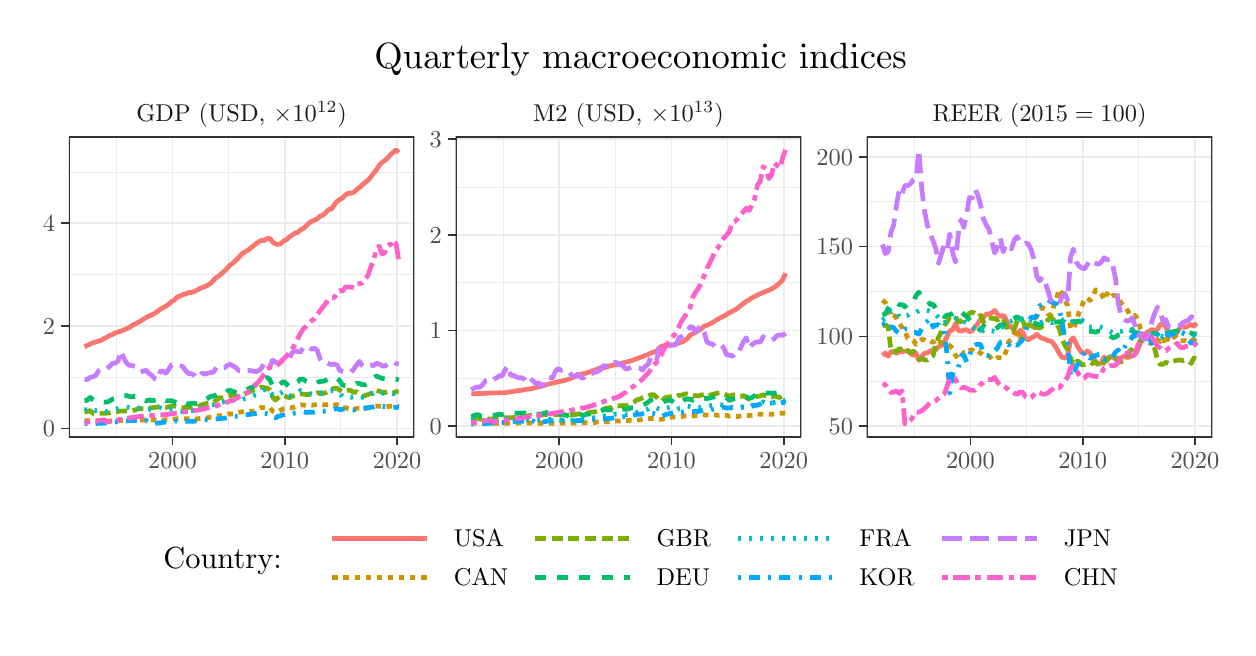
\begin{tikzpicture}[x=1pt,y=1pt]
\definecolor{fillColor}{RGB}{255,255,255}
\path[use as bounding box,fill=fillColor,fill opacity=0.00] (0,0) rectangle (433.62,216.81);
\begin{scope}
\path[clip] (  0.00,  0.00) rectangle (433.62,216.81);
\definecolor{drawColor}{RGB}{255,255,255}
\definecolor{fillColor}{RGB}{255,255,255}

\path[draw=drawColor,line width= 0.6pt,line join=round,line cap=round,fill=fillColor] (  0.00,  0.00) rectangle (433.62,216.81);
\end{scope}
\begin{scope}
\path[clip] ( 14.85, 68.67) rectangle (139.77,177.58);
\definecolor{fillColor}{RGB}{255,255,255}

\path[fill=fillColor] ( 14.85, 68.67) rectangle (139.77,177.58);
\definecolor{drawColor}{gray}{0.92}

\path[draw=drawColor,line width= 0.3pt,line join=round] ( 14.85, 90.55) --
	(139.77, 90.55);

\path[draw=drawColor,line width= 0.3pt,line join=round] ( 14.85,127.59) --
	(139.77,127.59);

\path[draw=drawColor,line width= 0.3pt,line join=round] ( 14.85,164.63) --
	(139.77,164.63);

\path[draw=drawColor,line width= 0.3pt,line join=round] ( 32.03, 68.67) --
	( 32.03,177.58);

\path[draw=drawColor,line width= 0.3pt,line join=round] ( 72.59, 68.67) --
	( 72.59,177.58);

\path[draw=drawColor,line width= 0.3pt,line join=round] (113.15, 68.67) --
	(113.15,177.58);

\path[draw=drawColor,line width= 0.6pt,line join=round] ( 14.85, 72.03) --
	(139.77, 72.03);

\path[draw=drawColor,line width= 0.6pt,line join=round] ( 14.85,109.07) --
	(139.77,109.07);

\path[draw=drawColor,line width= 0.6pt,line join=round] ( 14.85,146.11) --
	(139.77,146.11);

\path[draw=drawColor,line width= 0.6pt,line join=round] ( 52.31, 68.67) --
	( 52.31,177.58);

\path[draw=drawColor,line width= 0.6pt,line join=round] ( 92.87, 68.67) --
	( 92.87,177.58);

\path[draw=drawColor,line width= 0.6pt,line join=round] (133.43, 68.67) --
	(133.43,177.58);
\definecolor{drawColor}{RGB}{248,118,109}

\path[draw=drawColor,line width= 1.7pt,line join=round] ( 20.53,101.49) --
	( 21.55,101.99) --
	( 22.57,102.44) --
	( 23.58,102.96) --
	( 24.58,103.19) --
	( 25.60,103.56) --
	( 26.62,103.89) --
	( 27.63,104.50) --
	( 28.63,104.98) --
	( 29.66,105.58) --
	( 30.68,105.97) --
	( 31.69,106.55) --
	( 32.69,106.86) --
	( 33.71,107.13) --
	( 34.73,107.60) --
	( 35.74,108.02) --
	( 36.75,108.46) --
	( 37.77,109.22) --
	( 38.79,109.68) --
	( 39.81,110.27) --
	( 40.80,110.75) --
	( 41.83,111.47) --
	( 42.85,112.14) --
	( 43.86,112.62) --
	( 44.86,113.08) --
	( 45.88,113.56) --
	( 46.90,114.26) --
	( 47.91,115.06) --
	( 48.91,115.63) --
	( 49.93,116.13) --
	( 50.95,116.86) --
	( 51.96,117.86) --
	( 52.98,118.34) --
	( 54.00,119.48) --
	( 55.02,119.81) --
	( 56.03,120.36) --
	( 57.03,120.52) --
	( 58.05,121.10) --
	( 59.07,121.09) --
	( 60.08,121.39) --
	( 61.08,121.98) --
	( 62.10,122.46) --
	( 63.13,122.92) --
	( 64.14,123.29) --
	( 65.14,123.81) --
	( 66.16,124.41) --
	( 67.18,125.59) --
	( 68.19,126.52) --
	( 69.20,127.22) --
	( 70.22,128.09) --
	( 71.24,128.99) --
	( 72.25,130.01) --
	( 73.25,131.11) --
	( 74.27,131.80) --
	( 75.30,132.88) --
	( 76.31,133.76) --
	( 77.31,135.01) --
	( 78.33,135.69) --
	( 79.35,136.23) --
	( 80.36,137.02) --
	( 81.36,137.81) --
	( 82.38,138.62) --
	( 83.40,139.33) --
	( 84.41,140.00) --
	( 85.42,139.86) --
	( 86.45,140.58) --
	( 87.47,140.71) --
	( 88.48,139.44) --
	( 89.48,138.67) --
	( 90.50,138.48) --
	( 91.52,138.79) --
	( 92.53,139.76) --
	( 93.53,140.19) --
	( 94.55,141.13) --
	( 95.57,141.85) --
	( 96.58,142.59) --
	( 97.58,142.80) --
	( 98.60,143.78) --
	( 99.63,144.22) --
	(100.64,145.16) --
	(101.65,146.20) --
	(102.67,146.81) --
	(103.69,147.30) --
	(104.70,147.77) --
	(105.70,148.74) --
	(106.72,149.06) --
	(107.74,150.04) --
	(108.75,151.12) --
	(109.75,151.22) --
	(110.78,152.74) --
	(111.80,154.08) --
	(112.81,154.67) --
	(113.81,155.29) --
	(114.83,156.38) --
	(115.85,156.96) --
	(116.86,156.99) --
	(117.87,157.33) --
	(118.89,158.32) --
	(119.91,159.10) --
	(120.93,159.96) --
	(121.92,160.88) --
	(122.95,161.65) --
	(123.97,162.83) --
	(124.98,164.25) --
	(125.98,165.38) --
	(127.00,166.99) --
	(128.02,168.10) --
	(129.03,168.78) --
	(130.03,169.71) --
	(131.05,170.83) --
	(132.07,171.77) --
	(133.09,172.63) --
	(134.10,171.75);
\definecolor{drawColor}{RGB}{205,150,0}

\path[draw=drawColor,line width= 1.7pt,dash pattern=on 2pt off 2pt ,line join=round] ( 20.53, 74.83) --
	( 21.55, 74.80) --
	( 22.57, 74.81) --
	( 23.58, 74.70) --
	( 24.58, 74.73) --
	( 25.60, 74.75) --
	( 26.62, 74.70) --
	( 27.63, 74.69) --
	( 28.63, 74.70) --
	( 29.66, 74.66) --
	( 30.68, 74.74) --
	( 31.69, 74.78) --
	( 32.69, 74.75) --
	( 33.71, 74.83) --
	( 34.73, 74.88) --
	( 35.74, 74.90) --
	( 36.75, 74.89) --
	( 37.77, 74.93) --
	( 38.79, 74.95) --
	( 39.81, 75.04) --
	( 40.80, 75.07) --
	( 41.83, 75.04) --
	( 42.85, 75.08) --
	( 43.86, 75.07) --
	( 44.86, 75.06) --
	( 45.88, 75.03) --
	( 46.90, 74.90) --
	( 47.91, 74.90) --
	( 48.91, 75.02) --
	( 49.93, 75.16) --
	( 50.95, 75.22) --
	( 51.96, 75.31) --
	( 52.98, 75.44) --
	( 54.00, 75.47) --
	( 55.02, 75.54) --
	( 56.03, 75.47) --
	( 57.03, 75.52) --
	( 58.05, 75.50) --
	( 59.07, 75.45) --
	( 60.08, 75.36) --
	( 61.08, 75.40) --
	( 62.10, 75.57) --
	( 63.13, 75.60) --
	( 64.14, 75.65) --
	( 65.14, 75.87) --
	( 66.16, 76.14) --
	( 67.18, 76.26) --
	( 68.19, 76.51) --
	( 69.20, 76.59) --
	( 70.22, 76.56) --
	( 71.24, 76.82) --
	( 72.25, 77.22) --
	( 73.25, 77.24) --
	( 74.27, 77.24) --
	( 75.30, 77.57) --
	( 76.31, 77.83) --
	( 77.31, 77.95) --
	( 78.33, 78.18) --
	( 79.35, 78.25) --
	( 80.36, 78.19) --
	( 81.36, 78.15) --
	( 82.38, 78.68) --
	( 83.40, 79.04) --
	( 84.41, 79.60) --
	( 85.42, 79.58) --
	( 86.45, 79.72) --
	( 87.47, 79.56) --
	( 88.48, 78.22) --
	( 89.48, 77.83) --
	( 90.50, 78.17) --
	( 91.52, 78.65) --
	( 92.53, 79.10) --
	( 93.53, 79.34) --
	( 94.55, 79.47) --
	( 95.57, 79.45) --
	( 96.58, 79.81) --
	( 97.58, 80.19) --
	( 98.60, 80.45) --
	( 99.63, 80.47) --
	(100.64, 80.24) --
	(101.65, 80.43) --
	(102.67, 80.37) --
	(103.69, 80.55) --
	(104.70, 80.65) --
	(105.70, 80.65) --
	(106.72, 80.57) --
	(107.74, 80.56) --
	(108.75, 80.56) --
	(109.75, 80.27) --
	(110.78, 80.48) --
	(111.80, 80.60) --
	(112.81, 80.24) --
	(113.81, 79.44) --
	(114.83, 79.51) --
	(115.85, 79.10) --
	(116.86, 78.94) --
	(117.87, 78.78) --
	(118.89, 79.23) --
	(119.91, 79.26) --
	(120.93, 79.20) --
	(121.92, 79.41) --
	(122.95, 79.37) --
	(123.97, 79.95) --
	(124.98, 79.98) --
	(125.98, 80.08) --
	(127.00, 80.00) --
	(128.02, 79.98) --
	(129.03, 79.84) --
	(130.03, 79.91) --
	(131.05, 80.01) --
	(132.07, 80.14) --
	(133.09, 80.22) --
	(134.10, 79.95);
\definecolor{drawColor}{RGB}{124,174,0}

\path[draw=drawColor,line width= 1.7pt,dash pattern=on 4pt off 2pt ,line join=round] ( 20.53, 77.98) --
	( 21.55, 78.12) --
	( 22.57, 78.45) --
	( 23.58, 77.44) --
	( 24.58, 77.22) --
	( 25.60, 77.44) --
	( 26.62, 77.43) --
	( 27.63, 77.45) --
	( 28.63, 77.51) --
	( 29.66, 77.62) --
	( 30.68, 77.86) --
	( 31.69, 78.12) --
	( 32.69, 78.14) --
	( 33.71, 78.27) --
	( 34.73, 78.28) --
	( 35.74, 78.29) --
	( 36.75, 78.29) --
	( 37.77, 78.40) --
	( 38.79, 78.64) --
	( 39.81, 79.07) --
	( 40.80, 79.12) --
	( 41.83, 79.18) --
	( 42.85, 79.33) --
	( 43.86, 79.40) --
	( 44.86, 79.46) --
	( 45.88, 79.58) --
	( 46.90, 79.68) --
	( 47.91, 79.99) --
	( 48.91, 79.84) --
	( 49.93, 79.66) --
	( 50.95, 79.75) --
	( 51.96, 80.04) --
	( 52.98, 80.08) --
	( 54.00, 79.79) --
	( 55.02, 79.57) --
	( 56.03, 79.45) --
	( 57.03, 79.58) --
	( 58.05, 79.55) --
	( 59.07, 79.66) --
	( 60.08, 79.75) --
	( 61.08, 79.74) --
	( 62.10, 80.04) --
	( 63.13, 80.64) --
	( 64.14, 80.88) --
	( 65.14, 81.17) --
	( 66.16, 81.37) --
	( 67.18, 81.47) --
	( 68.19, 82.20) --
	( 69.20, 83.06) --
	( 70.22, 83.07) --
	( 71.24, 83.19) --
	( 72.25, 83.62) --
	( 73.25, 83.89) --
	( 74.27, 83.99) --
	( 75.30, 83.61) --
	( 76.31, 83.66) --
	( 77.31, 83.81) --
	( 78.33, 84.46) --
	( 79.35, 84.90) --
	( 80.36, 85.31) --
	( 81.36, 85.78) --
	( 82.38, 86.16) --
	( 83.40, 86.67) --
	( 84.41, 86.98) --
	( 85.42, 86.73) --
	( 86.45, 86.62) --
	( 87.47, 85.91) --
	( 88.48, 83.38) --
	( 89.48, 82.27) --
	( 90.50, 83.08) --
	( 91.52, 83.86) --
	( 92.53, 83.80) --
	( 93.53, 83.44) --
	( 94.55, 83.09) --
	( 95.57, 83.58) --
	( 96.58, 83.87) --
	( 97.58, 84.33) --
	( 98.60, 84.46) --
	( 99.63, 84.38) --
	(100.64, 84.25) --
	(101.65, 84.30) --
	(102.67, 84.44) --
	(103.69, 84.70) --
	(104.70, 84.96) --
	(105.70, 84.58) --
	(106.72, 84.58) --
	(107.74, 84.95) --
	(108.75, 85.65) --
	(109.75, 86.11) --
	(110.78, 86.50) --
	(111.80, 86.52) --
	(112.81, 85.81) --
	(113.81, 85.28) --
	(114.83, 85.64) --
	(115.85, 85.86) --
	(116.86, 85.63) --
	(117.87, 85.02) --
	(118.89, 85.25) --
	(119.91, 84.21) --
	(120.93, 83.69) --
	(121.92, 83.82) --
	(122.95, 84.25) --
	(123.97, 84.58) --
	(124.98, 84.96) --
	(125.98, 85.71) --
	(127.00, 85.48) --
	(128.02, 85.06) --
	(129.03, 84.94) --
	(130.03, 85.28) --
	(131.05, 85.16) --
	(132.07, 84.75) --
	(133.09, 85.33) --
	(134.10, 85.10);
\definecolor{drawColor}{RGB}{0,190,103}

\path[draw=drawColor,line width= 1.7pt,dash pattern=on 4pt off 4pt ,line join=round] ( 20.53, 82.06) --
	( 21.55, 82.17) --
	( 22.57, 83.20) --
	( 23.58, 82.39) --
	( 24.58, 81.74) --
	( 25.60, 81.97) --
	( 26.62, 81.52) --
	( 27.63, 81.49) --
	( 28.63, 81.53) --
	( 29.66, 81.93) --
	( 30.68, 82.61) --
	( 31.69, 82.87) --
	( 32.69, 83.15) --
	( 33.71, 83.84) --
	( 34.73, 83.79) --
	( 35.74, 83.87) --
	( 36.75, 83.54) --
	( 37.77, 83.39) --
	( 38.79, 83.64) --
	( 39.81, 83.53) --
	( 40.80, 82.62) --
	( 41.83, 82.38) --
	( 42.85, 81.96) --
	( 43.86, 82.31) --
	( 44.86, 82.04) --
	( 45.88, 82.18) --
	( 46.90, 82.42) --
	( 47.91, 83.01) --
	( 48.91, 82.62) --
	( 49.93, 82.03) --
	( 50.95, 82.05) --
	( 51.96, 82.00) --
	( 52.98, 81.62) --
	( 54.00, 81.16) --
	( 55.02, 80.89) --
	( 56.03, 80.53) --
	( 57.03, 81.28) --
	( 58.05, 80.79) --
	( 59.07, 81.02) --
	( 60.08, 81.12) --
	( 61.08, 80.90) --
	( 62.10, 81.34) --
	( 63.13, 82.14) --
	( 64.14, 82.31) --
	( 65.14, 82.95) --
	( 66.16, 83.61) --
	( 67.18, 83.65) --
	( 68.19, 84.34) --
	( 69.20, 85.00) --
	( 70.22, 84.67) --
	( 71.24, 84.83) --
	( 72.25, 85.57) --
	( 73.25, 85.75) --
	( 74.27, 85.29) --
	( 75.30, 84.99) --
	( 76.31, 84.75) --
	( 77.31, 85.00) --
	( 78.33, 85.87) --
	( 79.35, 86.17) --
	( 80.36, 86.61) --
	( 81.36, 86.99) --
	( 82.38, 87.59) --
	( 83.40, 88.04) --
	( 84.41, 89.06) --
	( 85.42, 89.76) --
	( 86.45, 90.53) --
	( 87.47, 89.71) --
	( 88.48, 87.36) --
	( 89.48, 86.62) --
	( 90.50, 87.34) --
	( 91.52, 88.28) --
	( 92.53, 88.98) --
	( 93.53, 88.04) --
	( 94.55, 86.98) --
	( 95.57, 87.49) --
	( 96.58, 88.45) --
	( 97.58, 88.88) --
	( 98.60, 89.85) --
	( 99.63, 89.73) --
	(100.64, 88.98) --
	(101.65, 88.57) --
	(102.67, 88.27) --
	(103.69, 88.04) --
	(104.70, 88.65) --
	(105.70, 88.96) --
	(106.72, 89.02) --
	(107.74, 89.43) --
	(108.75, 90.00) --
	(109.75, 90.45) --
	(110.78, 90.55) --
	(111.80, 90.05) --
	(112.81, 89.20) --
	(113.81, 87.60) --
	(114.83, 87.51) --
	(115.85, 87.74) --
	(116.86, 87.53) --
	(117.87, 87.84) --
	(118.89, 88.36) --
	(119.91, 88.25) --
	(120.93, 87.76) --
	(121.92, 87.76) --
	(122.95, 88.47) --
	(123.97, 89.84) --
	(124.98, 90.06) --
	(125.98, 90.94) --
	(127.00, 90.48) --
	(128.02, 90.09) --
	(129.03, 89.92) --
	(130.03, 89.99) --
	(131.05, 89.87) --
	(132.07, 89.78) --
	(133.09, 89.84) --
	(134.10, 89.49);
\definecolor{drawColor}{RGB}{0,191,196}

\path[draw=drawColor,line width= 1.7pt,dash pattern=on 1pt off 3pt ,line join=round] ( 20.53, 78.75) --
	( 21.55, 78.79) --
	( 22.57, 79.46) --
	( 23.58, 78.84) --
	( 24.58, 78.43) --
	( 25.60, 78.52) --
	( 26.62, 78.21) --
	( 27.63, 78.17) --
	( 28.63, 78.13) --
	( 29.66, 78.45) --
	( 30.68, 78.87) --
	( 31.69, 79.00) --
	( 32.69, 79.22) --
	( 33.71, 79.61) --
	( 34.73, 79.57) --
	( 35.74, 79.65) --
	( 36.75, 79.59) --
	( 37.77, 79.42) --
	( 38.79, 79.59) --
	( 39.81, 79.48) --
	( 40.80, 78.97) --
	( 41.83, 78.84) --
	( 42.85, 78.57) --
	( 43.86, 78.85) --
	( 44.86, 78.69) --
	( 45.88, 78.86) --
	( 46.90, 79.02) --
	( 47.91, 79.47) --
	( 48.91, 79.19) --
	( 49.93, 78.83) --
	( 50.95, 78.86) --
	( 51.96, 78.89) --
	( 52.98, 78.66) --
	( 54.00, 78.39) --
	( 55.02, 78.26) --
	( 56.03, 78.10) --
	( 57.03, 78.54) --
	( 58.05, 78.24) --
	( 59.07, 78.41) --
	( 60.08, 78.48) --
	( 61.08, 78.41) --
	( 62.10, 78.77) --
	( 63.13, 79.31) --
	( 64.14, 79.48) --
	( 65.14, 80.05) --
	( 66.16, 80.55) --
	( 67.18, 80.57) --
	( 68.19, 81.17) --
	( 69.20, 81.75) --
	( 70.22, 81.49) --
	( 71.24, 81.68) --
	( 72.25, 82.40) --
	( 73.25, 82.59) --
	( 74.27, 82.25) --
	( 75.30, 82.02) --
	( 76.31, 81.91) --
	( 77.31, 82.14) --
	( 78.33, 82.75) --
	( 79.35, 82.98) --
	( 80.36, 83.29) --
	( 81.36, 83.61) --
	( 82.38, 84.11) --
	( 83.40, 84.48) --
	( 84.41, 85.27) --
	( 85.42, 85.89) --
	( 86.45, 86.49) --
	( 87.47, 85.89) --
	( 88.48, 84.06) --
	( 89.48, 83.74) --
	( 90.50, 84.20) --
	( 91.52, 84.80) --
	( 92.53, 85.37) --
	( 93.53, 84.62) --
	( 94.55, 83.70) --
	( 95.57, 84.03) --
	( 96.58, 84.74) --
	( 97.58, 84.98) --
	( 98.60, 85.70) --
	( 99.63, 85.51) --
	(100.64, 84.96) --
	(101.65, 84.68) --
	(102.67, 84.42) --
	(103.69, 84.17) --
	(104.70, 84.62) --
	(105.70, 84.87) --
	(106.72, 84.85) --
	(107.74, 85.05) --
	(108.75, 85.46) --
	(109.75, 85.62) --
	(110.78, 85.64) --
	(111.80, 85.24) --
	(112.81, 84.56) --
	(113.81, 83.44) --
	(114.83, 83.25) --
	(115.85, 83.41) --
	(116.86, 83.24) --
	(117.87, 83.43) --
	(118.89, 83.66) --
	(119.91, 83.56) --
	(120.93, 83.22) --
	(121.92, 83.23) --
	(122.95, 83.69) --
	(123.97, 84.58) --
	(124.98, 84.73) --
	(125.98, 85.39) --
	(127.00, 85.01) --
	(128.02, 84.78) --
	(129.03, 84.65) --
	(130.03, 84.70) --
	(131.05, 84.64) --
	(132.07, 84.56) --
	(133.09, 84.56) --
	(134.10, 83.96);
\definecolor{drawColor}{RGB}{0,169,255}

\path[draw=drawColor,line width= 1.7pt,dash pattern=on 1pt off 3pt on 4pt off 3pt ,line join=round] ( 20.53, 73.63) --
	( 21.55, 73.66) --
	( 22.57, 73.68) --
	( 23.58, 73.73) --
	( 24.58, 73.77) --
	( 25.60, 73.84) --
	( 26.62, 73.87) --
	( 27.63, 73.93) --
	( 28.63, 74.05) --
	( 29.66, 74.13) --
	( 30.68, 74.22) --
	( 31.69, 74.34) --
	( 32.69, 74.47) --
	( 33.71, 74.66) --
	( 34.73, 74.76) --
	( 35.74, 74.77) --
	( 36.75, 74.84) --
	( 37.77, 74.90) --
	( 38.79, 74.87) --
	( 39.81, 74.87) --
	( 40.80, 74.79) --
	( 41.83, 74.82) --
	( 42.85, 74.88) --
	( 43.86, 74.33) --
	( 44.86, 73.62) --
	( 45.88, 73.79) --
	( 46.90, 73.90) --
	( 47.91, 73.99) --
	( 48.91, 74.20) --
	( 49.93, 74.27) --
	( 50.95, 74.38) --
	( 51.96, 74.50) --
	( 52.98, 74.65) --
	( 54.00, 74.70) --
	( 55.02, 74.78) --
	( 56.03, 74.67) --
	( 57.03, 74.54) --
	( 58.05, 74.54) --
	( 59.07, 74.61) --
	( 60.08, 74.60) --
	( 61.08, 74.71) --
	( 62.10, 74.89) --
	( 63.13, 75.09) --
	( 64.14, 75.10) --
	( 65.14, 75.19) --
	( 66.16, 75.20) --
	( 67.18, 75.34) --
	( 68.19, 75.43) --
	( 69.20, 75.55) --
	( 70.22, 75.64) --
	( 71.24, 75.70) --
	( 72.25, 75.95) --
	( 73.25, 76.26) --
	( 74.27, 76.39) --
	( 75.30, 76.39) --
	( 76.31, 76.42) --
	( 77.31, 76.71) --
	( 78.33, 76.87) --
	( 79.35, 76.96) --
	( 80.36, 77.11) --
	( 81.36, 77.23) --
	( 82.38, 77.41) --
	( 83.40, 77.51) --
	( 84.41, 77.71) --
	( 85.42, 77.52) --
	( 86.45, 77.31) --
	( 87.47, 77.13) --
	( 88.48, 75.94) --
	( 89.48, 75.82) --
	( 90.50, 76.33) --
	( 91.52, 76.63) --
	( 92.53, 76.94) --
	( 93.53, 77.22) --
	( 94.55, 77.26) --
	( 95.57, 77.26) --
	( 96.58, 77.58) --
	( 97.58, 77.68) --
	( 98.60, 77.91) --
	( 99.63, 77.98) --
	(100.64, 77.78) --
	(101.65, 77.89) --
	(102.67, 77.79) --
	(103.69, 77.92) --
	(104.70, 78.22) --
	(105.70, 78.32) --
	(106.72, 78.19) --
	(107.74, 78.34) --
	(108.75, 78.69) --
	(109.75, 78.73) --
	(110.78, 79.03) --
	(111.80, 79.08) --
	(112.81, 78.79) --
	(113.81, 78.91) --
	(114.83, 78.99) --
	(115.85, 78.62) --
	(116.86, 78.77) --
	(117.87, 78.65) --
	(118.89, 78.96) --
	(119.91, 79.22) --
	(120.93, 79.10) --
	(121.92, 79.26) --
	(122.95, 79.47) --
	(123.97, 79.68) --
	(124.98, 79.78) --
	(125.98, 80.10) --
	(127.00, 80.15) --
	(128.02, 79.95) --
	(129.03, 79.88) --
	(130.03, 79.82) --
	(131.05, 79.65) --
	(132.07, 79.50) --
	(133.09, 79.67) --
	(134.10, 79.43);
\definecolor{drawColor}{RGB}{199,124,255}

\path[draw=drawColor,line width= 1.7pt,dash pattern=on 7pt off 3pt ,line join=round] ( 20.53, 89.75) --
	( 21.55, 89.66) --
	( 22.57, 90.47) --
	( 23.58, 90.65) --
	( 24.58, 91.13) --
	( 25.60, 92.82) --
	( 26.62, 93.62) --
	( 27.63, 93.23) --
	( 28.63, 93.57) --
	( 29.66, 94.45) --
	( 30.68, 95.55) --
	( 31.69, 95.56) --
	( 32.69, 96.39) --
	( 33.71,100.02) --
	( 34.73, 97.40) --
	( 35.74, 95.64) --
	( 36.75, 94.79) --
	( 37.77, 94.70) --
	( 38.79, 94.38) --
	( 39.81, 93.81) --
	( 40.80, 92.37) --
	( 41.83, 92.73) --
	( 42.85, 93.01) --
	( 43.86, 91.81) --
	( 44.86, 91.17) --
	( 45.88, 89.98) --
	( 46.90, 89.42) --
	( 47.91, 92.61) --
	( 48.91, 92.72) --
	( 49.93, 91.98) --
	( 50.95, 93.30) --
	( 51.96, 95.06) --
	( 52.98, 94.82) --
	( 54.00, 94.88) --
	( 55.02, 94.64) --
	( 56.03, 94.33) --
	( 57.03, 92.90) --
	( 58.05, 91.89) --
	( 59.07, 91.80) --
	( 60.08, 91.32) --
	( 61.08, 90.11) --
	( 62.10, 90.87) --
	( 63.13, 92.04) --
	( 64.14, 91.54) --
	( 65.14, 91.98) --
	( 66.16, 92.19) --
	( 67.18, 92.38) --
	( 68.19, 94.07) --
	( 69.20, 94.52) --
	( 70.22, 93.95) --
	( 71.24, 94.01) --
	( 72.25, 94.87) --
	( 73.25, 95.14) --
	( 74.27, 94.55) --
	( 75.30, 93.92) --
	( 76.31, 92.81) --
	( 77.31, 92.86) --
	( 78.33, 93.30) --
	( 79.35, 92.90) --
	( 80.36, 92.92) --
	( 81.36, 92.73) --
	( 82.38, 92.51) --
	( 83.40, 92.83) --
	( 84.41, 93.70) --
	( 85.42, 95.33) --
	( 86.45, 95.34) --
	( 87.47, 94.24) --
	( 88.48, 96.63) --
	( 89.48, 96.07) --
	( 90.50, 95.43) --
	( 91.52, 96.19) --
	( 92.53, 97.38) --
	( 93.53, 97.35) --
	( 94.55, 97.18) --
	( 95.57, 99.34) --
	( 96.58,100.09) --
	( 97.58, 99.73) --
	( 98.60, 99.54) --
	( 99.63,101.53) --
	(100.64,101.63) --
	(101.65,101.27) --
	(102.67,100.61) --
	(103.69,101.00) --
	(104.70,100.10) --
	(105.70, 97.02) --
	(106.72, 95.58) --
	(107.74, 95.76) --
	(108.75, 95.38) --
	(109.75, 95.11) --
	(110.78, 95.26) --
	(111.80, 94.87) --
	(112.81, 92.93) --
	(113.81, 92.60) --
	(114.83, 92.31) --
	(115.85, 92.25) --
	(116.86, 92.30) --
	(117.87, 93.54) --
	(118.89, 94.95) --
	(119.91, 96.24) --
	(120.93, 94.70) --
	(121.92, 94.06) --
	(122.95, 94.67) --
	(123.97, 94.94) --
	(124.98, 94.66) --
	(125.98, 95.51) --
	(127.00, 95.32) --
	(128.02, 94.68) --
	(129.03, 94.47) --
	(130.03, 95.25) --
	(131.05, 95.46) --
	(132.07, 96.13) --
	(133.09, 95.44) --
	(134.10, 95.26);
\definecolor{drawColor}{RGB}{255,97,204}

\path[draw=drawColor,line width= 1.7pt,dash pattern=on 2pt off 2pt on 6pt off 2pt ,line join=round] ( 20.53, 74.09) --
	( 21.55, 74.25) --
	( 22.57, 74.40) --
	( 23.58, 74.44) --
	( 24.58, 74.56) --
	( 25.60, 74.78) --
	( 26.62, 74.96) --
	( 27.63, 75.16) --
	( 28.63, 74.34) --
	( 29.66, 74.53) --
	( 30.68, 74.74) --
	( 31.69, 74.92) --
	( 32.69, 75.10) --
	( 33.71, 75.34) --
	( 34.73, 75.55) --
	( 35.74, 75.67) --
	( 36.75, 75.79) --
	( 37.77, 75.94) --
	( 38.79, 76.09) --
	( 39.81, 76.25) --
	( 40.80, 76.32) --
	( 41.83, 76.43) --
	( 42.85, 76.52) --
	( 43.86, 76.64) --
	( 44.86, 76.65) --
	( 45.88, 76.70) --
	( 46.90, 76.82) --
	( 47.91, 76.99) --
	( 48.91, 76.95) --
	( 49.93, 77.00) --
	( 50.95, 77.11) --
	( 51.96, 77.31) --
	( 52.98, 77.41) --
	( 54.00, 77.56) --
	( 55.02, 77.70) --
	( 56.03, 77.87) --
	( 57.03, 78.06) --
	( 58.05, 78.17) --
	( 59.07, 78.28) --
	( 60.08, 78.41) --
	( 61.08, 78.57) --
	( 62.10, 78.73) --
	( 63.13, 78.92) --
	( 64.14, 79.11) --
	( 65.14, 79.40) --
	( 66.16, 79.49) --
	( 67.18, 79.81) --
	( 68.19, 80.13) --
	( 69.20, 80.53) --
	( 70.22, 80.89) --
	( 71.24, 81.27) --
	( 72.25, 81.59) --
	( 73.25, 81.95) --
	( 74.27, 82.25) --
	( 75.30, 82.83) --
	( 76.31, 83.37) --
	( 77.31, 83.89) --
	( 78.33, 84.40) --
	( 79.35, 84.92) --
	( 80.36, 85.79) --
	( 81.36, 86.99) --
	( 82.38, 87.86) --
	( 83.40, 88.86) --
	( 84.41, 90.04) --
	( 85.42, 91.75) --
	( 86.45, 93.22) --
	( 87.47, 94.06) --
	( 88.48, 94.10) --
	( 89.48, 94.10) --
	( 90.50, 95.02) --
	( 91.52, 96.04) --
	( 92.53, 97.15) --
	( 93.53, 98.20) --
	( 94.55, 99.29) --
	( 95.57,100.58) --
	( 96.58,102.51) --
	( 97.58,104.44) --
	( 98.60,106.33) --
	( 99.63,107.97) --
	(100.64,108.92) --
	(101.65,110.04) --
	(102.67,110.97) --
	(103.69,111.64) --
	(104.70,113.28) --
	(105.70,114.55) --
	(106.72,115.87) --
	(107.74,117.28) --
	(108.75,118.70) --
	(109.75,119.25) --
	(110.78,119.24) --
	(111.80,120.93) --
	(112.81,121.85) --
	(113.81,121.62) --
	(114.83,123.08) --
	(115.85,123.06) --
	(116.86,123.10) --
	(117.87,122.77) --
	(118.89,124.15) --
	(119.91,124.33) --
	(120.93,124.52) --
	(121.92,125.91) --
	(122.95,127.29) --
	(123.97,130.30) --
	(124.98,132.43) --
	(125.98,136.93) --
	(127.00,137.89) --
	(128.02,134.96) --
	(129.03,135.48) --
	(130.03,138.03) --
	(131.05,138.68) --
	(132.07,137.63) --
	(133.09,138.95) --
	(134.10,132.51);
\definecolor{drawColor}{gray}{0.20}

\path[draw=drawColor,line width= 1.1pt,line join=round,line cap=round] ( 14.85, 68.67) rectangle (139.77,177.58);
\end{scope}
\begin{scope}
\path[clip] (154.62, 68.67) rectangle (279.55,177.58);
\definecolor{fillColor}{RGB}{255,255,255}

\path[fill=fillColor] (154.62, 68.67) rectangle (279.55,177.58);
\definecolor{drawColor}{gray}{0.92}

\path[draw=drawColor,line width= 0.3pt,line join=round] (154.62, 90.09) --
	(279.55, 90.09);

\path[draw=drawColor,line width= 0.3pt,line join=round] (154.62,124.65) --
	(279.55,124.65);

\path[draw=drawColor,line width= 0.3pt,line join=round] (154.62,159.20) --
	(279.55,159.20);

\path[draw=drawColor,line width= 0.3pt,line join=round] (171.80, 68.67) --
	(171.80,177.58);

\path[draw=drawColor,line width= 0.3pt,line join=round] (212.37, 68.67) --
	(212.37,177.58);

\path[draw=drawColor,line width= 0.3pt,line join=round] (252.93, 68.67) --
	(252.93,177.58);

\path[draw=drawColor,line width= 0.6pt,line join=round] (154.62, 72.82) --
	(279.55, 72.82);

\path[draw=drawColor,line width= 0.6pt,line join=round] (154.62,107.37) --
	(279.55,107.37);

\path[draw=drawColor,line width= 0.6pt,line join=round] (154.62,141.92) --
	(279.55,141.92);

\path[draw=drawColor,line width= 0.6pt,line join=round] (154.62,176.48) --
	(279.55,176.48);

\path[draw=drawColor,line width= 0.6pt,line join=round] (192.08, 68.67) --
	(192.08,177.58);

\path[draw=drawColor,line width= 0.6pt,line join=round] (232.65, 68.67) --
	(232.65,177.58);

\path[draw=drawColor,line width= 0.6pt,line join=round] (273.20, 68.67) --
	(273.20,177.58);
\definecolor{drawColor}{RGB}{248,118,109}

\path[draw=drawColor,line width= 1.7pt,line join=round] (160.30, 84.58) --
	(161.32, 84.54) --
	(162.34, 84.60) --
	(163.36, 84.65) --
	(164.35, 84.60) --
	(165.38, 84.71) --
	(166.40, 84.74) --
	(167.41, 84.82) --
	(168.41, 84.84) --
	(169.43, 84.84) --
	(170.45, 84.86) --
	(171.46, 84.86) --
	(172.46, 84.88) --
	(173.48, 85.08) --
	(174.50, 85.26) --
	(175.51, 85.36) --
	(176.53, 85.56) --
	(177.55, 85.68) --
	(178.57, 85.79) --
	(179.58, 86.01) --
	(180.58, 86.16) --
	(181.60, 86.31) --
	(182.62, 86.54) --
	(183.63, 86.75) --
	(184.63, 87.03) --
	(185.65, 87.27) --
	(186.68, 87.56) --
	(187.69, 87.93) --
	(188.69, 88.13) --
	(189.71, 88.39) --
	(190.73, 88.60) --
	(191.74, 88.84) --
	(192.75, 89.09) --
	(193.77, 89.30) --
	(194.79, 89.59) --
	(195.80, 89.83) --
	(196.80, 90.34) --
	(197.82, 90.69) --
	(198.85, 91.30) --
	(199.86, 91.59) --
	(200.86, 91.80) --
	(201.88, 91.98) --
	(202.90, 92.36) --
	(203.91, 92.76) --
	(204.91, 93.07) --
	(205.93, 93.53) --
	(206.95, 93.80) --
	(207.96, 93.78) --
	(208.97, 94.07) --
	(210.00, 94.48) --
	(211.02, 94.74) --
	(212.03, 94.99) --
	(213.03, 95.08) --
	(214.05, 95.30) --
	(215.07, 95.64) --
	(216.08, 95.90) --
	(217.08, 96.18) --
	(218.10, 96.47) --
	(219.12, 96.81) --
	(220.13, 97.25) --
	(221.13, 97.55) --
	(222.15, 97.97) --
	(223.18, 98.40) --
	(224.19, 98.63) --
	(225.20, 99.27) --
	(226.22, 99.52) --
	(227.24, 99.97) --
	(228.25,101.12) --
	(229.25,101.74) --
	(230.27,101.98) --
	(231.29,101.99) --
	(232.30,102.17) --
	(233.30,102.20) --
	(234.33,102.56) --
	(235.35,102.88) --
	(236.36,103.23) --
	(237.36,103.72) --
	(238.38,104.44) --
	(239.40,105.74) --
	(240.41,106.20) --
	(241.42,106.78) --
	(242.44,107.37) --
	(243.46,108.06) --
	(244.48,108.96) --
	(245.47,109.27) --
	(246.50,109.74) --
	(247.52,110.28) --
	(248.53,110.93) --
	(249.53,111.52) --
	(250.55,112.14) --
	(251.57,112.56) --
	(252.58,113.18) --
	(253.58,113.86) --
	(254.60,114.30) --
	(255.62,114.85) --
	(256.64,115.47) --
	(257.65,116.39) --
	(258.67,117.16) --
	(259.69,117.87) --
	(260.70,118.46) --
	(261.70,119.19) --
	(262.72,119.67) --
	(263.74,120.23) --
	(264.75,120.68) --
	(265.75,121.07) --
	(266.77,121.55) --
	(267.80,121.93) --
	(268.81,122.43) --
	(269.81,122.96) --
	(270.83,123.80) --
	(271.85,124.66) --
	(272.86,125.75) --
	(273.87,128.06);
\definecolor{drawColor}{RGB}{205,150,0}

\path[draw=drawColor,line width= 1.7pt,dash pattern=on 2pt off 2pt ,line join=round] (160.30, 73.95) --
	(161.32, 73.95) --
	(162.34, 73.95) --
	(163.36, 73.91) --
	(164.35, 73.93) --
	(165.38, 73.92) --
	(166.40, 73.89) --
	(167.41, 73.88) --
	(168.41, 73.85) --
	(169.43, 73.85) --
	(170.45, 73.89) --
	(171.46, 73.87) --
	(172.46, 73.87) --
	(173.48, 73.90) --
	(174.50, 73.94) --
	(175.51, 73.93) --
	(176.53, 73.95) --
	(177.55, 73.95) --
	(178.57, 73.95) --
	(179.58, 73.95) --
	(180.58, 73.94) --
	(181.60, 73.94) --
	(182.62, 73.93) --
	(183.63, 73.89) --
	(184.63, 73.89) --
	(185.65, 73.86) --
	(186.68, 73.83) --
	(187.69, 73.82) --
	(188.69, 73.85) --
	(189.71, 73.89) --
	(190.73, 73.90) --
	(191.74, 73.93) --
	(192.75, 73.97) --
	(193.77, 73.97) --
	(194.79, 73.98) --
	(195.80, 73.97) --
	(196.80, 73.96) --
	(197.82, 73.99) --
	(198.85, 73.97) --
	(199.86, 73.99) --
	(200.86, 74.00) --
	(201.88, 74.05) --
	(202.90, 74.04) --
	(203.91, 74.07) --
	(204.91, 74.15) --
	(205.93, 74.30) --
	(206.95, 74.31) --
	(207.96, 74.39) --
	(208.97, 74.40) --
	(210.00, 74.39) --
	(211.02, 74.49) --
	(212.03, 74.62) --
	(213.03, 74.66) --
	(214.05, 74.64) --
	(215.07, 74.75) --
	(216.08, 74.81) --
	(217.08, 74.87) --
	(218.10, 74.98) --
	(219.12, 75.03) --
	(220.13, 75.01) --
	(221.13, 75.01) --
	(222.15, 75.26) --
	(223.18, 75.42) --
	(224.19, 75.51) --
	(225.20, 75.58) --
	(226.22, 75.60) --
	(227.24, 75.57) --
	(228.25, 75.31) --
	(229.25, 75.34) --
	(230.27, 75.69) --
	(231.29, 75.89) --
	(232.30, 76.00) --
	(233.30, 76.15) --
	(234.33, 76.15) --
	(235.35, 76.22) --
	(236.36, 76.33) --
	(237.36, 76.49) --
	(238.38, 76.52) --
	(239.40, 76.51) --
	(240.41, 76.50) --
	(241.42, 76.65) --
	(242.44, 76.61) --
	(243.46, 76.84) --
	(244.48, 76.87) --
	(245.47, 76.83) --
	(246.50, 76.83) --
	(247.52, 76.89) --
	(248.53, 76.85) --
	(249.53, 76.72) --
	(250.55, 76.86) --
	(251.57, 76.86) --
	(252.58, 76.71) --
	(253.58, 76.42) --
	(254.60, 76.53) --
	(255.62, 76.37) --
	(256.64, 76.29) --
	(257.65, 76.49) --
	(258.67, 76.65) --
	(259.69, 76.70) --
	(260.70, 76.69) --
	(261.70, 76.75) --
	(262.72, 76.85) --
	(263.74, 77.19) --
	(264.75, 77.10) --
	(265.75, 77.11) --
	(266.77, 77.05) --
	(267.80, 77.14) --
	(268.81, 77.11) --
	(269.81, 77.22) --
	(270.83, 77.29) --
	(271.85, 77.40) --
	(272.86, 77.54) --
	(273.87, 77.45);
\definecolor{drawColor}{RGB}{124,174,0}

\path[draw=drawColor,line width= 1.7pt,dash pattern=on 4pt off 2pt ,line join=round] (160.30, 75.61) --
	(161.32, 75.84) --
	(162.34, 75.86) --
	(163.36, 75.40) --
	(164.35, 75.27) --
	(165.38, 75.37) --
	(166.40, 75.44) --
	(167.41, 75.44) --
	(168.41, 75.48) --
	(169.43, 75.54) --
	(170.45, 75.64) --
	(171.46, 75.66) --
	(172.46, 75.82) --
	(173.48, 75.85) --
	(174.50, 75.88) --
	(175.51, 75.91) --
	(176.53, 75.96) --
	(177.55, 76.07) --
	(178.57, 76.20) --
	(179.58, 76.49) --
	(180.58, 76.49) --
	(181.60, 76.75) --
	(182.62, 76.47) --
	(183.63, 76.79) --
	(184.63, 76.84) --
	(185.65, 76.86) --
	(186.68, 77.01) --
	(187.69, 77.05) --
	(188.69, 76.90) --
	(189.71, 76.91) --
	(190.73, 76.96) --
	(191.74, 77.03) --
	(192.75, 77.00) --
	(193.77, 76.95) --
	(194.79, 76.80) --
	(195.80, 77.00) --
	(196.80, 77.05) --
	(197.82, 76.95) --
	(198.85, 77.27) --
	(199.86, 77.26) --
	(200.86, 77.20) --
	(201.88, 77.45) --
	(202.90, 77.75) --
	(203.91, 77.94) --
	(204.91, 77.96) --
	(205.93, 78.32) --
	(206.95, 78.23) --
	(207.96, 78.86) --
	(208.97, 79.26) --
	(210.00, 79.44) --
	(211.02, 79.47) --
	(212.03, 80.14) --
	(213.03, 80.23) --
	(214.05, 80.13) --
	(215.07, 80.26) --
	(216.08, 80.22) --
	(217.08, 80.42) --
	(218.10, 81.08) --
	(219.12, 81.55) --
	(220.13, 82.31) --
	(221.13, 82.52) --
	(222.15, 83.10) --
	(223.18, 83.55) --
	(224.19, 83.63) --
	(225.20, 84.17) --
	(226.22, 84.18) --
	(227.24, 83.31) --
	(228.25, 82.25) --
	(229.25, 81.90) --
	(230.27, 83.08) --
	(231.29, 83.30) --
	(232.30, 83.47) --
	(233.30, 83.76) --
	(234.33, 83.49) --
	(235.35, 84.02) --
	(236.36, 84.02) --
	(237.36, 84.45) --
	(238.38, 84.49) --
	(239.40, 84.21) --
	(240.41, 83.78) --
	(241.42, 83.88) --
	(242.44, 83.72) --
	(243.46, 84.08) --
	(244.48, 84.22) --
	(245.47, 83.63) --
	(246.50, 83.99) --
	(247.52, 84.28) --
	(248.53, 84.58) --
	(249.53, 84.78) --
	(250.55, 84.88) --
	(251.57, 84.50) --
	(252.58, 84.05) --
	(253.58, 83.62) --
	(254.60, 84.06) --
	(255.62, 84.04) --
	(256.64, 83.86) --
	(257.65, 83.56) --
	(258.67, 83.83) --
	(259.69, 83.15) --
	(260.70, 82.64) --
	(261.70, 82.60) --
	(262.72, 83.06) --
	(263.74, 83.58) --
	(264.75, 83.72) --
	(265.75, 84.16) --
	(266.77, 83.70) --
	(267.80, 83.59) --
	(268.81, 83.38) --
	(269.81, 83.80) --
	(270.83, 83.40) --
	(271.85, 83.17) --
	(272.86, 83.88) --
	(273.87, 83.95);
\definecolor{drawColor}{RGB}{0,190,103}

\path[draw=drawColor,line width= 1.7pt,dash pattern=on 4pt off 4pt ,line join=round] (160.30, 76.38) --
	(161.32, 76.64) --
	(162.34, 77.03) --
	(163.36, 76.62) --
	(164.35, 76.50) --
	(165.38, 76.58) --
	(166.40, 76.62) --
	(167.41, 76.61) --
	(168.41, 76.73) --
	(169.43, 76.92) --
	(170.45, 77.11) --
	(171.46, 76.97) --
	(172.46, 77.28) --
	(173.48, 77.38) --
	(174.50, 77.31) --
	(175.51, 77.46) --
	(176.53, 77.49) --
	(177.55, 77.44) --
	(178.57, 77.60) --
	(179.58, 77.61) --
	(180.58, 77.21) --
	(181.60, 77.18) --
	(182.62, 77.09) --
	(183.63, 77.15) --
	(184.63, 77.08) --
	(185.65, 77.22) --
	(186.68, 77.52) --
	(187.69, 77.79) --
	(188.69, 77.53) --
	(189.71, 77.40) --
	(190.73, 77.48) --
	(191.74, 77.33) --
	(192.75, 77.15) --
	(193.77, 77.03) --
	(194.79, 76.65) --
	(195.80, 76.81) --
	(196.80, 76.92) --
	(197.82, 76.72) --
	(198.85, 77.05) --
	(199.86, 76.95) --
	(200.86, 76.68) --
	(201.88, 77.08) --
	(202.90, 77.21) --
	(203.91, 77.50) --
	(204.91, 77.87) --
	(205.93, 78.36) --
	(206.95, 78.17) --
	(207.96, 78.67) --
	(208.97, 78.75) --
	(210.00, 78.66) --
	(211.02, 78.77) --
	(212.03, 79.34) --
	(213.03, 79.32) --
	(214.05, 78.91) --
	(215.07, 79.03) --
	(216.08, 78.87) --
	(217.08, 79.05) --
	(218.10, 79.48) --
	(219.12, 79.53) --
	(220.13, 79.92) --
	(221.13, 80.03) --
	(222.15, 80.30) --
	(223.18, 80.81) --
	(224.19, 81.50) --
	(225.20, 82.24) --
	(226.22, 82.42) --
	(227.24, 81.86) --
	(228.25, 81.56) --
	(229.25, 81.32) --
	(230.27, 81.90) --
	(231.29, 82.18) --
	(232.30, 82.15) --
	(233.30, 81.58) --
	(234.33, 80.82) --
	(235.35, 81.45) --
	(236.36, 81.66) --
	(237.36, 82.34) --
	(238.38, 82.72) --
	(239.40, 82.48) --
	(240.41, 82.19) --
	(241.42, 82.42) --
	(242.44, 82.17) --
	(243.46, 82.59) --
	(244.48, 82.91) --
	(245.47, 82.77) --
	(246.50, 83.03) --
	(247.52, 83.28) --
	(248.53, 83.66) --
	(249.53, 83.88) --
	(250.55, 83.83) --
	(251.57, 83.39) --
	(252.58, 83.05) --
	(253.58, 82.06) --
	(254.60, 82.57) --
	(255.62, 82.77) --
	(256.64, 82.65) --
	(257.65, 83.01) --
	(258.67, 83.25) --
	(259.69, 83.38) --
	(260.70, 82.87) --
	(261.70, 83.19) --
	(262.72, 83.84) --
	(263.74, 84.57) --
	(264.75, 84.64) --
	(265.75, 85.21) --
	(266.77, 84.71) --
	(267.80, 84.83) --
	(268.81, 84.72) --
	(269.81, 84.76) --
	(270.83, 84.91) --
	(271.85, 84.73) --
	(272.86, 84.99) --
	(273.87, 85.31);
\definecolor{drawColor}{RGB}{0,191,196}

\path[draw=drawColor,line width= 1.7pt,dash pattern=on 1pt off 3pt ,line join=round] (160.30, 75.03) --
	(161.32, 75.13) --
	(162.34, 75.29) --
	(163.36, 75.04) --
	(164.35, 74.92) --
	(165.38, 74.91) --
	(166.40, 74.89) --
	(167.41, 74.80) --
	(168.41, 74.85) --
	(169.43, 74.93) --
	(170.45, 75.05) --
	(171.46, 75.05) --
	(172.46, 75.29) --
	(173.48, 75.39) --
	(174.50, 75.36) --
	(175.51, 75.45) --
	(176.53, 75.35) --
	(177.55, 75.29) --
	(178.57, 75.34) --
	(179.58, 75.32) --
	(180.58, 75.11) --
	(181.60, 75.11) --
	(182.62, 75.10) --
	(183.63, 75.16) --
	(184.63, 75.16) --
	(185.65, 75.26) --
	(186.68, 75.38) --
	(187.69, 75.41) --
	(188.69, 75.30) --
	(189.71, 75.20) --
	(190.73, 75.24) --
	(191.74, 75.18) --
	(192.75, 75.08) --
	(193.77, 75.09) --
	(194.79, 74.95) --
	(195.80, 75.05) --
	(196.80, 75.10) --
	(197.82, 75.01) --
	(198.85, 75.18) --
	(199.86, 75.18) --
	(200.86, 75.21) --
	(201.88, 75.46) --
	(202.90, 75.61) --
	(203.91, 75.74) --
	(204.91, 75.94) --
	(205.93, 76.20) --
	(206.95, 76.12) --
	(207.96, 76.50) --
	(208.97, 76.53) --
	(210.00, 76.55) --
	(211.02, 76.64) --
	(212.03, 77.10) --
	(213.03, 77.12) --
	(214.05, 76.88) --
	(215.07, 76.97) --
	(216.08, 76.92) --
	(217.08, 77.05) --
	(218.10, 77.39) --
	(219.12, 77.49) --
	(220.13, 77.75) --
	(221.13, 77.98) --
	(222.15, 78.20) --
	(223.18, 78.53) --
	(224.19, 78.99) --
	(225.20, 79.61) --
	(226.22, 79.69) --
	(227.24, 79.29) --
	(228.25, 79.02) --
	(229.25, 78.70) --
	(230.27, 79.12) --
	(231.29, 79.44) --
	(232.30, 79.49) --
	(233.30, 79.12) --
	(234.33, 78.62) --
	(235.35, 79.15) --
	(236.36, 79.34) --
	(237.36, 79.82) --
	(238.38, 80.09) --
	(239.40, 79.87) --
	(240.41, 79.57) --
	(241.42, 79.80) --
	(242.44, 79.45) --
	(243.46, 79.68) --
	(244.48, 79.96) --
	(245.47, 79.95) --
	(246.50, 80.18) --
	(247.52, 80.33) --
	(248.53, 80.50) --
	(249.53, 80.60) --
	(250.55, 80.53) --
	(251.57, 80.20) --
	(252.58, 79.99) --
	(253.58, 79.17) --
	(254.60, 79.52) --
	(255.62, 79.63) --
	(256.64, 79.48) --
	(257.65, 79.76) --
	(258.67, 79.86) --
	(259.69, 79.92) --
	(260.70, 79.62) --
	(261.70, 79.90) --
	(262.72, 80.45) --
	(263.74, 81.05) --
	(264.75, 81.18) --
	(265.75, 81.58) --
	(266.77, 81.25) --
	(267.80, 81.29) --
	(268.81, 81.32) --
	(269.81, 81.43) --
	(270.83, 81.57) --
	(271.85, 81.55) --
	(272.86, 81.77) --
	(273.87, 82.16);
\definecolor{drawColor}{RGB}{0,169,255}

\path[draw=drawColor,line width= 1.7pt,dash pattern=on 1pt off 3pt on 4pt off 3pt ,line join=round] (160.30, 73.62) --
	(161.32, 73.64) --
	(162.34, 73.69) --
	(163.36, 73.73) --
	(164.35, 73.78) --
	(165.38, 73.80) --
	(166.40, 73.84) --
	(167.41, 73.86) --
	(168.41, 73.94) --
	(169.43, 74.01) --
	(170.45, 74.06) --
	(171.46, 74.12) --
	(172.46, 74.20) --
	(173.48, 74.32) --
	(174.50, 74.37) --
	(175.51, 74.47) --
	(176.53, 74.51) --
	(177.55, 74.56) --
	(178.57, 74.56) --
	(179.58, 74.59) --
	(180.58, 74.58) --
	(181.60, 74.65) --
	(182.62, 74.69) --
	(183.63, 74.01) --
	(184.63, 74.11) --
	(185.65, 74.27) --
	(186.68, 74.38) --
	(187.69, 74.63) --
	(188.69, 74.69) --
	(189.71, 74.81) --
	(190.73, 74.77) --
	(191.74, 74.85) --
	(192.75, 74.92) --
	(193.77, 74.94) --
	(194.79, 74.97) --
	(195.80, 74.81) --
	(196.80, 74.74) --
	(197.82, 74.79) --
	(198.85, 74.86) --
	(199.86, 74.86) --
	(200.86, 74.91) --
	(201.88, 75.14) --
	(202.90, 75.24) --
	(203.91, 75.31) --
	(204.91, 75.30) --
	(205.93, 75.36) --
	(206.95, 75.45) --
	(207.96, 75.41) --
	(208.97, 75.52) --
	(210.00, 75.57) --
	(211.02, 75.65) --
	(212.03, 75.95) --
	(213.03, 76.14) --
	(214.05, 76.21) --
	(215.07, 76.22) --
	(216.08, 76.25) --
	(217.08, 76.49) --
	(218.10, 76.71) --
	(219.12, 76.85) --
	(220.13, 77.09) --
	(221.13, 77.07) --
	(222.15, 77.26) --
	(223.18, 77.37) --
	(224.19, 77.55) --
	(225.20, 77.48) --
	(226.22, 77.38) --
	(227.24, 77.05) --
	(228.25, 76.42) --
	(229.25, 76.33) --
	(230.27, 76.94) --
	(231.29, 77.17) --
	(232.30, 77.45) --
	(233.30, 77.73) --
	(234.33, 77.49) --
	(235.35, 77.73) --
	(236.36, 77.81) --
	(237.36, 78.00) --
	(238.38, 78.22) --
	(239.40, 78.14) --
	(240.41, 78.07) --
	(241.42, 78.28) --
	(242.44, 78.14) --
	(243.46, 78.40) --
	(244.48, 78.73) --
	(245.47, 78.65) --
	(246.50, 78.54) --
	(247.52, 78.89) --
	(248.53, 79.12) --
	(249.53, 79.16) --
	(250.55, 79.59) --
	(251.57, 79.63) --
	(252.58, 79.34) --
	(253.58, 79.43) --
	(254.60, 79.60) --
	(255.62, 79.29) --
	(256.64, 79.45) --
	(257.65, 79.53) --
	(258.67, 79.72) --
	(259.69, 80.26) --
	(260.70, 79.81) --
	(261.70, 80.25) --
	(262.72, 80.32) --
	(263.74, 80.42) --
	(264.75, 80.84) --
	(265.75, 81.11) --
	(266.77, 81.07) --
	(267.80, 81.01) --
	(268.81, 81.15) --
	(269.81, 81.21) --
	(270.83, 81.04) --
	(271.85, 81.09) --
	(272.86, 81.39) --
	(273.87, 81.29);
\definecolor{drawColor}{RGB}{199,124,255}

\path[draw=drawColor,line width= 1.7pt,dash pattern=on 7pt off 3pt ,line join=round] (160.30, 85.95) --
	(161.32, 86.55) --
	(162.34, 86.97) --
	(163.36, 86.84) --
	(164.35, 87.71) --
	(165.38, 89.21) --
	(166.40, 89.56) --
	(167.41, 88.89) --
	(168.41, 89.69) --
	(169.43, 90.28) --
	(170.45, 91.06) --
	(171.46, 90.95) --
	(172.46, 93.08) --
	(173.48, 94.62) --
	(174.50, 91.23) --
	(175.51, 91.18) --
	(176.53, 90.62) --
	(177.55, 90.28) --
	(178.57, 90.29) --
	(179.58, 89.75) --
	(180.58, 88.61) --
	(181.60, 89.97) --
	(182.62, 89.18) --
	(183.63, 88.20) --
	(184.63, 88.54) --
	(185.65, 87.27) --
	(186.68, 88.09) --
	(187.69, 90.56) --
	(188.69, 90.38) --
	(189.71, 90.32) --
	(190.73, 92.69) --
	(191.74, 93.66) --
	(192.75, 93.00) --
	(193.77, 93.18) --
	(194.79, 93.12) --
	(195.80, 92.27) --
	(196.80, 90.92) --
	(197.82, 90.93) --
	(198.85, 91.63) --
	(199.86, 90.43) --
	(200.86, 90.19) --
	(201.88, 91.44) --
	(202.90, 91.89) --
	(203.91, 91.83) --
	(204.91, 92.36) --
	(205.93, 92.52) --
	(206.95, 93.22) --
	(207.96, 94.63) --
	(208.97, 94.57) --
	(210.00, 94.52) --
	(211.02, 94.53) --
	(212.03, 95.90) --
	(213.03, 95.65) --
	(214.05, 95.01) --
	(215.07, 94.69) --
	(216.08, 93.44) --
	(217.08, 93.65) --
	(218.10, 94.14) --
	(219.12, 93.67) --
	(220.13, 93.74) --
	(221.13, 93.86) --
	(222.15, 93.04) --
	(223.18, 94.44) --
	(224.19, 95.11) --
	(225.20, 97.86) --
	(226.22, 96.50) --
	(227.24, 96.68) --
	(228.25,100.84) --
	(229.25, 99.20) --
	(230.27, 99.68) --
	(231.29,101.45) --
	(232.30,102.09) --
	(233.30,102.05) --
	(234.33,102.26) --
	(235.35,104.68) --
	(236.36,105.29) --
	(237.36,106.10) --
	(238.38,106.95) --
	(239.40,108.78) --
	(240.41,108.56) --
	(241.42,106.71) --
	(242.44,108.24) --
	(243.46,109.03) --
	(244.48,106.73) --
	(245.47,103.15) --
	(246.50,102.72) --
	(247.52,102.44) --
	(248.53,101.44) --
	(249.53,102.03) --
	(250.55,102.25) --
	(251.57,101.01) --
	(252.58, 98.48) --
	(253.58, 98.52) --
	(254.60, 98.03) --
	(255.62, 99.02) --
	(256.64, 98.84) --
	(257.65,101.08) --
	(258.67,103.42) --
	(259.69,104.77) --
	(260.70,101.05) --
	(261.70,102.25) --
	(262.72,103.01) --
	(263.74,103.31) --
	(264.75,103.12) --
	(265.75,105.20) --
	(266.77,104.18) --
	(267.80,103.79) --
	(268.81,103.99) --
	(269.81,104.48) --
	(270.83,105.54) --
	(271.85,105.82) --
	(272.86,105.64) --
	(273.87,106.45);
\definecolor{drawColor}{RGB}{255,97,204}

\path[draw=drawColor,line width= 1.7pt,dash pattern=on 2pt off 2pt on 6pt off 2pt ,line join=round] (160.30, 74.06) --
	(161.32, 74.15) --
	(162.34, 74.24) --
	(163.36, 74.26) --
	(164.35, 74.62) --
	(165.38, 74.73) --
	(166.40, 74.77) --
	(167.41, 74.88) --
	(168.41, 74.32) --
	(169.43, 74.42) --
	(170.45, 74.59) --
	(171.46, 74.73) --
	(172.46, 74.87) --
	(173.48, 75.04) --
	(174.50, 75.18) --
	(175.51, 75.33) --
	(176.53, 75.48) --
	(177.55, 75.66) --
	(178.57, 75.82) --
	(179.58, 75.97) --
	(180.58, 76.16) --
	(181.60, 76.32) --
	(182.62, 76.45) --
	(183.63, 76.63) --
	(184.63, 76.70) --
	(185.65, 76.83) --
	(186.68, 77.04) --
	(187.69, 77.20) --
	(188.69, 77.35) --
	(189.71, 77.48) --
	(190.73, 77.62) --
	(191.74, 77.84) --
	(192.75, 78.00) --
	(193.77, 78.18) --
	(194.79, 78.33) --
	(195.80, 78.47) --
	(196.80, 78.68) --
	(197.82, 78.90) --
	(198.85, 79.10) --
	(199.86, 79.34) --
	(200.86, 79.39) --
	(201.88, 79.61) --
	(202.90, 79.90) --
	(203.91, 80.21) --
	(204.91, 80.56) --
	(205.93, 80.96) --
	(206.95, 81.33) --
	(207.96, 81.65) --
	(208.97, 82.04) --
	(210.00, 82.28) --
	(211.02, 82.57) --
	(212.03, 82.98) --
	(213.03, 83.28) --
	(214.05, 83.72) --
	(215.07, 84.50) --
	(216.08, 85.00) --
	(217.08, 86.09) --
	(218.10, 86.67) --
	(219.12, 87.34) --
	(220.13, 88.21) --
	(221.13, 88.97) --
	(222.15, 89.79) --
	(223.18, 90.97) --
	(224.19, 91.93) --
	(225.20, 93.33) --
	(226.22, 94.80) --
	(227.24, 95.87) --
	(228.25, 97.03) --
	(229.25, 99.40) --
	(230.27,101.31) --
	(231.29,102.68) --
	(232.30,104.01) --
	(233.30,105.40) --
	(234.33,106.69) --
	(235.35,108.83) --
	(236.36,110.88) --
	(237.36,112.31) --
	(238.38,114.22) --
	(239.40,115.74) --
	(240.41,119.57) --
	(241.42,121.35) --
	(242.44,122.74) --
	(243.46,124.77) --
	(244.48,127.28) --
	(245.47,129.92) --
	(246.50,131.78) --
	(247.52,134.02) --
	(248.53,136.31) --
	(249.53,137.38) --
	(250.55,139.33) --
	(251.57,140.84) --
	(252.58,141.92) --
	(253.58,143.16) --
	(254.60,146.44) --
	(255.62,146.82) --
	(256.64,147.92) --
	(257.65,149.33) --
	(258.67,150.37) --
	(259.69,151.60) --
	(260.70,150.75) --
	(261.70,152.64) --
	(262.72,155.12) --
	(263.74,160.01) --
	(264.75,161.35) --
	(265.75,166.62) --
	(266.77,165.96) --
	(267.80,162.29) --
	(268.81,163.64) --
	(269.81,167.89) --
	(270.83,166.95) --
	(271.85,166.13) --
	(272.86,169.93) --
	(273.87,172.63);
\definecolor{drawColor}{gray}{0.20}

\path[draw=drawColor,line width= 1.1pt,line join=round,line cap=round] (154.62, 68.67) rectangle (279.55,177.58);
\end{scope}
\begin{scope}
\path[clip] (303.19, 68.67) rectangle (428.12,177.58);
\definecolor{fillColor}{RGB}{255,255,255}

\path[fill=fillColor] (303.19, 68.67) rectangle (428.12,177.58);
\definecolor{drawColor}{gray}{0.92}

\path[draw=drawColor,line width= 0.3pt,line join=round] (303.19, 89.03) --
	(428.12, 89.03);

\path[draw=drawColor,line width= 0.3pt,line join=round] (303.19,121.50) --
	(428.12,121.50);

\path[draw=drawColor,line width= 0.3pt,line join=round] (303.19,153.96) --
	(428.12,153.96);

\path[draw=drawColor,line width= 0.3pt,line join=round] (320.37, 68.67) --
	(320.37,177.58);

\path[draw=drawColor,line width= 0.3pt,line join=round] (360.94, 68.67) --
	(360.94,177.58);

\path[draw=drawColor,line width= 0.3pt,line join=round] (401.50, 68.67) --
	(401.50,177.58);

\path[draw=drawColor,line width= 0.6pt,line join=round] (303.19, 72.80) --
	(428.12, 72.80);

\path[draw=drawColor,line width= 0.6pt,line join=round] (303.19,105.27) --
	(428.12,105.27);

\path[draw=drawColor,line width= 0.6pt,line join=round] (303.19,137.73) --
	(428.12,137.73);

\path[draw=drawColor,line width= 0.6pt,line join=round] (303.19,170.19) --
	(428.12,170.19);

\path[draw=drawColor,line width= 0.6pt,line join=round] (340.66, 68.67) --
	(340.66,177.58);

\path[draw=drawColor,line width= 0.6pt,line join=round] (381.22, 68.67) --
	(381.22,177.58);

\path[draw=drawColor,line width= 0.6pt,line join=round] (421.78, 68.67) --
	(421.78,177.58);
\definecolor{drawColor}{RGB}{248,118,109}

\path[draw=drawColor,line width= 1.7pt,line join=round] (308.87, 98.43) --
	(309.89, 99.24) --
	(310.92, 98.09) --
	(311.93, 99.66) --
	(312.93, 99.91) --
	(313.95, 99.11) --
	(314.97, 99.78) --
	(315.98, 99.74) --
	(316.98, 99.94) --
	(318.00,100.11) --
	(319.02, 99.11) --
	(320.03, 98.31) --
	(321.03, 99.18) --
	(322.05, 96.55) --
	(323.08, 98.08) --
	(324.09, 99.15) --
	(325.10, 99.36) --
	(326.12, 99.93) --
	(327.14,100.33) --
	(328.15,100.50) --
	(329.15,101.44) --
	(330.17,101.93) --
	(331.19,103.09) --
	(332.20,105.18) --
	(333.20,107.28) --
	(334.23,107.54) --
	(335.25,109.89) --
	(336.26,107.40) --
	(337.26,107.19) --
	(338.28,107.52) --
	(339.30,107.69) --
	(340.31,106.94) --
	(341.32,107.31) --
	(342.34,108.78) --
	(343.36,109.88) --
	(344.38,111.51) --
	(345.37,112.17) --
	(346.40,113.33) --
	(347.42,113.39) --
	(348.43,113.70) --
	(349.43,114.65) --
	(350.45,113.22) --
	(351.47,112.36) --
	(352.48,112.91) --
	(353.48,111.60) --
	(354.50,108.69) --
	(355.52,108.96) --
	(356.53,106.94) --
	(357.55,105.95) --
	(358.57,107.45) --
	(359.59,106.66) --
	(360.60,104.52) --
	(361.60,104.01) --
	(362.62,104.75) --
	(363.64,105.12) --
	(364.65,106.02) --
	(365.65,105.07) --
	(366.67,104.55) --
	(367.70,104.24) --
	(368.71,103.66) --
	(369.71,103.58) --
	(370.73,102.59) --
	(371.75,101.00) --
	(372.76, 99.10) --
	(373.77, 97.74) --
	(374.79, 97.34) --
	(375.81, 98.44) --
	(376.82,103.74) --
	(377.82,104.74) --
	(378.84,102.74) --
	(379.87,100.77) --
	(380.88, 99.44) --
	(381.88, 98.98) --
	(382.90,100.00) --
	(383.92, 99.20) --
	(384.93, 97.37) --
	(385.93, 95.99) --
	(386.95, 95.20) --
	(387.97, 95.60) --
	(388.98, 97.82) --
	(389.99, 96.60) --
	(391.02, 97.94) --
	(392.04, 97.73) --
	(393.05, 97.04) --
	(394.05, 96.54) --
	(395.07, 97.49) --
	(396.09, 98.07) --
	(397.10, 97.63) --
	(398.10, 97.79) --
	(399.12, 98.28) --
	(400.14, 98.58) --
	(401.15,100.56) --
	(402.15,103.03) --
	(403.17,104.37) --
	(404.20,106.61) --
	(405.21,106.97) --
	(406.22,107.81) --
	(407.24,107.15) --
	(408.26,107.82) --
	(409.27,109.51) --
	(410.27,109.85) --
	(411.29,108.72) --
	(412.31,106.28) --
	(413.32,106.38) --
	(414.32,104.88) --
	(415.35,106.83) --
	(416.37,108.29) --
	(417.38,108.91) --
	(418.38,108.46) --
	(419.40,109.13) --
	(420.42,109.52) --
	(421.43,108.95) --
	(422.44,110.04);
\definecolor{drawColor}{RGB}{205,150,0}

\path[draw=drawColor,line width= 1.7pt,dash pattern=on 2pt off 2pt ,line join=round] (308.87,118.38) --
	(309.89,117.50) --
	(310.92,115.56) --
	(311.93,112.31) --
	(312.93,112.91) --
	(313.95,111.86) --
	(314.97,109.87) --
	(315.98,108.47) --
	(316.98,107.20) --
	(318.00,104.55) --
	(319.02,104.15) --
	(320.03,103.78) --
	(321.03,102.37) --
	(322.05,103.39) --
	(323.08,104.15) --
	(324.09,103.99) --
	(325.10,103.34) --
	(326.12,103.61) --
	(327.14,103.05) --
	(328.15,104.09) --
	(329.15,104.00) --
	(330.17,102.75) --
	(331.19,103.18) --
	(332.20,102.40) --
	(333.20,101.92) --
	(334.23,100.89) --
	(335.25, 98.39) --
	(336.26, 97.02) --
	(337.26, 97.87) --
	(338.28, 99.54) --
	(339.30, 99.22) --
	(340.31,100.12) --
	(341.32,100.45) --
	(342.34, 99.25) --
	(343.36, 99.80) --
	(344.38, 99.15) --
	(345.37, 98.35) --
	(346.40, 98.15) --
	(347.42, 98.24) --
	(348.43, 96.89) --
	(349.43, 96.76) --
	(350.45, 97.63) --
	(351.47, 97.49) --
	(352.48, 97.36) --
	(353.48, 99.71) --
	(354.50,103.30) --
	(355.52,104.29) --
	(356.53,106.45) --
	(357.55,106.36) --
	(358.57,104.19) --
	(359.59,106.61) --
	(360.60,109.92) --
	(361.60,110.29) --
	(362.62,108.94) --
	(363.64,111.42) --
	(364.65,112.49) --
	(365.65,115.06) --
	(366.67,115.67) --
	(367.70,115.11) --
	(368.71,113.36) --
	(369.71,112.90) --
	(370.73,116.06) --
	(371.75,118.94) --
	(372.76,122.25) --
	(373.77,120.83) --
	(374.79,118.29) --
	(375.81,116.40) --
	(376.82,108.04) --
	(377.82,107.96) --
	(378.84,110.34) --
	(379.87,113.83) --
	(380.88,116.17) --
	(381.88,118.81) --
	(382.90,119.11) --
	(383.92,118.25) --
	(384.93,119.68) --
	(385.93,122.12) --
	(386.95,121.59) --
	(387.97,120.54) --
	(388.98,118.46) --
	(389.99,120.79) --
	(391.02,119.14) --
	(392.04,120.05) --
	(393.05,119.97) --
	(394.05,119.78) --
	(395.07,117.32) --
	(396.09,116.24) --
	(397.10,115.30) --
	(398.10,113.40) --
	(399.12,112.60) --
	(400.14,112.94) --
	(401.15,111.21) --
	(402.15,107.94) --
	(403.17,106.90) --
	(404.20,103.42) --
	(405.21,102.91) --
	(406.22,102.64) --
	(407.24,104.75) --
	(408.26,103.96) --
	(409.27,103.39) --
	(410.27,104.99) --
	(411.29,102.24) --
	(412.31,105.80) --
	(413.32,105.47) --
	(414.32,105.86) --
	(415.35,104.13) --
	(416.37,103.75) --
	(417.38,103.72) --
	(418.38,103.68) --
	(419.40,103.27) --
	(420.42,103.76) --
	(421.43,104.01) --
	(422.44,103.30);
\definecolor{drawColor}{RGB}{124,174,0}

\path[draw=drawColor,line width= 1.7pt,dash pattern=on 4pt off 2pt ,line join=round] (308.87,108.96) --
	(309.89,109.51) --
	(310.92,108.71) --
	(311.93,100.36) --
	(312.93, 99.50) --
	(313.95,100.04) --
	(314.97,100.80) --
	(315.98,100.58) --
	(316.98,101.41) --
	(318.00,100.05) --
	(319.02, 99.36) --
	(320.03, 99.95) --
	(321.03, 99.01) --
	(322.05, 97.03) --
	(323.08, 97.19) --
	(324.09, 96.76) --
	(325.10, 96.67) --
	(326.12, 97.51) --
	(327.14, 98.22) --
	(328.15,102.28) --
	(329.15,104.95) --
	(330.17,106.94) --
	(331.19,109.16) --
	(332.20,110.50) --
	(333.20,112.27) --
	(334.23,112.23) --
	(335.25,112.44) --
	(336.26,110.48) --
	(337.26,110.56) --
	(338.28,112.34) --
	(339.30,112.30) --
	(340.31,113.56) --
	(341.32,114.09) --
	(342.34,113.53) --
	(343.36,112.29) --
	(344.38,112.83) --
	(345.37,110.45) --
	(346.40,111.82) --
	(347.42,111.93) --
	(348.43,111.76) --
	(349.43,111.73) --
	(350.45,111.09) --
	(351.47,111.89) --
	(352.48,111.84) --
	(353.48,109.11) --
	(354.50,107.48) --
	(355.52,107.21) --
	(356.53,108.08) --
	(357.55,110.67) --
	(358.57,111.34) --
	(359.59,110.51) --
	(360.60,109.02) --
	(361.60,109.27) --
	(362.62,110.16) --
	(363.64,108.41) --
	(364.65,108.56) --
	(365.65,108.25) --
	(366.67,108.90) --
	(367.70,109.66) --
	(368.71,111.29) --
	(369.71,112.18) --
	(370.73,111.15) --
	(371.75,109.71) --
	(372.76,108.06) --
	(373.77,104.41) --
	(374.79,102.04) --
	(375.81,100.42) --
	(376.82, 97.66) --
	(377.82, 94.37) --
	(378.84, 96.15) --
	(379.87, 96.15) --
	(380.88, 95.00) --
	(381.88, 95.08) --
	(382.90, 95.32) --
	(383.92, 95.83) --
	(384.93, 95.39) --
	(385.93, 96.21) --
	(386.95, 94.78) --
	(387.97, 94.37) --
	(388.98, 95.96) --
	(389.99, 96.64) --
	(391.02, 97.85) --
	(392.04, 98.15) --
	(393.05, 98.11) --
	(394.05, 95.97) --
	(395.07, 96.07) --
	(396.09, 96.44) --
	(397.10, 98.27) --
	(398.10, 99.88) --
	(399.12,100.55) --
	(400.14,101.57) --
	(401.15,101.68) --
	(402.15,103.85) --
	(403.17,104.68) --
	(404.20,106.51) --
	(405.21,106.16) --
	(406.22,102.41) --
	(407.24,100.87) --
	(408.26, 96.75) --
	(409.27, 95.11) --
	(410.27, 95.20) --
	(411.29, 95.88) --
	(412.31, 95.48) --
	(413.32, 96.18) --
	(414.32, 96.41) --
	(415.35, 96.62) --
	(416.37, 96.76) --
	(417.38, 96.46) --
	(418.38, 96.65) --
	(419.40, 96.38) --
	(420.42, 95.47) --
	(421.43, 97.49) --
	(422.44, 96.98);
\definecolor{drawColor}{RGB}{0,190,103}

\path[draw=drawColor,line width= 1.7pt,dash pattern=on 4pt off 4pt ,line join=round] (308.87,113.00) --
	(309.89,113.37) --
	(310.92,115.40) --
	(311.93,116.75) --
	(312.93,117.67) --
	(313.95,117.27) --
	(314.97,116.67) --
	(315.98,116.73) --
	(316.98,115.93) --
	(318.00,117.10) --
	(319.02,118.24) --
	(320.03,117.94) --
	(321.03,120.00) --
	(322.05,121.21) --
	(323.08,119.61) --
	(324.09,119.43) --
	(325.10,118.40) --
	(326.12,116.73) --
	(327.14,116.91) --
	(328.15,115.34) --
	(329.15,114.22) --
	(330.17,113.46) --
	(331.19,112.32) --
	(332.20,112.95) --
	(333.20,113.07) --
	(334.23,113.58) --
	(335.25,114.40) --
	(336.26,114.81) --
	(337.26,114.11) --
	(338.28,113.25) --
	(339.30,112.44) --
	(340.31,111.24) --
	(341.32,110.22) --
	(342.34,109.15) --
	(343.36,108.29) --
	(344.38,107.39) --
	(345.37,109.05) --
	(346.40,108.33) --
	(347.42,108.44) --
	(348.43,108.32) --
	(349.43,107.94) --
	(350.45,108.45) --
	(351.47,109.38) --
	(352.48,109.32) --
	(353.48,110.60) --
	(354.50,111.54) --
	(355.52,111.34) --
	(356.53,111.78) --
	(357.55,112.33) --
	(358.57,111.67) --
	(359.59,111.64) --
	(360.60,111.96) --
	(361.60,111.36) --
	(362.62,110.64) --
	(363.64,110.19) --
	(364.65,109.68) --
	(365.65,109.43) --
	(366.67,109.99) --
	(367.70,110.28) --
	(368.71,109.93) --
	(369.71,110.18) --
	(370.73,110.29) --
	(371.75,110.45) --
	(372.76,110.57) --
	(373.77,110.58) --
	(374.79,110.49) --
	(375.81,109.69) --
	(376.82,109.01) --
	(377.82,110.78) --
	(378.84,110.54) --
	(379.87,110.74) --
	(380.88,110.43) --
	(381.88,108.98) --
	(382.90,107.25) --
	(383.92,107.12) --
	(384.93,106.96) --
	(385.93,106.81) --
	(386.95,107.17) --
	(387.97,106.93) --
	(388.98,106.54) --
	(389.99,105.73) --
	(391.02,105.42) --
	(392.04,104.79) --
	(393.05,104.98) --
	(394.05,105.71) --
	(395.07,105.93) --
	(396.09,106.55) --
	(397.10,106.88) --
	(398.10,107.58) --
	(399.12,107.35) --
	(400.14,106.66) --
	(401.15,106.55) --
	(402.15,105.32) --
	(403.17,104.85) --
	(404.20,105.47) --
	(405.21,105.38) --
	(406.22,106.19) --
	(407.24,106.44) --
	(408.26,106.03) --
	(409.27,105.82) --
	(410.27,105.52) --
	(411.29,105.92) --
	(412.31,106.74) --
	(413.32,106.78) --
	(414.32,107.05) --
	(415.35,107.23) --
	(416.37,107.36) --
	(417.38,107.22) --
	(418.38,106.53) --
	(419.40,106.74) --
	(420.42,106.42) --
	(421.43,106.14) --
	(422.44,106.12);
\definecolor{drawColor}{RGB}{0,191,196}

\path[draw=drawColor,line width= 1.7pt,dash pattern=on 1pt off 3pt ,line join=round] (308.87,111.07) --
	(309.89,111.84) --
	(310.92,113.10) --
	(311.93,114.44) --
	(312.93,114.35) --
	(313.95,114.57) --
	(314.97,112.14) --
	(315.98,112.30) --
	(316.98,112.60) --
	(318.00,112.87) --
	(319.02,113.63) --
	(320.03,113.41) --
	(321.03,113.93) --
	(322.05,114.61) --
	(323.08,114.80) --
	(324.09,114.88) --
	(325.10,114.65) --
	(326.12,114.40) --
	(327.14,113.98) --
	(328.15,113.18) --
	(329.15,112.01) --
	(330.17,111.36) --
	(331.19,110.09) --
	(332.20,111.00) --
	(333.20,111.00) --
	(334.23,111.37) --
	(335.25,111.76) --
	(336.26,112.15) --
	(337.26,111.65) --
	(338.28,110.70) --
	(339.30,110.04) --
	(340.31,109.35) --
	(341.32,108.61) --
	(342.34,107.90) --
	(343.36,107.26) --
	(344.38,106.54) --
	(345.37,107.58) --
	(346.40,107.13) --
	(347.42,107.30) --
	(348.43,107.26) --
	(349.43,106.98) --
	(350.45,107.62) --
	(351.47,108.50) --
	(352.48,108.73) --
	(353.48,109.93) --
	(354.50,110.89) --
	(355.52,110.75) --
	(356.53,111.47) --
	(357.55,111.86) --
	(358.57,111.30) --
	(359.59,111.42) --
	(360.60,111.94) --
	(361.60,111.62) --
	(362.62,111.03) --
	(363.64,110.59) --
	(364.65,110.13) --
	(365.65,110.09) --
	(366.67,110.51) --
	(367.70,110.73) --
	(368.71,110.42) --
	(369.71,110.22) --
	(370.73,110.31) --
	(371.75,110.46) --
	(372.76,110.82) --
	(373.77,111.09) --
	(374.79,111.39) --
	(375.81,110.70) --
	(376.82,110.06) --
	(377.82,110.96) --
	(378.84,110.91) --
	(379.87,111.25) --
	(380.88,111.15) --
	(381.88,110.20) --
	(382.90,108.74) --
	(383.92,108.64) --
	(384.93,108.59) --
	(385.93,108.38) --
	(386.95,108.82) --
	(387.97,108.52) --
	(388.98,108.17) --
	(389.99,107.45) --
	(391.02,107.18) --
	(392.04,106.53) --
	(393.05,106.58) --
	(394.05,107.03) --
	(395.07,107.06) --
	(396.09,107.47) --
	(397.10,107.59) --
	(398.10,107.98) --
	(399.12,107.77) --
	(400.14,107.07) --
	(401.15,106.76) --
	(402.15,105.52) --
	(403.17,104.98) --
	(404.20,105.26) --
	(405.21,105.30) --
	(406.22,105.76) --
	(407.24,105.93) --
	(408.26,105.62) --
	(409.27,105.43) --
	(410.27,105.14) --
	(411.29,105.41) --
	(412.31,105.97) --
	(413.32,106.25) --
	(414.32,106.71) --
	(415.35,106.68) --
	(416.37,106.62) --
	(417.38,106.39) --
	(418.38,106.02) --
	(419.40,105.94) --
	(420.42,105.71) --
	(421.43,105.57) --
	(422.44,105.50);
\definecolor{drawColor}{RGB}{0,169,255}

\path[draw=drawColor,line width= 1.7pt,dash pattern=on 1pt off 3pt on 4pt off 3pt ,line join=round] (308.87,109.56) --
	(309.89,110.07) --
	(310.92,108.17) --
	(311.93,108.78) --
	(312.93,108.36) --
	(313.95,107.13) --
	(314.97,106.25) --
	(315.98,106.62) --
	(316.98,107.93) --
	(318.00,107.92) --
	(319.02,106.95) --
	(320.03,106.66) --
	(321.03,106.68) --
	(322.05,106.08) --
	(323.08,108.07) --
	(324.09,110.00) --
	(325.10,110.75) --
	(326.12,111.83) --
	(327.14,108.62) --
	(328.15,109.36) --
	(329.15,109.48) --
	(330.17,107.76) --
	(331.19,107.43) --
	(332.20, 98.75) --
	(333.20, 84.84) --
	(334.23, 91.58) --
	(335.25, 93.80) --
	(336.26, 93.86) --
	(337.26, 98.29) --
	(338.28, 98.52) --
	(339.30, 96.02) --
	(340.31, 98.15) --
	(341.32,101.56) --
	(342.34,102.14) --
	(343.36,102.42) --
	(344.38,102.30) --
	(345.37, 98.80) --
	(346.40, 98.49) --
	(347.42, 98.29) --
	(348.43, 99.72) --
	(349.43, 99.99) --
	(350.45,101.11) --
	(351.47,103.09) --
	(352.48,103.31) --
	(353.48,103.43) --
	(354.50,102.11) --
	(355.52,103.46) --
	(356.53,102.47) --
	(357.55,102.01) --
	(358.57,103.11) --
	(359.59,104.20) --
	(360.60,106.83) --
	(361.60,110.64) --
	(362.62,112.26) --
	(363.64,111.90) --
	(364.65,112.86) --
	(365.65,116.33) --
	(366.67,116.78) --
	(367.70,117.40) --
	(368.71,118.50) --
	(369.71,117.75) --
	(370.73,117.30) --
	(371.75,116.97) --
	(372.76,115.42) --
	(373.77,110.34) --
	(374.79,104.56) --
	(375.81,103.49) --
	(376.82, 91.65) --
	(377.82, 90.57) --
	(378.84, 94.38) --
	(379.87, 95.75) --
	(380.88, 97.87) --
	(381.88, 99.70) --
	(382.90, 98.66) --
	(383.92, 97.35) --
	(384.93, 98.15) --
	(385.93, 98.31) --
	(386.95, 98.74) --
	(387.97, 99.01) --
	(388.98, 96.88) --
	(389.99, 97.16) --
	(391.02, 96.61) --
	(392.04, 97.82) --
	(393.05, 99.59) --
	(394.05,100.32) --
	(395.07, 99.20) --
	(396.09,100.67) --
	(397.10,102.78) --
	(398.10,102.94) --
	(399.12,105.19) --
	(400.14,105.99) --
	(401.15,104.19) --
	(402.15,106.31) --
	(403.17,106.07) --
	(404.20,103.91) --
	(405.21,104.77) --
	(406.22,102.77) --
	(407.24,103.20) --
	(408.26,106.02) --
	(409.27,104.90) --
	(410.27,106.08) --
	(411.29,106.36) --
	(412.31,105.54) --
	(413.32,105.98) --
	(414.32,106.27) --
	(415.35,107.14) --
	(416.37,107.20) --
	(417.38,106.68) --
	(418.38,105.74) --
	(419.40,103.97) --
	(420.42,102.85) --
	(421.43,102.91) --
	(422.44,102.10);
\definecolor{drawColor}{RGB}{199,124,255}

\path[draw=drawColor,line width= 1.7pt,dash pattern=on 7pt off 3pt ,line join=round] (308.87,138.49) --
	(309.89,135.17) --
	(310.92,135.70) --
	(311.93,142.90) --
	(312.93,145.56) --
	(313.95,152.64) --
	(314.97,158.41) --
	(315.98,156.74) --
	(316.98,159.75) --
	(318.00,159.73) --
	(319.02,160.44) --
	(320.03,161.90) --
	(321.03,162.11) --
	(322.05,172.63) --
	(323.08,158.53) --
	(324.09,150.43) --
	(325.10,145.43) --
	(326.12,142.30) --
	(327.14,139.89) --
	(328.15,136.94) --
	(329.15,131.61) --
	(330.17,135.07) --
	(331.19,138.09) --
	(332.20,136.35) --
	(333.20,142.33) --
	(334.23,135.58) --
	(335.25,132.10) --
	(336.26,142.14) --
	(337.26,147.44) --
	(338.28,144.60) --
	(339.30,149.62) --
	(340.31,155.44) --
	(341.32,155.26) --
	(342.34,158.47) --
	(343.36,156.21) --
	(344.38,152.50) --
	(345.37,147.67) --
	(346.40,145.49) --
	(347.42,143.87) --
	(348.43,139.56) --
	(349.43,135.37) --
	(350.45,137.52) --
	(351.47,140.84) --
	(352.48,135.77) --
	(353.48,138.51) --
	(354.50,137.09) --
	(355.52,136.89) --
	(356.53,140.17) --
	(357.55,141.29) --
	(358.57,139.55) --
	(359.59,138.41) --
	(360.60,138.87) --
	(361.60,138.63) --
	(362.62,136.56) --
	(363.64,132.93) --
	(364.65,126.85) --
	(365.65,125.33) --
	(366.67,126.80) --
	(367.70,124.76) --
	(368.71,121.55) --
	(369.71,118.27) --
	(370.73,117.38) --
	(371.75,117.17) --
	(372.76,116.96) --
	(373.77,119.74) --
	(374.79,120.77) --
	(375.81,118.34) --
	(376.82,133.76) --
	(377.82,136.81) --
	(378.84,132.22) --
	(379.87,130.70) --
	(380.88,129.99) --
	(381.88,129.61) --
	(382.90,131.22) --
	(383.92,132.90) --
	(384.93,132.03) --
	(385.93,131.64) --
	(386.95,131.35) --
	(387.97,132.16) --
	(388.98,133.71) --
	(389.99,132.85) --
	(391.02,133.28) --
	(392.04,130.93) --
	(393.05,126.48) --
	(394.05,117.36) --
	(395.07,112.85) --
	(396.09,111.54) --
	(397.10,110.78) --
	(398.10,110.97) --
	(399.12,112.03) --
	(400.14,109.19) --
	(401.15,105.66) --
	(402.15,106.11) --
	(403.17,104.37) --
	(404.20,104.27) --
	(405.21,106.56) --
	(406.22,110.61) --
	(407.24,113.58) --
	(408.26,115.84) --
	(409.27,114.11) --
	(410.27,110.60) --
	(411.29,111.36) --
	(412.31,108.61) --
	(413.32,108.62) --
	(414.32,109.28) --
	(415.35,109.26) --
	(416.37,109.16) --
	(417.38,110.19) --
	(418.38,110.78) --
	(419.40,111.01) --
	(420.42,112.36) --
	(421.43,112.13) --
	(422.44,112.04);
\definecolor{drawColor}{RGB}{255,97,204}

\path[draw=drawColor,line width= 1.7pt,dash pattern=on 2pt off 2pt on 6pt off 2pt ,line join=round] (308.87, 88.09) --
	(309.89, 87.83) --
	(310.92, 85.98) --
	(311.93, 84.97) --
	(312.93, 85.08) --
	(313.95, 85.62) --
	(314.97, 84.59) --
	(315.98, 85.60) --
	(316.98, 73.62) --
	(318.00, 74.42) --
	(319.02, 74.86) --
	(320.03, 76.38) --
	(321.03, 77.99) --
	(322.05, 77.86) --
	(323.08, 78.42) --
	(324.09, 79.20) --
	(325.10, 80.25) --
	(326.12, 81.43) --
	(327.14, 81.55) --
	(328.15, 82.02) --
	(329.15, 82.92) --
	(330.17, 83.57) --
	(331.19, 84.43) --
	(332.20, 87.18) --
	(333.20, 89.82) --
	(334.23, 89.49) --
	(335.25, 90.00) --
	(336.26, 87.34) --
	(337.26, 86.61) --
	(338.28, 86.85) --
	(339.30, 86.59) --
	(340.31, 85.89) --
	(341.32, 85.74) --
	(342.34, 85.74) --
	(343.36, 86.67) --
	(344.38, 88.03) --
	(345.37, 88.57) --
	(346.40, 89.61) --
	(347.42, 89.66) --
	(348.43, 89.57) --
	(349.43, 90.49) --
	(350.45, 88.74) --
	(351.47, 87.48) --
	(352.48, 87.52) --
	(353.48, 86.79) --
	(354.50, 85.79) --
	(355.52, 85.44) --
	(356.53, 84.73) --
	(357.55, 84.35) --
	(358.57, 85.17) --
	(359.59, 85.06) --
	(360.60, 83.38) --
	(361.60, 82.84) --
	(362.62, 83.16) --
	(363.64, 84.16) --
	(364.65, 85.29) --
	(365.65, 84.91) --
	(366.67, 84.42) --
	(367.70, 84.34) --
	(368.71, 84.90) --
	(369.71, 85.74) --
	(370.73, 86.42) --
	(371.75, 87.10) --
	(372.76, 86.62) --
	(373.77, 87.99) --
	(374.79, 89.21) --
	(375.81, 90.64) --
	(376.82, 93.87) --
	(377.82, 94.49) --
	(378.84, 93.13) --
	(379.87, 91.42) --
	(380.88, 90.00) --
	(381.88, 90.20) --
	(382.90, 91.41) --
	(383.92, 91.29) --
	(384.93, 90.86) --
	(385.93, 90.84) --
	(386.95, 90.66) --
	(387.97, 91.84) --
	(388.98, 93.91) --
	(389.99, 93.97) --
	(391.02, 94.72) --
	(392.04, 94.67) --
	(393.05, 94.80) --
	(394.05, 95.87) --
	(395.07, 98.24) --
	(396.09, 99.35) --
	(397.10, 99.01) --
	(398.10, 99.55) --
	(399.12, 97.85) --
	(400.14, 99.03) --
	(401.15,102.01) --
	(402.15,104.00) --
	(403.17,104.98) --
	(404.20,106.40) --
	(405.21,105.72) --
	(406.22,104.93) --
	(407.24,103.61) --
	(408.26,101.62) --
	(409.27,101.09) --
	(410.27,100.17) --
	(411.29,100.01) --
	(412.31,101.00) --
	(413.32,101.47) --
	(414.32,101.74) --
	(415.35,102.82) --
	(416.37,101.42) --
	(417.38,101.07) --
	(418.38,101.58) --
	(419.40,101.73) --
	(420.42,101.54) --
	(421.43,102.05) --
	(422.44,103.04);
\definecolor{drawColor}{gray}{0.20}

\path[draw=drawColor,line width= 1.1pt,line join=round,line cap=round] (303.19, 68.67) rectangle (428.12,177.58);
\end{scope}
\begin{scope}
\path[clip] ( 14.85,177.58) rectangle (139.77,194.15);
\definecolor{fillColor}{RGB}{255,255,255}

\path[fill=fillColor] ( 14.85,177.58) rectangle (139.77,194.15);
\definecolor{drawColor}{gray}{0.10}

\node[text=drawColor,anchor=base,inner sep=0pt, outer sep=0pt, scale=  0.88] at ( 77.31,182.84) {GDP (USD, $\times 10^{12}$)};
\end{scope}
\begin{scope}
\path[clip] (154.62,177.58) rectangle (279.55,194.15);
\definecolor{fillColor}{RGB}{255,255,255}

\path[fill=fillColor] (154.62,177.58) rectangle (279.55,194.15);
\definecolor{drawColor}{gray}{0.10}

\node[text=drawColor,anchor=base,inner sep=0pt, outer sep=0pt, scale=  0.88] at (217.09,182.84) {M2 (USD, $\times 10^{13}$)};
\end{scope}
\begin{scope}
\path[clip] (303.19,177.58) rectangle (428.12,194.15);
\definecolor{fillColor}{RGB}{255,255,255}

\path[fill=fillColor] (303.19,177.58) rectangle (428.12,194.15);
\definecolor{drawColor}{gray}{0.10}

\node[text=drawColor,anchor=base,inner sep=0pt, outer sep=0pt, scale=  0.88] at (365.66,182.84) {REER ($2015=100$)};
\end{scope}
\begin{scope}
\path[clip] (  0.00,  0.00) rectangle (433.62,216.81);
\definecolor{drawColor}{gray}{0.20}

\path[draw=drawColor,line width= 0.6pt,line join=round] ( 52.31, 65.92) --
	( 52.31, 68.67);

\path[draw=drawColor,line width= 0.6pt,line join=round] ( 92.87, 65.92) --
	( 92.87, 68.67);

\path[draw=drawColor,line width= 0.6pt,line join=round] (133.43, 65.92) --
	(133.43, 68.67);
\end{scope}
\begin{scope}
\path[clip] (  0.00,  0.00) rectangle (433.62,216.81);
\definecolor{drawColor}{gray}{0.30}

\node[text=drawColor,anchor=base,inner sep=0pt, outer sep=0pt, scale=  0.88] at ( 52.31, 57.66) {2000};

\node[text=drawColor,anchor=base,inner sep=0pt, outer sep=0pt, scale=  0.88] at ( 92.87, 57.66) {2010};

\node[text=drawColor,anchor=base,inner sep=0pt, outer sep=0pt, scale=  0.88] at (133.43, 57.66) {2020};
\end{scope}
\begin{scope}
\path[clip] (  0.00,  0.00) rectangle (433.62,216.81);
\definecolor{drawColor}{gray}{0.20}

\path[draw=drawColor,line width= 0.6pt,line join=round] (192.08, 65.92) --
	(192.08, 68.67);

\path[draw=drawColor,line width= 0.6pt,line join=round] (232.65, 65.92) --
	(232.65, 68.67);

\path[draw=drawColor,line width= 0.6pt,line join=round] (273.20, 65.92) --
	(273.20, 68.67);
\end{scope}
\begin{scope}
\path[clip] (  0.00,  0.00) rectangle (433.62,216.81);
\definecolor{drawColor}{gray}{0.30}

\node[text=drawColor,anchor=base,inner sep=0pt, outer sep=0pt, scale=  0.88] at (192.08, 57.66) {2000};

\node[text=drawColor,anchor=base,inner sep=0pt, outer sep=0pt, scale=  0.88] at (232.65, 57.66) {2010};

\node[text=drawColor,anchor=base,inner sep=0pt, outer sep=0pt, scale=  0.88] at (273.20, 57.66) {2020};
\end{scope}
\begin{scope}
\path[clip] (  0.00,  0.00) rectangle (433.62,216.81);
\definecolor{drawColor}{gray}{0.20}

\path[draw=drawColor,line width= 0.6pt,line join=round] (340.66, 65.92) --
	(340.66, 68.67);

\path[draw=drawColor,line width= 0.6pt,line join=round] (381.22, 65.92) --
	(381.22, 68.67);

\path[draw=drawColor,line width= 0.6pt,line join=round] (421.78, 65.92) --
	(421.78, 68.67);
\end{scope}
\begin{scope}
\path[clip] (  0.00,  0.00) rectangle (433.62,216.81);
\definecolor{drawColor}{gray}{0.30}

\node[text=drawColor,anchor=base,inner sep=0pt, outer sep=0pt, scale=  0.88] at (340.66, 57.66) {2000};

\node[text=drawColor,anchor=base,inner sep=0pt, outer sep=0pt, scale=  0.88] at (381.22, 57.66) {2010};

\node[text=drawColor,anchor=base,inner sep=0pt, outer sep=0pt, scale=  0.88] at (421.78, 57.66) {2020};
\end{scope}
\begin{scope}
\path[clip] (  0.00,  0.00) rectangle (433.62,216.81);
\definecolor{drawColor}{gray}{0.30}

\node[text=drawColor,anchor=base east,inner sep=0pt, outer sep=0pt, scale=  0.88] at (298.24, 69.77) {50};

\node[text=drawColor,anchor=base east,inner sep=0pt, outer sep=0pt, scale=  0.88] at (298.24,102.24) {100};

\node[text=drawColor,anchor=base east,inner sep=0pt, outer sep=0pt, scale=  0.88] at (298.24,134.70) {150};

\node[text=drawColor,anchor=base east,inner sep=0pt, outer sep=0pt, scale=  0.88] at (298.24,167.16) {200};
\end{scope}
\begin{scope}
\path[clip] (  0.00,  0.00) rectangle (433.62,216.81);
\definecolor{drawColor}{gray}{0.20}

\path[draw=drawColor,line width= 0.6pt,line join=round] (300.44, 72.80) --
	(303.19, 72.80);

\path[draw=drawColor,line width= 0.6pt,line join=round] (300.44,105.27) --
	(303.19,105.27);

\path[draw=drawColor,line width= 0.6pt,line join=round] (300.44,137.73) --
	(303.19,137.73);

\path[draw=drawColor,line width= 0.6pt,line join=round] (300.44,170.19) --
	(303.19,170.19);
\end{scope}
\begin{scope}
\path[clip] (  0.00,  0.00) rectangle (433.62,216.81);
\definecolor{drawColor}{gray}{0.30}

\node[text=drawColor,anchor=base east,inner sep=0pt, outer sep=0pt, scale=  0.88] at (149.67, 69.79) {0};

\node[text=drawColor,anchor=base east,inner sep=0pt, outer sep=0pt, scale=  0.88] at (149.67,104.34) {1};

\node[text=drawColor,anchor=base east,inner sep=0pt, outer sep=0pt, scale=  0.88] at (149.67,138.89) {2};

\node[text=drawColor,anchor=base east,inner sep=0pt, outer sep=0pt, scale=  0.88] at (149.67,173.45) {3};
\end{scope}
\begin{scope}
\path[clip] (  0.00,  0.00) rectangle (433.62,216.81);
\definecolor{drawColor}{gray}{0.20}

\path[draw=drawColor,line width= 0.6pt,line join=round] (151.87, 72.82) --
	(154.62, 72.82);

\path[draw=drawColor,line width= 0.6pt,line join=round] (151.87,107.37) --
	(154.62,107.37);

\path[draw=drawColor,line width= 0.6pt,line join=round] (151.87,141.92) --
	(154.62,141.92);

\path[draw=drawColor,line width= 0.6pt,line join=round] (151.87,176.48) --
	(154.62,176.48);
\end{scope}
\begin{scope}
\path[clip] (  0.00,  0.00) rectangle (433.62,216.81);
\definecolor{drawColor}{gray}{0.30}

\node[text=drawColor,anchor=base east,inner sep=0pt, outer sep=0pt, scale=  0.88] at (  9.90, 69.00) {0};

\node[text=drawColor,anchor=base east,inner sep=0pt, outer sep=0pt, scale=  0.88] at (  9.90,106.04) {2};

\node[text=drawColor,anchor=base east,inner sep=0pt, outer sep=0pt, scale=  0.88] at (  9.90,143.08) {4};
\end{scope}
\begin{scope}
\path[clip] (  0.00,  0.00) rectangle (433.62,216.81);
\definecolor{drawColor}{gray}{0.20}

\path[draw=drawColor,line width= 0.6pt,line join=round] ( 12.10, 72.03) --
	( 14.85, 72.03);

\path[draw=drawColor,line width= 0.6pt,line join=round] ( 12.10,109.07) --
	( 14.85,109.07);

\path[draw=drawColor,line width= 0.6pt,line join=round] ( 12.10,146.11) --
	( 14.85,146.11);
\end{scope}
\begin{scope}
\path[clip] (  0.00,  0.00) rectangle (433.62,216.81);
\definecolor{fillColor}{RGB}{255,255,255}

\path[fill=fillColor] ( 43.52,  5.50) rectangle (399.45, 44.95);
\end{scope}
\begin{scope}
\path[clip] (  0.00,  0.00) rectangle (433.62,216.81);
\definecolor{drawColor}{RGB}{0,0,0}

\node[text=drawColor,anchor=base west,inner sep=0pt, outer sep=0pt, scale=  1.10] at ( 49.02, 21.44) {Country:};
\end{scope}
\begin{scope}
\path[clip] (  0.00,  0.00) rectangle (433.62,216.81);
\definecolor{fillColor}{RGB}{255,255,255}

\path[fill=fillColor] (105.86, 25.23) rectangle (148.53, 39.45);
\end{scope}
\begin{scope}
\path[clip] (  0.00,  0.00) rectangle (433.62,216.81);
\definecolor{drawColor}{RGB}{248,118,109}

\path[draw=drawColor,line width= 1.7pt,line join=round] (110.12, 32.34) -- (144.27, 32.34);
\end{scope}
\begin{scope}
\path[clip] (  0.00,  0.00) rectangle (433.62,216.81);
\definecolor{fillColor}{RGB}{255,255,255}

\path[fill=fillColor] (105.86, 11.00) rectangle (148.53, 25.23);
\end{scope}
\begin{scope}
\path[clip] (  0.00,  0.00) rectangle (433.62,216.81);
\definecolor{drawColor}{RGB}{205,150,0}

\path[draw=drawColor,line width= 1.7pt,dash pattern=on 2pt off 2pt ,line join=round] (110.12, 18.11) -- (144.27, 18.11);
\end{scope}
\begin{scope}
\path[clip] (  0.00,  0.00) rectangle (433.62,216.81);
\definecolor{fillColor}{RGB}{255,255,255}

\path[fill=fillColor] (179.09, 25.23) rectangle (221.76, 39.45);
\end{scope}
\begin{scope}
\path[clip] (  0.00,  0.00) rectangle (433.62,216.81);
\definecolor{drawColor}{RGB}{124,174,0}

\path[draw=drawColor,line width= 1.7pt,dash pattern=on 4pt off 2pt ,line join=round] (183.35, 32.34) -- (217.50, 32.34);
\end{scope}
\begin{scope}
\path[clip] (  0.00,  0.00) rectangle (433.62,216.81);
\definecolor{fillColor}{RGB}{255,255,255}

\path[fill=fillColor] (179.09, 11.00) rectangle (221.76, 25.23);
\end{scope}
\begin{scope}
\path[clip] (  0.00,  0.00) rectangle (433.62,216.81);
\definecolor{drawColor}{RGB}{0,190,103}

\path[draw=drawColor,line width= 1.7pt,dash pattern=on 4pt off 4pt ,line join=round] (183.35, 18.11) -- (217.50, 18.11);
\end{scope}
\begin{scope}
\path[clip] (  0.00,  0.00) rectangle (433.62,216.81);
\definecolor{fillColor}{RGB}{255,255,255}

\path[fill=fillColor] (252.38, 25.23) rectangle (295.06, 39.45);
\end{scope}
\begin{scope}
\path[clip] (  0.00,  0.00) rectangle (433.62,216.81);
\definecolor{drawColor}{RGB}{0,191,196}

\path[draw=drawColor,line width= 1.7pt,dash pattern=on 1pt off 3pt ,line join=round] (256.64, 32.34) -- (290.79, 32.34);
\end{scope}
\begin{scope}
\path[clip] (  0.00,  0.00) rectangle (433.62,216.81);
\definecolor{fillColor}{RGB}{255,255,255}

\path[fill=fillColor] (252.38, 11.00) rectangle (295.06, 25.23);
\end{scope}
\begin{scope}
\path[clip] (  0.00,  0.00) rectangle (433.62,216.81);
\definecolor{drawColor}{RGB}{0,169,255}

\path[draw=drawColor,line width= 1.7pt,dash pattern=on 1pt off 3pt on 4pt off 3pt ,line join=round] (256.64, 18.11) -- (290.79, 18.11);
\end{scope}
\begin{scope}
\path[clip] (  0.00,  0.00) rectangle (433.62,216.81);
\definecolor{fillColor}{RGB}{255,255,255}

\path[fill=fillColor] (326.22, 25.23) rectangle (368.90, 39.45);
\end{scope}
\begin{scope}
\path[clip] (  0.00,  0.00) rectangle (433.62,216.81);
\definecolor{drawColor}{RGB}{199,124,255}

\path[draw=drawColor,line width= 1.7pt,dash pattern=on 7pt off 3pt ,line join=round] (330.49, 32.34) -- (364.63, 32.34);
\end{scope}
\begin{scope}
\path[clip] (  0.00,  0.00) rectangle (433.62,216.81);
\definecolor{fillColor}{RGB}{255,255,255}

\path[fill=fillColor] (326.22, 11.00) rectangle (368.90, 25.23);
\end{scope}
\begin{scope}
\path[clip] (  0.00,  0.00) rectangle (433.62,216.81);
\definecolor{drawColor}{RGB}{255,97,204}

\path[draw=drawColor,line width= 1.7pt,dash pattern=on 2pt off 2pt on 6pt off 2pt ,line join=round] (330.49, 18.11) -- (364.63, 18.11);
\end{scope}
\begin{scope}
\path[clip] (  0.00,  0.00) rectangle (433.62,216.81);
\definecolor{drawColor}{RGB}{0,0,0}

\node[text=drawColor,anchor=base west,inner sep=0pt, outer sep=0pt, scale=  0.88] at (154.03, 29.31) {USA};
\end{scope}
\begin{scope}
\path[clip] (  0.00,  0.00) rectangle (433.62,216.81);
\definecolor{drawColor}{RGB}{0,0,0}

\node[text=drawColor,anchor=base west,inner sep=0pt, outer sep=0pt, scale=  0.88] at (154.03, 15.08) {CAN};
\end{scope}
\begin{scope}
\path[clip] (  0.00,  0.00) rectangle (433.62,216.81);
\definecolor{drawColor}{RGB}{0,0,0}

\node[text=drawColor,anchor=base west,inner sep=0pt, outer sep=0pt, scale=  0.88] at (227.26, 29.31) {GBR};
\end{scope}
\begin{scope}
\path[clip] (  0.00,  0.00) rectangle (433.62,216.81);
\definecolor{drawColor}{RGB}{0,0,0}

\node[text=drawColor,anchor=base west,inner sep=0pt, outer sep=0pt, scale=  0.88] at (227.26, 15.08) {DEU};
\end{scope}
\begin{scope}
\path[clip] (  0.00,  0.00) rectangle (433.62,216.81);
\definecolor{drawColor}{RGB}{0,0,0}

\node[text=drawColor,anchor=base west,inner sep=0pt, outer sep=0pt, scale=  0.88] at (300.56, 29.31) {FRA};
\end{scope}
\begin{scope}
\path[clip] (  0.00,  0.00) rectangle (433.62,216.81);
\definecolor{drawColor}{RGB}{0,0,0}

\node[text=drawColor,anchor=base west,inner sep=0pt, outer sep=0pt, scale=  0.88] at (300.56, 15.08) {KOR};
\end{scope}
\begin{scope}
\path[clip] (  0.00,  0.00) rectangle (433.62,216.81);
\definecolor{drawColor}{RGB}{0,0,0}

\node[text=drawColor,anchor=base west,inner sep=0pt, outer sep=0pt, scale=  0.88] at (374.40, 29.31) {JPN};
\end{scope}
\begin{scope}
\path[clip] (  0.00,  0.00) rectangle (433.62,216.81);
\definecolor{drawColor}{RGB}{0,0,0}

\node[text=drawColor,anchor=base west,inner sep=0pt, outer sep=0pt, scale=  0.88] at (374.40, 15.08) {CHN};
\end{scope}
\begin{scope}
\path[clip] (  0.00,  0.00) rectangle (433.62,216.81);
\definecolor{drawColor}{RGB}{0,0,0}

\node[text=drawColor,anchor=base,inner sep=0pt, outer sep=0pt, scale=  1.32] at (221.48,202.22) {Quarterly macroeconomic indices};
\end{scope}
\end{tikzpicture}
}
    \caption{The time plots of the macro-economic indices of eight countries from the first quarter of 1992 to the first quarter of 2020. The data set is collected from \cite{ceic} and \cite{oecd}.}
    \label{fig:VAR1_eg}
\end{figure}

The quarterly data of seasonally adjusted time series span from the first quarter of 1992 to the first quarter of 2020, with length $n+1 = 113$, and are pre-processed by taking the log-difference and standardization. The least square estimators of the coefficient matrices are then obtained, and they follow asymptotic normal distributions with rate $n^{-1/2}$; see Chapter 3 in \cite{Lutkepol2005} for more details on estimating VAR models. We conduct our multi-sample tests \autoref{cor:multi} and \autoref{thm:multi_eig.Est} on those coefficient matrices.

Implementing \autoref{cor:multi}, we get a p-value 0.991 which indicates that we fail to reject $H_0$ concerning all eight countries. Meanwhile \autoref{thm:multi_eig.Est} yields a p-value of 0.045 at the margin of rejection level. 
These results are not surprising based on our simulation study in \autoref{se:sim-multi}. \autoref{fig:multi} indicates that the chi-squared test (\autoref{thm:multi_eig.Est}) tends to reject the hypothesis more often than suggested by the nominal test size and the gamma test (\autoref{cor:multi}) tends to reject the hypothesis less often.

In addition, if we look at the p-value table (\autoref{fig:pairP}) for simultaneous commutator-based tests according to \autoref{thm:comm.Est}, we see that the United States and China both share quite evident similarities with all other countries, and there are reasonable similarity structures within each continental group, except between Korea and Japan. Splitting the eight countries into three continental groups and repeating our test based on \autoref{cor:multi} group-wisely, we successfully get the conclusion that $H_0$ holds within the continental groups. The corresponding p-values are, 0.530 for North America (United States and Canada), 0.978 for Europe (France, Germany, and United Kingdom), and 0.900 for Asia (China, Japan, and Korea). In addition, even the unstable \autoref{thm:multi_eig.Est} gives p-values 0.076 and 0.657 for North America and Europe, respectively.

\begin{figure}[htb]
    \centering
    \centerline{\input{Plots/pvalMat.tikz}}
    \caption{The heatmap of the p-values of the pairwise commutator-based test.}
    \label{fig:pairP}
\end{figure}

Since the test statistic in \autoref{cor:multi} gives a relatively large p-value and taking into consideration the test results of our pairwise test as well as the test performances in the simulation study, we may conclude that one fails to reject $H_0$. Our test results provide evidence that it is reasonable to assume that the coefficient matrices share the same eigenvectors. The approximated common left eigenvectors $V$ and the new shared variables are
\begin{equation}
    \bm{z}_t = V  \begin{pmatrix} \mbox{GDP}_t \\ \mbox{M2}_t \\ \mbox{REER}_t \end{pmatrix} = \begin{pmatrix} 0.66 & 0.41 & -0.10 \\
    0.62 & 0.04 & -0.81\\
    0.72 & -1.03 & -0.10\end{pmatrix} \begin{pmatrix} \mbox{GDP}_t \\ \mbox{M2}_t \\ \mbox{REER}_t \end{pmatrix}.\label{eqn:Vinv}
\end{equation}

In addition, we conduct the partial test for one common eigenvector ($k=1$) on all eight coefficient matrices, and get that the p-values equal 0.737 from the chi-squared test \eqref{eqn:partchi} and 0.964 from the gamma approximation \eqref{eqn:part_approx}. In addition, when considering $k = 2$, \eqref{eqn:part_approx} gives the p-value 0.948. Recall that the transformed variables have the following notation $\bm{z}_t^c = (\bm{z}_t[1], \bm{z}_t[2], \bm{z}_t^c[3])$, where the first two variables (without superscript $c$) are shared across all eight countries. The two common variables $\bm{z}_t[1]$ and $\bm{z}_t[2]$ that only depend on itself in expectation are
\begin{align*}
    \bm{z}_t[1] & = 0.67 * \mbox{GDP}_t + 0.34 * \mbox{M2}_t - 0.68 * \mbox{REER}_t,\\
    \bm{z}_t[2] & = 0.58 * \mbox{GDP}_t - 0.93 * \mbox{M2}_t - 0.03 * \mbox{REER}_t.
\end{align*}
Note that $\bm{z}_t[1]$ and $\bm{z}_t[2]$ correspond to the first and third row of $V$ in \eqref{eqn:Vinv} respectively, with a bit rescaling and fluctuations.

\vspace{-0.5cm}
\subsection{Stationary distribution of Markov chains}\label{se:Markov}
\vspace{-0.3cm}
Consider $p$ recurrent Markov chains $\{X_i = \{X_{i,t}\}_{t = 1}^{n+1} \}_{i = 1}^p$ with time length $n+1$ and labels $X_{i,t}$ from a finite discrete state space $\{1, \dots, d\}$. Within each chain the transition probability matrix $P_i$ can be estimated consistently to follow asymptotic normality. % possibly via maximum likelihood estimation.
For example, $P_i$ can be estimated by
\begin{equation}
    \widehat{P}_i = \big(\widehat{P}_{i,rs}\big)_{d \times d}, ~ \widehat{P}_{i,rs} = \frac{\sum_{t=1}^{n} \mathbb{I}(X_{i,t} = r) \mathbb{I}(X_{i,t+1} = s)}{\sum_{t = 1}^{n} \mathbb{I}(X_{i,t} = r)};\label{eqn:P_est}
\end{equation}
see (3) in \cite{barsotti}.
%Lemma 3.1 in Barsotti
The estimates $\widehat{P}_i$ in \eqref{eqn:P_est} can be deduced to follow asymptotic normality in the sense of \autoref{ass:normal} with limiting covariance $\Sigma_i$ given by
\begin{equation}
\lim_{n \to \infty} n \cov(\widehat{P}_{i,rs}, \widehat{P}_{i,uv}) = 
\begin{cases}
P_{i,rs} (1 - P_{i,rs})/\bm{\pi}_{i,r}, & r = u, s = v,
\\
-P_{i,rs} P_{i,uv}/\bm{\pi}_{i,r}, & r = u, s \neq v,
\\
0, & \mbox{otherwise,}
\end{cases} \label{eqn:covMarkov}
\end{equation}
where $\bm{\pi}_i = (\bm{\pi}_{i,1}, \dots, \bm{\pi}_{i,d}) \in \mathbb{R}^d$ is the stationary distribution of chain $X_i$; see Lemma 3.1 in \cite{barsotti}. Note that $\bm{\pi}_{i,r}$ is strictly positive for any $i$ and $r$ since all chains are recurrent. In practice, $\bm{\pi}_i$ can be estimated either from $\widehat{P}_i$ or directly from chain $X_i$.

Applying the Perron-Frobenius theorem \citep[Theorem 8.4.4]{Horn}, it is possible to conduct our partial test to check identical stationary distributions if we could find a common non-negative eigenvector. Using the fact that each $P_i$ (and $\widehat{P}_i$) has stationary distribution as an eigenvector corresponding to eigenvalue $1$, we can optimize the common non-negative eigenvector associated with fixed eigenvalue $1$, which must be proportional to the common distribution vector if it exists. We aim to find the non-negative vector $\bm{\widehat{\pi}}$ which optimizes the problem
\begin{multline}\label{eqn:minimize}
    \mbox{minimize } f(\bm{x}) = \sum_{i = 1}^p \bm{x}'(\widehat{P}_i - I_d)(\widehat{P}_i' - I_d)\bm{x},\\
    ~ \mbox{subject to } \sum_{i=1}^d \bm{x}_i = 1, \mbox{ and }\bm{x}_i \ge 0, ~ \forall i = 1, \dots, d.
\end{multline}
It can be solved via quadratic programming with explicitly given constraints.

\begin{figure}[H] %  figure placement: here, top, bottom, or page
    \centering
    \centerline{\input{Plots/Streamflow.tikz}}
    \caption{The discharge dataset for Hudson river with different time resolutions and disjoint time coverage. The unit is $\mbox{ft}^3/s$. The discharges are classified as 'drought' if in the lower region (below 25 percentile), as 'flooding' if in the upper region (above 75 percentile), and as 'normal' if in the middle. In the plot, the (colored) crosses represent the classified states, with axis on the right.}
   \label{fig:stream}
\end{figure}

We consider the streamflow discharge data of Hudson river collected at Fort Edward NY; see \autoref{fig:stream}. The dataset is available at \cite{usgs}. We use the historical weekly data (from Oct. 1st 1979 to Sept. 30th 2014) and the more recent daily data (from Oct. 1st 2015 to Sept. 30th 2020). Both series have the same length $n = 1827$. We classify the discharge records to 3 levels according to the percentile statistics based on data from Oct. 1st 1977 to Sept. 30th 2019. An observation is referred to as 'drought' if it is below the 25th percentile, as 'flooding' if above the 75th percentile, and as 'normal' otherwise. We assume that this 3-state sequence satisfies the Markov property, and estimate the transition probability matrices (see \autoref{fig:streamTran}) for our partial test. Note that the two time series are disjoint, hence it is reasonable to view these estimators as independent.

\begin{figure}[htbp] %  figure placement: here, top, bottom, or page
    \centering
    \centerline{\input{Plots/tranMat.tikz}}
    \caption{The 2 transition matrices are estimated according to \eqref{eqn:P_est} and they are statistically different according to asymptotic Wald test. Numerically speaking, at least the diagonal entries of the 2 matrices are obviously unequal.}
   \label{fig:streamTran}
\end{figure}

We implement the partial test according to both \autoref{thm:part.Est} and \autoref{cor:partial}, with parameter $k = 1$ and $V = \bm{\widehat{\pi}}_i$ given by optimization \eqref{eqn:minimize}. The two tests give the p-values of 0.106 and 0.102 respectively, which indicate that one fails to reject $H_0^{*}$ in \eqref{hyp:part} and may conclude the two series share the same stationary distribution. The estimated common stationary distribution is
$
\mathbb{P}(\text{Drought}) = 0.230, \hspace{0.15cm} \mathbb{P}(\text{Normal}) = 0.519, \hspace{0.15cm} \mathbb{P}(\text{Flooding}) = 0.251.
$
The results indicate that for time series with different time resolutions, even though the transition probability matrices can be different, the stationary distribution might still be verified to be statistically equivalent.

\vspace{-0.5cm}
\section{Conclusions}\label{sec:con}
\vspace{-0.3cm}
In this work, we focused on general asymmetric matrix-valued population quantities and developed effective tests on simultaneous diagonalizability under both two-sample and multi-sample settings. We also generalized our designs to test on partially shared eigenvectors, with introduction of a supplemental optimization algorithm that retrieves those common eigenvectors. 
%Our simulation study indicated reliable performance of the tests. 
%Furthermore, we proposed novel applications for simultaneous diagonalization of possibly asymmetric matrices. 
Finally, we applied our test to real data examples and successfully revealed interesting structural properties of the underlying models.
%We believe that our results provide a new perspective on the usefullness of 

In this work, we considered the classical ``fixed $d$, large $n$” regime. However, many contemporary data go beyond the low dimensional setting and require the dimension $d$ to be of the same order as, or possibly even larger than, the sample size $n$.
While the high-dimensional setting goes beyond the scope of this work, we added a discussion and simulation study in {\color{cyan} Section A.3} of the supplementary material to emphasize that the methodology in this paper is not sufficient to do testing on high-dimensional data.

Other possible future directions include adjacency matrices of weighted directed networks which are possibly asymmetric square matrices. Our partial test could be of special interest to test on their leading eigenvectors. %which give information whether the PageRank algorithm, which was first introduced by \cite{page}, has the same output for all samples. 
Combined with the high-dimensional setting, one could even study expanding networks.

In our multi-sample (\autoref{sec:multi}) and partial tests (\autoref{sec:part}), the estimated $\widehat{V}$ is treated as given and deterministic in the test statistics. It might be possible to pursue more rigorous results by deriving the stochastic properties of the optimizer $\widehat{V}$. 



\noindent
\textbf{Supplementary material} The supplementary material includes all appendices. In particular, it includes an alternative approach for the two-sample test, all proofs and some additional discussions.

\noindent
\textbf{Acknowledgments} The authors thank the anonymous Reviewer and the Associate editor for their comments which helped improving the paper. 
The authors gratefully acknowledge financial support from a Xerox PARC Faculty Research Award, National Science Foundation Awards 1455172, 1934985, 1940124, and 1940276, USAID, and Cornell University Atkinson Center for a Sustainable Future.
This research was conducted with support from the Cornell University Center for Advanced Computing, which receives funding from Cornell University, the National Science Foundation, and members of its Partner Program.

\noindent
\textbf{Conflict of interest} The authors report there are no competing interests to declare.








\singlespacing
\small
%\bibliographystyle{Chicago}
\bibliographystyle{plainnat}
% \bibliographystyle{plain}
\bibliography{main}

\end{document}
